从本章开始,本书将正式进入全局光照技术的介绍。全局光照算法实际上是解决光照在场景中的传输问题,在这些不同的全局光照技术中,我们将看到渲染方程被怎样以不同的形式,以及不同的近似方法来达成不同的光照传输解决方案;除了它们不同的渲染方程的形式(即算法)本身,我们还需要了解以什么样的参数或方式来度量不同算法之间的差异,例如处理不同复杂度场景的健壮性,实时性,精度等;此外,每种不同的算法几乎都使用不同的数学模型,这些新的算法会引入新的知识,以及新的特定于方法的技术细节;在本书后面的这些章节中,我们将逐步从以上这些层面去清晰地认识和理解这些算法。

正如本书其名,我们会同时介绍离线和实时渲染技术。离线渲染技术通常是能够计算光照的比较真实的分布(例如保证光照传输过程中的能量守恒),产生高质量的图像,而实时渲染方法则包含了更多的近似处理,使之能够满足实时要求,我们将从离线到实时的方向来介绍这些技术。但其实离线或实时并不是一个能够准确划分全局光照算法的一个标准,一些被认为是离线的渲染方法也可能在一定程度上(例如低复杂度的场景)达到实时渲染性能。所以更准确一点的标准应该是,按照算法对光照传输模拟的完整性来进行划分,离线的方法对光照传输的计算更全面,而实时方法可能会忽略或者近似某些传输路径或效果。

在本章开始的离线方法中,首先要介绍的是基于蒙特卡洛方法的光线追踪技术,这里会分为三个章节来讨论,分别对应三种不同的采样方式\footnote{因为当今主流的光线追踪技术基本上都是基于蒙特卡洛方法的,而对于同一函数的不同形式蒙特卡洛方法本质上就是使用不同的采样方法,所以在光线追踪技术中,我们有时候直接使用采样方法来区分和描述不同的算法,所以这里路径追踪,光子映射技术以及梅特波利斯光照传输实际上就是使用的不同的采样方法。},它们分别是:(双向)路径追踪算法,光子映射技术以及基于马尔可夫链的梅特波利斯光照传输(Metropolis light transport,MLT)\myindex{梅特波利斯光照传输}{Metropolis light transport}方法。这三种采样方法各自具有不同的优缺点,并且各自具有不同形式的估计函数,然而近几年一些新的算法开始尝试将这三种不同采样技术组合成一个统一的估计函数,使得它们各自的优点被融合,这些新的采样技术或许是未来的重要发展方向和趋势。

本章要讨论的内容是路径追踪技术,首先第\ref{sec:pt-criteria}节会介绍衡量不同估计函数和算法的一些属性和特征,接下来第\ref{sec:pt-history}节会讨论光线追踪技术发展的历史,第\ref{sec:pt-surface-form}会推导光照公式的路径积分形式,然后第\ref{sec:pt-basic}节讨论路径追踪算法的一些细节,第\ref{sec:pt-efficiency}讨论了一些用于提高路径追踪效率的方法,最后由于光线追踪技术噪点比较严重,而减少噪点往往要使用更多地采样点,所以我们在第\ref{sec:pt-denoising}节将讨论一些常见的降噪的技术,它们大多被用在当前主流的工业渲染器当中。






\section{全局光照算法的衡量标准}\label{sec:pt-criteria}
由于数字场景中几何数据以及材质等的复杂性,在渲染技术中,很难去找到一种真正有效的全局光照技术。也由于人眼并不能精确定义什么样的图像才是“物理正确的”,根据不同的需求(例如质量,速度等)工程师们开发出各种各样的方法。对于我们学习研究者来讲,除了理解这些算法本身,还需要从某些角度去衡量不同的算法的优缺点。

定义全局光照算法的衡量标准(criteria)\myindex{衡量标准}{criteria}是非常复杂的,我们这里仅从两个角度来讨论一些衡量方式,第一种是针对所有全局光照技术的,它们是更概念性的一些衡量标准,第二种(第\ref{sec:pt-bias-consistency}节)则是针对蒙特卡洛方法的从数学定义角度的一些标准。

从概念性的角度,我们通常从(但不限于)以下角度去衡量一个全局光照算法:健壮性(robustness)\myindex{健壮性}{robustness},渲染速度以及精确度。

健壮性是全局光照算法中一条非常重要的标准,它是指一个算法对场景的渲染计算与场景的复杂度无关,由于不同场景的材质,几何数据,可见性等复杂度的差异可能非常大,健壮性的算法在这些不同复杂度的场景中不会出现太大差异。健壮性可以从两个方面去理解,一个是渲染速度的健壮性,这些方法通常涉及对几何场景的剔除,尽量使渲染场景聚焦于摄像机视锥体所在的范围,例如本书前面第\ref{chp:shading}章讨论的光源剔除方法等;另一个方面是精确度的健壮性,例如在有众多光滑表面场景的光照计算是非常困难的,传统的路径追踪算法在处理可见性非常复杂的场景也会非常困难,而基于马尔可夫链的MLT方法则可以有效地处理任何可见性复杂度的场景,这正是MLT方法最大的优点。

渲染速度是另一个重要标准,尤其是在实时渲染领域。在离线渲染领域,图像质量往往是更重要的一个标准,所以这些算法很少会使用对模型进行大幅度的近似这种导致图像质量下降的方法来提升速度,更多地是在数据结构方面,以及在充分利用处理器的指令执行管线,缓存系统,SIMD等方面来提升算法的速度,例如本章第\ref{sec:pt-efficiency}节就会讨论很多对于路径追踪算法的优化以提升渲染速度;在实时渲染领域则会有更多的方法供选择,例如基于屏幕空间(screen space)的方法,基于预过滤的(prefiltering)方法,基于低频(low-frequency)空间分布的球谐函数,以及其他很多思路我们将在本书后面的一些章节中详细讨论。

精确度永远是渲染领域追求的一个目标,然而限于技术和硬件的限制,我们不得不在某些方面有些取舍。在离线领域精确度主要体现为是否模拟了所有可能的光线路径,例如传统(双向)路径追踪技术不太擅长处理SDS(specular-diffuse-specular)路径,光子映射技术虽然擅长处理焦散效果(caustic effect)\myindex{焦散效果}{caustic effect},但是在处理漫反射表面时则比较低效,梅特波利斯光照传输技术在处理高光等高频采样时也很低效,因为采样点之间的相关性使得马尔可夫链不断在高频部分徘徊;对于实时渲染领域,精确度要求却没有那么严谨,例如一些实时技术甚至忽略二次以上反弹的间接光,过滤技术在实时领域更加重要,它使得整个画面更加平滑,我们也将在后面的章节中看到各式各样的方法及思路。

当然还存在很多其他的衡量标准,以上这些只是比较重要的三种标准。我们也注意到不同的标准并不是完全独立的,例如渲染质量必定在一定程度上影响渲染速度,所以我们不得不以某些方式在这些标准之间进行不同程度的妥协。






\subsection{有偏性和一致性}\label{sec:pt-bias-consistency}
对于所有基于蒙特卡洛方法的全局光照算法,它们都是使用某种模型对光照公式的一个估计函数,即使用一些随机采样的加权平均来近似积分计算。然而除了蒙特卡洛方法,我们常还会使用其他一些数值模型来估计积分,这时候上一章讨论的期望和方差并不足以描述这些模型的特征,因此我们还需要一些更一般的统计学属性来度量这些估计函数,在计算机图形学中我们常使用的两个度量属性是有偏性和一致性。

我们在第\ref{chp:mc}章从数学形式上定义了蒙特卡洛估计量,即对于定义域为$x\in S$($S$可能是一个多维空间)的被积函数$g(x)$的积分:

\begin{equation}
	I={\rm \int}_{x\in S}g(x){\rm d}\mu
\end{equation}

\noindent 我们可以使用以下蒙特卡洛估计量来对其积分值进行估计。

\begin{equation}
	I_N= \cfrac{1}{N}\sum^{N}_{i=1} \cfrac{g(x_i)}{p(x_i)}
\end{equation}

\noindent 其中,$x_i$为满足概率密度分布$p(x)$的随机数。

蒙特卡洛积分只是一个特殊的估计,为了更好地理解估计量的一些一般统计属性,我们首先需要了解到底什么是估计量。在统计学中,一个估计量(estimator)\mathindex{估计量}{estimator},记为$I_N$,是基于观察数据(observed data)对一个被估量(estimand),记为$I$,\mathindex{被估量}{estimand}进行近似估计计算的一个规则,这个估计计算的结果称为一个估计值(estimate),蒙特卡洛方法就是对积分计算的其中一个估计。

例如,在第\ref{chp:mc}章开头的部分,我们使用以下估计量来估计$ \cfrac{\pi}{4}$的值:

\begin{equation}
	 \cfrac{\pi}{4}={\rm \int}\sqrt{1-x^2}{\rm d}x\approx \cfrac{1}{N}\sum_{i}\sqrt{1-x_i}
\end{equation}

\noindent 这里被估量为$ \cfrac{\pi}{4}$,估计量为$ \cfrac{1}{N}\sum_{i}\sqrt{1-x_i}$,在经过$N$次采样试验后,该估计量计算的结果就是估计值(它是被估量$ \cfrac{\pi}{4}$的一个近似值)。所以估计量$I_N$是$N$个(伪)随机变量的函数$I_N(x_i,x_2,\cdots,x_n)$,因此估计量$I_N$本身也是个随机变量。

对于估计量$I_N$,我们希望它对被估量$I$的近似结果不要偏离$I$太远,有时候我们也称$I$为真实值\footnote{虽然积分值$I$是一个未知数,但在给定被积函数的情况下,积分的计算结果是一个确定的数值。}。对于每一个给定的采样$x$,该估计对应的误差为:

\begin{equation}
	e(x)=I_N(x)-I
\end{equation}

\noindent 所以全部参与估计的$N$个随机数对应的估计误差可以表示为:

\begin{equation}
	MSE(I_N)=E[(I_N(X)-I)^2]
\end{equation}


\noindent 这里MSE称为均方差(mean squared error,MSE)\myindex{均方差}{mean squared error},它的形式其实就是以估计量$I_N$作为随机数,被估量$I$为期望值的方差形式。上式可以被进一步转化为两个部分的和:

\begin{equation}
\begin{aligned}
	MSE(I_N)&=E[(I_N-E[I_N])^2]+(E[I_N]-I)^2 \\
	        &=V(I_N)+(B(I_N))^2
\end{aligned}
\end{equation}

\noindent 这里$V(I_N)$是估计量$I_N$的方差,新的量$B(I_N)=E[I_N]-I$称为估计量$I_N$的偏差(bias)\myindex{偏差}{bias},它表示的是所有随机数$x$对应估计值的平均值与被估量$I$的距离,或者估计量$I_N$的期望与被估量$I$的差。当偏差$B(I_N)=0$时,称该估计为无偏估计(unbiased estimator)\myindex{无偏估计}{unbiased estimator},否则称为有偏估计(biased estimator)\myindex{有偏估计}{biased estimator},这个用有偏或无偏来描述一个估计量的属性称为估计量的有偏性(biasedness)\myindex{有偏性}{biasedness}。例如由于蒙特卡洛估计的期望等于其真实值,因此其偏差为0,所以其为无偏估计。

图\ref{f:pt-bias-variance}描述了方差和偏差两个概念各自的一些特征,低方差的随机变量分布更靠近这些随机变量的“中心”,而低偏差的随机变量分布更靠近真实值。

\begin{figure}
	\sidecaption
	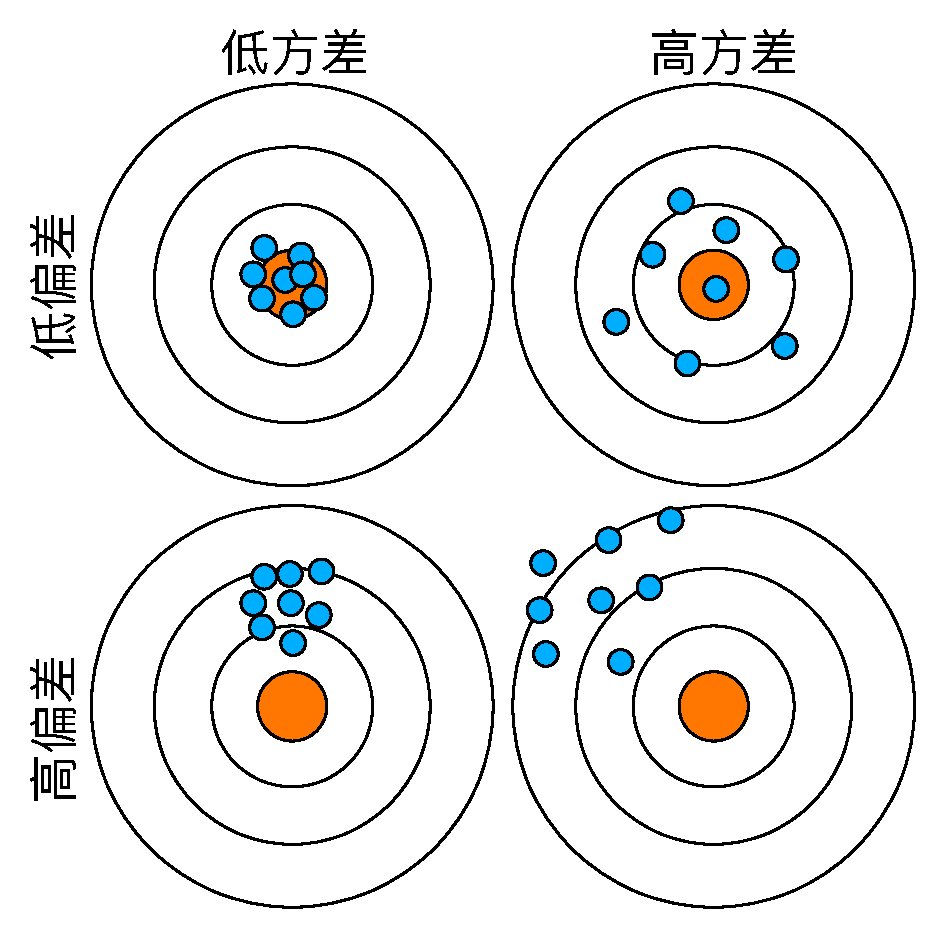
\includegraphics[width=0.45\textwidth]{figures/pt/bias-variance}
	\caption{方差表述的是各随机量和其期望之间的差异,因此低方差随机变量的分布更靠近所有这些随机变量的“中心”(即平均值);偏差则表述的是真实值和期望之间的差异,因此低偏差随机变量的分布更接近于真实值}
	\label{f:pt-bias-variance}
\end{figure}

理论上,我们比较青睐无偏估计,它使整个估计过程中随机量的分布都以真实值为中心,结果永远是正确的,然而这在实践中可能非常困难。首先注意,估计量的偏差$B(I_N)$是和参与估计计算的采样数量是无关的,因此无偏估计要求对于任意给定的数量$N$的估计都是无偏的,从物理意义上讲,它基本上要求估计量和被积函数在形状上是完全相似的;其次,无偏和另一个估计误差的来源,即估计量的方差$V(I_N)$,是一对矛盾,低偏差意味着估计量对被积函数的形状拟合度非常高,使得各个估计值的分布更分散,因此估计的方差更高;此外,高拟合度的估计量也使得整个计算的成本更高。

因此,在图形渲染中,有时候我们寻求更快速的有偏估计,然而在有偏差的情况下,我们能否以及怎样保证最终估计结果的正确性呢,最好的情况是希望估计的偏差能够随着采样数量$N$的增大而逐渐减少甚至消失,这就涉及估计的另一个属性,即一致性(consistency)\myindex{一致性}{consistency}。

对于被估量$I$的一个估计$I_N$是一致的(consistent)\myindex{一致的}{consistent}是指,当采样数量$N$达到无穷大时,估计量$I_N$收敛到$I$的概率为1,即:

\begin{equation}
	P\{\lim_{N\to \infty}I_N(x_1,x_2,\cdots,x_N)\}=1
\end{equation}

虽然无偏估计是更受欢迎的,但是它不应该引入更大方差,否则我们需要花费更大的代价去消除由于方差导致的错误(例如噪点,回想对于蒙特卡洛估计的,我们需要花费4倍的采样数量来减少2倍的方差)。有了一致性属性,如果我们能够证明一个有偏估计是一致性的,则经过足够的采样数量,有偏估计依然会收敛到正确结果。

在基于蒙特卡洛方法的全局光照算法中,我们可以使用这两个属性去衡量各种不同的采样方法,通常对于离线算法,一致性是必须满足的条件。对于有偏性,无偏的算法往往对产品开发流程比较友好,因为离线渲染的时间往往非常长,无偏估计保证无论什么数量的采样都会得到正确的结果,因此我们可以在产品开发阶段使用更少(因此更快)的采样数量来开发产品,而在发布时在使用更多的采样得到更高质量的图像。此外,无偏的估计通常具有更少的参数,整个开发流程也会更加简便;有偏的估计通常具有更快的渲染速度,但是它通常涉及更多的参数控制,以及我们可能很难预期偏差到什么时候减少到了可接受的程度,例如梅特波利斯算法通常很难消除早期阶段的偏差。关于有偏性及一致性更多的一些论述以及理解误区可以参见\cite{a:FiveCommonMisconceptionsaboutBiasinLightTransportSimulation}这篇论文。



 

\section{光线追踪技术及其历史}\label{sec:pt-history}
本节我们首先简要介绍光线追踪技术发展的一些历史,它可以使我们对当前主流离线渲染解决方案的路径追踪技术有更清晰的理解。

回忆一下第1章中关于光与表面交互部分的内容,在我们所处的真实世界中,光遵循一些光学和电磁学中的原理,带着一定能量的光束从光源或其他发光体中发出,它在场景中穿梭,最终击中某个表面;这个表面可能会吸收该光束的一部分能量,导致从该表面反射或散射的光束的能量密度降低,它也可能将全部能量从一个或多个方向反射出去;如果该表面是透明或半透明的,其中一部分光还会以一个不同的方向折射进入该物体内部,在这个过程中部分或全部光能量可能被吸收,最终从物体的另一个表面位置散会回到表面外;此过程不断推进,直到光束被进入传感器装置或者全部被吸收。

这里有必要解释几个概念,一个光束(ray)的度量通常是辐射亮度$L$,通过第1章中的内容知道它表述的是某个方向单位面积的辐射通量(即单位时间的能量),单位为$W/(m^2\cdot sr)$;当光束与表面交互时,表面的材质属性决定了光被怎样吸收和反射,这些交互现象通常划分为两大类,即漫反射和高光反射,漫反射通常对不同的颜色分量(波长)具有不同值,所以光束经过漫反射后的颜色是发生变化的,而对于高光反射,非金属物体的反射率通常和波长无关,所以通常表现为不改变光束的颜色,而仅使其密度减少。更多关于光与表面交互的知识可以参考第1章的内容。

\begin{figure}
\sidecaption
	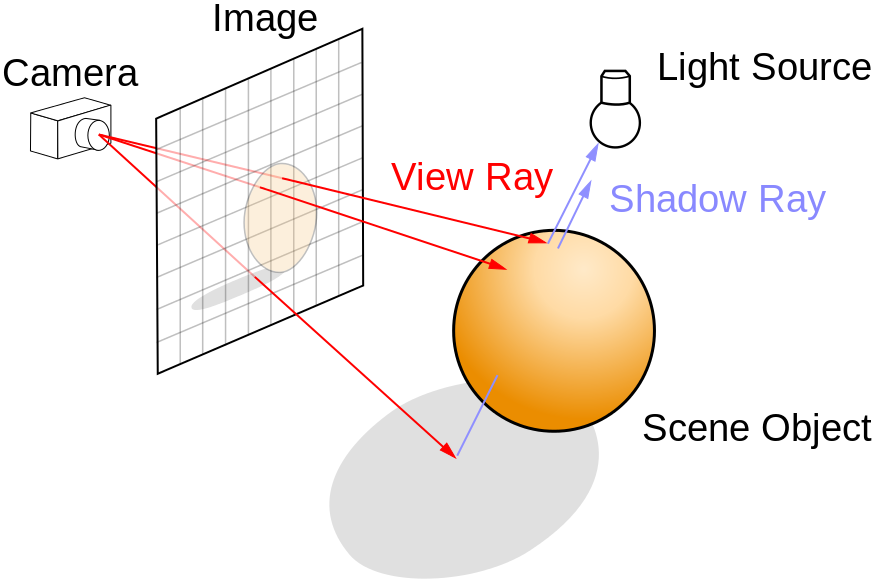
\includegraphics[width=0.45\textwidth]{figures/pt/path-1}
	\caption{光线追踪算法通过构造从摄像机发出并穿过屏幕像素的光线来构造合成图像(图片来自Wikipedia)}
	\label{f:pt-ray-tracing}
\end{figure}

光线追踪(ray tracing)\myindex{光线追踪}{ray tracing}是一种用来根据一定的场景描述生成计算机合成图像的技术,它通过模拟自然界光的传输过程,但是与之相反的是,它通过以摄像机为起点,朝着屏幕每个像素点的方向发射光线,这些光线在场景中与表面进行交互与传播,最终击中一个光源或发光体,如图\ref{f:pt-ray-tracing}所示。

尽管光线在场景中会按照光学规律经过多次反弹才会与光源或发光体相遇,然而早期限于计算机硬件性能以及光照算法的发展,我们并不能模拟完整的光照传输。最早的光线追踪技术称为光线投射(ray casting)\myindex{光线投射}{ray casting} \cite{a:Sometechniquesforshadingmachinerenderingsofsolids},如图\ref{f:pt-ray-tracing}所示,它首先从摄像机发出一条可视光线(view ray)以找到场景中每个像素的可视点,然后从这个可视点向光源发射一条阴影光线(shadow ray)\myindex{阴影光线}{shadow ray}以求出该可视点的颜色,光线投射技术是对渲染方程的以下近似:

\begin{equation}
	L(p,\omega_o)=L_e(p, \omega_o)+\sum_{i=1}^{N_L}L(p,\omega_i) f_r(p,\omega_o,\omega_i)|\cos\theta_i|
\end{equation}

\noindent 在以上公式中,$N_L$代表光源的数量,该式计算的其实就是直接光源。尽管光线投射算法非常简单,但是它建立了以后光线追踪技术的一个基本步骤,那就是从某一个点沿某个方向发出一条光线,然后求出该光线与场景中的哪一个表面相交。\cite{a:ray-tracing}就在光线投射的基础上,让光线沿反射或折射方向继续递归地传播,直到遇到光源为止。在该算法中,当一个光线击中一个表面时,它随机产生3条光线,即反射光,折射光和阴影光线,如图\ref{f:pt-recursive-ray-tracing}所示。

\begin{figure}
\sidecaption
	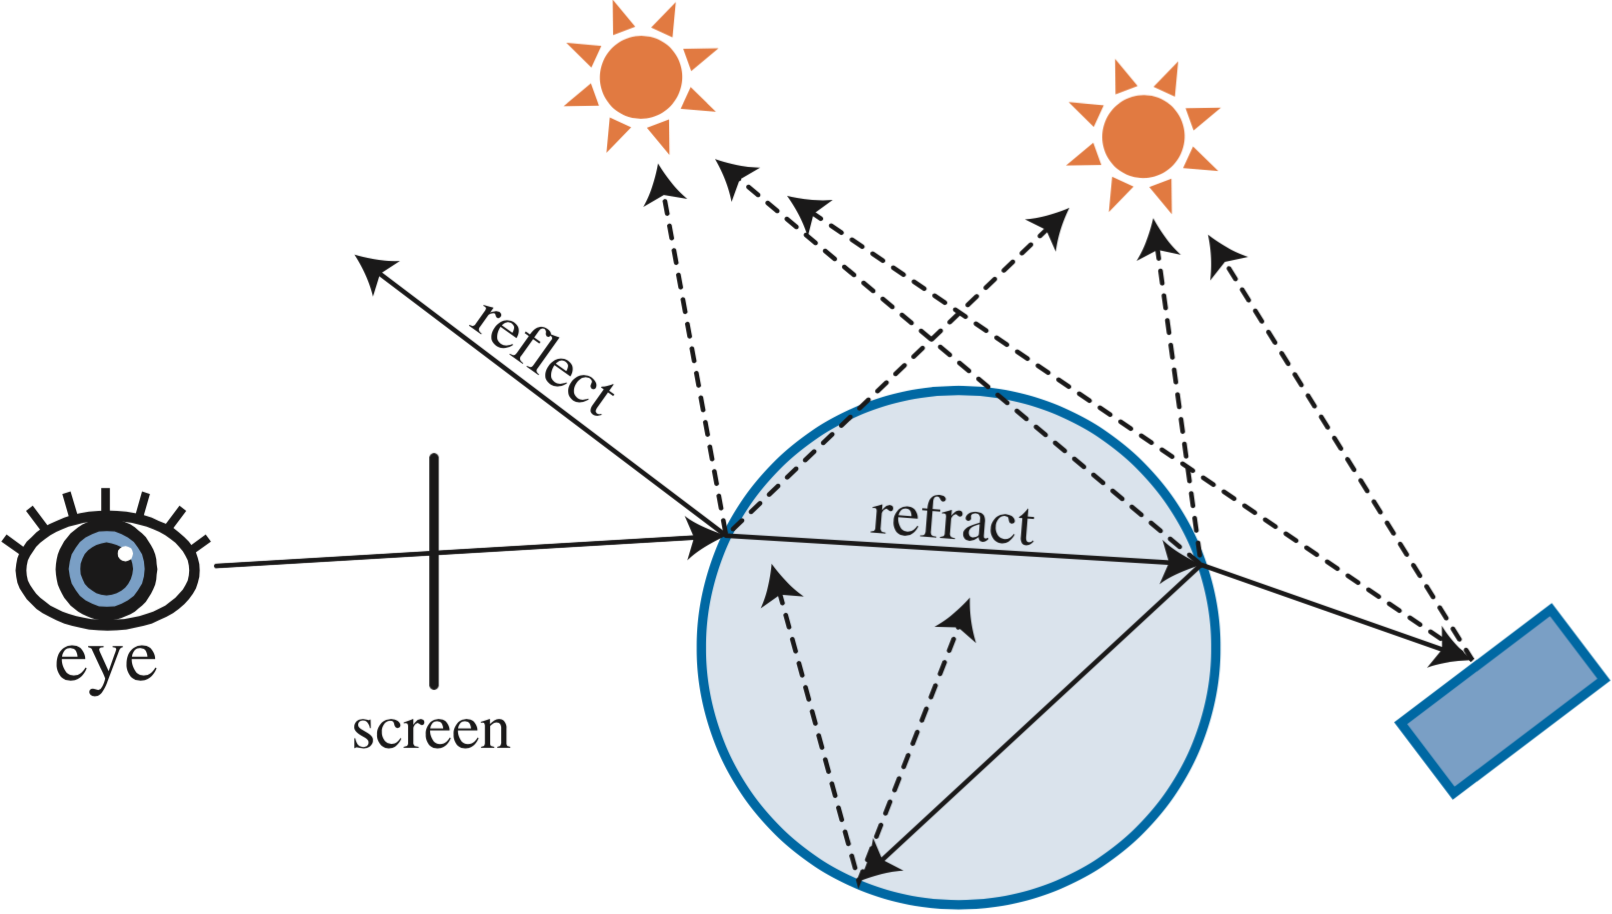
\includegraphics[width=0.6\textwidth]{figures/pt/path-2}
	\caption{一条光线从摄像机出发穿过屏幕区域的像素点进入场景,当它击中每个表面时,立即产生3条新的光线:反射光,折射光和阴影光线,这个过程递归继续进行,它会产生越来越多的光线。(图片来自\cite{b:rtr})}
	\label{f:pt-recursive-ray-tracing}
\end{figure}

这个确定性的(以区别于后面基于蒙特卡洛方法的随机形式)光线追踪的形式称为Whitted风格的光线追踪(Whitted-style ray tracing)\myindex{Whitted风格的光线追踪}{Whitted-style ray tracin},也称为递归光线追踪(recursive ray tracing)\myindex{递归光线追踪}{recursive ray tracing},它实现以下形式的光照传输:

\begin{equation}
\begin{aligned}
	L(p,\omega_o)=&L_e(p, \omega_o)+\sum_{i=1}^{N_L}L(p,\omega_i) f_r(p,\omega_o,\omega_i)|\cos\theta_i|\\
	&+L_r(p,\omega_r)f_r(p,\omega_o,\omega_r)|\cos\theta_r|
\end{aligned}
\end{equation}

Whitted风格的光线追踪在光线投射算法的基础上加入了间接光照,但是这些间接光照仅限于完全的镜面反射和折射,因为它在反射和折射方向上只拾取一个方向,即它假设物体表面是绝对光滑的,因此该算法中的反射系数BRDF是一个狄拉克函数\footnote{狄拉克函数又称为脉冲函数,它表示在一个给定定义域上只有一个点是非零的,其他点的值都为0。}(dirac function)\myindex{狄拉克函数}{dirac function},即在一个给定的空间方向定义域中,该BRDF只在一个方向上是非零的。

上述限制被\cite{a:DistributedRayTracing}的分布式光线追踪算法(distribution ray tracing)\myindex{分布式光线追踪算法}{distribution ray tracing}克服, 该算法基于空间中所有方向的一个积分来近似光泽反射(glossy reflection)\myindex{光泽反射}{glossy reflection},以及使用基于光源面积范围内的方向的积分来计算软阴影效果。在该算法中,它们使用蒙特卡洛方法来近似计算这些积分值,所以该算法又称为随机光线追踪(stochastic ray tracing)\myindex{随机光线追踪}{stochastic ray tracing},该算法实现以下形式的光照传输:

\begin{equation}
\begin{aligned}
	L(p,\omega_o)=&L_e(p, \omega_o)+\sum_{i=1}^{N_L}{\rm \int}_{\Omega_i}L(p,\omega_i) f_r(p,\omega_o,\omega_i)|\cos\theta_i|{\rm d}\omega_i\\
	&+{\rm \int}_{\Omega_r}L_r(p,\omega_r)f_r(p,\omega_o,\omega_r)|\cos\theta_r|{\rm d}\omega_r
\end{aligned}
\label{eq:pt-distribution}
\end{equation}

分布式光线追踪算法第一次引入蒙特卡洛方法用于计算更完整的光照传输,由第1章的内容可知,物体的表面并不是绝对光滑的,在小于一个像素的微观层面,存在很多大于波长的微观面元,因此一束光经过一个像素大小的表面反射或折射后,会被分布到多个方向上,因此反过来看,就是每个出射方向的辐射亮度是由来自多个方向的入射光构成的,这就涉及针对空间方向的积分计算,蒙特卡洛方法的引入简化了这个积分计算。

如图\ref{f:pt-distribution-ray-tracing}所示,在分布式光线追踪算法中,当一束可视光线与某个表面点时,由式\ref{eq:pt-distribution}可知,它的结果是对来自空间多个方向的辐射亮度的积分,即是在蒙特卡洛方法中需要从空间中抽取多个方向。因此,一条从摄像机发出的光线被拆分成多条反射光,折射光以及阴影光束,即分布式光线追踪导致了一条树形的光束树,随着光线的递进,光线数量会发射得越来越多。

\begin{figure}
\sidecaption
	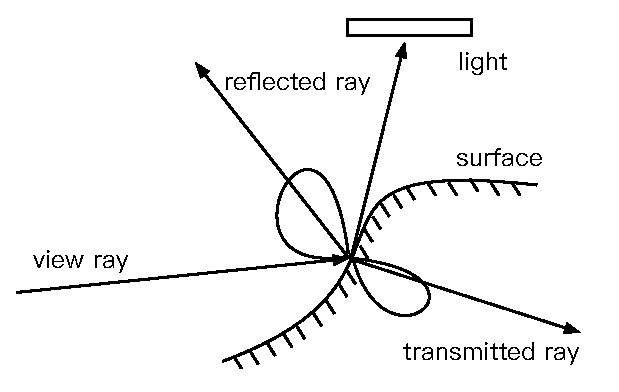
\includegraphics[width=0.5\textwidth]{figures/pt/distribution}
	\caption{在分布式光线追踪算法中,一条可视光线的辐射亮度是来自多条入射光的蒙特卡洛估计,对于反射和折射光是在该光束各自对应的法线方向的半空间内对方向的采样,而阴影光束则是在光源范围内的方向采样}
	\label{f:pt-distribution-ray-tracing}
\end{figure}

这种光线发散的方式是分布式光线追踪最大的缺点,它使得几乎不可能计算间接漫反射(indirect diffuse)光照,因为每一单束光都需要对整个半空间进行积分计算。

分布式光线追踪的这种特点是和递归的原始光照公式形式有关的,这是一个非常隐式的公式:要想计算某个方向的入射光,需要首先计算能够对该方向形成贡献的所有方向的入射光,整个场景中的光照分布被隐藏在一层一层递归的层次中。直到\cite{a:TheRenderingEquation}将光照公式转换成了一个基于路径积分形式的,显式积分方程,光照传输的计算才能够被有效地使用蒙特卡洛方法进行计算,在路径积分形式的光照公式中,整个场景的光照分布就是一条条路径的积分,不再有隐式的递归,只要我们找到足够数量的路径,就能够使用蒙特卡洛方法有效地计算光照分布。基于这种路径积分形式的全局光照技术通常称为路径追踪(path tracing)\myindex{路径追踪}{path tracing},它是当前主流渲染器的基础,它能够有效地处理大部分光学现象,包括间接漫反射,散射,间接光,焦散效果等。下一节,我们就将首先推导光照公式的路径积分形式,它是我们接下来几章的重要基础。







\section{光照公式的路径积分形式}\label{sec:pt-surface-form}
全局光照计算本质上是关于计算光照传输的问题,光源发射出一些携带者能量的光束在3D场景中传播,当这些光束遇到物体表面时以反射或者折射的方式和表面进行交互,然后这些被反射的光束继续在场景中传播,直到系统处于平衡状态,此时就呈现出我们看到的图像。在这个计算过程中,我们要保证的就是光照的传输保持能量守恒(energy equilibrium)\myindex{能量守恒}{energy equilibrium}。

因为我们人眼或传感器接收的是辐射亮度这个物理量,所以为了保证能量守恒,很自然的形式就是对于每个点$p$,它朝某个方向$\omega_o$发射出的辐射亮度$L_o$,应该等于该点接收来自所有入射方向$\omega_i$的辐射亮度$L_i$的和,在出射方向的$\omega_o$的一个分量,这个分量的大小由BRDF控制(注意BRDF是与波长有关的),所以如第1章所看到的,传统基于半空间方向积分形式的光照公式如下:

\begin{equation}\label{e:hemisphere-formulation}
	L(p,\omega_o)=L_e(p,\omega_o)+{\rm \int}_{\Omega}f(p,\omega_o,\omega_i)L(t(p,\omega_i),-\omega_i)|\cos\theta_i|{\rm d}\omega_i
\end{equation}

\noindent 与第1章中的形式略微不同的时,第1章的入射光辐射亮度只是用一个方向表示$L_i(p\leftarrow\omega_i)$,那里仅是为了使我们将注意力放在光照公式形式上而不是怎样去解这个光照公式,而当开始去解光照公式时,我们需要知道这个方向是来自场景中哪个表面上的点,所以需要做的是从点$p$沿$\omega_i$反方向投射一条光线,然后看该光线与场景中哪个点相交,这正是上一节讨论的各种光线追踪算法中的基本步骤。所以在这里,我们将这个光线投射函数(ray-casting function)\myindex{光线投射函数}{ray-casting function}$t(p,\omega)$集成在光照公式中,它表示的是沿$p$点沿$\omega_i$反方向发射一条光线得到的第一个与该光线相交的点。

式\ref{e:hemisphere-formulation}表示的光照公式是一个隐式方程\footnote{隐式方程是指光照公式并不是一个直接的积分形式,这种隐性增加了算法的复杂性,例如我们不能简单地使用一个单一的蒙特卡洛方法进行积分近似,而是需要无数个蒙特卡洛来完成这个迭代公式的计算,大大增加了算法复杂度。},即要想求得某一点$p$沿某方向$\omega_o$的辐射亮度,必须首先求出从所有方向达到$p$点的辐射亮度,以此类推,这种递归的形式就形成了分布式光线追踪这样的算法。

\begin{figure}
	\sidecaption
	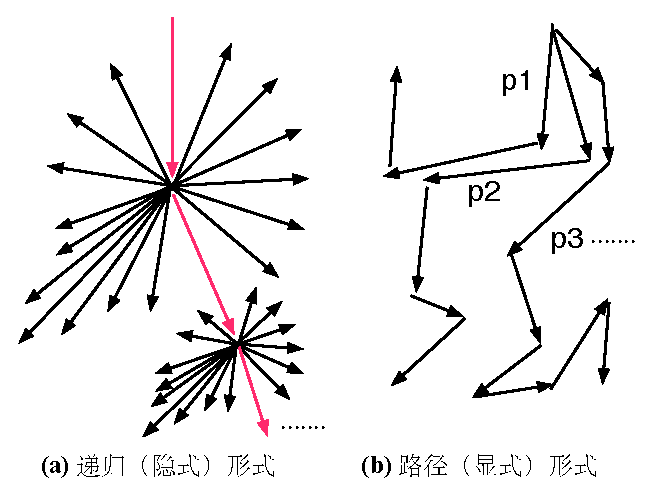
\includegraphics[width=0.6\textwidth]{figures/pt/path}
	\caption{由分布式光线追踪中的光线树可知,光照计算其实本质上是无穷多个光线路径的积分,因此我们希望能够推导出这种显式的路径积分形式,它不仅可以保证计算是无偏的,并且简化了积分形式,使得我们可以使用对路径进行采样的方式来直接计算光照分布}
	\label{f:pt-path}
\end{figure}

分布式光线追踪形成了一颗光线树,如图\ref{f:pt-path}(a)所示,虽然理论上经过足够的时间以产生足够的光线数量以及足够深度(多次反弹的光线)的光线数量后,光照传输的结果会趋近于真实的平衡分布,但是由于漫反射表面形成的全空间积分,这个逼近过程会非常慢,并且早期的图像是偏差非常大的,这非常不利于产品开发。

直观上理解,分布式光线追踪算法的结果其实是无穷条光线路径的积分,这些路径对应于光线树上的所有分支构成的光线,因此如果我们将这些路径抽取出来(如图\ref{f:pt-path}(a)中的红色线条),就能够形成一个显式的路径积分形式,所以它们两种形式在数学上是等效的。但是重要的是,路径形式的积分使我们一开始就能够看到整个分布,如图\ref{f:pt-path}(b)所示,我们可以在一开始只有少量光线的情况下就能够得到足够深度的光线,使得整个积分是无偏的,随着路径采样数量的增加,两种形式会趋向相同的结果\footnote{直观上看,路径积分形式将一些重要的路径提前采样出来,例如那些高光路径,它们会有更大的概率被选中,然后才是在逼近过程中逐步增加贡献小的漫反射路径,因此它一开始的结果就是正确的,即符合平衡分布的。}。

那这种路径积分形式应该怎样转换呢?基于半空间方向积分形式的光照公式中,每一步都是一个方向,显然我们不可能把这些方向抽取出来组成一条路径,一条路径是由多个顶点构成的,因此我们需要把光照公式从基于方向的积分形式转变变基于表面的路径形式,然后我们可以对这些表面进行采样得到路径的顶点。

\begin{figure}
	\sidecaption
	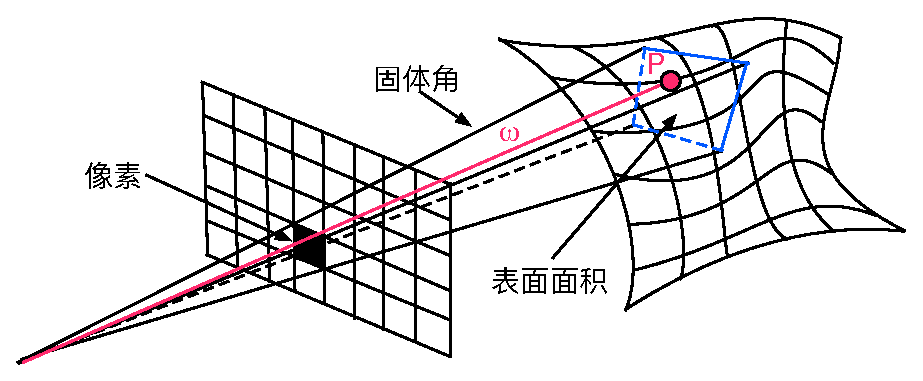
\includegraphics[width=0.65\textwidth]{figures/pt/solid-angle-to-surface}
	\caption{光照公式的半空间方向积分形式和面积积分在数学上是等效的,因为一个立体角表示的就是空间中方向的集合,它可以用一个截面的面积来表示,所以对空间方向的采样等效于对这个截面中点的采样,这就是路径积分形式的基础}
	\label{f:pt-solid-angle-to-surface}
\end{figure}

回忆立体角(solid angle)\myindex{立体角}{solid angle}的定义,它表示的是空间中方向的一个集合,就好比2D空间中方向的集合构成一个角度一样。立体角的度量可以使用这个方向集合对应的空间单位球面上的截面面积来表示,就像2D空间中角度用单位圆上的弧长表示一样,因此我们可以将一个方向集合转变成一个面积的形式,这样就可以将半空间方向积分形式的光照公式转变成面积积分形式的光照公式,如图\ref{f:pt-solid-angle-to-surface}所示。这样,方向积分形式的光照公式中对一个方向空间进行采样,就等效于面积积分形式中对面积进行采样,即一个点。而有了这个点的表示,我们就可以将光线树中的路径提取并表述出来。

所以,光照公式的方向积分和面积积分形式在数学上是完全等效的,这也是光照公式的两种基本形式。面积积分形式的光照公式是路径追踪技术的基础,实际上,在后面的章节中我们还可以看到,很多不同的全局光照技术就是基于不同形式的光照公式来进行光照计算的,读者可以参考\cite{b:AdvancedGlobalIllumination}中更多关于光照公式不同形式的推导和介绍。






\subsection{光照公式的面积积分形式}
根据前面的分析,面积形式的光照公式的转换需要做两件事情,首先是将被积函数中的方向相关的变量转换为点相关的变量,其次是将自变量$\omega$的微分${\rm d}\omega$转换成点$p$的微分,即面积$dA$。

\begin{figure}
	\sidecaption
	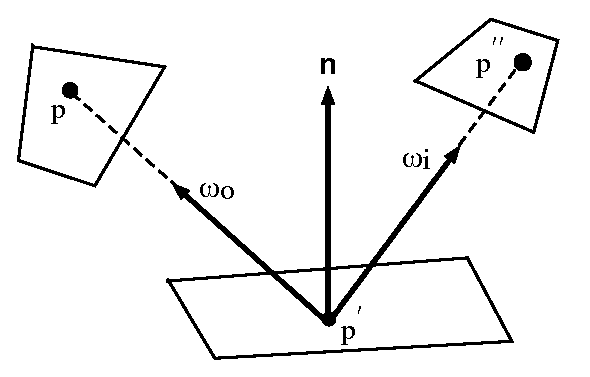
\includegraphics[width=0.52\textwidth]{figures/pt/three-point-form}
	\caption{三点形式的光照传输方程是将基于方向的积分形式转换为基于面积的积分形式的关键,它将被积函数中的方向变量转换为路径的顶点,这样顶点连接就可以构成路径}
	\label{f:pt-three-point-form}
\end{figure}

式\ref{e:hemisphere-formulation}中的被积函数是用方向表示的,这样我们才能表示来自某个方向的辐射亮度,在计算时,这个方向被用作光线投射函数的参数以计算该光线是来自场景中的那个点。所以,如果能够提前知道这个光线的交点,则可以直接用点表示辐射亮度,因为它们都可以唯一表述一个辐射亮度,如图\ref{f:pt-three-point-form}所示。这样从场景中一点$p^{'}$到点$p$的辐射亮度可以表示为:

\begin{equation*}
	L(p^{'}\to p)=L(p^{'},\omega)
\end{equation*}

同理,如果点$p^{'}$和$p$是相互可见的,并且$\omega_o=\widehat{p-p^{'}}$以及$\omega_i=\widehat{p^{'}-p^{''}}$,我们也可以用点(位置)的形式表示点$p^{'}$处的BRDF函数为(如图\ref{f:pt-three-point-form}所示):

\begin{equation*}
	f(p^{''}\to p^{'}\to p)=f(p^{'},\omega_o,\omega_i)
\end{equation*}

\begin{myshaded}
	光线投射函数\myindex{光线投射函数}{ray-casting function}去哪里了?在基于空间方向的积分形式中,光线投射函数被集成在光照公式中,所以我们看到在分布式光线追踪算法中,它的每一个方向采样都需要执行这个光线投射函数以找出光线的交点。
	
	\indent 然而,在路径形式的积分中,光线投射函数直接被路径顶点取代了,这是否意味中路径追踪算法中不再执行光线投射计算?当然不是,通过前面的分析,方向积分形式和路径积分形式的光照公式在数学上是完全等效的,所以它们都必须通过光线投射来找到合适的光线路径。但是这里有个重要区别,路径形式的光照公式将光线投射函数从光照积分中抽取出来,我们首先使用光线投射函数来寻找路径的各个顶点,然后这些顶点被连接起来构成一条路径,这个路径作为整个光照积分公式的“采样点”。也正是将光线投射函数的计算从光照积分中分离出来,才能获得一个直接,显式的基于路径的光照积分公式。
\end{myshaded}

接下来,我们需要将方向微分${\rm d}\omega$转换为面积微分${\rm d}A$。根据立体角的定义,如果一个球面上的任意一块区域的面积$A$等于该球半径$r$的平方,则从该球球心位置观察,该区域面积对应的立体角大小就是$1sr$,因此球面上面积$A$对应的立体角为$ \cfrac{A}{r^{2}}$。由于场景中任意面积$A$可能并不与半径方向垂直,所以计算时需要首先将面积$A$投影到以$d$为半径的球面上,在使用该投影面积求得对应的立体角,综上所述,结合图\ref{f:pt-solid-to-area}所示,任意面积$A$对应的立体角为:

\begin{equation}
	\omega= \cfrac{A\cos{\theta^{'}}}{d^2}
\end{equation}

\noindent 将此变量变换形式代入带方向积分形式的光照公式中,就可以得到面积积分形式的光照公式。为了简化最终光照公式的形式,我们将上述立体角的转换式,原始光照公式中的$|\cos\theta|$项,以及一个可见性函数$V$(其中当两个点相互可见时$V=1$,否则$V=0$)组合成一个单一的几何项$G(p\leftrightarrow p^{'})$:

\begin{equation}
	G(p\leftrightarrow p^{'})=V(p\leftrightarrow p^{'}) \cfrac{|\cos\theta||\cos\theta^{'}|}{||p-p^{'}||^2}
\end{equation} 

\noindent 代入上述几何项到原始光照传输方程中,得到最终的面积积分形式的光照公式:

\begin{equation}\label{e:integral-over-area}
	L(p^{'}\to p)=L_e(p^{'}\to p)+{\rm \int}_A f(p^{''}\to p^{'}\to p)L(p^{''}\to p^{'})G(p\leftrightarrow p^{'}){\rm d}A(p^{''})
\end{equation}

\noindent 这里$A$表示场景中所有的表面。

\begin{figure}
	\sidecaption
	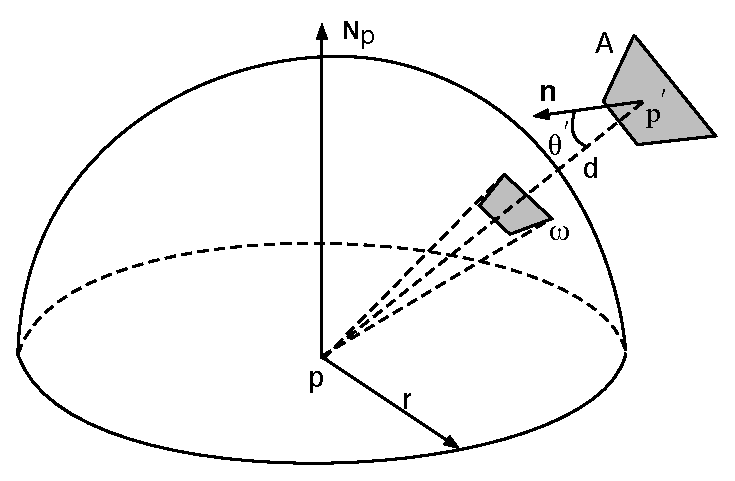
\includegraphics[width=0.55\textwidth]{figures/pt/solid-to-area}
	\caption{从点$p$观察,与点$p$距离为$d$的任意面积$A$的立体角,等于该面积在以$p$为球心,$d$为半径的球面上的投影面积所对应的立体角的大小}
	\label{f:pt-solid-to-area}
\end{figure}

虽然式\ref{e:hemisphere-formulation}和\ref{e:integral-over-area}在数学上是等效的,但是它们分别代表了光线追踪和路径追踪两种不同的全局光照算法的思路。在光线追踪算法中,我们需要递归地对每一条光线的空间分布使用蒙特卡洛方法进行采样,而在路径追踪算法中只需要以适当的方式对路径采样,然后使用蒙特卡洛方法直接计算光照分布。这些对路径的不同的采样方式构成了路径追踪算法的重要内容,我们将在后面的内容中详细讨论,在此之前,我们需要首先了解什么是一条路径。






\subsection{路径积分形式}
有了上一节光照公式的面积形式,每个迭代中的项直接显式地使用场景中某个表面点进行表述,而不是隐藏在光线投射函数中,所以我们可以通过不断地将式\ref{e:integral-over-area}中右边的项代入被积函数中的入射辐射亮度$L(p^{''}\to p^{'})$,得到如下形式的光照公式:

\begin{equation}
	\begin{aligned}
		L(p_1\to p_0)=&L_e(p_1\to p_0)\\
		&+{\rm \int}_AL_e(p_2\to p_1)f(p_2\to p_1\to p_0)G(p_2\leftrightarrow p_1){\rm d}A(p_2)\\
		&+{\rm \int}_A{\rm \int}_A L_e(p_3\to p_2)f(p_3\to p_2\to p_1)G(p_3\leftrightarrow p_2)\\
		&\qquad\qquad \times f(p_2\to p_1\to p_0)G(p_2\leftrightarrow p_1){\rm d}A(p_3){\rm d}A(p_2)+...
	\end{aligned}
	\label{e:pt-path-form}
\end{equation}

\noindent 这里$p_0$表示摄像机位置,$p_1$表示从摄像机出发沿$p_1-p_0$方向发射的光线与场景物体的第一个交点。式\ref{e:pt-path-form}中右边的每一项表示一个长度不断递增的路径,例如第3项可以由图\ref{f:pt-a-path}所示的路径表示,它表示长度为3的所有路径,也即是所有经过2次反弹的间接光照。

\begin{figure}
\sidecaption
	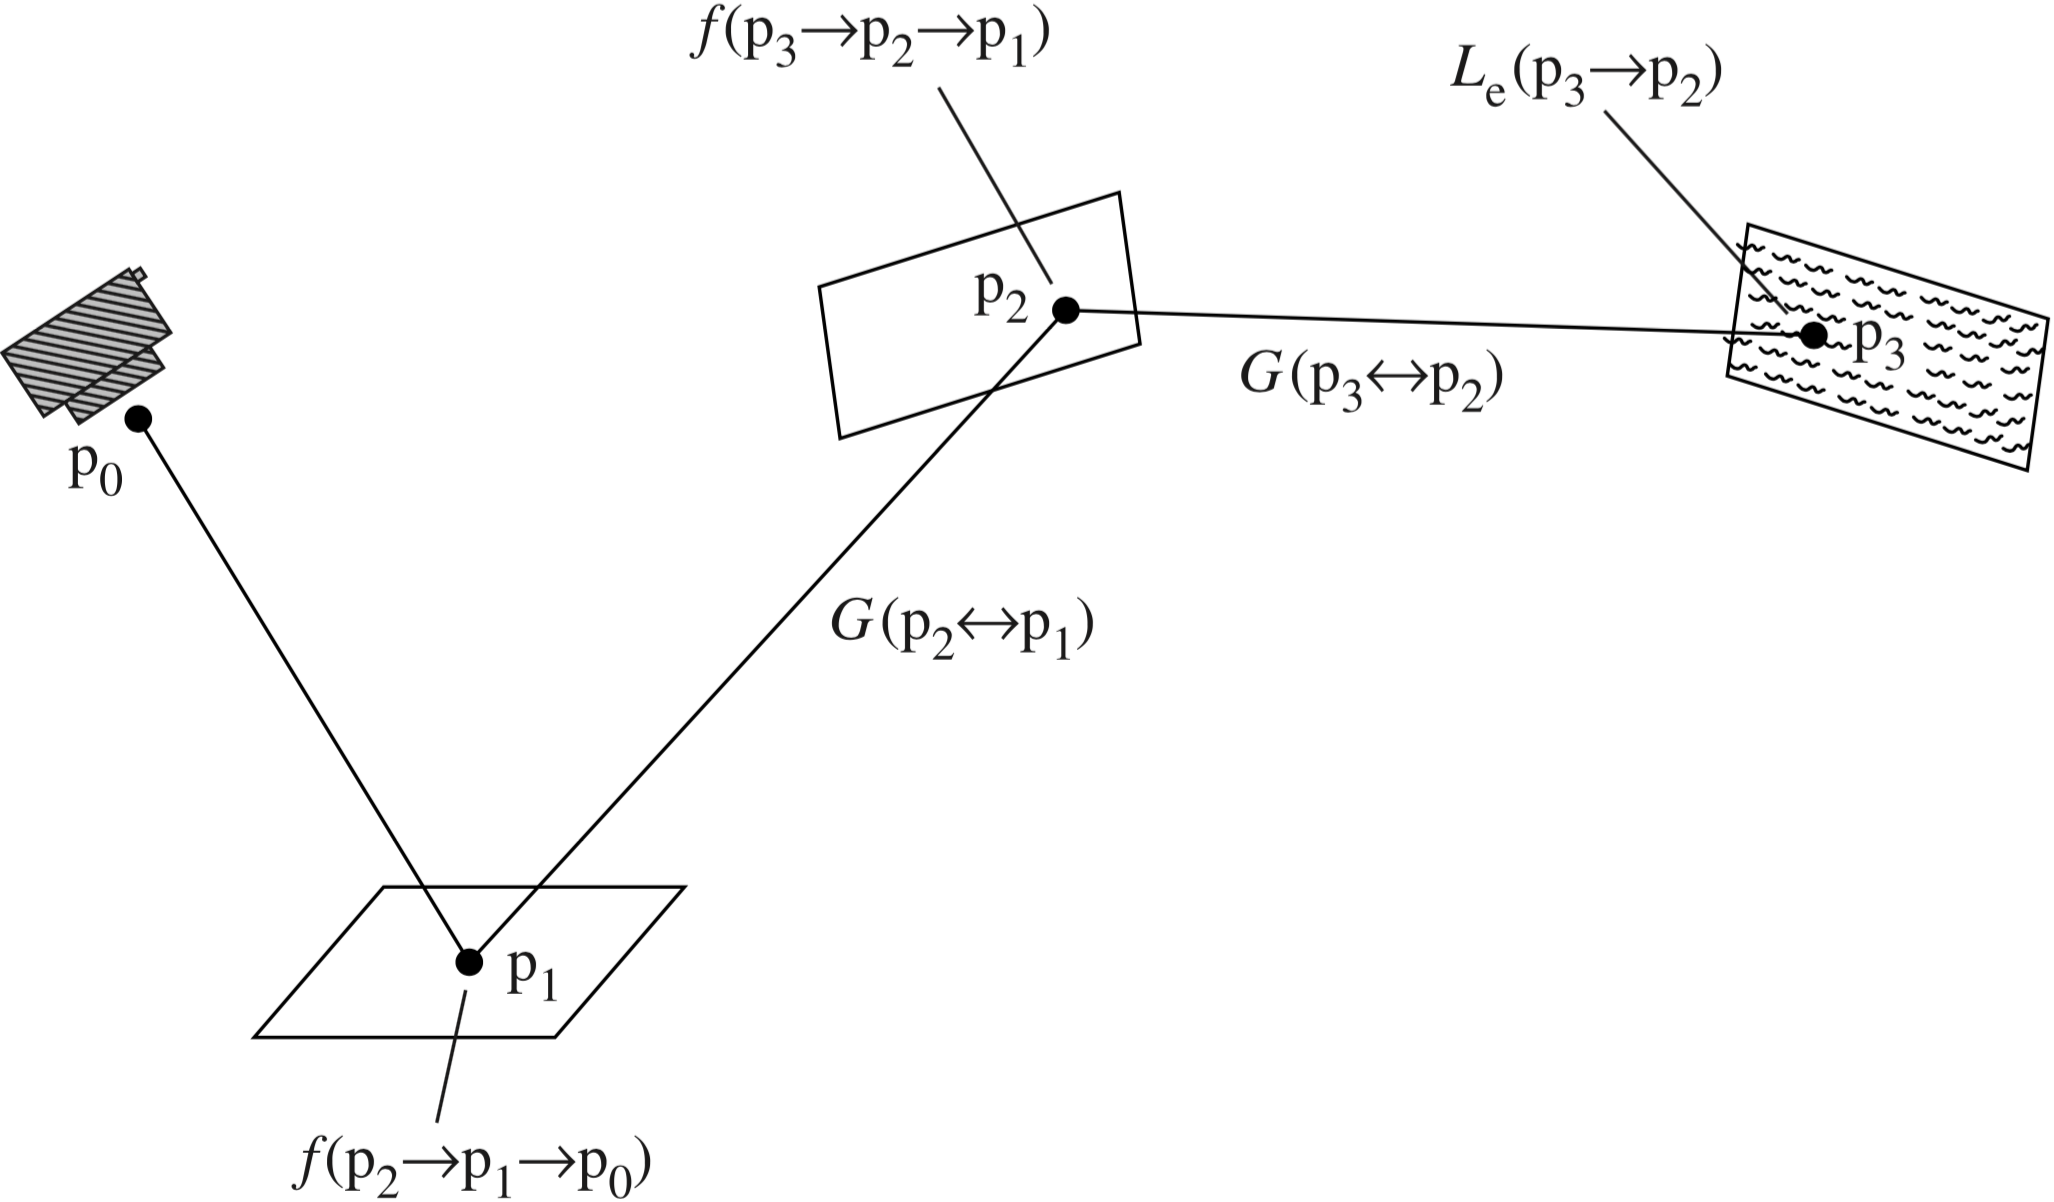
\includegraphics[width=0.65\textwidth]{figures/pt/path-5}
	\caption{所有由点$p_2$和$p_3$组成的路径,就构成了$p_1$向$p_0$方向的辐射亮度中两次反弹的间接光照,这里列出了被积函数乘积的每个分量:光源发出的辐射亮度$L_e$,路径顶点之间的几何分量$G$,以及每个表面的BRDF函数}
	\label{f:pt-a-path}
\end{figure}

既然式\ref{e:pt-path-form}中的每一项可以表示为一条由多个顶点组成的路径,所以我们可以将上述无限项的和的形式简写为下述紧凑的形式:

\begin{equation}\label{e:path-form}
	L(p_1\to p_0)=\sum_{n=1}^{\infty}P(\bar{p}_n)
\end{equation}

\noindent 这里$P(\bar{p}_n)$表述的是一条具有$n+1$个顶点的路径$\bar{p}_n$对辐射亮度的贡献,其中一条路径的形式为:$\bar{p}_n=p_0,p_1,...,p_n$,这里$p_0$表示的是摄像机位置,而$p_n$是光源上的一个采样点。 $P(\bar{p}_n)$具有如下形式:

\begin{equation}
	\begin{aligned}
		P(\bar{p}_n)=&\underbrace{{\rm \int}_A{\rm \int}_A \cdots{\rm \int}_A}_{n-1}L_e(p_n\to p_{n-1})\\
		&\quad\times\Bigg(\prod_{i=1}^{n-1}f(p_{i+1}\to p_i\to p_{i-1})G(p_{i+1}\leftrightarrow p_i)\Bigg) {\rm d}A(p_2)\cdots {\rm d}A(p_n)
	\end{aligned}
\end{equation}

\noindent 在上式中,沿路径上每个点处所有BRDF函数的乘积表示的是路径的吞吐量(throughput)\myindex{吞吐量}{throughput},它表示该路径中光源发出的辐射亮度沿该路径传递到摄像机的分量,我们可以定位该吞吐量为以下标记:

\begin{equation*}
	T(\bar{p}_n)=\prod_{i=1}^{n-1}f(p_{i+1}\to p_i\to p_{i-1})G(p_{i+1}\leftrightarrow p_i)
\end{equation*}

\noindent 那么一条路径$\bar{p}_n$的辐射亮度贡献就可以简写为:

\begin{equation*}
	P(\bar{p}_n)=\underbrace{{\rm \int}_A{\rm \int}_A \cdots{\rm \int}_A}_{n-1}L_e(p_n\to p_{n-1})T(\bar{p}_n) {\rm d}A(p_2)\cdots {\rm d}A(p_n)
\end{equation*} 

\noindent 这是一个维度为$n-1$的高维积分,因此式\ref{e:path-form}可以解释为由多个特定路径长度$n$对应的高维积分的和。所以对于每一个路径长度$n$对应的$P(\bar{p}_n)$,我们可以使用蒙特卡洛方法来计算该高维积分,这非常简单,每一个采样样本就是一个$n-1$维向量,我们称这个向量所在的空间为路径空间(path space)\myindex{路径空间}{path space},在这里它可以是随机抽取场景中的$n-1$个点组成一个长度为$n$的路径$\bar{p}_n$,该路径样本对应的概率密度由其$T(\bar{p}_n)$决定。

路径追踪技术中的路径有各种各样的采样方式,不同的采样方式其蒙特卡洛估计的收敛速度差异可能非常大,路径追踪技术大部分的研究都涉及更有效地对路径进行采样,我们可以在本章以及接下来的章节看到很多不同的路径采样技术。





\subsection{一个像素的颜色如何计算}\label{sec:pt-pixel-filter}
我们可能还是会对上述的路径形式的蒙特卡洛方法有些疑惑,蒙特卡洛方法是用于计算一个积分值的,例如在分布式光线追踪算法中,每一个出射辐射亮度的值是有由半空间上所有方向的入射辐射亮度的积分决定的,因此这是一个很自然的蒙特卡洛方法的应用,但是这里应该怎样解释呢?

分析式\ref{e:pt-path-form}的形式,此时我们假设所有路径都是固定长度为$n$的路径,那么此时有: $L(p_1\to p_0)=P(\bar{p}_n)$,所以这个高维积分的值即是摄像机$p_0$处看到的颜色,注意这个积分值的定义域是整个场景,因此它并不只是一个像素对应方向上的路径,而是所有穿过屏幕的路径构成的这个积分值,所以我们能够使用蒙特卡洛方法。

那么怎样计算单个像素的值呢?虽然这里的整个蒙特卡洛估计是针对全屏幕的,但是这些参与估计的路径样本则是穿过屏幕区域的每一个像素点的,因此每一个路径样本的值就是代表了每个像素位置的值。由于蒙特卡洛方法的样本数量(即路径数量)会远远大于屏幕像素的数量,即是这些路径的结果构成了一个屏幕区域的图像的颜色分布函数,我们要向获得(更低分辨率)单个离散位置的颜色值,就涉及对这个图像分布函数的采样,同纹理的采样类似,这里我们需要使用一个过滤器。通常使用一个简单的盒子过滤器(box filter)\myindex{盒子过滤器}{box filter}即可,它将周围处于这个盒子范围内的路径取平均值来作为该像素的最终颜色值,如图\ref{f:pt-ray-set-up}所示。

\begin{figure}
	\sidecaption
	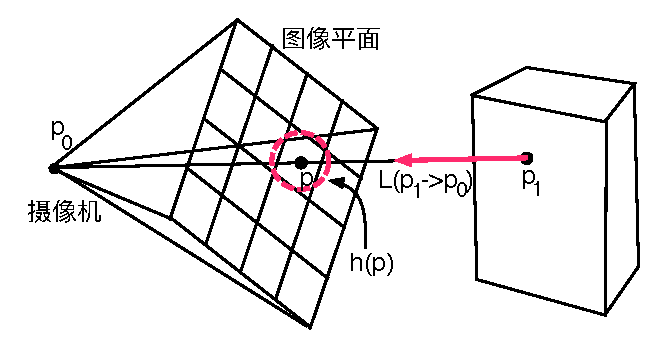
\includegraphics[width=0.55\textwidth]{figures/pt/ray-set-up}
	\caption{路径追踪算法的蒙特卡洛方法计算的结果是整个图像区域的颜色分布,因此我们要得出每个离散像素位置的颜色值,就需要使用一个过滤器,这和其他对函数进行采样的思路是一样的}
	\label{f:pt-ray-set-up}
\end{figure}

根据以上分析,在路径追踪技术中,一个屏幕上像素$p$的颜色最终可以由以下式计算:

\begin{equation}
	L_p={\rm \int}_{imageplane}L(p_1\to p_0)h(p){\rm d}p
\end{equation}

这里$h(p)$是一个过滤器,它会以适当的权重计算每个处于该过滤器范围内的路径辐射亮度贡献值,函数$h(p)$和$L(p_1\to p_0)$之间是一个基于点的卷积计算。计算每个像素的颜色值伪代码如下:

\begin{lstlisting}[language=C++,mathescape]
void ComputeImage(Point eye) {
	for each pixel {
		//注意实际颜色是三个分量
		Color radiance = 0;
		//过滤器的总权重值,用于归一化每一项权重         
		float H = integral(h(p));   
		for each viewingRay {
			//抽取一个过滤器范围内的随机位置
			Point p = RandomPositionWithinRangeOfH(); 
			Ray viewRay = GetDirection(eye, p);
			//计算每一条光线过滤后的值
			radiance += RayRadiance(viewRay)*h(p); 
		}
			
		radiance = radiance / (#viewingRays*H);
	}
}
	
Color RayRadiance(Ray ray) {
	Point x = FindNesarestIntersection(ray);
	return ComputeRadiance(x, ray);
}
\end{lstlisting}


在上述伪代码中,ComputeRadiance正是路径追踪技术中对每一条路径辐射亮度的计算,这涉及怎样对路径进行采样等一些技术,我们将在下一节讨论这些问题。





\section{基本路径追踪技术}\label{sec:pt-basic}
上一节我们讨论了路径追踪技术的基础,即光照公式的路径积分形式,并解释了蒙特卡洛方法怎样用于该积分计算中,以及怎样使用路径追踪技术计算屏幕上每个像素颜色值扥框架,本节我们将讨论路径追踪计算怎样计算一条路径的光照传输。

给定上述路径积分形式,路径追踪算法最基本的两个问题是:怎样以不引人偏差的方式结束无限的路径长度,以及怎样对路径进行采样,其中后者更是几乎是整个路径追踪算法的核心,我们将在本章及后面几章看到非常多不同形式的采样技术,但本节我们节讨论最基本的采样方法。此外,路径追踪技术还涉及如怎样加速光线投射函数的计算,怎样处理纹理的过滤等问题,这些内容将留在后面的高级路径追踪技术中讨论。






\subsection{俄罗斯轮盘}\label{sec:russian-roulette}
对于路径追踪算法中一条给定的从摄像机位置$p_0$出发与场景的第一个交点$p_1$的路径,要计算该路径的光照贡献,我们需要首先解决两个问题:

\begin{enumerate}
	\item 怎样以有限的计算资源来无偏估计具有无限长度形式的路径的贡献值$P(\bar{p}_i)$?
	\item 一旦我们找到一个有限长度的路径形式,对于一个具有有限长度$i$的特定$P(\bar{p}_i)$项,我们应该怎样对场景进行采样以抽取出合适的路径$\bar{p}$来对光照分布进行估计?
\end{enumerate}

本节我们将讨论第一个问题,下一节会介绍路径追踪算法最基本的路径采样方式,而更多更高级的采样方式则会分布在本章及后面的章节中。

对于第一个问题,很显然路径追踪算法需要一个停止条件以抽取一个有限长度的路径,我们可以基于这样的一个观察来解决该问题,即对于物理正确的(例如满足能量守恒条件)光照传输,长度越长的路径其反射的光照(即吞吐量)越小,这是因为为了保证能量守恒,每个点的BRDF函数值总是小于1的,所以我们希望使用某种算法将贡献足够小(即路径足够长)的路径剔除掉。

一个最简单的选择是使用一个固定长度的路径,但是这种方法会引入偏差,因为有些很重要的光照传输可能被忽略了,例如当场景中大部分是高光表面时,一些重要的路径往往会拥有更长的长度。另一个方法是根据路径的贡献适应性地停止路径追踪,每条路径的光照传输都有一个权重系数,这个权重就是由路径上各个顶点出BRDF函数值的乘积,因此随着路径长度的增加,该路径上光源的光照贡献会越来越小,当这个权重小于一定的临界值时,我们就可以截断它,该条路径的追踪到此停止。其中一种流行的方法是俄罗斯轮盘(russian roulette)\myindex{俄罗斯轮盘}{russian roulette}。

为了应用俄罗斯轮盘,我们首先需要选择一个终止概率$q$,在这个终止概率下,被积函数有$q$的概率被终止,$1-q$的概率继续追踪,但是被积函数的贡献会被乘以一个$1/(1-q)$的权重系数,以将所有被截断的采样的计算在内,即新的估计变为:

\begin{equation}
	F^{'}=\begin{cases}
			 \cfrac{F}{1-q}  & \text{if } x> q \\
			0              & \text{ 其他 } 
		\end{cases}
\end{equation}

\noindent 可以证明该估计的期望和原始估计的期望是相等的,所以该估计是无偏的:

\begin{equation}
	E[F^{'}]=(1-q)\Bigg(  \cfrac{E[F]}{1-q} \Bigg)=E[F]
\end{equation}

俄罗斯轮盘不会减少估计的方差,但是可以提升估计的效率,尤其是当剩下被截断的采样的贡献值很低时。需要注意的是,在实践中,我们并不是直接对整个路径都使用俄罗斯轮盘,因为终止概率$p$是和路径的贡献完全无关的,所以再低的终止概率也有可能使一些具有重要贡献的路径提前结束追踪,所以我们一般是首先设置一个临界值,当路径的BRDF函数累积权重系数小于该临界值时,才开始适应俄罗斯轮盘来终止路径追踪。俄罗斯轮盘并不限定以什么样的初始条件(即从什么时候)开始进入终止计算,只需要在开始终止计算时使用新的估计即可,它只是用于保证无偏地终止而已。这个过程我们可以从以下的伪代码看出:

\begin{lstlisting}[language=C++,mathescape]
if(weight < thresh) 
{
	float s = Random(0, 1.0);
	if(s < p) 
	{
		//停止路径追踪
	}
	else 
	{
		weight = weight/(1-p);
	}
}
\end{lstlisting}

这里$thresh$即是临界值,$p$为俄罗斯轮盘终止概率。





\subsection{路径追踪算法的采样技术}
给定上述路径积分形式,我们应该怎样对路径进行采样,并且这样的采样技术能够减小方差,或者具有更快的收敛速度呢。这里便于分析重新列出式\ref{e:path-form}的紧凑的光照公式路径积分形式:

\begin{equation}
	L(p_1\to p_0)=\sum_{n=1}^{\infty}P(\bar{p}_n)
\end{equation}

\noindent 这个积分形式说明,从摄像机向屏幕空间任意一个方向发射出的光线$p_1-p_0$,即可视光线(view ray),最终的辐射亮度贡献是由$n$条长度递增的路径的光照贡献的和,这里有点容易产生迷惑:我们是否应该对每一条可视光线单独产生$n$条长度不等的路径?参见式\ref{e:pt-path-form},这里在将基本的单个点(例如$p_n$点)的光照反射公式代入前一点(即$p_{n-1}$点)的时候,新多出来的一条路径$\bar{p}_{n-1}$其实来自于点$p_{n-1}$的自发光项$L_e(p_{n-1}\to p_{n-2})$,通常场景中发光物体只有光源,其他物体则只有反射或折射,即发光体和非发光体是分开表述的,所以每条可视光线理论上只有一条路径,这条路径只有最后一点落在光源上,此时停止路径追踪。

因此,路径追踪算法可以描述为:首先从摄像机沿任意方向发射出一条可视光线,这条可视光线根据一定的采样策略沿BRDF反方向产生一条新的光线,这样的路径追踪递归进行,直到最终顶点落在了某个光源上,此时该条光线的追踪结束。

尽管上述过程看起来就是一个路径的采样过程,然而实际上出于效率等方面的原因,我们通常会把上述过程细分为三种不同类型的采样:可视光线采样,直接光源采样以及路径采样。

对于可视光线的采样,又称为初始光线(primary ray)\myindex{初始光线}{primary ray},即由摄像机沿屏幕空间向场景发出的第一条光线,它区分于后续物体表面反射的称为次级光线(secondary ray)\myindex{次级光线}{secondary ray}的光线。初始光线显然和次级光线的采样方式是不一样的,通常初始光线的采样是基于屏幕空间的均匀分布采样,使得整个屏幕空间的各个像素都有相同的概率被使用足够数量的采样,但是这有两个方面的问题:首先随机的采样方式通常会导致丛聚(clumping)\myindex{丛聚}{clumping},使得收敛速度变慢,因此使用拟随机分布是更好的选择;其次,图像整个区域的颜色分布也是有重要度之分的,某些区域频率变化比较大的区域可能需要更多的路径采样数量,后面会讨论一些适应性采样方法用于解决这个问题。

关于初始光线的采样并没有太多可讨论的内容,我们将在以下两个小节重点讨论后面两种采样技术。






\subsubsection{直接光照采样}\label{sec:pt-direct-illumination}
直接光源采样是直接影响路径追踪算法效率的重要因素。虽然路径积分形式的蒙特卡洛方法只要求一直追踪一条路径,直到该路径的终点击中某个光源或者路径的BRDF函数乘积的权重值小于设定的临界值并在前面介绍的俄罗斯轮盘的终止概率下停止,但是一条路径本身击中光源的概率非常低,这将导致路径的长度往往会非常长,大部分反弹次数很少然而对光照贡献很大的路径被忽略,从而整个路径追踪的收敛速度非常低。

解决这个问题的一个思路来源于对光照贡献的分割(partitioning),即一个点沿某个方向的辐射亮度的来源可以分为两类:直接光照(只包含一次反弹,即直接将该点和光源连接)和间接光照(包含两次以上的反弹光照),例如在实时渲染领域,我们通常是使用光栅化方式来快速渲染直接光照,而使用一些近似或其他方法来计算间接光照。

有了这个思路,我们应该怎样将它无偏地应用在路径追踪算法中呢?考虑当前路径处于$p_{n}$处,并通过某种采样方式得到路径的下一个点为$p_{n+1}$,这个路径当前的辐射亮度是来源于$p_{n+1}$的,即$L_{n+1}$或者$L(p_{n+1}\to p_n)$,在传统的思路中$p_{n+1}$的光照需要来自于$p_{n+2}$,这导致前面讨论的贡献度低的问题。然而此时假设我们不是在按照路径追踪算法选择单一的反射光线继续下去,这里从$p_n$看它就是希望得到来自$p_{n+1}$的全部辐射亮度$L(p_{n+1}\to p_n)$,那么我们可以将$L(p_{n+1}\to p_n)$的光照来源分为两种:直接光照和间接光照,这里间接光照就可以认为是来自$p_{n+2}$点的光照,而直接光照则需要从$p_{n+1}$直接向光源发射一条阴影光线(shadow ray)\myindex{阴影光线}{shadow ray}。这样的方式是不会引入偏差的,因为从$p_{n}$看它要的就是来自$p_{n+1}$的辐射亮度,额外的这个直接光照的贡献只会使结果更准确,不会带来错误,因此不会有偏差,这样还使得路径追踪的收敛速度更快,因为路径上每个顶点的直接光源对结果的贡献值更大。

如图\ref{f:pt-shadow-rays}所示,每个顶点直接光照的计算可以直接由该顶点向光源发射阴影光线来获得。注意,阴影光线并不是路径形式积分的一部分,阴影光线获得的光源上的采样点并不是路径$\bar{p}_n$上的点,所以需要另外的采样方式,直接光照的采样通常并不能向整个场景随机发射光线,而通常是直接仅对场景中的发光体进行采样,它带一些确定性的因素。

\begin{figure}
	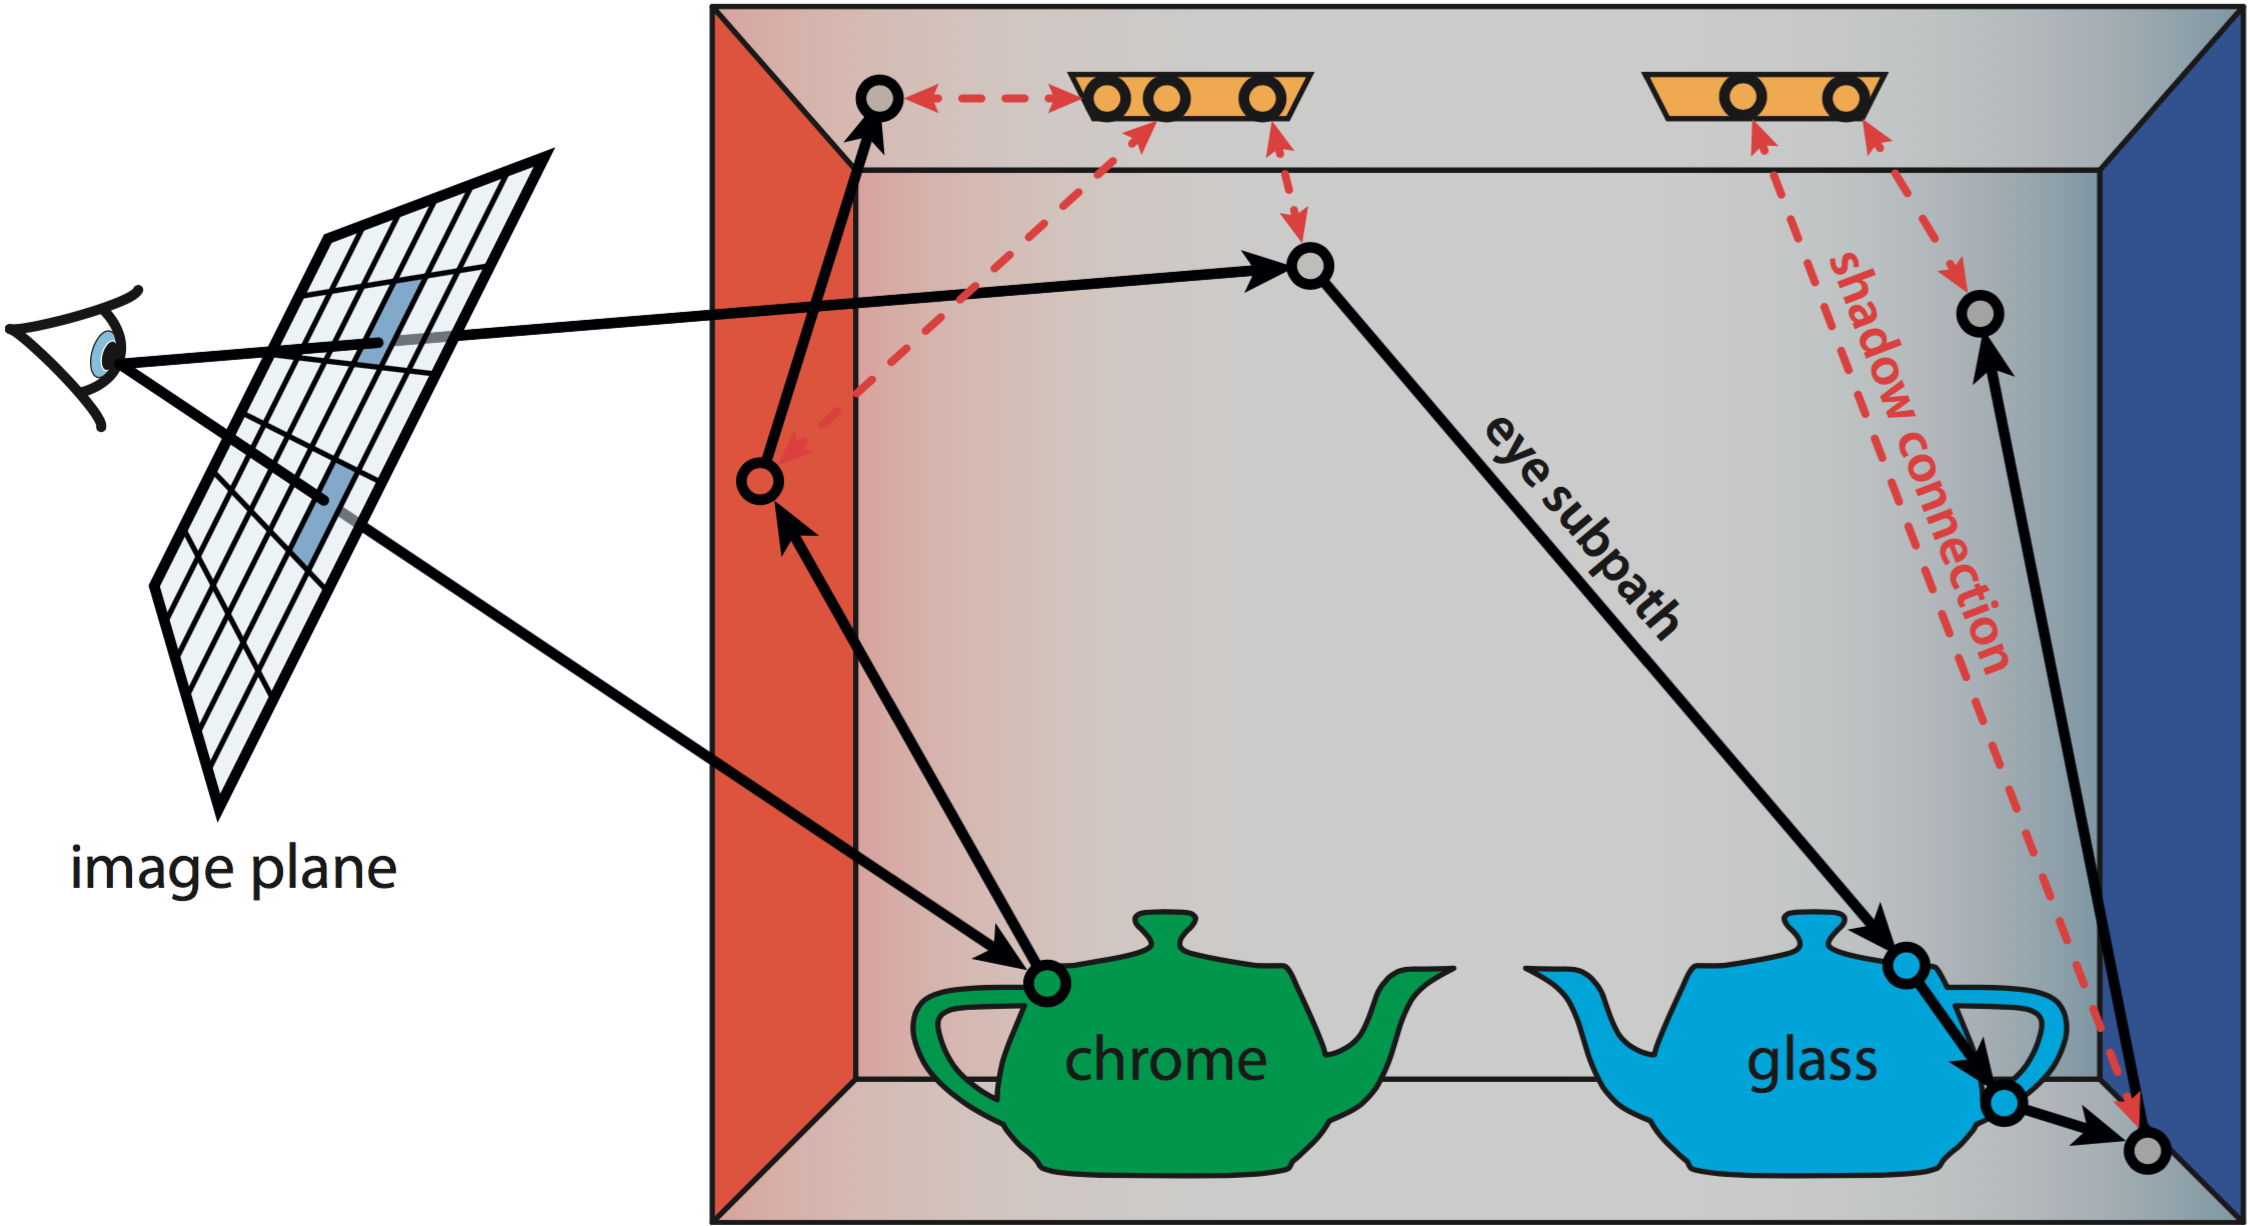
\includegraphics[width=1.0\textwidth]{figures/pt/direct-indirect}
	\caption{为了提升路径追踪算法的收敛速度及采样效率,路径追踪算法通常会在每个顶点引入直接光照,这通过从这些点发射阴影光线的方式来获得,这种方式并不会增加路径追踪估计的偏差(图片来自\cite{a:ThePathtoPath-TracedMovies})}
	\label{f:pt-shadow-rays}
\end{figure}

需要注意的是,直接光照的计算与路径的采样是不同的,它可能不止一个采样点,这是因为直接光照的采样并不会像间接路径那样无限递归下去,并且我们往往需要更精确的直接光照采样来达到更高的效率。但在采样的时候也需要注意重要性采样,首先是对于多个光源的场景,每个光源的采样数量应该正比于它对场景的相对贡献值,其次是每个光源内部不同部分的光照分布可能是不同,对每个光源内部的采样分布应该正比于其光照分布。

对于单个光源,其通常包含一个面积概率密度分布,我们可以直接使用该概率密度来对光源进行采样;对于多个光源,通常需要按照每个光源的重要度进行划分,以使贡献更大的光源获得更多的采样数量。关于直接光照的采样,它其实是一个对光源分布进行重要性采样的问题,更详细的内容可以参考\cite{b:AdvancedGlobalIllumination}。在本章的后面,我们还将看到一种用来处理焦散效果的特殊的直接光采样方法。






\subsubsection{基本路径采样}
虽然每个顶点的直接光照的采样可以有效地提升路径追踪的效率,但是对于高质量的图像,路径的采样方法却更加重要,路径采样的目标就是要找出那些对光照贡献很大的足够长度的间接光,这涉及非常多种不同的采样技术,这些不同的路径采样技术也是路径追踪技术研究的热门内容和方向,本节将会讨论基本的路径采样方法,在后面的内容中会介绍一些更高级的采样方法。

给定一个高维积分,蒙特卡洛方法的基本步骤是直接生成一个对应维度的向量随机数,然后直接将这些随机数带入蒙特卡洛估计中。然而在光照传输中却不能简单地这么做,首先光照传输中的被积函数的形式是隐藏在场景的表面分布当中的,尽管在式\ref{e:pt-path-form}中的被积函数中能够可以看出它们就是BRDF函数的乘积,但是它们实际上只是每个路径给定后的一个值,即是路径积分的被积函数是所有路径已知情况下的分布,因此,不管路径追踪算法采用何种采用技术,找出有效且重要的路径都是必不可少的;也正是路径的必要性,我们也不能直接从表面上随机选择一些顶点作为一条路径,因为这些路径可能是无效的,每个顶点之间还需要进行可见性测试。

所以路径追踪算法的前提是找到一条有效的路径,然后才是保证这条路径的重要性,每条路径的贡献越大,收敛速度可能越快,但是最终收敛速度还需要看找到每条有效路径的成本。

最传统的路径采样方法其实和分布式光线追踪是一样的,都是从摄像机这个其实顶点开始,然后按照光线传输以及其与表面的交互进行递归路径追踪,唯一不同的是路径追踪每一次与表面交互只产生一条新的光线,而分布式光线追踪产生多条新的方向的光线,形成一颗光线树。因此RenderMan\footnote{参见:\url{https://renderman.pixar.com/resources/current/RenderMan/pathTracing.html}}就同时提供两种选项给用户,路径追踪用于快速产生比较高准确度的图像供产品开发,但是分布式光线追踪主要用于产生最终高质量的产品。

\begin{figure}
\sidecaption
	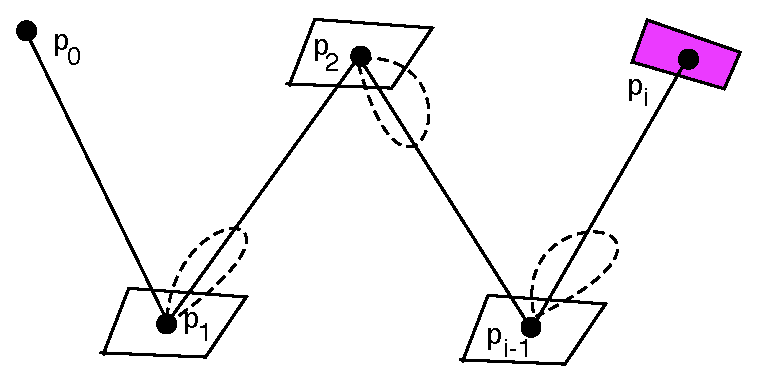
\includegraphics[width=0.6\textwidth]{figures/pt/path-tracing}
	\caption{为了获取更重要的路径,传统的路径采样主要是基于表面的BRDF反射分布来对反射或折射方向进行采样,如果对半空间均匀分布则会导致高光这样的重要分布采样几率变小从而收敛速度变慢}
	\label{f:pt-path-sampling}
\end{figure}

最基本的路径采样技术跟分布式光线追踪技术是类似的,一般是根据材质的BRDF函数分布来进行重要性采样,如图\ref{f:pt-path-sampling}所示,这样单次采样速度受BRDF函数复杂度的影响,另一些路径采样技术使用基于空间的均匀分布,这样收敛速度可能很慢,但是单次采样的速度很快。

一个基本的路径追踪算法的伪代码如下:

\begin{lstlisting}[language=C++]
Color TracePath(Ray r) {
	Color radiance = 0;
	if (!RussianRoulette()) {
    	r.FindNearestObject();
    	if (r.hitSomething == false) 
      		return Black;  // 没有交点,可能位于空间外

		//获取交点材质参数
    	Material m = r.thingHit->material;
    	Color emittance = m.emittance;

    	//根据某种路径采样方式获取一个随机方向
    	Ray newRay;
    	newRay.origin = r.pointWhereObjWasHit;
    	newRay.direction = RandomRayDirection(m);

    	//计算BRDF反射率
    	Color BRDF = ComputeBRDFAndTheta();
    	Color reflected = TracePath(newRay);
    	Color indirect = BRDF * reflected

    	//计算该点的最终光照,需要加入前面的直接光照项
    	radiance = emittance + indirect + DirectIllumination(r.origin);
    }
	return radiance;
}
\end{lstlisting}

注意此处我们并没有严格地考虑俄罗斯轮盘终止情况,它需要额外记录每个顶点处前面所有顶点BRDF反射率的乘积,以决定什么时候开始运用俄罗斯轮盘终止测试以及其导致的相应的概率处理,请参见前面的内容。







\subsection{双向路径追踪}\label{sec:bidirectional-path-tracing}
回顾一下到目前为止我们讨论的路径采样技术,它首先从摄像机出发,沿着屏幕区域发射一条随机的可视光线,然后求得该光线与场景表面的第一个交点,并获取该交点的材质信息,然后从该点材质中的BRDF反射分布函数抽取一条新的反射或折射光线,这条路径以这样的方式递归追踪,直到它与某个光源相交,或者满足某个终止条件追踪被终止,在该路径的每个顶点,为了使更快地获取足够的光照,直接光照被考虑,它通过直接向光源发射阴影光线来计算直接光源。这样形成的整条路径又称为摄像机路径(eye path)\myindex{摄像机路径}{eye path}。

摄像机路径的不足在于它对光源的采样严重不足,因为它完全依赖于每一个顶点处新的随机光线会击中某个光源,然而由于实际场景中通常光源占据很小的面积,使得摄像机路径击中光源的几率非常小,这大大抑制了估计的收敛速度。例如对于图\ref{f:pt-bid-tracing}这样的情况,光源发射出的光照通过很小的区域传递到整个场景,这个区域被采样的几率显然非常小,所以就会导致整个收敛速度非常慢。

\begin{figure}
\sidecaption
	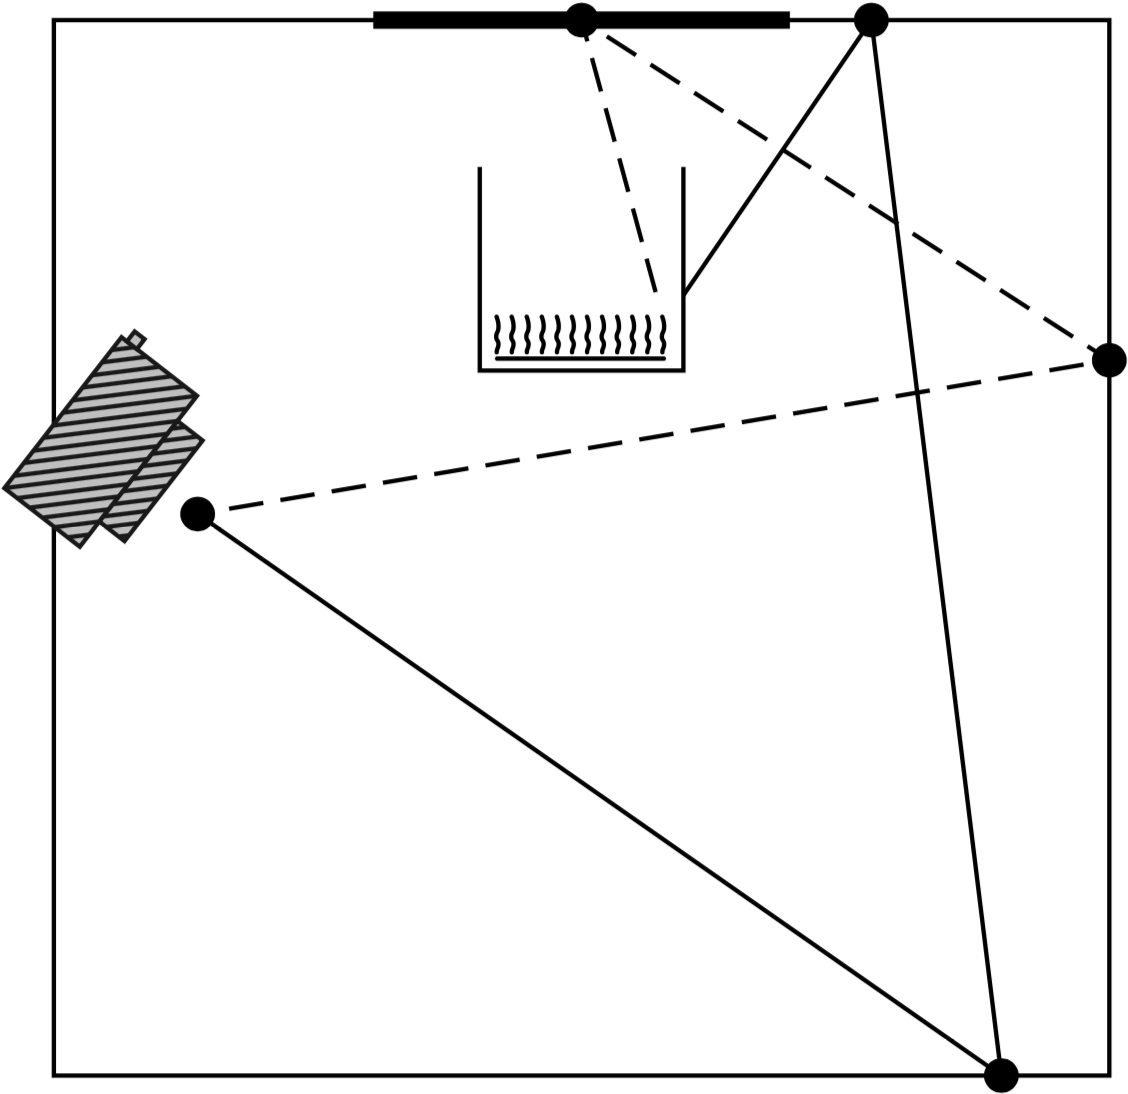
\includegraphics[width=.3\textwidth]{figures/pt/path-9}
	\caption{这里光源的光照通过很狭窄的区域传递到整个场景,传统的路径追踪算法会使得该区域被采样的几率非常小,从而导致大部分路径都不能有效地与光源相交,收敛速度大大降低}
	\label{f:pt-bid-tracing}
\end{figure}

这里需要注意的是,我们通过确定性方法选择的直接光照并不能有效提升收敛速度,直接光照带来的好处是在光线数量不多的时候可以更快地获取更多的光照信息,但是最终的图像质量要依赖于路径随机击中光源的贡献。为什么呢?因为根据顶点的BRDF分布,路径追踪的方向才是对每个顶点贡献更多光照的方向,直接光照仅仅对漫反射表面会提升收敛速度,但是对于高光表面,路径方向的光照可能是更重要的。

所以为了更好地对光源进行采样,一些算法使用相反的顺序,它们从光源出发,按正常的光线传输的方向向摄像机追踪,这种路径称为光源路径(light path)\myindex{光源路径}{light path}。然而光源路径又会带来对屏幕空间的采样不足,所以我们希望能够将这两种采样方式的优点结合起来,这就是双向路径追踪技术。

双向路径追踪(bidirectional path tracing)\myindex{双向路径追踪}{bidirectional path tracing}由\cite{a:Bi-directionalpathtracing}和\cite{a:BidirectionalEstimatorsforLightTransport}独立提出,它的核心思路就是将摄像机路径和光源路径结合起来,双向路径追踪算法有多种形式,例如光子映射,即时辐射度都是属于双向路径追踪算法,这里我们首先介绍它最基本的方法。

如图\ref{f:pt-bidirectional}所示,基本的双向路径追踪算法首先从摄像机和光源两个方向独立进行路径追踪,其结果形成一条由$y_0,y_1,\cdots,y_n$组成的从$y_0$出发的光源路径,以及一条由$x_m,x_{m-1},\cdots,x_0$组成的终点$x_0$落在摄像机上的摄像机路径,为了形成一条完整的路径,我们将两条路径的终点$y_n$和$x_m$连接起来,形成一条长度为$m+n+1$的完整路径,当然$y_n$和$x_m$是可能被其他物体遮挡的,所以它们需要进行可见性测试,这形成一条阴影路径,如图\ref{f:pt-bidirectional}中的虚线路径。

\begin{figure}
	\sidecaption
	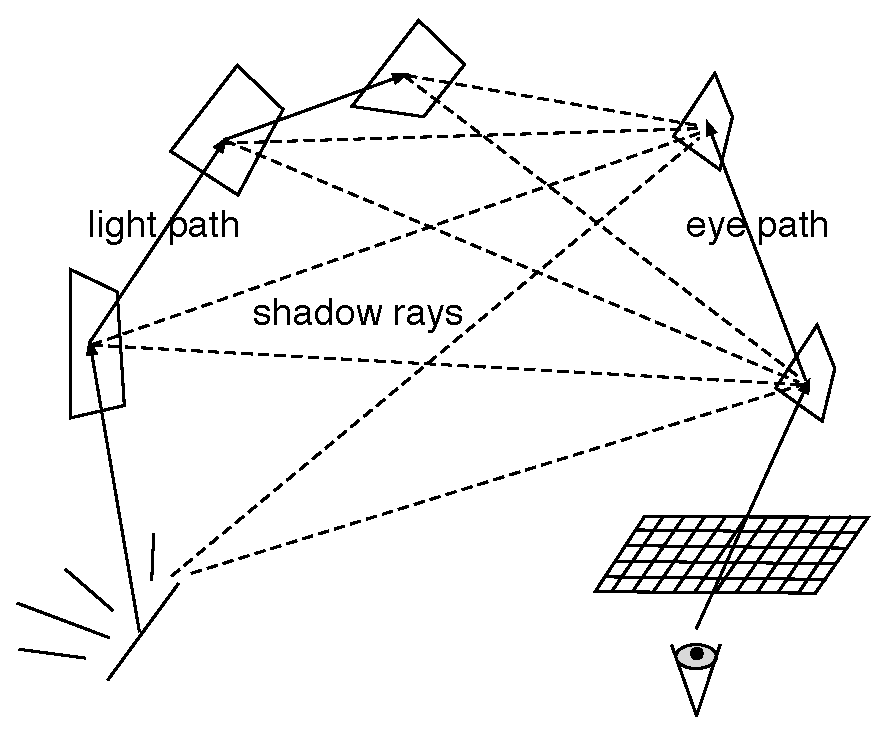
\includegraphics[width=0.5\textwidth]{figures/pt/bidirectional}
	\caption{双向路径追踪首先分别从摄像机和光源构建两条子路径,然后使用阴影光线将两条自路径中的所有顶点连接起来,连接后的每条完整的概率由复合重要性采样的平衡启发式决定}
	\label{f:pt-bidirectional}
\end{figure}

摄像机路径和光源路径可以看做是对光照贡献在定义域上的一种分割(partitioning),它们分别使用符合各自对应部分的特征,因此我们可以使用复合重要性采样的方式将这两者结合起来,即我们在将$y_n$和$x_m$连接成一条完整路径的时候,该完整路径的概率由上一章讨论的复合重要性采样的平衡启发式(balance heuristic)\myindex{平衡启发式}{balance heuristic}计算而得(参见第\ref{sec:mc-balance-heuristic}节的内容)。

实际上双向路径追踪还有一个意外的好处,即我们不仅可以连接$y_n$和$x_m$形成一条完整的路径,还可以分别连接两条子路径上所有的点形成更多的路径,并且这些路径上的点只需要追踪一次,它们的纹理查询及着色计算也只需要计算一次,这将大大加快估计的收敛速度,如图\ref{f:pt-bidirectional}所示。

传统路径追踪和双向路径追踪的比较可以参见图\ref{f:pt-bid-tracing-show},双向路径追踪算法的收敛速度会大大快于传统的路径追踪。

\begin{figure}
\sidecaption
	{\begin{subfigure}[b]{0.31\textwidth}
		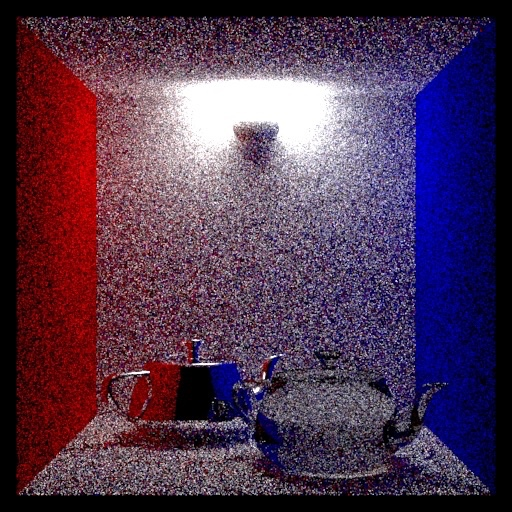
\includegraphics[width=1.0\textwidth]{figures/pt/path-8-1}
		\caption{单向(2048 spp)}
	\end{subfigure}
	\begin{subfigure}[b]{0.31\textwidth}
		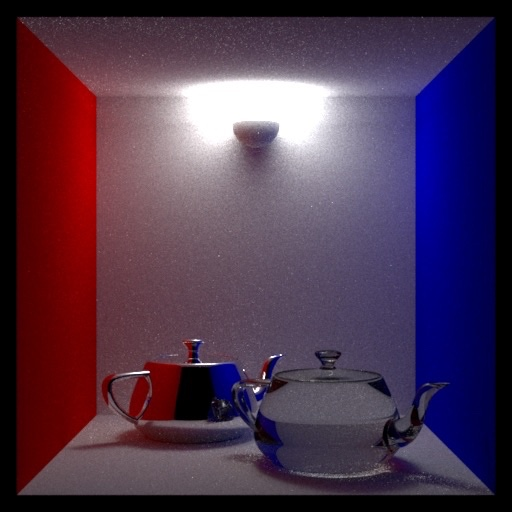
\includegraphics[width=1.0\textwidth]{figures/pt/path-8-2}
		\caption{双向(600 spp)}
	\end{subfigure}
	}
	\caption{传统路径追踪对光源的采样不够导致大部分光线对光照的贡献都很小,因此收敛速度非常慢,双向路径追踪使用复合重要性采样来分别摄像机和光源进行重要性采样,使得收敛速度大大加快(图片来自\cite{a:PathtracinginRenderMan})}
	\label{f:pt-bid-tracing-show}
\end{figure}

尽管双向路径追踪能够复合对光源和屏幕区域进行重要性采样,然而由于每个完整的路径都是通过阴影光线连接的,如图\ref{f:pt-bidirectional}所示,阴影光线本身是很可能被阻挡的,并且阴影光线和直接光照一样,它的贡献可能会大大小于针对BRDF进行重要性采样的方向的光照贡献,这使得联合后的完整路径的贡献也随之降低。我们将在下一章看到一些提升双向路径算法组合的路径的光照贡献的方法。







\section{纹理过滤}\label{sec:pt-texture-filtering}
到目前为止,我们理解了路径追踪算法的基本思路,它主要是基于蒙特卡洛方法,对路径空间进行采样产生一些随机数(路径),然后使用这些随机数加权平均来近似图像颜色分布。这里每条路径是一个随机数,它是对路径空间进行采样的结果。对于任何采样发生的地方,走样问题几乎总是存在,理论上,路径追踪算法中的走样都可以通过对路径进行超采样(super sampling)\myindex{超采样}{super sampling}来消除,然而由于每条路径采样的计算成本非常高,因此实践中通常还要结合其他一些方法来实现反走样。本节我们就将讨论一种路径追踪算法中比较流行的反走样技术,即对纹理采样进行过滤。

\begin{figure}
	\sidecaption
	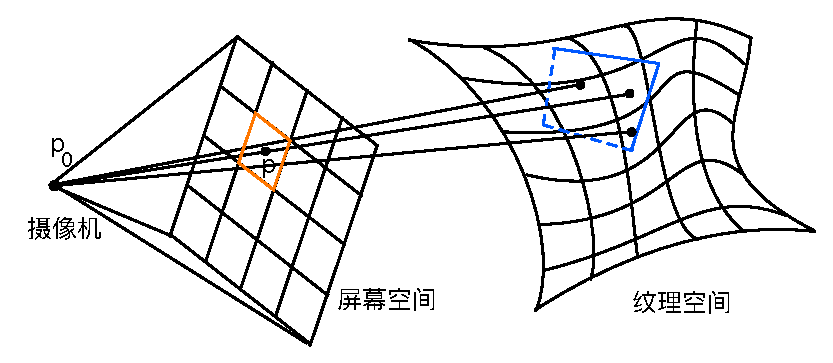
\includegraphics[width=0.6\textwidth]{figures/pt/filter-size}
	\caption{渲染算法计算的是一个像素区域的颜色,这个区域投射到路径与表面的交点处形成较大面积的足迹,这就需要使用更高的采样率才能够有效消除由采样不足导致的噪点,这意味着每个像素需要发射更多的光线,大大降低了渲染效率}
	\label{f:pt-filter-size}
\end{figure}

在渲染算法最终生成的图像上,每个像素的颜色是由该像素区域投射到场景的一个四边形区域决定的,该四边形区域称为光线的足迹(footprint),如图\ref{f:pt-filter-size}所示。随着路径长度的不断增加,这个足迹的面积可能会随着光线的直线传播\footnote{例如两个不平行的光的直线传播会导致相互的距离越来越大,从而投射面积越来越大。}以及在表面的散射等发生变化。当纹理被作用于路径的每个顶点的着色计算时,即是需要对纹理进行采样,如果采样率过小就会导致采样不足形成走样的图像(aliased image)\myindex{走样的图像}{aliased image},传统的做法是使用超采样技术对每个像素发射多条光线然后对这些光线进行过滤来进行反走样,这样使得远处较大面积的足迹区域能够获得更高的采样率,由于光线追踪算法中每条光线的计算成本都非常高,通过超采样来消除纹理走样(texture aliasing)\myindex{纹理走样}{texture aliasing}的计算效率很低,因此更有效的反走样方法是直接对纹理采样的过程进行反走样处理。

反走样(anti-aliasing)\myindex{反走样}{anti-aliasing}技术的核心思路就是过滤,它将某个位置的函数值与周围一定范围内的函数值按照一定的权重进行混合,这样就使得采样结果更平滑\footnote{过滤的本质实际上是移除过高的频率。},有效地消除了走样。过滤技术通常涉及使用一个范围权重分布函数$h(p)$与采样结果的卷积计算(参见第1章的内容),这个范围权重分布函数对一定范围内的每个采样点分配一个权重值进行混合,超出这个范围的权重为0,这个范围越大,则过滤结果越模糊,反之则越尖锐。所以纹理过滤的关键是找到每条光线在传播过程中每一个顶点处足迹的尺寸。

在传统的基于光栅化的渲染算法中,它并不直接计算一条光线的传输过程,而是直接计算摄像机看到的场景中的点的着色,即直接光源,所有其他全局光照效果则通过一些间接的方法来计算,所以我们总是能通过摄像机投影矩阵以及这些点的深度值来计算每个像素范围投射在表面上的面积,这个面积可以用来帮助选择多级纹理(mipmap)\myindex{多级纹理}{mipmap}的层级。多级纹理的层级实际上反应的就是过滤函数的范围,因为如果一个函数的采样率太低,则中间的很多重要信息可能直接被忽略,多级纹理从$0$级逐渐减小采样率,$n+1$级纹理直接在第$n$级纹理基础上采样,这样实际上就是在扩大低级纹理的过滤范围,因为直接使用过大的过滤范围会影响计算性能,所以多级纹理实际上是对大范围过滤的一种预计算。

然而在光线追踪算法中,我们需要对一条光线路径上每个顶点进行着色计算,所有二次以上反弹的顶点的着色计算并不能简单地使用它与摄像机的距离(即深度)来决定纹理过滤范围,因为正确的过滤范围是从摄像机看上去一条路径上每个顶点对应的足迹是多大,这个足迹会随着光线的传输,与表面的交互等进行变化。

所以,在光线追踪算法中,为了有效地对纹理进行过滤,我们需要计算每条路径中每个顶点处的足迹,这正是本节要讨论的内容。虽然存在一些并不需要跟踪整个光线足迹的局部过滤方法,但是这些方法往往无法满足高质量的需求。所以本节我们仅讨论几种跟踪计算整体路径足迹的纹理过滤方法。






\subsection{光线微分}\label{sec:pt-ray-differentials}
光线追踪算法中每条光线会在场景中多次反弹最终进入光源或者摄像机,在这个过程中每一个光与表面相交的顶点都需要对纹理进行采样,因此我们要计算光线在传播过程中经过的每一个路径顶点的足迹。早期的一些方法如\cite{a:Beamtracingpolygonalobjects,a:RayTracingwithCones,a:Principlesandappli-cationsofpenciltracing}通过发射一束(而不是单条)光线,并使用整束光线的覆盖范围来计算光线的足迹,然而这样的光束却很容易在与表面的反射或折射等交互中发散,使得足迹的计算非常困难。

\cite{a:TracingRayDifferentials}提出的光线微分(ray differential)\myindex{光线微分}{ray differential}是一种非常简单而有效的方法,它对每条中心光线(central ray)\myindex{中心光线}{central ray}在屏幕上$x$和$y$方向分别偏移1个像素以产生两条光线微分,然后让这两条光线微分随着中心光线一起在场景中传播,在路径的每个顶点处,该光线微分与表面的交点同中心光线交点的距离用来近似该顶点的足迹。光线微分是目前工业中使用比较广泛的方法,例如PBRT\cite{b:pbrt}和Pixar的RenderMan\cite{a:RayDifferentialsandMultiresolutionGeometryCachingforDistributionRayTracinginComplexScenes}均使用光线微分来对纹理进行过滤。

通过前面的分析,要想计算光线路径中某个顶点足迹的大小,我们需要将一个像素的尺寸通过该路径投射到该顶点所在的表面上,因此这个足迹必须可以表示为屏幕坐标空间$x$和$y$的函数,这正是光线微分方法的基本出发点。光线追踪算法可以看做是一系列对一条包含一个原点位置和方向的光线的操作,而一条从摄像机出发的起始光线可以表示为屏幕坐标空间$x$和$y$的函数,因此经过一系列变换操作后,所有可以通过这条路径上的光线计算的量,如表面的纹理坐标等,都可以表述为屏幕空间$x$和$y$的函数:

\begin{equation}
	v=f_n(f_{n-1}(\cdots f_2(f_1(x,y))))
\end{equation}

\noindent 因此只要能够计算这些对光线的操作函数$f_n$,就能够计算每个顶点的足迹。

以下我们介绍光线微分方法的原理,这里加粗的字母表示位置或方向矢量,否则为标量。首先,一条光线可以表述为一个表示位置的点和一个表示方向的单位矢量的组合:

\begin{equation}
	\overrightarrow{\mathbf{R}}=\langle \mathbf{P} \text{ }\mathbf{D}\rangle
\end{equation}

\noindent 初始的摄像机光线可以由图像平面坐标系表示:光线的起始位置就是摄像机位置,摄像机的朝向为观察方向,所以一个由摄像机穿过一个像素的光线的方向可以表示为观察方向在图像平面上的偏移:

\begin{equation}
	\mathbf{d}(x,y)=\mathbf{View}+x\mathbf{Right}+y\mathbf{Up}
\end{equation}

\noindent 所以初始摄像机光线可以表示为:

\begin{equation}
	\begin{aligned}
		\mathbf{P}(x,y)&=\mathbf{Eye}\\
		\mathbf{D}(x,y)&= \cfrac{\mathbf{d}}{(\mathbf{d}\cdot \mathbf{d})^{1/2}}
	\end{aligned}
\end{equation}

因此一条光线被表示为屏幕空间的一个函数,所以后面所有需要通过光线来求得的度量都可以表示为屏幕空间的函数。 为了计算每个顶点的足迹,这里对每条光线沿屏幕空间$x$方向和$y$方向产生一个像素的偏移,以产生一对光线微分:

\begin{equation}
	\begin{aligned}
		 \cfrac{{\rm \partial}\overrightarrow{\mathbf{R}}}{{\rm \partial} x}&=\bigg\langle  \cfrac{{\rm \partial}\mathbf{P}}{{\rm \partial} x} \text{ } \cfrac{{\rm \partial}\mathbf{D}}{{\rm \partial} x}\bigg\rangle \\
		 \cfrac{{\rm \partial}\overrightarrow{\mathbf{R}}}{{\rm \partial} y}&=\bigg\langle  \cfrac{{\rm \partial}\mathbf{P}}{{\rm \partial} y} \text{ } \cfrac{{\rm \partial}\mathbf{D}}{{\rm \partial} y}\bigg\rangle
	\end{aligned}
\end{equation}

那么光线微分表示的是一个什么量?在数学上微分表示的是函数的局部变化,所以它表示的是两条光线之间的差,如图\ref{f:pt-ray-differentials}所示,所以光线的位置分量的微分$ \cfrac{{\rm \partial}\mathbf{P}}{{\rm \partial} x}$和$ \cfrac{{\rm \partial}\mathbf{P}}{{\rm \partial} y}$就能够表示每个顶点的足迹。

\begin{figure}
	\sidecaption
	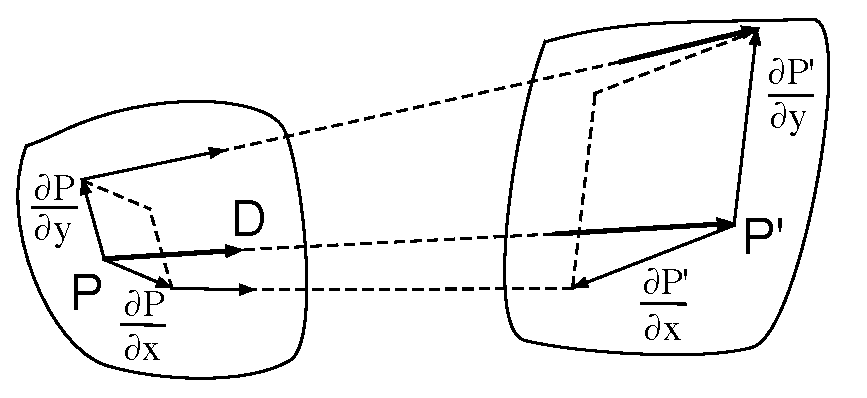
\includegraphics[width=0.55\textwidth]{figures/pt/ray-differentials}
	\caption{对每个中心光线发射两条额外的偏移光线,并让它们跟随中心光线一起传播,在每个顶点出求得所有光线的位置,就能够利用泰勒展开式来近似位置微分,即是顶点的足迹}
	\label{f:pt-ray-differentials}
\end{figure}

那么应该怎样求这个位置微分呢,这里实际上需要用到一阶泰勒近似(first-order Taylor approximation)\myindex{一阶泰勒近似}{first-order Taylor approximation},即:

\begin{equation}\label{e:pt-first-order-taylor}
	\begin{aligned}
		\mathbf{P}^{'}(x+\Delta x,y)-\mathbf{P}(x,y)& \approx\Delta x \cfrac{{\rm \partial}\mathbf{P}}{{\rm \partial} x}\\
		\mathbf{P}^{'}(x,y+\Delta y)-\mathbf{P}(x,y)& \approx\Delta y \cfrac{{\rm \partial}\mathbf{P}}{{\rm \partial} y}\\
	\end{aligned}
\end{equation}

这个过程在程序中是怎么实现的呢?首先我们对每条中心光线沿$x$和$y$方向各自偏移1像素产生两条额外的光线,然后这两条光线微分跟着中心光线一起传播,当中心光线和表面相交于$\mathbf{P}^{'}$点时,我们同时求出两条光线微分与表面的交点位置,如图\ref{f:pt-ray-differentials}所示,最后利用式\ref{e:pt-first-order-taylor}求出足迹的大小。

实际上光线微分是要计算的最终值,而不是两条额外光线的度量,我们需要用一条光线(具有位置和方向)而不是一个光线微分(两条光线之差)来描述这两条额外光线,所以为了描述简便,在概念上我们有时用光线微分来泛指两条偏移的光线,例如PBRT\cite{b:pbrt}中光线微分的数据结构定义如下:

\begin{lstlisting}[language=C++]
class RayDifferential : public Ray { 
public:
	Point3f rxOrigin, ryOrigin;
	Vector3f rxDirection, ryDirection;
};
\end{lstlisting}

那应该怎样计算光线微分与表面的交点?如果我们仍然像中心光线一样进行光线-表面相交测试,就会导致很大的计算成本,并且它又会出现和前面其他光束类方法的问题。为了简化光线微分的传播,光线微分技术的一个重要基础是假设交点表面是镜面的,这样我们只需要对中心光线进行一次相交测试并求出相交面的隐式函数,就可以通过数学方法计算出两条光线微分的交点,我们把这个计算过程放入到后面的传输操作中。






\subsubsection{光线微分的传播}
有了对光线微分的表述形式,接下来就需要计算这两条光线微分的传播过程,如前面所述,只要计算出光线微分在每个顶点处的交点,就可以计算出它们与中心光线的真正的微分,即两条光线只差,它们最终用于光线足迹的计算。

光线微分技术的核心假设是镜面反射平面,在光线与镜面的交互过程中,有三种情况会修改光线,它们分别是光线的直线传输,反射和折射,这三种操作每个都可以看做是一个作用于$(x,y)$的函数,通过它们就可以计算出光线路径中每个顶点处光线微分与表面的交点。

在光线追踪算法中,光线(ray)实际上是一个静态的量,它仅是一个特定点和特定方向的组合,或者我们认为它是一个具有方向的“点”,这个点可以随着该光线的方向沿直线传播,但是光线定义本身并不包含这个动态的传播过程,传播过程中的每一个“点”都是一条新的光线,例如PBRT中光线类的定义如下:

\begin{lstlisting}[language=C++]
class Ray {
public:
    Point3f o;
    Vector3f d;
}
\end{lstlisting}

所以光线在路径中由一个顶点传输到另一个顶点的过程,如图\ref{f:pt-ray-differentials}所示,其实就是沿光线的方向移动光线的过程,使用参数$t$来表示移动的距离,则新的光线的可以由下式计算而出:

\begin{equation}
\begin{aligned}
	\mathbf{P}^{'}&=\mathbf{P}+t\mathbf{D}\\
	\mathbf{D}^{'}&=\mathbf{D}
\end{aligned}
\end{equation}

\noindent 因此当中心光线传输距离$t$之后,其对应的两条偏移的光线可以由以下式计算出光线微分(这里仅列出沿$x$方向偏移的光线):

\begin{equation}\label{e:pt-ray-transfer}
	\begin{aligned}
		 \cfrac{{\rm \partial}\mathbf{P}^{'}}{{\rm \partial} x}&=( \cfrac{{\rm \partial}\mathbf{P}}{{\rm \partial} x} +t \cfrac{{\rm \partial}\mathbf{D}}{{\rm \partial} x})+ \cfrac{{\rm \partial} t}{{\rm \partial} x}\mathbf{D} \\
		 \cfrac{{\rm \partial}\mathbf{D}^{'}}{{\rm \partial} y}&=  \cfrac{{\rm \partial}\mathbf{D}}{{\rm \partial} y}
	\end{aligned}
\end{equation}

\noindent 我们已经知道$\mathbf{P}$点处的光线微分$ \cfrac{{\rm \partial}\mathbf{P}}{{\rm \partial} x}$和$ \cfrac{{\rm \partial}\mathbf{D}}{{\rm \partial} y}$的值,这里需要计算$t$的值以及$ \cfrac{{\rm \partial} t}{{\rm \partial} x}$的值。

对于中心光线与表面的交点$\mathbf{P}^{'}$是通过光线-表面相交测试计算出的,那么在不进行相交测试的情况下,怎样计算出两条光线微分的与表面的相交位置呢?这里正是光线微分技术简化光线足迹计算的前提:即假设在光线足迹的尺寸内,光线微分和中心光线与表面的交点是位于同一个平面的,即中心光线交点处表面的切面。这样我们通过中心光线与表面的相交计算就能够提取出该正切平面的隐式函数,然后将光线函数代入这个平面的隐式函数就可以使用数学方法(而不是相交计算)计算出$t$的值。因此这也是光线微分技术的限制,它只能处理绝对光线的镜面。

一个平面的隐式函数可以由下式给出:

\begin{equation}
	ax+by+cz+d=0
\end{equation}

\noindent 这里$\mathbf{N}=(a,b,c)$表示中心光线与表面交点处(即$\mathbf{P}^{'}$)的法线,将光线传输函数$r(t)=\mathbf{P}+t\mathbf{D}$代入上式,即可以计算出$t$的值为:

\begin{equation}
	t= \cfrac{-\mathbf{N}\cdot \mathbf{P}-d}{\mathbf{N}\cdot\mathbf{D}}
\end{equation}

\noindent  为了计算两条光线微分的$t$值,我们首先需要计算出平面隐式函数中的$d$值。这是通过中心光线来计算的,因为中心光线的相交计算会得到中心光线与表面相交的$t$值,将中心光线的$t$值代入上式就可以求出平面隐式函数中的$d$值,然后在给定两条光线微分的起点位置和方向的情况下,就可以求出两条光线微分与同一平面相交对应的$t$值。

\noindent 最终我们可以得到光线微分$t$值的微分为:

\begin{equation}
	 \cfrac{{\rm \partial} t}{{\rm \partial} x}=- \cfrac{( \cfrac{{\rm \partial}\mathbf{P}}{{\rm \partial} x} +t \cfrac{{\rm \partial}\mathbf{D}}{{\rm \partial} x})\cdot\mathbf{N}}{\mathbf{D}\cdot\mathbf{N}}
\end{equation}

注意在上式的证明过程中,假设$\mathbf{N}$是和$t$无关的,因为偏移光线和中心光线位于同一个平面上,它们的法线不变,所以这里$\mathbf{N}$是一个“常量”,只需要对$\mathbf{P}^{'}=\mathbf{P}+t\mathbf{D}$求偏导数。尽管上式是基于平面推导出的,\cite{a:TracingRayDifferentials}说明该式对于任意曲面都是成立的,因为在极限情况下,偏移光线会越来越接近于中心光线,它们的交点所在的平面接近于一个平面,所以偏移光线的交点处于中心光线交点的正切面上。

参考\cite{a:TracingRayDifferentials}的原论文,光线微分的反射可以由以下式推导出:

\begin{equation}
	\begin{aligned}
		 \cfrac{{\rm \partial}\mathbf{P}^{'}}{{\rm \partial} x}&= \cfrac{{\rm \partial}\mathbf{P}}{{\rm \partial} x}\\
		 \cfrac{{\rm \partial}\mathbf{D}^{'}}{{\rm \partial} x}&= \cfrac{{\rm \partial}\mathbf{D}}{{\rm \partial} x}-2\Bigg[\bigg(\mathbf{D}\cdot\mathbf{N}\bigg) \cfrac{{\rm \partial}\mathbf{N}}{{\rm \partial} x}+ \cfrac{{\rm \partial} (\mathbf{D}\cdot\mathbf{N})}{{\rm \partial} x}\mathbf{N}\Bigg]
	\end{aligned}
\end{equation}

\noindent 其中:

\begin{equation}
	 \cfrac{{\rm \partial} (\mathbf{D}\cdot\mathbf{N})}{{\rm \partial} x}= \cfrac{{\rm \partial}\mathbf{D}}{{\rm \partial} x}\cdot\mathbf{N}+\mathbf{D}\cdot \cfrac{{\rm \partial}\mathbf{N}}{{\rm \partial} x}
\end{equation}

\noindent 折射的光线微分为(这里$\eta$为折射率比率):

\begin{equation}
	\begin{aligned}
		 \cfrac{{\rm \partial}\mathbf{P}^{'}}{{\rm \partial} x}&= \cfrac{{\rm \partial}\mathbf{P}}{{\rm \partial} x}\\
		 \cfrac{{\rm \partial}\mathbf{D}^{'}}{{\rm \partial} x}&=\eta \cfrac{{\rm \partial}\mathbf{D}}{{\rm \partial} x}-\bigg(\eta \cfrac{{\rm \partial}\mathbf{N}}{{\rm \partial} x}+ \cfrac{{\rm \partial}\mu }{{\rm \partial} x}\mathbf{N}\bigg)
	\end{aligned}
\end{equation}

\noindent 其中

\begin{equation}
	 \cfrac{{\rm \partial}\mu }{{\rm \partial} x}=\Bigg[ \eta- \cfrac{\eta^{2}(\mathbf{D}\cdot\mathbf{N})}{(\mathbf{D}^{'}\cdot\mathbf{N})} \Bigg] \cfrac{{\rm \partial} (\mathbf{D}\cdot\mathbf{N})}{{\rm \partial} x}
\end{equation}

\noindent 这些偏移光线的传播过程(包括直线传输,反射和折射)中的微分计算公式看起来很复杂,然而我们重点是要把握它们的计算思路:

\begin{itemize}
	\item 首先我们已知$\mathbf{P}$点处三条光线$\overrightarrow{\mathbf{R}}$,$\overrightarrow{\mathbf{R}}_x$即$\overrightarrow{\mathbf{R}}_y$的值(即它们的起始点和方向),由此我们可以求出$\mathbf{P}$点处的微分值$ \cfrac{{\rm \partial}\mathbf{P}}{{\rm \partial} x}$和$ \cfrac{{\rm \partial}\mathbf{D}}{{\rm \partial} x}$。
	\item 当光线由$\mathbf{P}$传输到$\mathbf{P}^{'}$时,我们首先通过中心光线的相交计算出$\mathbf{P}^{'}$处正切面的隐式函数,然后通过微积分方法计算出两条光线微分的交点,并由式\ref{e:pt-ray-transfer}计算$\mathbf{P}^{'}$点处的微分值$ \cfrac{{\rm \partial}\mathbf{P}^{'}}{{\rm \partial} x}$和$ \cfrac{{\rm \partial}\mathbf{D}^{'}}{{\rm \partial} x}$,这两个值又成为后面反射和折射计算中的$ \cfrac{{\rm \partial}\mathbf{P}}{{\rm \partial} x}$和$ \cfrac{{\rm \partial}\mathbf{D}}{{\rm \partial} x}$值。
	\item 然后在反射和折射中,新引入的量为$ \cfrac{{\rm \partial} \mathbf{N}}{{\rm \partial} x}$,我们马上分析这个量。
\end{itemize}

在上述第二步中虽然假设三条光线的交点都处于同一平面,但是对于反射和折射,法线随表面的变化可能对足迹的传播有较大影响,因此在计算反射和折射时需要考虑法线的变化。如果表面是参数化的形式,则法线微分可以通过公式计算而出,对于我们常用的三角形网格表述的表面,三角形内每个点处的法线是插值的结果,\cite{a:TracingRayDifferentials}解释了法线微分的计算过程:首先中心光线的交点$\mathbf{P}$是其所在三角形三个顶点的线性组合,而显然$\mathbf{P}$点处的法线$\mathbf{N}_p$是$\mathbf{P}$的函数,所以最终$ \cfrac{{\rm \partial} \mathbf{N}}{{\rm \partial} x}$是能够通过$ \cfrac{{\rm \partial} \mathbf{P}}{{\rm \partial} x}$以及三角形三个顶点的参数计算而出的,如图\ref{f:pt-mapping}所示。所以通常的做法是,在计算$\mathbf{P}$与表面的交点时,由于此时已经获取到三角形的三个顶点以及$\mathbf{P}$点的参数形式,所以此时可以直接计算出$\mathbf{P}$点出的法线偏导数$ \cfrac{{\rm \partial} \mathbf{N}}{{\rm \partial} x}$,然后在计算偏移光线的时候,直接代入$\Delta\mathbf{P}$即可,读者可参考PBRT\footnote{PBRT在计算交点$\mathbf{P}$时即计算出$dndu$和$dndv$两个变量,然后计算法线微分时直接代入位置变化$\Delta\mathbf{P}$即可。}中的实现。

\begin{figure}
	\sidecaption
	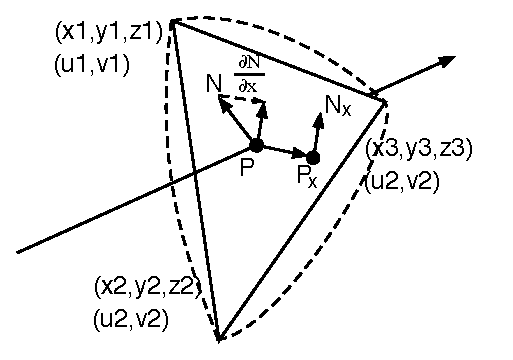
\includegraphics[width=0.5\textwidth]{figures/pt/mapping}
	\caption{在三角形表述的几何网格中,每条光线与表面的相交是通过找出与其相交的三角形来计算交点的,该三角形的三个顶点决定了该交点的参数形式,同样可由此计算出法线的偏导数}
	\label{f:pt-mapping}
\end{figure}



需要注意的是,这里计算出的$ \cfrac{{\rm \partial} \mathbf{P}}{{\rm \partial} x}$只是基于屏幕空间尺寸的足迹大小,表面本身的纹理采样函数包含有由屏幕空间向纹理空间转换的函数$\mathbf{T}(u,v)=f(\mathbf{p}(x,y))$,通过这个坐标空间转换的足迹才是最终用于纹理采样的足迹。纹理采样函数可以基于该足迹来选择多级纹理的层级,以及使用其他特定的过滤方法,关于这方面更详细的内容可以参考PBRT\cite{b:pbrt}第10章的内容。

虽然光线微分技术主要用于镜面反射,但是PBRT同时将光线微分技术用于所有摄像机光线,即直接光照部分的顶点的纹理采样,因为虽然它们的表面可能不是镜面的,但是其足迹大小可以被光线微分很好的近似,并且直接光照对走样的影响更大。

光线微分技术除了被用于纹理过滤,Pixar\cite{a:RayDifferentialsandMultiresolutionGeometryCachingforDistributionRayTracinginComplexScenes,a:RayTracingfortheMovieCars}还将其用于几何细分的选择,根据足迹的大小动态选择网格的精度。他们将光线分为两类,对于连贯性(coherence)非常好的光线(例如阴影光线,直接光,点光源等)选择高精度的网格,由于这类光线往往只需要与场景中很小一部分表面相交,因此只需要缓存很小一部分高精度的网格,占用缓存很小;对于一些很发散的光线,它们往往需要访问很大范围的网格数据,因此使用比较粗糙的网格数据,这样虽然网格所占据的场景范围很大,但是其总的网格数据却很小。通过这样的区分,更复杂的场景可以被更高效的计算。








\subsection{路径微分}\label{sec:pt-path-differentials}
在光线微分技术中,因为仅考虑镜面表面,光线与表面的交互(即反射或折射)仅由反射定律和折射定理决定,因此我们只需要知道初始光线在屏幕空间的坐标,即可以计算光线在场景中传播,即每条光线路径仅由屏幕空间坐标$(x,y)$决定。这样光线微分算法发射两条偏移光线并和中心光线一起在场景中传播,在每个顶点处就可以计算出偏移光线和中心光线的位置微分,这个微分被用于估计该顶点处的足迹。

虽然镜面表面的假设简化了光线微分的计算,然而它也限制了光线微分的使用:不能作用于光泽表面和漫反射表面。于是\cite{a:Pathdifferentialsandapplications}在光线微分的基础上将其扩展至任意表面。

光线微分技术在计算光线的反射或折射时,光线新的方向由反射和折射定理计算而出,因此在光线的传播过程中不会增加新的影响足迹传播的量。然而,为了支持非镜面表面,光线的反射或折射方向同时由当前光线和对另一个函数(例如BRDF或光源分布)进行采样来获得,这样光线微分就会同时受屏幕空间$(x,y)$以及其他所有参与方向采样的变量的影响。如图\ref{f:pt-path-differentials}所示,镜面反射的光线为$\mathbf{R}$,但是由于BRDF分布的影响,新的反射方向应该为$\mathbf{D}$,设BRDF分布可以由两个随机变量$(x_j)$和$y_j$($j$表示路径上第$j$个顶点)采样获得,那么光线微分将由$ \cfrac{\mathbf{D}^{'}}{{\rm \partial} x_j,y_j}$和$ \cfrac{\mathbf{D}^{'}}{{\rm \partial} x,y}$共同决定。

\begin{figure}
	\sidecaption
	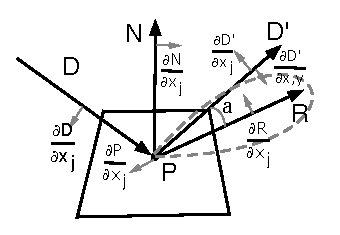
\includegraphics[width=0.45\textwidth]{figures/pt/path-differentials}
	\caption{在光线微分的基础上,路径微分通过对某种方向分布函数(如BRDF分布)进行采样来计算反射或折射方向,因此对光线的传播引入新的变量,光线微分需要由所有变量分量的偏导数共同决定}
	\label{f:pt-path-differentials}
\end{figure}


我们将新的方向$\mathbf{D}^{'}$的采样函数写为如下形式:

\begin{equation}
	\mathbf{D}^{'}=h(\mathbf{D},\mathbf{P},x,y)
\end{equation}

\noindent 其中,$x,y$为两个新引入的变量,则我们可以写出两个新变量的微分形式,它们连同$\mathbf{D}$和$\mathbf{P}$的微分(已知的),就可以求出$\mathbf{D}^{'}$的各个分量的偏导数,然后就可以求出每个偏移光线的微分。假设对于路径中的某个顶点$\mathbf{P}$有:

\begin{equation}
	\mathbf{P}=g(x_1,x_2,\cdots, x_k)=g_(X_k)
\end{equation}

\noindent 这里$g$称为路径生成函数(path generation function)\myindex{路径生成函数}{path generation function},$k$为顶点$\mathbf{P}$依赖的变量的数量。假设每个变量分量的微分为$\Delta x_j$,则该点的位置微分可由以下一阶泰勒近似计算:

\begin{equation}\label{e:pt-differential-vector}
	\Delta\mathbf{P}\approx\sum^{k}_{j=1}  \cfrac{{\rm \partial} g(x_1,x_2,\cdots, x_k)}{{\rm \partial} x_j}\Delta x_j
\end{equation}

\noindent 我们称$\Delta\mathbf{P}$为一个微分矢量(differential vector)\myindex{微分矢量}{differential vector},所有的微分矢量都是位于同一个平面的,如图\ref{f:pt-differential-vectors}左边小图所示,在前面介绍的光线微分技术中,每个顶点的微分矢量只有两个,但是在路径微分中,影响足迹面积变化的因素很多,所以通常需要更多的微分矢量。这些微分矢量在每个顶点处构成一个环绕顶点$\mathbf{P}$的多边形线段,该线段的面积用于近似该点的足迹。在原论文\cite{a:Pathdifferentialsandapplications}中,他们通过闵可夫斯基和(Minkowski sum)\myindex{闵可夫斯基和}{Minkowski sum}来近似计算该形状的面积,这里不再详述(本书的重点是由此引入的后面协方差追踪技术)。

\begin{figure}
	\sidecaption
	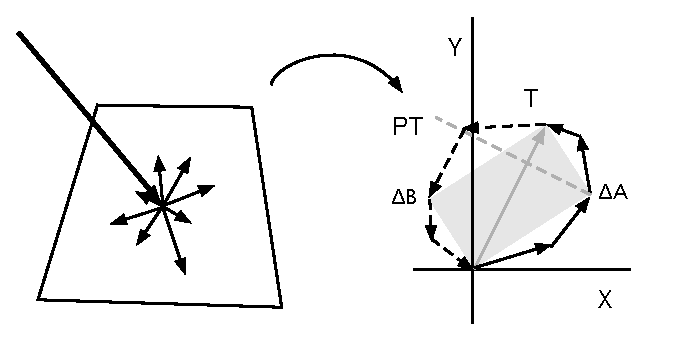
\includegraphics[width=0.6\textwidth]{figures/pt/differential-vectors}
	\caption{每个路径顶点有多个位于同一平面的微分矢量(左),它们构成一个围绕该顶点的多边形线段,这个多边形的面积用来进行该点的足迹}
	\label{f:pt-differential-vectors}
\end{figure}

在式\ref{e:pt-differential-vector}计算微分矢量的公式中,新引入的变量必须要求$\Delta x_j$已知,我们知道对于屏幕空间的两个变量$x,y$,其对应的该两个分量的扰动$\Delta x$和$\Delta y$分别为一个像素大小\footnote{实际上理想情况下,屏幕空间坐标的扰动应该由相邻两条光线的距离决定,由于光线追踪技术并不会仅仅对每个像素发射一条光线,所以一个像素的扰动会导致图像过于模糊,RenderMan中选择使用$1/2$像素尺寸作为扰动大小,这是一个经验值,他们发现小于$1/2$也不会导致图像更加锐化,读者可参考:\url{https://renderman.pixar.com/resources/current/RenderMan/integratorRef.html}了解更多信息。},但是其他变量的扰动应该怎样决定呢?

\cite{a:Pathdifferentialsandapplications}给出了一个简单的启发式(heuristic)用来决定$\Delta x_j$的大小,该启发式基于这样一个观察:即足迹的大小应该反向正比于该点处采样点的密度。例如如果对每个像素均匀发射$N$条光线,则每两条光线之间的距离为$1/\sqrt{N}$,因此采样数量越少,则扰动越大,光线越发散,足迹越大,所以我们也称其为光线发散系数(ray spread)\myindex{光线发散系数}{ray spread factor}。

上式只对于分布式光线追踪算法有用,对于路径追踪算法,每个顶点仅产生一条新的光线,即发散系数为1。\cite{a:Pathdifferentialsandapplications}对路径追踪算法使用另一个启发式,即$1/\sqrt[M]{N}$,这里$M$为路径的深度,所以越长的路径具有更大的扰动。


\cite{a:Pathdifferentialsandapplications}还介绍一种使用每个微分矢量相对于该点整个光照贡献的梯度值来限定$\Delta x_j$的大小,该方法将屏幕空间的过滤函数随光线一起传播,然后以此可以计算微分矢量的梯度变化。

然而,由于路径微分需要对每个顶点做过多微分计算,计算成本比较高,更多的实践方案是以光线微分算法为基础,采取路径微分的发射系数的概念来调整足迹的大小,以满足BRDF分布的影响,这样不需要对每个顶点做太多的积分计算。例如Pixar\footnote{参见:\url{https://renderman.pixar.com/resources/current/RenderMan/integratorRef.html}}就直接根据表面的曲率以及粗糙度来计算发射系数,这样就可以简单地将光线微分扩展至任意表面。







\subsection{协方差追踪}\label{sec:pt-covariance-tracing}
在前面介绍的光线/路径微分技术中,它们通过跟踪中心光线的两条(光线微分)或多条(路径微分)偏移光线的传播来计算这些偏移光线在每个顶点处的微分值,其中的位置微分用于近似一个顶点足迹的大小,进而用于纹理过滤。然而,光线微分仅适用于镜面表面,路径微分虽然能够处理任意表面,但是在每个顶点处都需要大量的微分计算,使得其运用受限,此外,光线微分和路径微分都依赖于屏幕空间的扰动$\Delta x,\Delta y$以及像素的采样数量来计算微分向量,所以它们均不适用于光源路径,忽略光源路径的重要性使得过滤的结果过于模糊。

本节将介绍另一种计算光线足迹的方法,它基于对光照传输进行傅里叶分析,即是分析路径光照传输的频率变化。光照传输的频率域分析是一种比较重要的方法和思路,它主要由\cite{a:AFrequencyAnalysisofLightTransport}开始比较系统的提出,研究光照的局部变化可以用于解决很多光照传输的问题,例如本节讨论的计算路径的足迹,除此之外,光照传输的频率域分析还可以用于下一节讨论的适应性采样和适应性重建,在下一章我们还可以看到光照传输的频率域分析被用于光子映射中的内核尺寸的估计。

本节首先给出一束光线局部光照场的概念,然后给出一种基于方差的光照场的高斯近似,并给出该光照表述在光照传播过程中的各个操作(例如直线传输,阴影遮挡,运动模糊等),最后在光照路径的每一个顶点,该光照表述被用于计算足迹大小。





\subsubsection{光照传输的频率分析}\label{sec:pt-frequency-analysis}
在本章前面第\ref{sec:pt-pixel-filter}节讨论一个像素的值是怎样被计算时,给出了路径追踪算法下屏幕上每个像素颜色值的表达式,它是由一个过滤器以及屏幕空间每个光线采样值的乘积:

\begin{equation}\label{e:pt-pixel-filter}
	L_{\mathcal{I}}={\rm \int}_{\Omega_I\times\mathcal{P}_I}s^{0}_{\mathcal{I}}(\mathbf{x},\omega_{o})L(\mathbf{x},\omega_{o}){\rm d}\omega_{o}{\rm d}\mathbf{x}
\end{equation}

\noindent 为了便于查询和对照原始论文,这里使用了与之相对应的一套标记:$s^{0}_{\mathcal{I}}(\mathbf{x},\omega)$表示像素$\mathcal{I}$处的过滤器,称为一个像素过滤函数(pixel filter function)\myindex{像素过滤函数}{pixel filter function},$\Omega_I\times\mathcal{P}_I$为该像素过滤器的空间-方向(spatial-angular)积分作用域,它由穿过像素$\mathcal{I}$的所有方向以及像素$\mathcal{I}$区域内的所有位置构成。

如果用$\tilde{\rho}(\mathbf{x},\omega_o,\omega)=\rho (\mathbf{x},\omega_o,\omega)\max{((\mathbf{n}\cdot\omega),0)}$表示余弦加权的BRDF分布(cosine-weighted BRDF)\myindex{余弦加权的BRDF }{cosine-weighted BRDF},并代入渲染方程至式\ref{e:pt-pixel-filter}得到:

\begin{equation}
	L_{\mathcal{I}}=L^{0}_{\mathcal{I}}+{\rm \int}\int s^{0}_{\mathcal{I}}(\mathbf{x},\omega_{o})L(\mathbf{y},-\omega)\tilde{\rho}(\mathbf{x},\omega_o,\omega){\rm d}\mathbf{x}{\rm d}\omega_o {\rm d}\omega
\end{equation}

\noindent 这里$L^{0}_{\mathcal{I}}=\langle s^{0}_{\mathcal{I}},L_0\rangle$表示像素$\mathcal{I}$处的自发光。观察上式,我们可以将$s^{0}_{\mathcal{I}}$和余弦加权的BRDF项提前计算出来,该计算结果形成了一个新的间接像素过滤器(indirect pixel filter)\myindex{间接像素过滤器}{indirect pixel filter},以此类推,我们得到一个从摄像机出发$k-$次反弹的间接过滤器:

\begin{equation}\label{e:pt-indirect-filter}
	s^{k}_{\mathcal{I}}(\mathbf{y},\omega)={\rm \int} s^{k-1}_{\mathcal{I}}(\mathbf{x},\omega_o)\tilde{\rho}(\mathbf{x},\omega_o,\omega){\rm d}\omega_o
\end{equation}

\noindent 上式是一个非常有意义的公式,它说明我们可以让一个初始像素过滤器$s^{0}_{\mathcal{I}}$跟随着光线路径一起在场景中传播,路径中每个顶点处的BRDF分布函数会对传播的间接过滤器进行修改,修改后的过滤器将被用于正确的对纹理以及光源进行过滤。

这是一个非常抽象的解释,具体我们怎样利用上式来对纹理或光源进行过滤呢?在传统的路径追踪技术中,反走样依赖于超采样,即对每个像素发射大量的光线,每条光线都需要经历完整的传播过程(即该光线路径上的每个点都需要与场景进行相交计算以决定光线的下一个传播方向)。在该方法中,对于每一条光线,式\ref{e:pt-indirect-filter}中的$s^{k}_{\mathcal{I}}$只是一个普通的权重标量值,它唯一决定了对每个顶点处纹理的一个采样位置,光线追踪算法要保证足够的光线数量才能使得对纹理的采样不会出现走样。

纹理过滤的思路是使用少量的光线,并将像素的采样率传播到每个顶点处进而对纹理进行过滤。然而单个光线并不知道与之相邻的光线的存在,因此光线/路径微分技术使用一些虚拟的偏移光线来协助中心光线传播像素的采样率。这里同样需要使用类似的思路,设想式\ref{e:pt-indirect-filter}仍然是针对一条光线,然而除了中心光线以外,我们还发射了一些额外的偏移光线,这时$s^{k}_{\mathcal{I}}$就不再是一个单一的标量值,而是一个真正的过滤器,如果我们能够正确地传播$s^{k}_{\mathcal{I}}$,则可以正确地对纹理进行过滤。

与光线/路径微分技术不同的是,这里不再通过计算光线微分的方式来计算足迹。\cite{a:AFrequencyAnalysisofLightTransport}首先提出将一个过滤器看做一个局部光照场(local light field)\myindex{局部光照场}{local light field},因此这里的局部光照场并不是一个关于光照的分布,而是一个用来表述一束光局部特征的空间-方向分布函数(spatial-angular distribution)\myindex{个空间-方向分布}{spatial-angular distribution},它表征了一束光的分散和分布情况,例如空间分布范围越大,其过滤范围越大;方向分布越分散,则其传播过程空间分布越容易发散,这和前面光线/路径微分计算出来的光线足迹类似。因此,如果我们能够正确计算这个局部光照场随着光线的传播,就能够对每个顶点的纹理进行正确过滤。

我们用$\ell(\mathbf{z})$表示局部光照场,局部光照场是一个4D\footnote{我们将在后面看到,当局部光照场用于运动模糊等与时间相关的运用时,局部光照场还可以表示为一个5D矢量,新增的一个分量为时间。}矢量,其中$(x,y )$表示空间分量,$(\theta,\phi)$表示方向分量,如图\ref{f:pt-local-light-field}右边小图所示,一个局部光照场可以用下式表示:

\begin{equation}
	\ell(\mathbf{z})=(x,y,\theta,\phi)
\end{equation}

\noindent 局部光照场的示意图如图\ref{f:pt-local-light-field}所示,在该图中只有一条称为中心光线(central ray)\myindex{中心光线}{central ray}的真实光线,其他都是虚拟的偏移光线,这些光线各自具有不同的位置和方向,它们构成一个局部光照场,局部光照场的所有光线都位于同一平面,该平面垂直于中心光线(即光线传播方向)。

\begin{figure}
	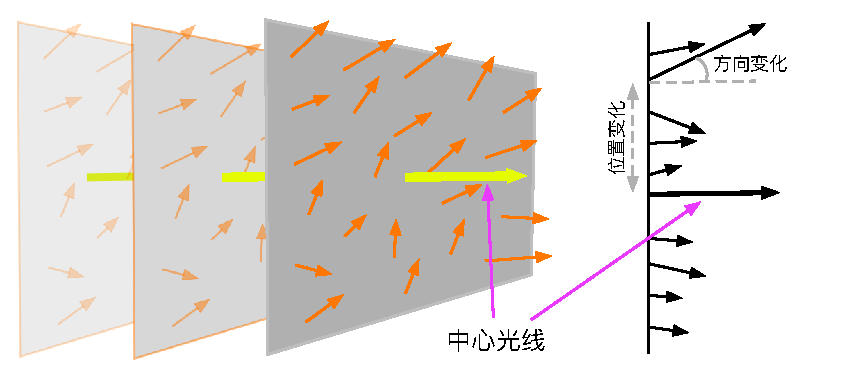
\includegraphics[width=\textwidth]{figures/pt/local-light-field}
	\caption{局部光照场是一个空间-方向分布函数,该分布函数的范围就代表了每个顶点处的足迹,只要找到某种方法能够让局部光照场随着中心光线一起传播,就能够正确地对每个顶点的纹理进行过滤}
	\label{f:pt-local-light-field}
\end{figure}

对于中心光线在每个特定位置(例如路径的每个顶点)处的局部光照场,我们感兴趣的是该局部光照场的面积扩展(extent)形状,所以不需要记录每个虚拟光线的真实位置。因此在参数表述上,局部光照场的空间分布是在正切面上相对于中心光线的距离,而方向是相对于中心光线的方向,如图\ref{f:pt-local-light-field}右边小图所示。此外,在后续的操作数推导计算中,有时还用$\tan \theta\approx\theta$来近似由方向变化导致的空间变化。

因此式\ref{e:pt-pixel-filter}中的$s^{0}_{\mathcal{I}}$并不像前面讨论的传统路径追踪算法中的权重函数一样,那里的$h(p)$仅是一个2D的空间分布函数,它对屏幕空间每个位置的光照值给予一个权重值,这里的像素过滤器$s^{0}_{\mathcal{I}}$还需要包含一个方向,对于初始的$s^{0}_{\mathcal{I}}$的值,它就是$h(p)$中的各个位置,加上从摄录像出发经过这些位置的方向。

那里怎么计算光照场的传播过程呢?\cite{a:AFrequencyAnalysisofLightTransport}通过将光照场变换到傅里叶空间,然后将传输过程中的直线传播,遮挡计算,光线与表面的BRDF交互等过程转变成一些线性变换函数,这些函数与傅里叶空间的光照场进行对应的卷积或者内积等计算。在Durand的原始论文中,他们使用一个能够包含局部光照场的一个盒子形状来表示局部光照场,如图\ref{f:pt-local-light-field-representation}左二图所示,这个盒子可以使用一个频宽矢量(bandwidth vector)$[B_x,B_u]$表述,然后这个矢量在光线传输中被执行上述线性变换,从而计算局部光照场的传输,其他一些方法如\cite{a:FrequencyAnalysisandShearedReconstructionforRenderingMotionBlur}则使用一个切变形状表述,如图\ref{f:pt-local-light-field-representation}右二图所示。这些表述虽然比较高效,但是这些形状不能完全反应局部光照场的面积扩展情况,我们在本节将要讨论的是另一种更加精确的计算方法,它用一个椭圆形形状来近似局部光照场的扩展形状,如图\ref{f:pt-local-light-field-representation}右边小图所示,这个椭圆形高斯分布可以使用局部光照场的协方差矩阵来表示,所以对该形状的一些传输操作转变为各种矩阵变换,因此计算精度更高,同时也相对比较高效。


\begin{figure}
\begin{fullwidth}
	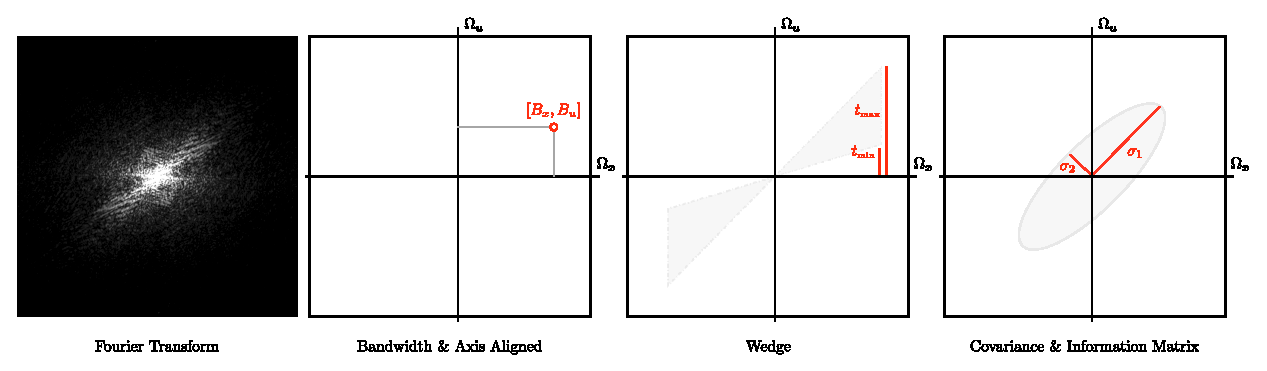
\includegraphics[width=\thewidth]{figures/pt/local-light-representation}
	\caption{几种常见局部光照场的函数表述,局部光照场主要关注光线的局部变化,即是在正切面上的扩展形状,这些方法使用不同的函数和参数来近似光照场局部变化的形状(图片来自Belcour)}
	\label{f:pt-local-light-field-representation}
\end{fullwidth}
\end{figure}


由光照场的定义也可以看出,光照场仅表示一个空间-方向分布函数,它与真正的光照值是无关的,因此任意的空间-方向分布都可以表示该分布代表的几何区域的尺寸,因此光照场相关的技术也可以用于传播双向路径追踪技术中的光源路径,因为光源分布也可以表示为一个空间方向分布,我们会在后面详细讨论相应的内容。





\subsubsection{协方差矩阵}
\cite{a:FundamentalsofTextureMappingandImageWarping}指出,当屏幕空间圆形的过滤区域在场景中随着光线一起传播并投影到纹理空间后,如图\ref{f:pt-elliptical-filter}左下角小图所示,它会更接近于一个椭圆形区域,如图\ref{f:pt-elliptical-filter}右上角小图所示。为了满足这种过滤器形状在传播中变换的需求,Heckbert提出使用一个空间分布的协方差矩阵(covariance matrix)\myindex{协方差矩阵}{covariance matrix}\footnote{实际上原论文只要求一个对称矩阵,该对称矩阵用于将圆形形状的高斯过滤器转换为椭圆形的高斯过滤器,显然协方差矩阵满足这个要求。}来表述的椭圆形高斯过滤器(elliptical Gaussian filter)\myindex{椭圆形高斯过滤器}{elliptical Gaussian filter},\cite{a:5DCovarianceTracingforEfficientDefocusandMotionBlur}在此基础上提出一种使用协方差表述的更简单的近似模型。

\begin{figure}
	\sidecaption
	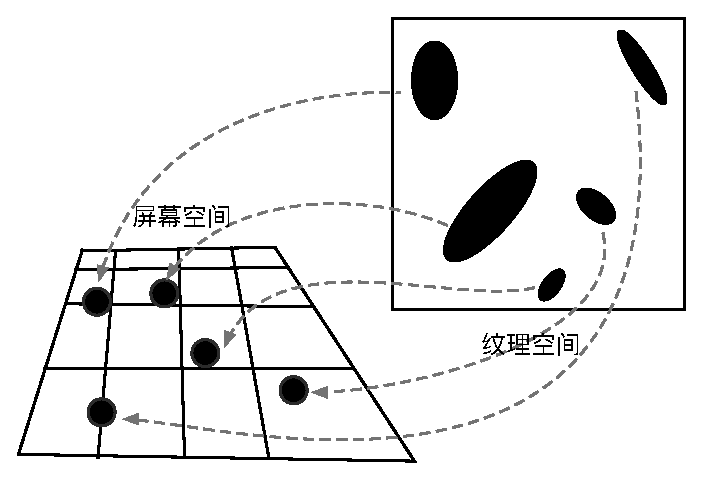
\includegraphics[width=0.6\textwidth]{figures/pt/elliptical-filter}
	\caption{屏幕空间的圆形的过滤器在经过光线路径传播之后,会以接近椭圆形的形状投影在纹理空间,因此在光照传播过程中需要使用一种支持椭圆形形状的过滤器,椭圆形高斯过滤器就是其中一种比较理想的选择,它基于一个对称矩阵来构造,而协方差矩阵就是一个很好的选择}
	\label{f:pt-elliptical-filter}
\end{figure}

这里的协方差是指局部光照场$\ell(\mathbf{z})$的傅里叶变换$\hat{\ell}(\mathbf{z})$的协方差,因为我们需要研究的是局部光照场的局部方差和各向异性,它需要通过该光照场的频率域的振幅来分析。我们用$\sum$来表示该协方差矩阵,局部光照场傅里叶变换振幅谱(amplitude spectrum)\myindex{振幅谱}{amplitude spectrum}的协方差矩阵的每一项为:

\begin{equation}
	\sum\nolimits_{i,j}\equiv{\rm \int\limits}_{\mathbf{z}\in\Omega}\langle\mathbf{z},\mathbf{e}_i\rangle\langle\mathbf{z},\mathbf{e}_j\rangle |\hat{\ell}(\mathbf{z})|{\rm d}\mathbf{z}
\end{equation}

\noindent 这里$\Omega=\Omega_x\times\Omega_y\times\Omega_\theta\times\Omega_\phi$表示一个4D的傅里叶空间,$|\hat{\ell}(\mathbf{z})|$表示该局部光照场的振幅。有了协方差矩阵,\cite{a:5DCovarianceTracingforEfficientDefocusandMotionBlur}提出的近似椭圆形高斯过滤器为:

\begin{equation}
	g(\mathbf{z})=\mathrm{e}^{-\mathbf{z}^{T}\sum^{-1}_g \mathbf{z}}
\end{equation}

\noindent 这里$\mathbf{z}^{T}\sum^{-1}_g \mathbf{z}$表示的是对变量$\mathbf{z}$执行线性变换的过程,所以对该椭圆高斯过滤器的所有变换操作都可以作用到这个协方差矩阵上去,反之,在光照传播过程中,我们只需要将所有交互变换作用到这个协方差矩阵上,就可以计算整个光照场的传播过程,所以这就是该方法称之为协方差追踪(covariance tracing)\myindex{协方差追踪}{covariance tracing}的原因,所以剩下的事情就是将这些传播过程中的操作正确作用到光照场的协方差矩阵上。





\subsubsection{光照传播操作数}
在光照传播过程中,初始光照场随着光线一起传播,由于光照场是一个关于空间-方向的分布,所以传播过程中的这些操作都可以转化为对方向和空间位置的某种线性变换操作,它们各自分别可以用一个线性变换矩阵表述。如果我们把光照场传播过程中的每种原子操作定义为一个独立的操作数,这些操作数串联起来就构成了光照场随着光线路径的整个传播公式。例如以下是一条$LSDE$路径的传输操作:

\begin{equation}
	LSDE\to\mathbf{L}_(d_1,d_2)\circ\mathbf{T}_{d1}\circ\mathbf{R}_{\rho d}\circ\mathbf{T}_{d2}\circ\mathbf{O}\circ\mathbf{T}_{d3}\circ\mathbf{R}_{\rho_s}\circ\mathbf{T}_{d4}(\hat{\ell})
\end{equation}

\noindent 这里$LSDE$表示一条光线路径,$\mathbf{L}_(d_1,d_2), \mathbf{T}_d, \mathbf{R}_\rho$以及$\mathbf{O}$称为一些原子操作数,它们将一个光照场映射为另一个光照场,这些操作数各自分别对应于光线传播过程中的一个物理过程,例如直线传输,可见性剔除,反射,运动模糊(注意,本节讨论的光照场是一个包含时间维度的5D分布)等。以下简要描述每个传输操作数:

\begin{itemize}
	\item \textbf{直线传输 } 直线传输操作定义辐射亮度$\mathbf{L}$沿中心光线方向直线传输空间距离为$d$的距离直线传输操作记为$T_d$。
	\item \textbf{阴影遮挡 } 阴影遮挡定义当中心光线没有被任何物体遮挡,而局部光照场接近某个物体时可能产生的部分阴影遮挡,阴影遮挡操作记为$\mathbf{O}$。
	\item \textbf{再参数化 } 如前所述,局部光照场的参数化是围绕中心光线来表述的,当中心光线与表面相交时,如下面即将讨论的反射操作都是围绕表面法线来表述的,所以我们需要将局部光照场参数表述变换到表面的正切面,这称为再参数化(reparametrization)\myindex{再参数化}{reparametrization},记为$\mathbf{Rot}_\alpha$和$\mathbf{P}_\alpha$。局部光照场的再参数化也使得后面的运动处理变得简单,因为当带有时间维度的局部光照场表述被再参数化到物体本地空间时,后续的所有操作可以忽略时间维度,使之变为一个静态的4D变换,因为运动都是相对的。
	\item \textbf{曲面再参数化 } 当表面为曲面时,局部光照场中的光线可能并不位于中心光线所在交点的正切面上,此时我们需要考虑曲面曲率对局部光照场传输的影响,称操作称为曲面再参数化(curvature reparametrization)\myindex{曲面再参数化}{curvature reparametrization},记为$\mathbf{C}_K$,此时通常曲面的曲率会被记录到变换矩阵中。
	\item \textbf{反射,折射 } 反射和折射操作定义局部光照场在物体表面基于BRDF或BTDF反射分布$\rho$的反射或折射的过程,记为$\mathbf{R}_\rho$和$\mathbf{Tr}_\rho$。
	\item \textbf{聚焦 } 聚焦定义局部光照场通过一个薄的透镜的过程,该操作有两种定义:一种在传感器上输出辐射照度,另一种输出辐射亮度(这样使得多个透镜可以被叠加使用),聚焦操作定义为$\mathbf{L}(d1,d2)$。
	\item \textbf{参与媒介 } 当局部光照场通过参与媒介时,该过程被两种操作表述:即衰减操作$\mathbf{A}$和散射操作$\mathbf{S}\rho$($\rho$为分段函数)。
	\item \textbf{运动 } 运动的物体对局部光照场增加了一个时间维度,使之成为一个5D分布函数。为了跟踪时间变化,通常将带有时间维度的局部光照场再参数化到运动物体的局部静态空间,因为运动都是相对的,这使得所有其他操作可以在4D空间进行,最后再将局部光照场的表述再参数化到全局包含时间维度的空间,这大大简化了时间维度的处理,使得局部频率分析可以处理如运动模糊等效果。运动操作记为$\mathbf{M}_{v,r}$。
\end{itemize}

\cite{a:AFrequencyAnalysisofLightTransportfromtheorytoimplementation}通过对上述的各个过程进行分析推导出了每个操作的矩阵表示,请读者参阅原始论文获取更详细的推导信息和形式,为了对这些操作建立直观的概念,我们这里仅分析直线传输操作。

\begin{figure}
\sidecaption
	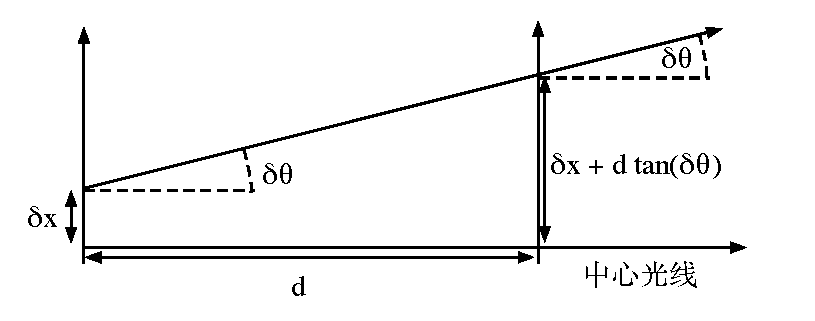
\includegraphics[width=0.65\textwidth]{figures/pt/travel}
	\caption{给定局部光照场的参数化表述$(\delta x,\delta\theta)$,经过距离为$d$的直线传输后,通过坐标变换可以建立起直线传输的操作矩阵,它是一个切变变换}
	\label{f:pt-travel}
\end{figure}

为了简化描述,这里用一个2D分布进行说明,即局部光照场仅包含一个方向$\delta\theta$和一个空间位置$\delta x$,如图\ref{f:pt-travel}所示。当局部光照场经过距离$d$的直线传输后,新的局部光照场可以表述为以下线性变换:

\begin{equation}
	\begin{aligned}
		\mathbf{T}_d(\ell)(\delta x,\delta\theta)&=\ell(\delta x-d\tan{(\delta\theta)},\delta\theta)\\
		&\approx\ell(\delta x-d\delta\theta,\delta\theta)
	\end{aligned}
\end{equation}

\noindent 上述第二行的近似使用了前面描述的一阶近似,这是基于局部光照场方向变化无限小的假设。上述的变换实际上是一个切变变换(shear transform)\myindex{切变变换}{shear transform},直线传播使得局部光照场的空间分布发生变化,而方向分布不变,如图\ref{f:pt-travel}所示。上式表述的切变变换可以由以下线性变换矩阵表述:

\begin{equation}
	A=\begin{pmatrix}
		1 & 0 & -d & 0 & 0 \\
		0 & 1 & 0 & -d & 0 \\
		0 & 0 & 1 & 0 & 0 \\
		0 & 0 & 0 & 1 & 0 \\
		0 & 0 & 0 & 0 & 1 \\
	\end{pmatrix}
\end{equation}

我们不会在这里推导所有这些原子操作变换矩阵的过程,\cite{a:AFrequencyAnalysisofLightTransportfromtheorytoimplementation}包含了所有上述这些变换矩阵的推导和最终形式。但是这里需要注意的是,这些操作变换矩阵的推导有些是使用数值方法近似的,例如阴影遮挡是使用体素结构表述空间物体的法线分布,然后使用光线步进(ray marching)的方式近似计算,所以这些操作变换矩阵的精度和计算效率也是局部频率分析方法以后研究的方向。一旦获得这些原子操作矩阵,局部光照场在传输过程中每个物理过程的计算则变成非常简单的矩阵运算,这比光线/路径微分技术中的微分计算要高效得多(因为矩阵计算比微积分计算要高效)。图\ref{f:pt-operators}是一个简单的局部光照场传输的示例,该示例中包含了直线传输,表面反射等物理操作过程。

\begin{figure}
	\sidecaption
	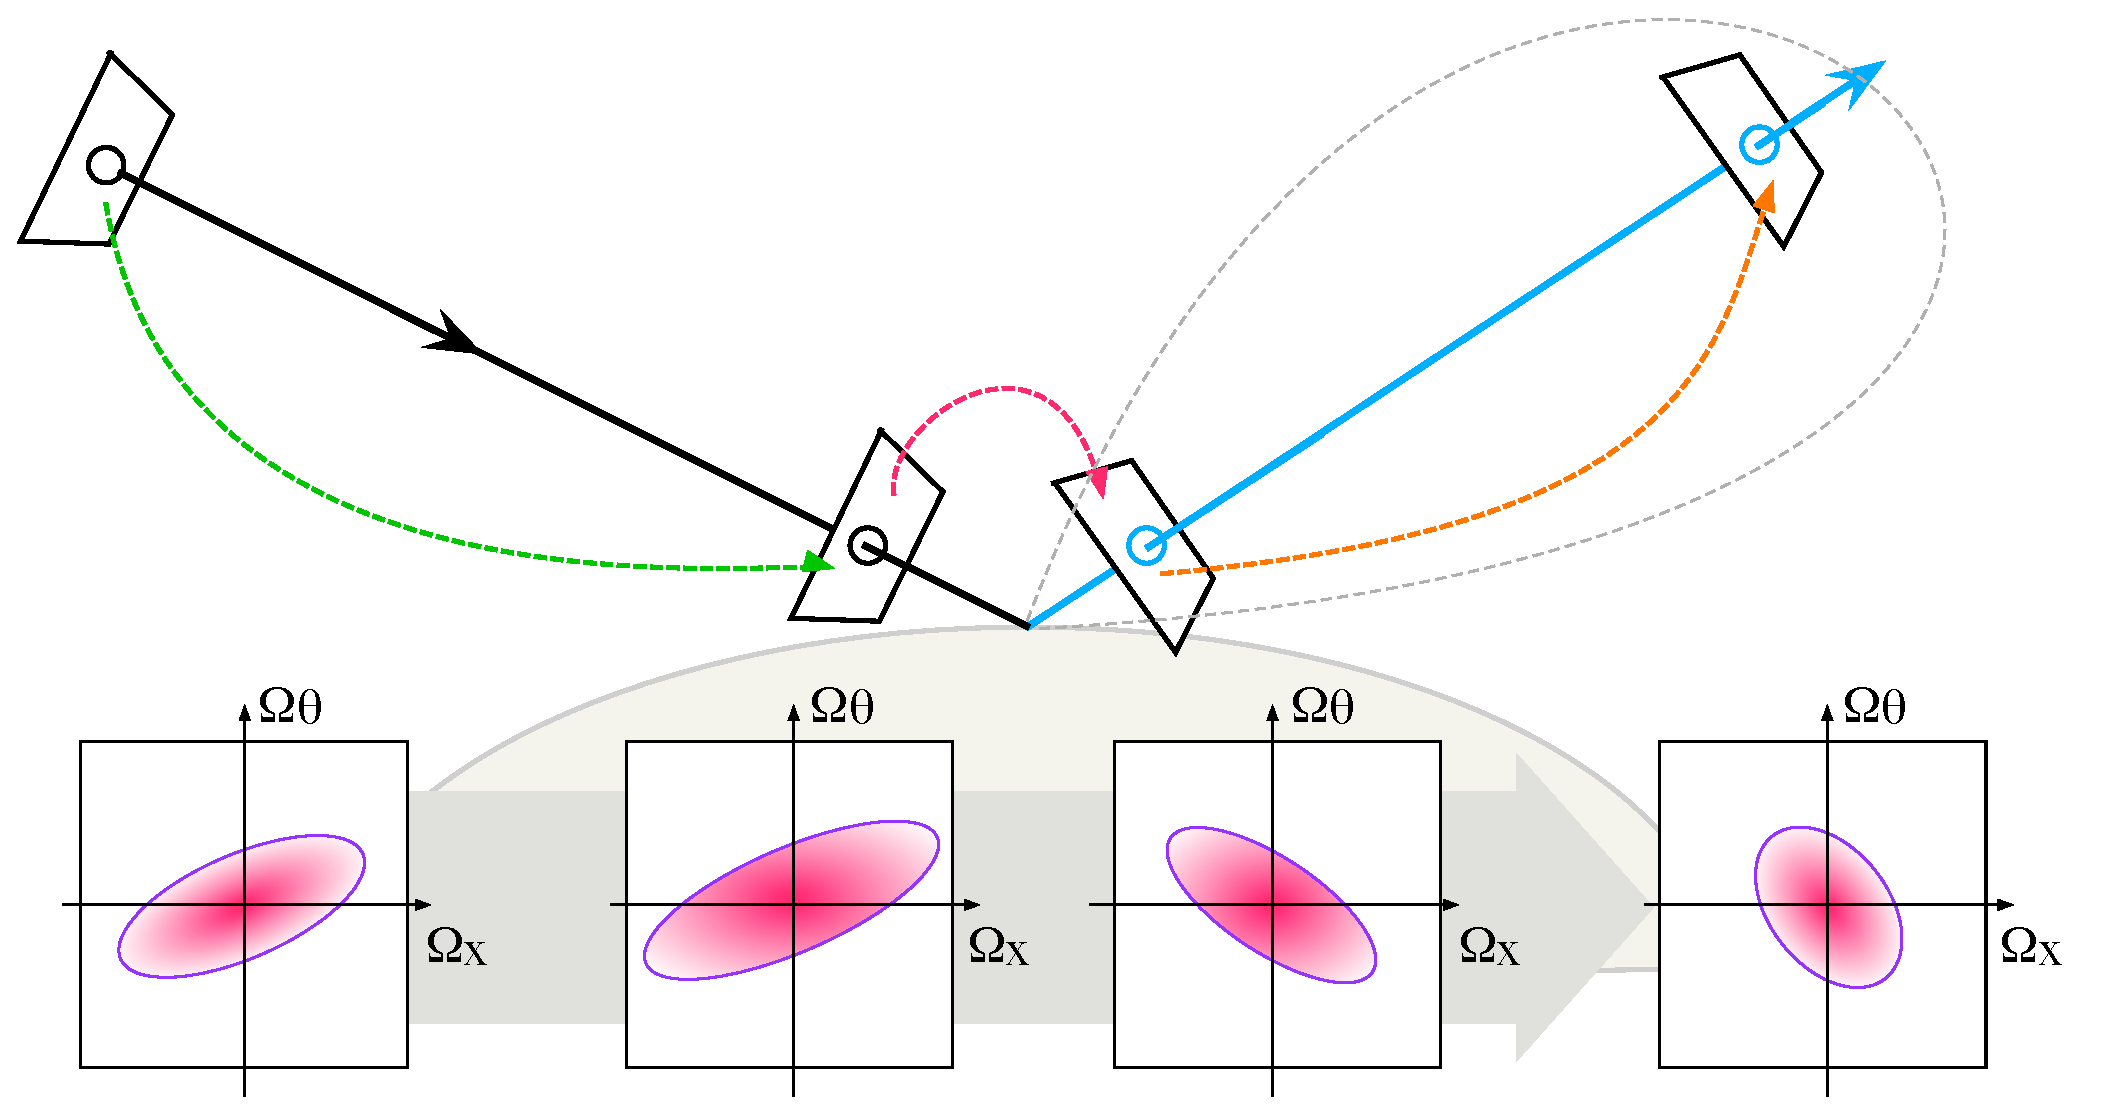
\includegraphics[width=0.65\textwidth]{figures/pt/operators}
	\caption{光照传输过程中的每一个物理过程,都可以转化为对局部光照场空间和方向上的某种变换操作,这些原子操作都可以使用一些变换矩阵来近似,这样边可以简单地跟踪局部光照场的传播过程。注意,这里为了便于演示只画出了2个维度:一个空间维度$\Omega_x$和一个方向维度$\Omega_\theta$}
	\label{f:pt-operators}
\end{figure}





\subsubsection{协方差追踪在路径追踪技术中的运用}
给定上述局部光照场的协方差追踪公式,以及局部光照场在传播过程中的各种物理操作数的矩阵形式,本节我们将讨论这些基础工作怎样被集成于传统的路径追踪算法中去,这涉及以下重要问题:

\begin{enumerate}
	\item 怎样定义摄像机路径和光源路径的初始局部光照场?
	\item 在每个顶点处怎样获取纹理采样所需的过滤函数?
	\item 光源路径和摄像机路径的协方差矩阵怎样合并?
	\item 协方差最终如何集成到传统以光线微分技术为基础的渲染器中?例如RenderMan和PBRT。
\end{enumerate}

本节我们将按照这些问题的顺序逐步分析协方差追踪在路径追踪技术中的运用。

前面我们已经讨论过摄像机路径的起始局部光照场,它就是每个像素$\mathcal{I}$处的过滤器$s^{0}_{\mathcal{I}}(\mathbf{x},\omega)$,跟一般的过滤器(只是空间位置的函数$h(p)$)不同的是,局部光照场是一个空间-方向分布,所以我们要需要记录每条偏移光线的方向。

设想双向路径追踪中路径的总长度为$n$,其中摄像机路径长度为$k$,以下我们用顶点表示方法,设我们已经求出$k$点处的摄像机方向的局部光照场$s^{k}_{\mathcal{I}}(\mathbf{x}_{k-1},\mathbf{x}_k)$,假定$k$点处来自光源路径($k+1$点)的辐射亮度为$L^{n-k}(\mathbf{x}_{k},\mathbf{x}_{k+1})$,则该路径的总的辐射亮度贡献为:

\begin{equation}
	L^{n}_\mathcal{I}={\rm \int} s^{k}_{\mathcal{I}}(\mathbf{x}_{k-1},\mathbf{x}_k)\rho (\mathbf{x}_k)L^{n-k}(\mathbf{x}_{k},\mathbf{x}_{k+1}){\rm d}\mathbf{x}_{k-1}{\rm d}\mathbf{x}_{k}{\rm d}\mathbf{x}_{k+1}
\end{equation}

\noindent 由于光源路径是通过某个光源上的一个采样点的辐射亮度$L^{0}$通过与各个顶点的余弦加权的BRDF相乘得来的,因此和前面求摄像机路径局部光照场的思路类似,我们可以表示$k+1$点的辐射亮度为:

\begin{equation}\label{e:pt-light-filter}
\begin{aligned}
	L^{n-k}(\mathbf{x}_{k},\mathbf{x}_{k+1})={\rm \int} \tilde{\rho}(\mathbf{x}_{k+2},\mathbf{x}_{k+1})  L^{n-k-1}(\mathbf{x}_{k+1},\mathbf{x}_{k+2}){\rm d}\mathbf{x}_{k+2}
\end{aligned}
\end{equation}

\noindent 而最终光源路径的起始辐射亮度为某个光源上的一个采样点$L^{0}(\mathbf{x_n})$,同摄像机光线一样,这仍然是单个采样值,为了构建一个局部光照场,我们需要从$L^{0}(\mathbf{x_n})$附近选取多个虚拟的采样点用于构建局部光照场,这个局部光照场的空间-方向分布对应于光源本身的分布。

将式\ref{e:pt-pixel-filter}和式\ref{e:pt-light-filter}直接合并是不合适的,光源路径的局部光照场和摄像机路径的局部光照场的频率可能是不一样的,这就会导致合并的结果更模糊。\cite{a:AntialiasingComplexGlobalIlluminationEffectsinPath-space}使用了取两个路径的局部光照场的卷积的形式来计算合并后的局部光照场,即:

\begin{equation}
	\sum\nolimits_{\mathbf{x}_k}=\sum (\hat{s}^{k}_{\mathcal{I}}\star_k \hat{L}^{n-k})=\sum(\hat{s}^{k}_{\mathcal{I}})\oplus_k\sum(\hat{L}^{n-k})
\end{equation}

\noindent 这里$\hat{s}^{k}_{\mathcal{I}}$和$\hat{L}^{n-k}$分别表示摄像机路径和光源路径传播过来的$4\times 4$的协方差矩阵,$\oplus_k$表示一个受限的矩阵求和,它只将两个矩阵中心相交的$2\times 2$矩阵进行相加。

现在来梳理一下整个协方差追踪的过程,为了简化描述并突出重点步骤,这里只针对传统的单项路径追踪,这个过程(针对单个光线路径光照的计算)简述如下:

\begin{enumerate}
	\item 首先构造一条摄像机起始光线,它是以摄像机为起点,穿过屏幕区域某个位置$\mathcal{I}$的一条光线。
	\item 以该光线为中心光线,同样以摄像机为起点发射几条偏移光线,这些偏移光线在屏幕区域的位置$(x,y)$和方向$(\theta,\phi)$构成一个4D的局部光照场$s^{0}_{\mathcal{I}}$,并求出该局部光照场的协方差矩阵。
	\item 沿着光线与场景的第一个交点$\mathbf{x}_1$的方向按照相关的局部光照场传播操作数传播协方差矩阵。
	\item 当协方差矩阵被传播至$\mathbf{x}_1$时,此时进入算法的重点,即对纹理进行采样,这是我们需要根据$\mathbf{x}_1$处的协方差矩阵求出一个过滤函数$h(p)$用于对纹理进行过滤。这个对纹理采样的结果就是得出该顶点的BRDF分布函数$\rho(\mathbf{x}_1,\omega_o,\omega)$。
	\item 根据$\mathbf{x}_1$处的BRDF分布函数对反射或折射方向进行采样,这个过程即计算出$\tilde{\rho}(\mathbf{x}_1,\omega_o,\omega)$。
	\item 将计算出的$\tilde{\rho}(\mathbf{x}_1,\omega_o,\omega)$代入式\ref{e:pt-pixel-filter}计算出反射/折射后的协方差矩阵,然后重复上述过程直到该条路径追踪结束。
\end{enumerate}

由于协方差矩阵反应了局部光照场的扩展大小,即是该点的足迹的大小,因此可以通过该点的协方差矩阵求出该点的一个过滤函数$h(p)$。\cite{a:AntialiasingComplexGlobalIlluminationEffectsinPath-space}中给出了一个求过滤函数的公式:

\begin{equation}
	h(\mathbf{u},\omega)=g([\mathbf{u},\omega]^{T}\sum^{k}[\mathbf{u},\omega])/K_g
\end{equation}

\noindent 这里$g(x)$是任意一个1D的过滤函数,$K_g=(2\pi)^2 \sqrt{|\sum|}$,它表示一个用于归一化的最大边界。

上述方法适合于直接针对高精度的纹理进行过滤,它直接将一个过滤函数作用于纹理采样函数上。然而很多时候,纹理是使用多级纹理等技术预过滤的,此时我们需要像光线/路径微分技术那样给出一个足迹大小来让纹理采样函数选择正确的多级纹理的层级,这种情况下我们需要直接根据该点的协方差矩阵求出该点的足迹大小,这样的用法也使得协方差追踪可以用于传统以光线微分为基础的路径追踪渲染器中。

在光线微分算法中,一个顶点处的光线微分是通过该点处光线$(\mathbf{P},\mathbf{D})$相对于屏幕空间坐标$(x,y)$的偏导数来求的,即:$({\rm \partial}\mathbf{P}/{\rm \partial} x,{\rm \partial}\mathbf{P}/{\rm \partial} y)$和$({\rm \partial}\mathbf{D}/{\rm \partial} x,{\rm \partial}\mathbf{D}/{\rm \partial} y)$。由于一个协方差矩阵包含了该点处的局部光照场,即是该点某个空间-方向分布函数,所以我们可以从这个$4\times 4$协方差矩阵提取出计算光线微分需要的这些偏导数。

假设局部光照场表示为高斯过滤器,有前面的定义可知,我们需要首先求出协方差矩阵的逆矩阵$C=\sum^{-1}$,对$C$的第一个$2\times 2$块组成的矩阵进行特征分解可以用于计算空间偏导数:

\begin{equation}
	\begin{aligned}
		 \cfrac{{\rm \partial}\mathbf{P}}{{\rm \partial} x}=& \cfrac{\sqrt{{\Lambda_{\mathbf{x}_0} }}}{2\pi}\mathbf{x}_0 \\
		 \cfrac{{\rm \partial}\mathbf{P}}{{\rm \partial} y}=& \cfrac{\sqrt{{\Lambda_{\mathbf{y}_1}}}}{2\pi}\mathbf{x}_1 \\
	\end{aligned}
\end{equation}

\noindent 其中,$\{\mathbf{x}_0,\mathbf{x}_1\}$为空间特征向量,$\{\Lambda_{\mathbf{x}_0},\Lambda_{\mathbf{x}_1}\}$空间特征值,由于每个特征值表示的是方差而不是标准差,所以需要开平方。同理通过$C$的最后一个$2\times 2$块构成的矩阵可以求出方向偏导数为:

\begin{equation}
	\begin{aligned}
		 \cfrac{{\rm \partial}\mathbf{D}}{{\rm \partial} x}=& \cfrac{\sqrt{{\Lambda_{\omega_0}}}}{2\pi}\omega_0 \\
		 \cfrac{{\rm \partial}\mathbf{D}}{{\rm \partial} x}=& \cfrac{\sqrt{{\Lambda_{\omega_1}}}}{2\pi}\omega_1 \\
	\end{aligned}
\end{equation}

\noindent 因此,协方差追踪可以很容易地集成到现有的以光线微分为基础的渲染器中,例如PBRT,Mitsuba等,\cite{a:Covariancetracingsourcecode}提供了关于协方差追踪的相关源代码。

本节讨论了协方差追踪在纹理过滤中的运用,在下一节还会进一步将协方差追踪运用于适应性采样和过滤中用于实现路径追踪算法中的降噪处理。协方差追踪算法通过使用一个椭圆形高斯过滤器来近似一个局部空间-方向分布函数,并进一步使用该空间-方向分布函数的协方差矩阵来近似这个过滤函数,使得局部光照场的频率域分析变得简单而高效。然而这也正是协方差追踪算法的缺点,即它仅用一个椭圆形过滤器来近似光照场的局部特征,实际光照场可能还会有更复杂的形状分布,对局部光照场更高精度的局部特征表述也是该领域今后研究的重要方向。







\section{降噪技术}\label{sec:pt-denoising}
上一节我们讨论了路径追踪算法中在路径的每个顶点处由于对纹理的采样不足导致的纹理走样(texture aliasing)\myindex{纹理走样}{texture aliasing},以及怎样通过跟踪光线的足迹大小来提供一个过滤范围参考值,从而有效地对纹理进行过滤以消除纹理走样。

不同于一般的信号采样,它们通常使用一个固定的采样率,因此走样\myindex{走样}{aliasing}来源于由于采样率不能覆盖原始信号的频率带宽(这相当于使用一个均匀分布采样的蒙特卡洛方法),通常蒙特卡洛方法使用的采样并不是均匀分布的,这些随机数的统计特征还引入了方差,而方差导致了图像中的噪点,因此在路径追踪技术中除了需要处理由于采样不足导致的走样(这通过过滤来实现),还需要减少由于随机变量方差导致的噪点。虽然一些方法通过改善路径采样方法(如重要性采样,双向路径追踪,梅特波利斯光照传输等)来控制方差,本节将要介绍的却是一种与采样技术无关的控制方差的方法,我们称这些特定的与采样方法无关的控制方差的方法为降噪技术\footnote{降噪技术本意通常仅指针对图像的局部误差特征分布进行适应性的图像重建,但正如本节即将看到的,适应性采样和适应性重建图像是组合使用的,所以本节讨论的降噪技术同时包含适应性采样和适应性重建。}(denoising)\myindex{降噪技术}{denoising}。

本节讨论的降噪技术涉及适应性采样和适应性重建两个概念。由于图像的方差分布通常是随着图像的局部特征而变化的,因此适应性采样(adaptive sampling)\myindex{适应性采样}{adaptive sampling}就是根据前序步骤计算的图像的局部特征来适应性的调整后续采样的密度分布,以满足图像的方差特征,因此它是一个迭代的过程,它由前面的采样结果来决定后续采样的密度分布,这种采样方法区分于一般的对整个图像使用预先设定的固定的概率密度函数的采样方法。

适应性重建(adaptive reconstruction)\myindex{适应性重建}{adaptive reconstruction}通过分析图像的局部特征来构造不同的重建过滤器,也称为适应性过滤(adaptive filtering)\myindex{适应性过滤}{adaptive filtering}。由于图像的局部特征差异,对整个图像使用相同的过滤器会使得高频部分过于模糊,它们应该使用更小范围的过滤器来避免这种模糊,因此适应性重建通过共享像素之间的信息来减少方差。适应性采样和适应性重建通常是同时存在的,例如适应性采样的结果通常需要进行适应性重建,但是有时适应性重建也可以根据其他信息来进行过滤范围选择。

根据适应性采样的策略不一样,我们将降噪技术分为两大类:第一种方法通过直接对光照传输过程进行分析来指导适应性采样,它们不需要通过考虑其他样本值来提供适应性采样信息,因此称为先验方法(a priori methods)\myindex{先验方法}{a priori methods}\footnote{在英语中,"a priori"表示用已知真实的事实或原则去推断可能出现的结果,即由因及果,这里表示我们从光照传输过程(即路径采样算法)本身着手分析图像的特征分布;而后面的"a posteriori"则与之相反,它是从已知事实推断可能导致该事实的原因,即由果及因,所以后验方法表示从光照传输的结果(即图像)着手分析导致该图像(结果)的光照传输特征。},先验方法可以通过微分几何的方法来分析光线传输的局部特征,也可以通过频率域分析的方式来分析和表述光照传输的局部特征,本节我们将重点讨论后者,但是它们两者的基本思路是一致的,先验方法由于直接对光照传输进行分析,因此可以从更高维度分析走样,从而可以比较容易地处理运动模糊(时间维度),聚焦(方向维度)等效果;与之相反,后验方法(a posteriori methods)\myindex{后验方法}{a posteriori methods}则需要通过分析一些样本值的结果来获取适应性采样信息,这样的方法通常只能是基于图像空间(image space)的方法,因此通常具有更高的计算效率,这也是当前工业中(如Disney,Pixar和维塔数码等)比较流行的降噪技术,参见\cite{a:RecentAdvancesinAdaptiveSamplingandReconstructionforMonteCarloRendering}。








\subsection{先验方法}
在路径采样的过程中,我们无法预测一个场景图像的分布特征,因为它是路径采样的结果,因此适应性采样试图将采样的过程分离为多个迭代的过程,即首先生成少量稀疏的采样路径,并用这些采样的结果来分析图像的局部特征,然后它被用来计算出一个具有指导性的采样密度分布,这个指导采样分布被用于后续的采样过程,因此适应性采样是一个迭代的过程,随着迭代的推进,采样密度的预测越来越接近真实图像的分布,从而能够根据图像的特征进行适应性采样:在频率变化较高的区域放置更多的采样数量,而在低频部分放置更稀疏的采样数量。

适应性采样的关键在于怎样根据前序采样过程或结果生成后序采样过程的指导(或建议)采样密度分布,在渲染中这主要有两类方法:第一类方法通过分析光照传输的过程来辨识图像的局部特征,而第二类方法通过分析采样的结果(即图像)来分析图像的局部特征,前者是由因及果的方法,因此称为先验方法(a priori methods)\myindex{先验方法}{a priori methods},它也是本节要讨论的方法,而我们将在下一节讨论第二类后验方法。

路径采样中的每条路径彼此都是独立的,因此传统的路径追踪算法无法从其采样过程获得任何图像分布局部特征的信息,要想获得这样的信息除了跟踪每条光线的传输,还得跟踪和分析其传输过程中局部(相邻光线)的变化。当然我们不应该采用同时发射多条相邻光线(如光束或光簇)的方式,因为每一条光线的计算成本都很高,更高效的方法是通过跟踪每条中心光线的同时,通过其他的手段来跟踪该条中心光线的局部变化。

跟踪光线传输的局部特征的方法主要有两种,我们在前面第\ref{sec:pt-texture-filtering}节已经涉及了相关的一些方法,这里我们来对它们进行更清晰的归类。第一类方法主要是基于微分几何(differential geometry)\mathindex{微分几何}{differential geometry} 来跟踪局部光照的变化,及根据局部光照的几何特征来计算,例如上一节讨论的光线/路径微分都是在通过计算光线局部区域的几何形状来描述光线的局部特征,我们在本章后面第\ref{sec:pt-gradient-domian-path-tracing}即将讨论的梯度域渲染以及第\ref{chp:mlt}章会讨论的流形探索也是试图从光线的局部几何特征来寻找图像的局部信息,这些计算局部几何特征的方法都是空间域(spatial domain)的方法,或者称为原始空间(primal space)。

另一类方法则从频率域(frequency domain)\myindex{频率域}{frequency domain}来分析光照传输的局部特征,这些方法通常将光线的局部信息表述为一个空间-方向-时间分布的一个函数,然后在频率域计算这个分布函数的传播,例如上一节讨论的协方差追踪。基于频率域分析的方法核心的问题是怎样表述一条光线的局部特征分布以及怎样传播该分布,由于在局部频率域分析中我们通常只关心局部区域的形状,尺寸及扩展,因此目前的一些方法使用四边形\cite{a:AFrequencyAnalysisofLightTransport},楔子形\cite{a:FrequencyAnalysisandShearedReconstructionforRenderingMotionBlur}以及椭圆形的高斯分布\cite{a:5DCovarianceTracingforEfficientDefocusandMotionBlur}等来近似,而对于这些表述的传播,大部分方法都将光线传输过程中的各种物理过程转换为一些简单近似的原子操作,如同我们在前面协方差追踪一节讨论的相关内容。

理清了光照传输局部分析方法的一些基本原理和思路之后,本节我们将看到它们怎 样被运用于适应性采样。上述讨论的这些方法理论上都可以用于适应性采样,本节我们仅使用上节学习的协方差追踪技术为例来进行讨论。






\subsubsection{走样和蒙特卡洛积分之间的联系}
怎样从形式上推导出适应性采样的策略和方法,是本节要讨论的内容。

我们在第1章讨论过使用频率域分析来讨论采样问题,但那里假设采样是均匀分布的,即每个采样点之间的距离是相等的,因此它跟蒙特卡洛积分几乎没有什么关联,除非蒙特卡洛积分使用的随机数是均匀分布的,或者其为拟随机数;在上一章和本章前面讨论蒙特卡洛方法时,我们完全用数值方法(例如期望,方差等)去分析路径采样的过程。然而,当需要在数值方法中去运用适应性采样策略时,我们需要了解采样和数值方法之间的一些关联。本节我们就从频率域分析(frequency analysis)\mathindex{频率域分析}{frequency analysis}的角度去度量蒙特卡洛方法的估计误差,然后我们从中得出适应性采样的理论基础和方法。

在开始本节的分析之前,我们首先要了解一下切片定理。由第1章的内容可知,一元函数$f$的傅里叶变换(Fourier transform)\mathindex{傅里叶变换}{Fourier transform}为:

\begin{equation}
	F(\mu)={\rm \int}^{\infty}_{-\infty}f(x){\rm e}^{-j2\pi\mu t}{\rm d}x
\end{equation}

\noindent 如果令$\mu=0$,则上式变为:

\begin{equation}
\begin{aligned}
	F(0)&={\rm \int}^{\infty}_{-\infty}f(x){\rm e}^{-j2\pi 0 t}{\rm d}x\\
	&={\rm \int}^{\infty}_{-\infty}f(x){\rm d}x
\end{aligned}
\end{equation}

\noindent 即一元函数$f$在其定义域$x$上的积分,等于其傅里叶变换在频率为$0$处的值$F(0)$。我们可以将上式推广到更一般的情形,即对于$N$维函数$f(\mathbf{x})$,它沿某一维$x_i$的部分积分的傅里叶变换为:

\begin{equation}
	F(\bigg[{\rm \int}_{x_i}f(\vec{x}){\rm d}x_i\bigg])(\vec{\mu})=\bigg[F[f](\vec{\mu})\bigg]_{\mu_i=0}
\end{equation}

\noindent 这里$[f(\vec{x})]_{x_i=0}$表示当函数$f$的第$i$个分量为0时的$N-1$维函数。上式表示的傅里叶变换的属性称为切片定理(slice theorem)\mathindex{切片定理}{slice theorem},它表示原始函数沿某个维度的积分的傅里叶变换等于其傅里叶变换在该维度对应频率为0处的频谱,相当于沿该维度在频率为0处的切片,如图\ref{f:pt-slice}所示。我们称傅里叶变换频率为0处的量为一个直流分量(direc-current component)\mathindex{直流分量}{direc-current component},简称为DC分量,它表示原始函数沿对应维度的平均值(如果存在的话)。

\begin{figure}
	\sidecaption
	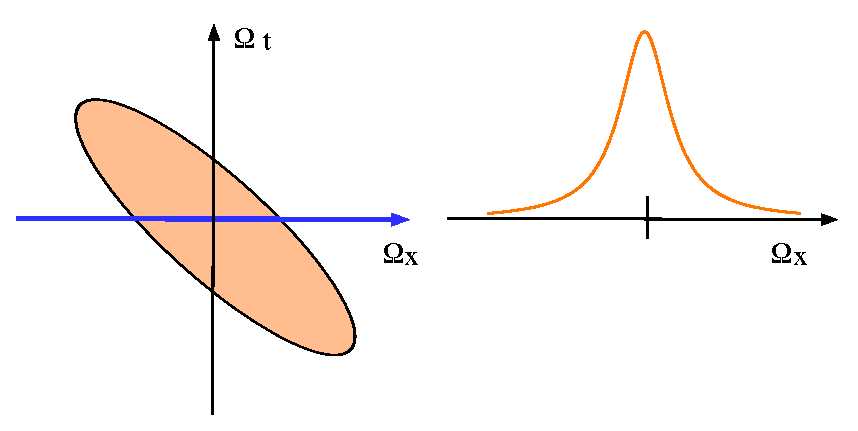
\includegraphics[width=0.65\textwidth]{figures/pt/slice-theorem}
	\caption{切片定理表明,原始函数沿某个维度的积分,等于其傅里叶变换频谱在该维度对应频率为0处的切片。这里表示沿$\Omega_t$轴的积分,对应为$\Omega_t=0$处的切片,即$\Omega_t$轴的直流分量}
	\label{f:pt-slice}
\end{figure}

有了上述定理,我们就可以开始用频率域分析来度量蒙特卡洛积分,因为每个像素的颜色值的采样还涉及对时间域(如运动模糊效果)和方向域(如聚焦效果)的积分,我们将看到采样涉及的走样怎样被用来表示蒙特卡洛积分的误差。设有1维积分$f$,根据上述的切片定理,该积分的真实值为其被积函数傅里叶变换在DC处的值:

\begin{equation}
	I={\rm \int}^{1}_0 f(x){\rm d}x=\hat{f}(0)
\end{equation}

\noindent 而根据蒙特卡洛积分,该积分估计(integral estimator)\mathindex{积分估计}{integral estimator}为$N$个随机数对应函数值的加权平均值:

\begin{equation}\label{eq:pt-setimator-sum}
	I_N=\sum w_i f(x_i)
\end{equation}

\noindent 我们可以将上述的数值模型用采样理论来表述:即首先按照一定的随机数分布对原始函数进行采样,然后求这些采样函数值的加权平均。与前面的采样理论类似,定义采样函数(sampling function)\mathindex{采样函数}{sampling function}为:

\begin{equation}
	S(x)=\sum w_i\delta(x-x_i)
\end{equation}

\noindent 其中,$S$也称为采样模式(sampling pattern)\mathindex{采样模式}{sampling pattern}。这里$\delta$是一个脉冲函数,即$S$只有在$x_i$处为非零值,如果$\sum w_i=1$,则$S$的积分值为1。不难看出,如果$x_i$是均匀分布的,则上述采样函数和第1章讨论的采样理论是完全一样的,即采样函数在被积函数的频率域拷贝相同长度的频谱。然而,在蒙特卡洛方法中,$x_i$是随机分布的,我们需要分析这种数值模型下的采样。

积分估计通常表示一些随机数值的和的形式,但是在上述定义了采样函数$S$之后,我们也可以将估计写为积分的形式,它和式\ref{eq:pt-setimator-sum}是等效的:

\begin{equation}\label{e:pt-sampling-1}
	I_N={\rm \int} S(x)f(x){\rm d}x
\end{equation}

\noindent 根据切片定理,上式可以转换为被积函数$S(x)f(x)$在其傅里叶变换空间DC处的值,根据傅里叶变换的属性,即两个函数内积的傅里叶变换等于两个函数傅里叶变换的卷积,即:

\begin{equation}
	\widehat{S\cdot f}=\hat{S}\otimes\hat{f}
\end{equation}

\noindent 这和第1章讨论的采样函数是一样的,即采样的过程是在原始函数$f$的傅里叶空间拷贝其频谱的过程,采样定理(sampling theorem)\mathindex{采样定理}{sampling theorem}说明,如果以均匀间隔进行采样,为了避免走样,采样函数至少应该以频率域最高频率2倍的采样率进行采样,原始函数才能被完美重建,即奈奎斯特采样率(Nyquist rate)\mathindex{奈奎斯特采样率}{Nyquist rate}。然而本节我们要讨论的是非均匀间隔采样,根据上式,式\ref{e:pt-sampling-1}表示的估计可以写为:

\begin{equation}
	I_N=\bigg(\hat{S}\otimes\hat{f}\bigg)(0)
\end{equation}

\noindent 上式可以总结为:蒙特卡洛积分的估计值等于其采样函数$S$的傅里叶变换与原始函数$f$的傅里叶变换的卷积在DC处(频率为0)的值,如图\ref{f:pt-sampling}中右下角的图中的红色粗线。

有了上述蒙特卡洛积分的频率域表述之后,我们应该怎样用频率域来分析或者表述蒙特卡洛估计的误差呢,因为这是本节的关键,我们希望找到走样(aliasing)\mathindex{走样}{aliasing}和蒙特卡洛方法之间的关系,从而可以通过避免走样而得到的采样分布来减少蒙特卡洛估计的误差。

根据这些分析结果,我们可以用频率域来表示蒙特卡洛估计的误差为:

\begin{equation}\label{e:pt-mc-aliasing}
	I_N-I=\hat{f}(0)-\bigg(\hat{S}\otimes\hat{f}\bigg)(0)
\end{equation}

\noindent 观察图\ref{f:pt-sampling},首先考虑如果$\sum w_i=1$,本节前面已经分析过此时$\hat{S}(0)=1$,那么式\ref{e:pt-mc-aliasing}中$\hat{f}$在DC处的拷贝将与$\hat{f}(0)$项(积分真实值)抵消,因此蒙特卡洛估计的误差来源于非DC处的$\hat{f}$频谱的拷贝在DC处的值,即此时蒙特卡洛估计的误差与采样形成的走样是等效的,它们在图\ref{f:pt-sampling}右下角的图中表现为其他非DC处的拷贝(绿色拷贝)与频率为0的红色线相交,因此采样走样导致了蒙特卡洛估计的误差,换句话说,采样模式与被积函数频谱之间的相关性导致了估计的误差。当然如果$\sum w_i\neq 0$时,蒙特卡洛估计的误差还来源于$\hat{f}$项本身。

\begin{figure}
	\sidecaption
	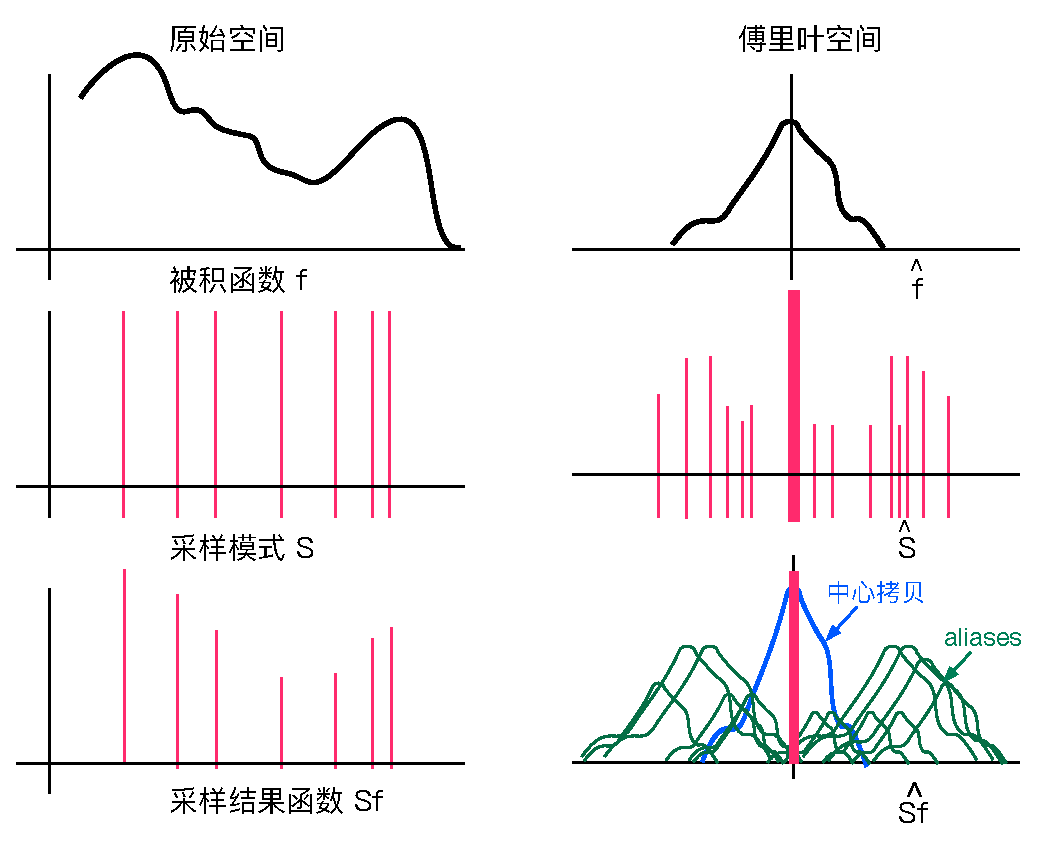
\includegraphics[width=0.65\textwidth]{figures/pt/sampling}
	\caption{采样表现为被积函数频谱$\hat{f}$按照采样模式的分布在频率域上的多个拷贝,传统的采样中采样函数是均匀分布的,在蒙特卡洛积分中,采样则是随机数形成不同的采样分布,如图中第二行的图分布表示一个非均匀采样函数在原始空间和傅里叶空间的分布。采样过程的走样来源于由于采样率太小而导致这些频谱的拷贝在DC处存在交集,如右下图所示(图片来自\cite{a:AFrequencyAnalysisofMonteCarloandotherNumericalIntegrationSchemes})}
	\label{f:pt-sampling}
\end{figure}

通过分析蒙特卡洛估计的误差与采样之间的关系,不难看出,适应性采样的策略就是要在尽可能减少每个区域采样密度分布的同时,避免被积函数频谱的各个拷贝在DC处相交。在原始空间采样密度越稀疏,则其在傅里叶空间的拷贝分布越密集,因此我们需要找到各个部分适当的采样密度来避免走样的产生,达到适应性采样的目标。

上述我们是在讨论一个积分值的估计的误差,然而通常我们对积分值并不感兴趣,而是通过计算积分值的蒙特卡洛方法来获取每个随机采样从而用于重建原始函数的分布,而从这个角度看,尽管整个积分值可能因为各个频谱拷贝在DC处不相交而结果是正确的,但是其函数的重建则会因为重建区域内多个频谱叠加出现走样,这也正是走样(aliasing)\mathindex{走样}{aliasing}的定义。因此传统的采样定理(sampling theorem)\mathindex{采样定理}{sampling theorem}要求,采样率必须大于原始函数傅里叶变换频谱的最大频率的两倍,这样才能保证原始函数的完美重建。

然而因为积分值本身的估计只要求其频谱拷贝在DC处不相交,因此针对积分值估计,例如下一节将要讨论的针对时间域和方向域的积分,传统的采样定理的要求则可以放松,即只要满足采样率只需要大于最大频率即可以保证积分值的估计不会出现走样,这即是奈奎斯特采样率(Nyquist rate)\mathindex{奈奎斯特采样率}{Nyquist rate}的一半,这称为修正的采样定理(revised sampling theorem)\mathindex{修正的采样定理}{revised sampling theorem},我们将会将此定理运用于下一节适应性采样中涉及的积分值估计的过程,读者可以参考\cite{a:AFrequencyAnalysisofMonteCarloandotherNumericalIntegrationSchemes,a:5DCovarianceTracingforEfficientDefocusandMotionBlur}等阅读阅读更详细的相关信息。





\subsubsection{协方差追踪在适应性采样中的运用}
有了前面这些基础条件及原理,我们就可以更好地理解利用频率域分析方法来实现适应性采样和适应性重建,本节我们将使用第\ref{sec:pt-covariance-tracing}讨论的协方差追踪来实现适应性采样和适应性重建。

首先要明白的是,我们很难在图像的全局区域内进行适应性采样,例如我们很难选取一个任意尺寸的区域进行分析从而实现适应性采样。本节我们讨论的方法通常都是以一个像素作为适应性采样分析的范围,即是我们对每个像素进行分析,计算出该像素需要的采样数量,但是我们的重建过滤器是可以跨域一个像素区域的,参见本节后面的内容。

适应性采样(adaptive sampling)\myindex{适应性采样}{adaptive sampling}涉及将整个采样的过程划分为多个迭代的过程,这样便可以使用适当的方法通过分析前序采样过程或结果来计算出后续采样过程使用的采样密度分布。然而,由于先验方法需要跟踪整个光线传输的过程,为了提高计算效率,这些方法通常不会对整个光线追踪过程进行频率域分析,而是采用一个简化的处理:由于直接光照对图像光照的贡献是最大的,因此这些方法仅通过对直接光照进行局部分析来近似整个路径空间光照的分布。

\begin{figure}
\begin{fullwidth}
	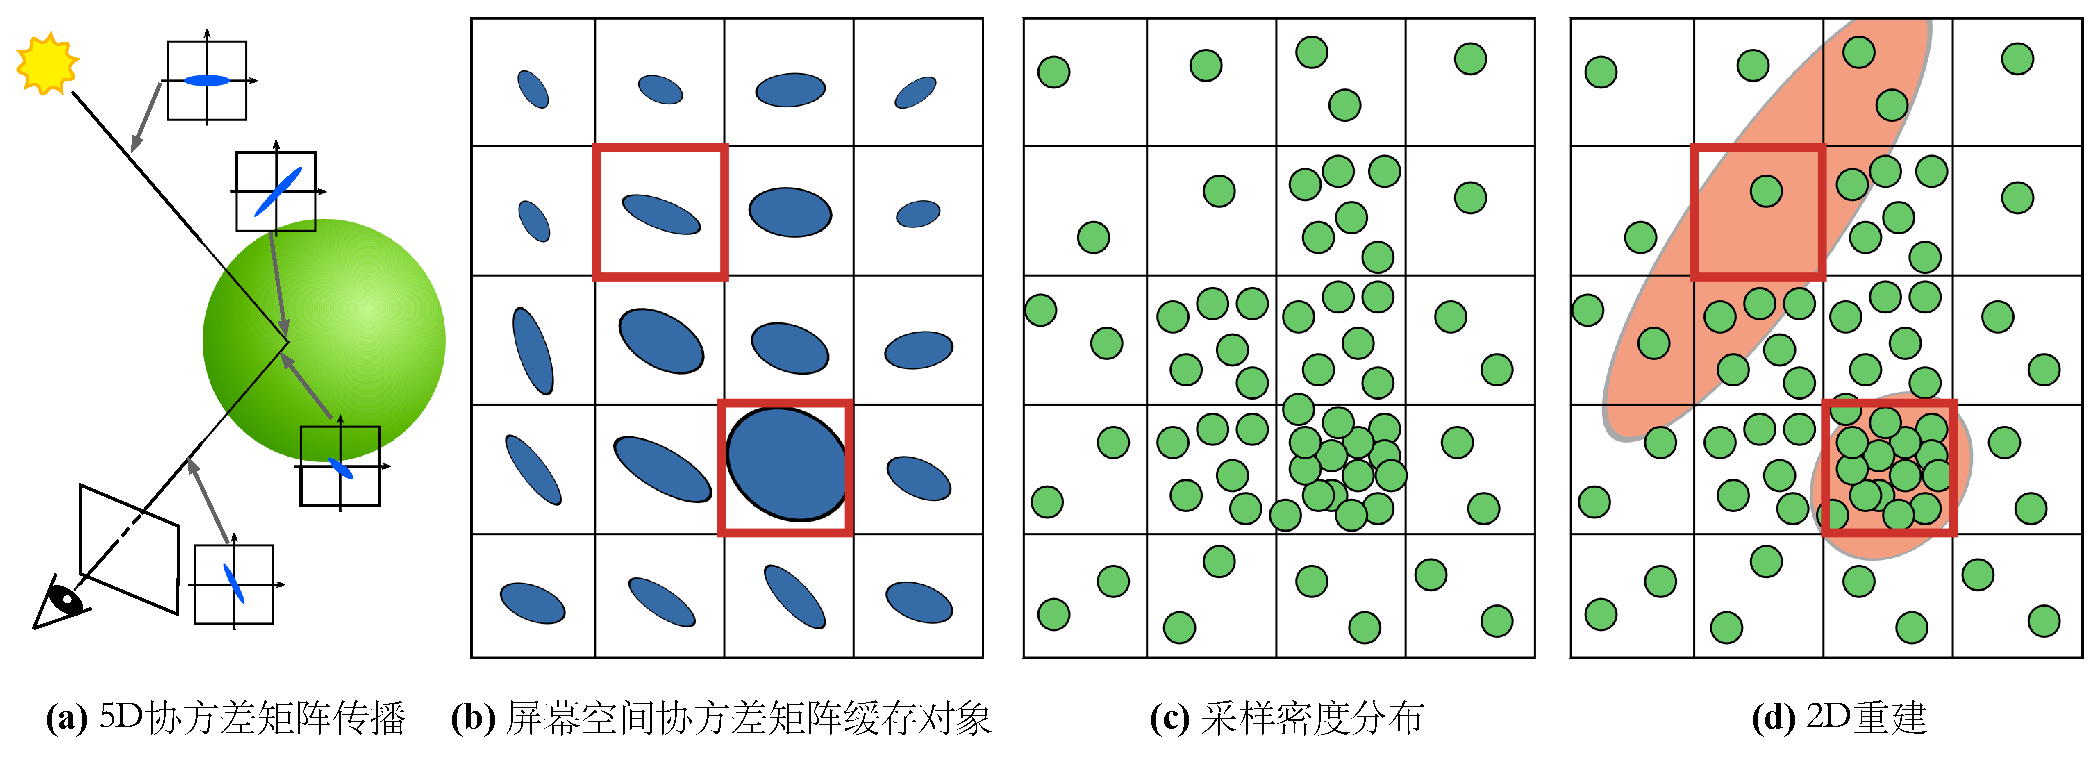
\includegraphics[width=1.\thewidth]{figures/pt/adaptive-sampling}
	\caption{利用协方差追踪的适应性采样和重建方法首先通过发射一些稀疏的直接光照来近似图像分布,并跟踪这些光照路径的协方差矩阵来帮助计算每个像素的采样密度分布和重建过滤器(图片来自\cite{a:5DCovarianceTracingforEfficientDefocusandMotionBlur})}
	\label{f:pt-adaptive-sampling}
\end{fullwidth}
\end{figure}

\cite{a:5DCovarianceTracingforEfficientDefocusandMotionBlur}介绍的利用协方差追踪实现适应性采样和适应性重建的方法首先从摄像机像图像平面发射一定数量均匀的光线,然后将这些光线与场景的交点与光源相连形成直接光照路径,然后通过该路径沿相反(即由光源到摄像机)的方向发射并跟踪局部光照场的协方差矩阵,如图\ref{f:pt-adaptive-sampling}(a)所示,最后这些协方差矩阵投射到图像屏幕并利用这些协方差矩阵来实现适应性采样和适应性重建。这主要包含以下四步(如图\ref{f:pt-adaptive-sampling}所示):

\begin{enumerate}
	\item 首先,将由光源像摄像机发射得协方差矩阵在每个像素位置进行累加,这形成一个2D的协方差缓存对象(covariance matrix buffer)\mathindex{协方差缓存对象}{covariance matrix buffer},每个协方差是一个5D(空间-方向-时间)的函数分布,如图\ref{f:pt-adaptive-sampling}(b)所示。
	\item 然后,利用每个像素的协方差矩阵计算该像素范围内针对5D局部光照场分布的采样密度,以及一个2D的重建过滤器,如图\ref{f:pt-adaptive-sampling}(c)所示。
	\item 接着,对每个像素按照上一步得出的采样密度进行采样,并将这些采样的结果存储在一个2D的数据结构中。
	\item 最后,对于每个像素,我们对处于其对应重建过滤器区域内的所有采样进行加权计算,这可能包括来自附近相邻像素的采样值,如图\ref{f:pt-adaptive-sampling}(d)所示。
\end{enumerate}

对于协方差矩阵的累加,根据协方差矩阵每一项的定义,其为分布函数傅里叶变换振幅的积分,不难推断出两个频谱和的协方差矩阵等于其各自协方差矩阵的和,\cite{a:5DCovarianceTracingforEfficientDefocusandMotionBlur}提出的近似协方差加权和为(如图\ref{f:pt-covariance-sum}所示):

\begin{equation}
 \mathsmaller{\sum}\simeq\mathlarger{\sum_{x\in p}} \cfrac{E_i}{E} \mathsmaller{\sum\nolimits_i}
\end{equation}

\noindent 上式中$E_i$表示第$i$个采样的辐射亮度,$E$表示像素$p$内所有直接光采样辐射亮度的总和。

\begin{figure}
\sidecaption
	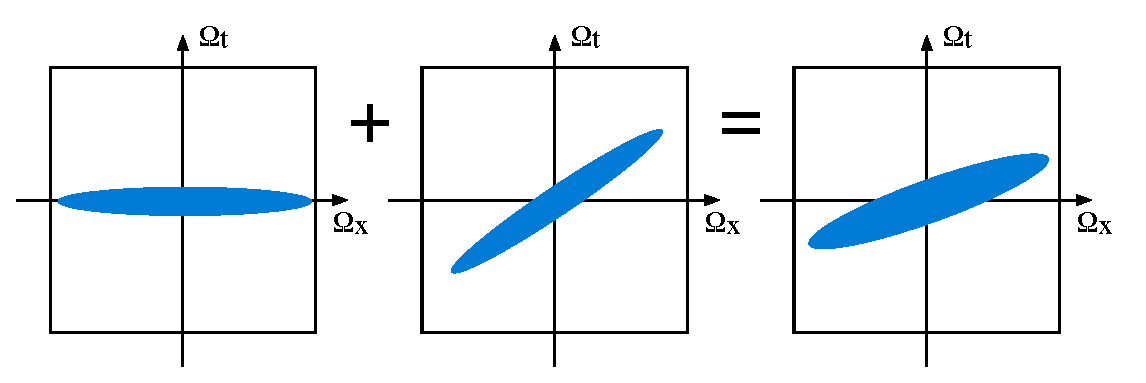
\includegraphics[width=0.65\textwidth]{figures/pt/covariance-sum}
	\caption{两个协方差矩阵的和,这里图示的是协方差对应的椭圆形高斯近似形状}
	\label{f:pt-covariance-sum}
\end{figure}

我们需要计算5D空间内采样密度分布,因此我们直接通过5D的协方差矩阵来计算采样密度,否则我们还需要对像素内的采样在时间域和方向域做积分计算。为了在5D空间内进行采样,我们可以将采样理论运用于5D空间,即采样函数$S(x)f(x)$是一个5D函数,如图\ref{f:pt-sampling-theorem}上面一行表示原始空间内采样模式和被积函数的乘积,从上一节的内容可知,这实际上是傅里叶空间的一个卷积,即$\hat{f}$在频率域的多个拷贝,如图\ref{f:pt-sampling-theorem}下面一行表示傅里叶空间采样函数和被积函数频谱的卷积(拷贝)。

\begin{figure}
\sidecaption
	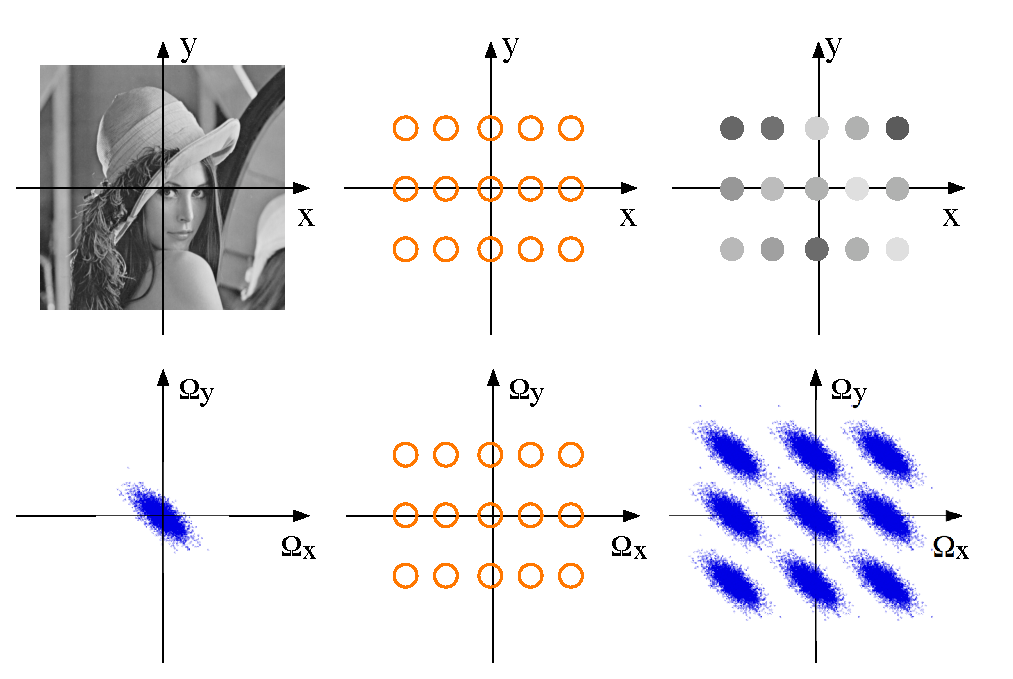
\includegraphics[width=0.65\textwidth]{figures/pt/sampling-theorem}
	\caption{采样理论表面,原始空间内(上行)被积函数与采样模式的乘积对应于傅里叶变换空间内对应函数频谱的卷积,由于采样函数脉冲函数,其傅里叶变换仍为脉冲函数,所以采样等效于傅里叶空间内被积函数频谱的多个拷贝(下行)。采样理论就是要保证这些拷贝之间不会相互重叠导致走样}
	\label{f:pt-sampling-theorem}
\end{figure}

求积分的问题实际上是求$(\hat{S}\otimes\hat{f})(0)$的值,所以我们的目标是保证该值不含走样,也即是我们应该保证每个拷贝不相互重叠,这需要计算出5D空间内频谱的“体积”,以决定以多大的间隔对原始函数进行采样才不会导致拷贝之间的重叠。

矩阵的雅可比行列式\mathindex{雅可比行列式来}{Jacobian determinant}提供了关于原始频谱体积的度量,它表示一个单位超立方体(unit hypercube)\myindex{单位超立方体}{unit hypercube}体积随该矩阵变换的变化(variation),因此协方差矩阵的行列式提供了采样密度的信息,然而需要注意的是,协方差矩阵的每一项度量的是类似于方差(而非标准差)的属性,即是某个维度变化的平方,所以我们应该使用协方差矩阵行列式的平方根来度量单位超立方体体积的变化,像素$p$内的采样密度应该正比于该像素5D协方差矩阵行列式的平方根,所以采样密度可表示为:

\begin{equation}
	N_p=k\sqrt{|\mathsmaller{\sum}|}
\end{equation}

\noindent 上式中$k$是一个常数,它可以使我们将$N_p$表示为整个图像采样数量的一个分数,$N_p$并不是一个绝对数量,而是被用来计算每个像素采样密度的一个比例。当计算出各个像素的采样密度分布之后,再使用完整的路径追踪算法按这些采样密度分布对整个路径空间进行采样,并将这些采样结果存储在一个2D的数据结构以便后续的重建。

为了避免用高维的数据结构存储采样,\cite{a:5DCovarianceTracingforEfficientDefocusandMotionBlur}使用2D的协方差矩阵来计算重建过滤器,这通过使用上一节讨论的切片定理来实现。为了得出2D的协方差,首先将局部光照场对方向域和时间域进行积分,得到:

\begin{equation}
	l(x,y)={\rm \int}_{u,v,t}l(x,y,u,v,t)ws(u,v,t){\rm d}u{\rm d}v{\rm d}t
\end{equation}

\noindent 这里$ws$表示聚焦范围\footnote{对于聚焦效果,其方向域相当于透镜上的位置。}和摄像机快门时间的乘积,这等效于其傅里叶变换空间两个函数卷积在DC处的值:

\begin{equation}
	\hat{l}(\Omega_x,\Omega_y)=[\hat{l}\otimes ws](0,0,0)
\end{equation}

\noindent 为了执行过滤,我们需要基于采样的位置来对采样进行加权平均,这里使用高斯过滤器(Gaussian filter)\myindex{高斯过滤器}{Gaussian filter}来进行过滤。

直观上,每个像素处协方差矩阵对应的频谱面积越大,表示该区域的频率变化越大,则该像素使用的采样数量越多,因此在图像空间对该像素应该使用更小的过滤范围;相反,如果协方差矩阵对应的频谱面积越小,则该区域的变化约小,使用的采样越稀疏,因此在图像空间应该使用更大范围的过滤器。这也是选择高斯过滤器的原因之一,因为高斯过滤器的局部变化在原始空间和傅里叶空间是相反的。

在数学形式上,\cite{a:Fast4DShearedFilteringforInteractiveRenderingofDistributionEffects}将一个2D过滤器表示两个1D高斯过滤器的乘积:

\begin{equation}
	h(x,y)={\rm e}^{-k_x(x-x_0)^{2}}{\rm e}^{-k_y(y-y_0(x,x_0))^{2}}
\end{equation}

\noindent 这里$y_0=\eta(x-x_0)$表示$y$轴过滤器的中心,这里的过滤器使用和协方差矩阵提供的频谱的图像空间相同的形状来度量,为了计算图像空间的高斯过滤器,这需要计算协方差矩阵的逆矩阵,因此上式结合协方差矩阵可以变化为:

\begin{equation}
	h(x,y)={\rm e}^{-[x-x_0,y]\sum\nolimits^{-1}[x-x_0,t]^{T}},\text{ 其中 }\mathsmaller{\sum\nolimits^{-1}}=\begin{bmatrix}
		k_x+k_y & \eta k_y\\
		\eta k_y &k_y
	\end{bmatrix}
\end{equation}


本节我们讨论了降噪技术中的先验方法,即通过跟踪光照传输的局部特征(变化)来推导适应性采样的概率密度分布和适应性重建的过滤器。特别地,我们以协方差为例分析了相关的思路,过程及原理,
\cite{a:ALocalFrequencyAnalysisofLightScatteringandAbsorption}还讨论了基于协方差追踪的针对参与介质的处理,这里不再讨论。同时,其他的局部频率域分析方法或者一些基于几何特征(如微分几何)的方法仍然可以作为先验降噪技术的基本工具,读者可以结合本节的思路进行相应理解和学习。







\subsection{后验方法}
在上一节中,我们讨论了降噪技术中的先验方法,它通过跟踪屏幕空间一个像素尺寸大小的局部光照场随着光线传输的变化来估计图像的局部变化特征,从而对图像进行适应性采样和适应性重建。由于对局部光照场的追踪考虑了直线传输,阴影遮挡,BRDF反射函数,运动,聚焦等效果,因此先验方法可以较准确地反应图像的局部变化特征。

除此之外,我们也可以通过直接对图像空间进行分析来得出图像的局部特征变化,这就是本节讨论的后验方法(a posteriori methods)\myindex{后验方法}{a posteriori methods}。图像空间(image space)\myindex{图像空间}{image space}的方法在思路上和路径空间的方法是不一致的,在图像空间,唯一可用的数据是采样结果,即相当于是服从图像分布的一些随机数,为了分析图像的局部特征,我们可以通过分析这些随机数的误差分布来达到。因为直观上,某个区域的误差越大,通常该区域的频率变化越高,则该区域需要更多的采样,反之亦然。所以误差分析是后验方法的核心。由于后验方法不需要知道样本使用什么样的采样算法获得,所以很容易集成到现有渲染解决方案当中。此外,图像空间的后验方法要比路径空间的先验方法在性能上要高效的多。

本节我们将首先在第\ref{sec:pt-adaptive-framework}节讨论图像空间降噪技术的一般原理框架,然后在后面讨论具体某些环节的一些技术选择,第\ref{sec:pt-image-processing}节讨论一些图像处理中的方法,第\ref{sec:pt-feature-filtering}节讨论利用一些辅助信息(如深度值等)来辅助过滤技术,第\ref{sec:pt-first-order-regression}则介绍更精确的一阶回归方法。







\subsubsection{图像空间降噪技术的基本框架}\label{sec:pt-adaptive-framework}
渲染图像的每个局部区域的方差通常是变化的\footnote{回想方差只和样本本身相关,与真实值无关,因此每个局部范围内的样本可能具有不同的方差。},适应性采样的目的就是要通过让方差比较大的部分区域获得更多的采样数量,来降低方差。上节我们通过分析走样来分析局部方差大小,在那里将方差表示为走样,从而通过降低走样来减少方差,本节则将直接根据随机数的特征来分析图像局部区域的误差分布。

降噪技术的主要思路是将采样的过程划分成多个迭代的过程,对于图像空间的降噪技术,每个迭代由以下两个步骤组成,如图\ref{f:pt-demoising}所示,即:

\begin{itemize}
	\item \textbf{适应性采样 } 当采样过程进行第一个迭代时,对整个图像空间使用均匀分布的采样;从第二个迭代开始,它首先从上一个迭代中输出的重建图像(filtered image)\myindex{重建图像}{filtered image}计算出一个误差估计,然后根据这个误差分布计算出一个采样密度分布,从而根据这个采样密度分布进行适应性路径采样。
	\item \textbf{适应性重建 } 对于每一个迭代中输入的稀疏的采样集合,由于这些采样包含较大的方差(噪点), 为了分析这些采样的误差分布,首先要对其进行适应性过滤(否则其误差估计结果会被较大的方差影响),然后将过滤后的图像输出到适应性采样阶段用于计算残留的误差。
\end{itemize}

\begin{figure}
	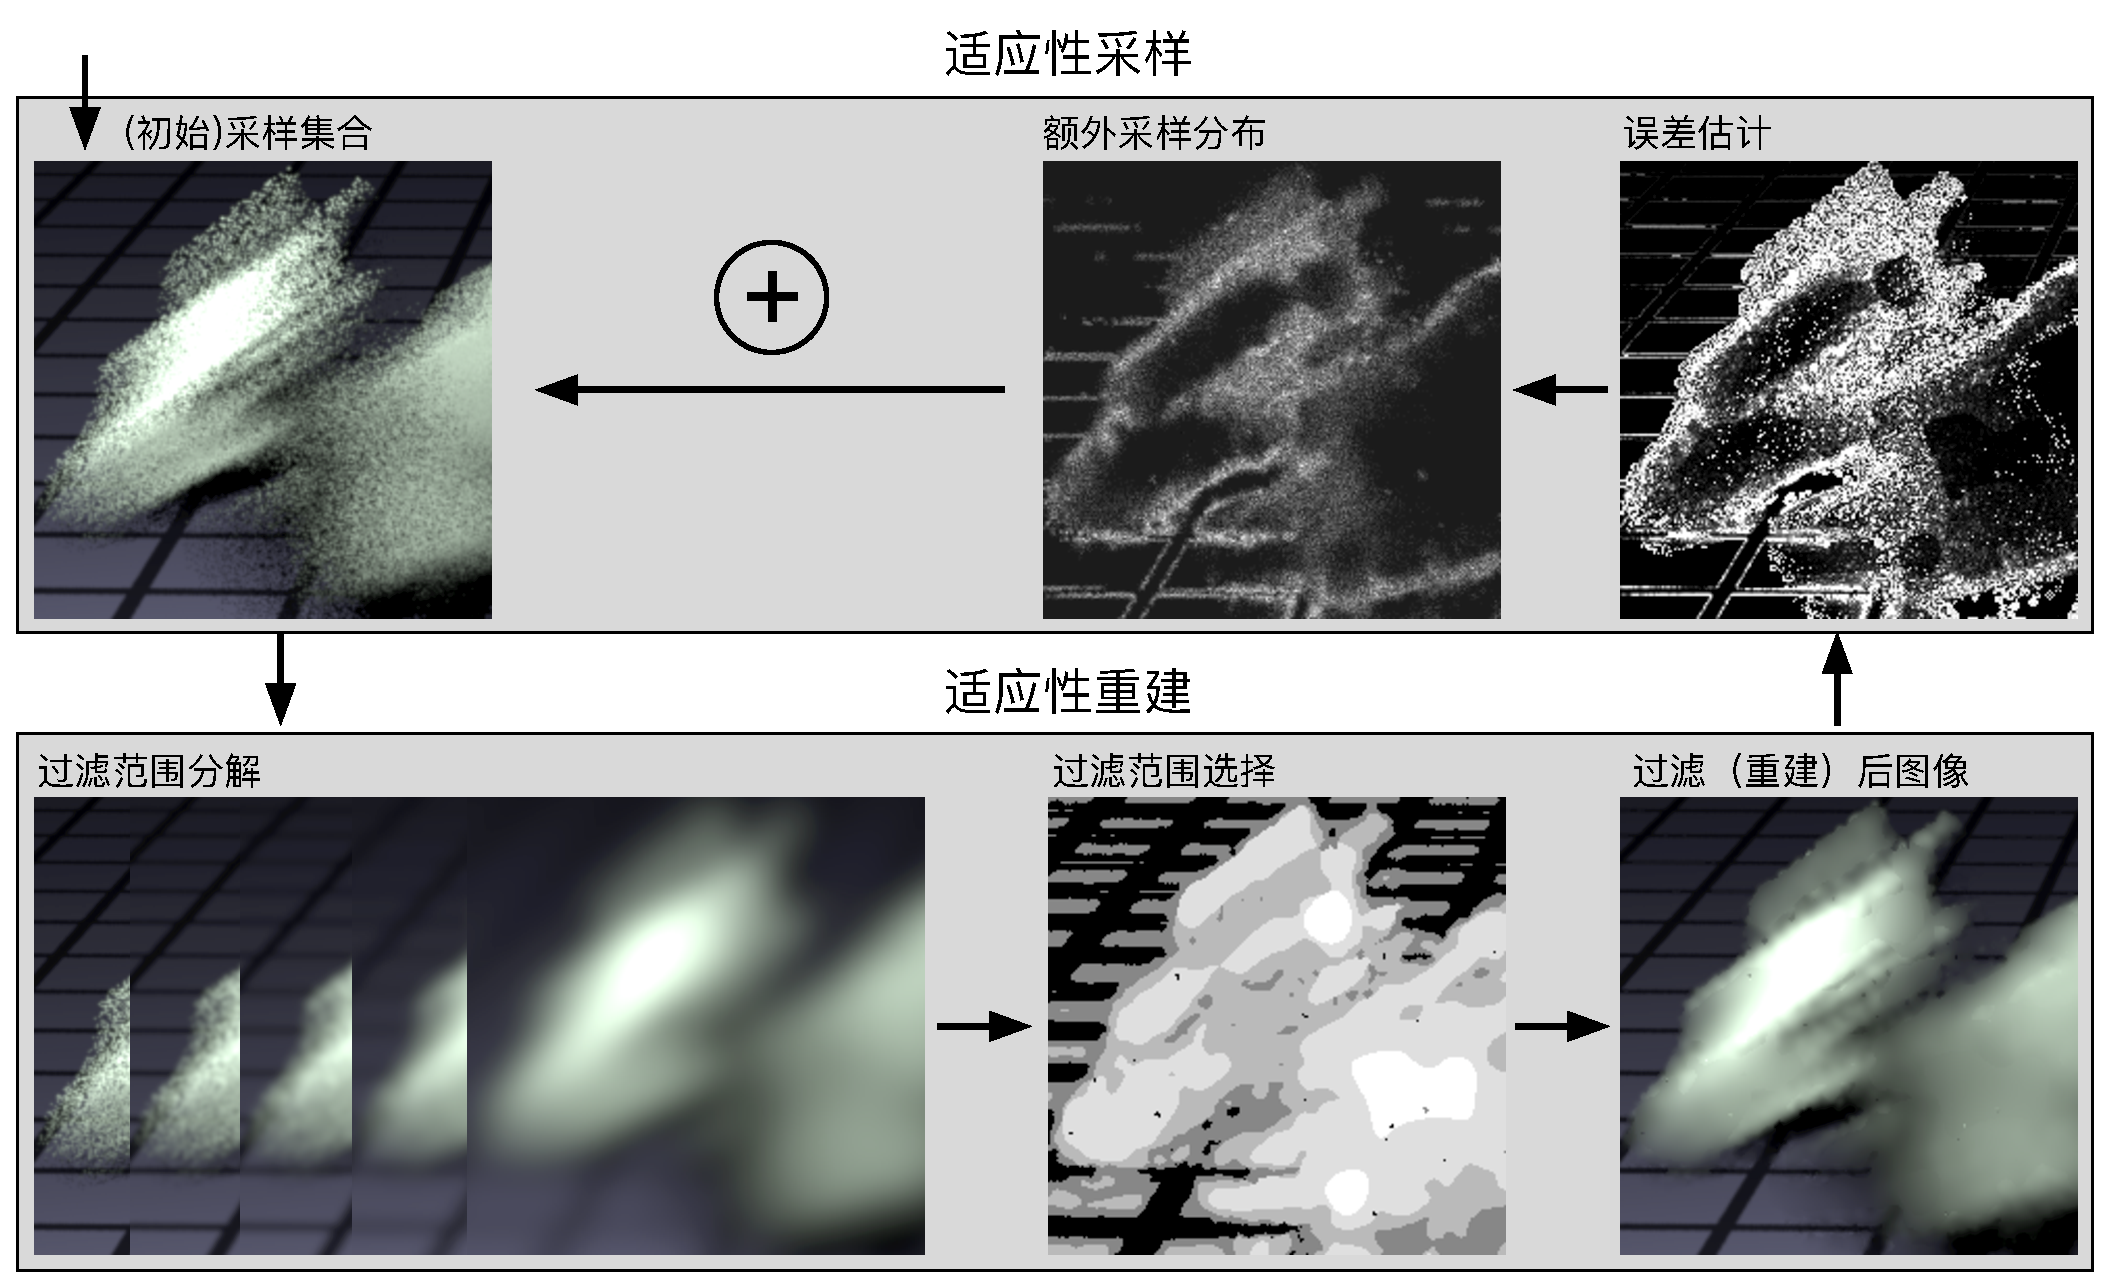
\includegraphics[width=1.0\textwidth]{figures/pt/denoising}
	\caption{图像空间降噪技术的基本框架,在每个迭代中它首先对输入的稀疏带有较大方差的采样集合进行适应性过滤以降低方差,然后计算过滤后图像中残留的误差分布来得出采样密度分布,从而用于指导下一迭代过程的适应性采样(图片来自\cite{a:AdaptiveSamplingandReconstructionusingGreedyErrorMinimization})}
	\label{f:pt-demoising}
\end{figure}

上述的过程描述非常简洁,然而这里面包含非常多的逻辑以及一些容易令人困惑的概念,本节的首要任务是理解这些逻辑,然后在后面的内容中将讨论当前工业中每个步骤一些主流的实现方法。

首先,为什么要对输入的稀疏采样集合进行过滤后(而不是直接)计算其误差分布?降噪技术的其中一个目标便是在减少路径采样的样本数量(从而也是减少计算的时间)的同时提高渲染图像的质量,由于样本数量更少,每一个迭代中输入的采样集合带有较大的方差,因此使用这些样本计算出的误差分布本身也会带有较大的误差,不利于更好地指导适应性采样。因此,我们必须首先减少输入样本集合的误差,而过滤便是减少误差的常用方法。

其次,对输入集合的过滤必须是适应性的,即针对不同的区域使用不同范围的过滤器。使用全局统一范围的过滤器会使得有些方差比较小的区域过于模糊(参见本节后面的内容),而这会增加过滤后图像的偏差,从而可能导致总的误差(如均方差)增大,也不利于计算采样密度分布。常用比较高效简单的方法是使用一些具有不同过滤范围(filtering bandwith)\myindex{过滤范围}{filtering bandwith}的过滤器对每个像素进行过滤,然后选择其误差最小的过滤器作为最终使用的过滤器,这一过程称为范围选择(bandwidth selection),如图\ref{f:pt-demoising}左下部分所示。在图像空间的降噪技术中,选择什么样的过滤器,以及使用怎样的范围选择策略是实践中的重要内容。

最后,对于重建后的图像,由于过滤导致其具有偏差,同时还残留一部分方差,所以我们还需要对最终图像进行误差估计,通常是使用均方差作为标准,其计算出的结果才用于生成采样密度分布。

以下,我们再介绍理解本节内容的两个重要知识点。






\paragraph{方差,偏差以及过滤之间的关系}
为了更好地理解本节的内容,我们有必要了解一下过滤对方差(variance)\mathindex{方差}{variance}和偏差(bias)\mathindex{偏差}{bias}的影响。我们通常用均方差(mean squared error,MSE)\mathindex{均方差}{mean squared error}来衡量一个估计的误差,在第\ref{sec:pt-bias-consistency}节我们已经介绍过,它表示一个估计与其真实值之差的平方的期望,这里为了方便重写其公式如下:

\begin{equation}
\begin{aligned}
	MSE(I_N)=&E[(I_N-I)^2]\\
	        =&E[(I_N-E[I_N])^2]+(E[I_N]-I)^2\\
	        =&Var+Bias^{2}
\end{aligned}
\end{equation}

\noindent 这里$I$为真实值,$I_N$为其估计。由此可以看出,方差反应的是局部特征(其值只与局部样本有关,与真实值无关),而偏差反应的是系统特征(其值与真实值有关),一个估计不管方差多大,只要它的全部分布都是可能被采样到的,随着采样数量的积累,估计总会慢慢趋近于真实值,即估计是无偏的。但是,如果某些样本永远不可能被采样到,就会产生系统偏差,导致极限情况下的期望值不等于其真实值,这样的估计就是有偏的。

由此我们可以得出一个推论,任何导致原始函数某些分布区域消失的操作都可能增加估计的偏差。

我们知道,基本的路径采样是无偏的(unbiased)\myindex{无偏的}{unbiased},其均方差仅由方差组成。方差表示的是局部区域内样本和其期望(均值)之间的差异,较大的方差通常意味着该区域的频率变化较大,因此方差可以通过过滤来减小。然而,过滤在减小样本方差的同时,我们看到它平滑了频率分布,即是使得某些频率域被抹除了,这相当于使得原始函数某些高频区域不能被采样。因此,过滤导致或者增加了偏差,从这个角度来看,偏差对应于图像的模糊强度(blurriness)\myindex{模糊强度}{blurriness}。

所以,对于过滤操作,虽然更大的过滤范围消除了更多的方差,但是它同时也增加了偏差,因此总的均方差也可能会增加,方差和偏差随着过滤范围的变化关系如图\ref{f:pt-var-and-bias}所示,方差随着过滤范围的增加而减少,偏差则随着过滤范围的增加而增加。需要注意的是,图\ref{f:pt-var-and-bias}中过滤范围值的起点为1个像素大小,此时每个像素周围的像素并没有被混合近该像素中,这即是路径采样算法默认使用的过滤器,这称为像素过滤器(pixel filter)\myindex{像素过滤器}{pixel filter},在该过滤范围下其偏差为0。

\begin{figure}
	\sidecaption
	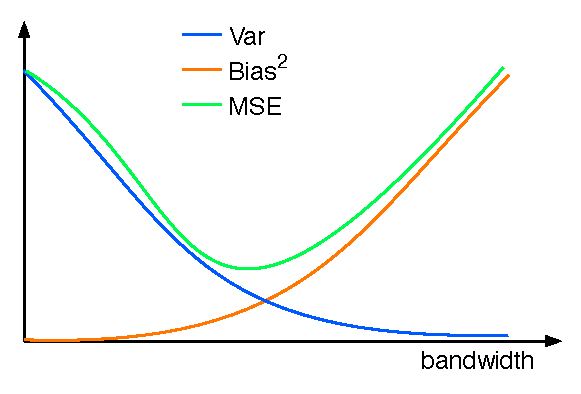
\includegraphics[width=0.5\textwidth]{figures/pt/var-and-bias.eps}
	\caption{过滤同时影响着方差和偏差,方差随着过滤范围的增加而减少,偏差随着过滤范围的增加而增加,因此我们必须对不同的区域选择适当的过滤范围使得其均方差最小}
	\label{f:pt-var-and-bias}
\end{figure}

因此我们必须选择适当的过滤范围,其范围选择的依据应该是使得均方差的值最小,接下来将讨论降噪技术中过滤范围选择的一些概念和方法。





\paragraph{过滤范围选择}
通过上面的分析,过滤导致偏差\footnote{开始学习适应性采样和过滤时会产生的一个疑惑是,既然过滤导致偏差,那么降噪技术的运用会使路径采样变为有偏的吗?这里当然不会,适应性过滤仅被用来计算一个采样密度分布图,它并不会对所有样本产生任何影响,最终图像还是通过所有原始样本在像素内的平均值(即像素过滤器)生成的,所以其结果仍然是无偏的。},因此过滤范围的选择必须平衡两个相冲突的目标:减少方差和阻止偏差(过度模糊),这样才能使得过滤后图像的均方差最小。

要想知道过滤对于均方差的影响,必须首先将过滤器作用于采样采样集合,所以很显然我们不可能通过任何途径在过滤前能够计算出一个最优的过滤范围,而只有对其过滤的结果进行分析来指导过滤范围的选择。为了避免让用户手动输入一些参数来进行过滤范围的调整,在降噪技术中一般通过两种方式来进行过滤范围的自动选择:一种是直接估计,这些方法使用统计分析\cite{a:OnFilteringtheNoisefromtheRandomParametersinMonteCarloRendering}或机器学习\cite{a:AmachinelearningapproachforfilteringMonteCarlonoise}来指导选择过滤范围,在实践中这些方法的计算复杂度通常比较高;另一种比较常用且高效的方法称为基于选择的估计(selection-based estimate)\myindex{基于选择的估计}{selection-based estimate},这些方法通常预先定义一些固定范围的过滤器,然后对比选择均方差最小的过滤器,以下以及本节后面我们将重点讨论此种方法。

基于选择的估计方法有两个问题需要解决,首先是确定选择使用什么样的过滤器,\cite{a:AdaptiveSamplingandReconstructionusingGreedyErrorMinimization}选择使用高斯过滤器,高斯过滤器是各向同性的过滤器,每个级别的过滤器被均匀缩放,因此每个预定义的范围就是一个缩放系数,其中最小的缩放因子为1,它等效于基本路径采样中的像素过滤器,因此是无偏的,同时也是精细度最高的过滤器。随着缩放因子增大,过滤的结果越模糊,或者平滑。

定义好一些由精细到模糊的过滤器之后,剩下的问题是使用什么样的方式对每个过滤器进行误差估计。由于均方差由方差和偏差的平方构成,而偏差的计算要求必须知道真实值,这个值显然是未知的,因此很难通过直接计算均方差来进行过滤范围选择。后面我们将讨论一些比较高级直接估计均方差的方法,这里为了理解过滤范围选择的概念,我们首先介绍\cite{a:AdaptiveSamplingandReconstructionusingGreedyErrorMinimization}提供的一种比较简单的选择方法。

\begin{figure}
	\sidecaption
	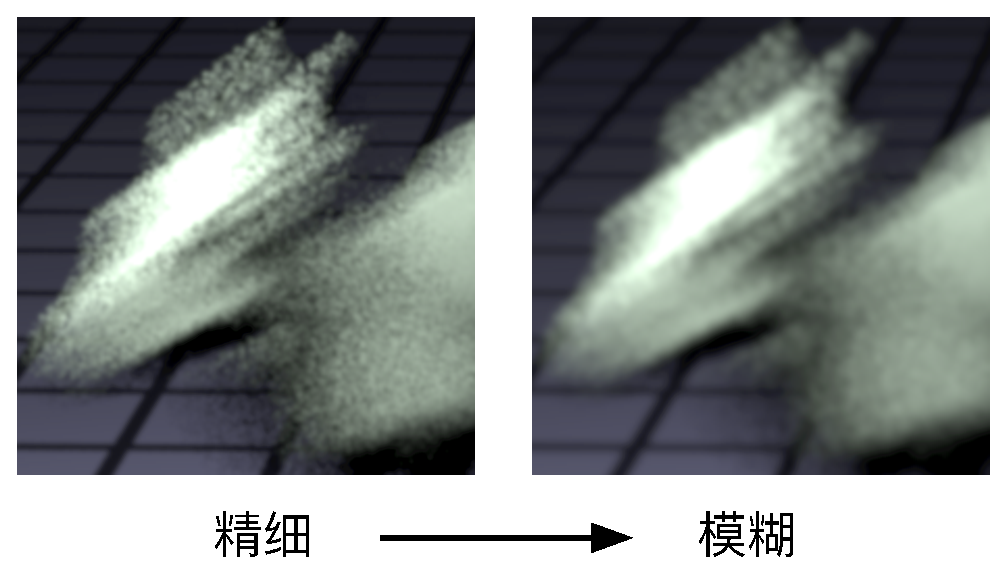
\includegraphics[width=0.45\textwidth]{figures/pt/fine-to-coarse}
	\caption{对每个像素按照由精细到模糊的顺序进行过滤,并计算其均方差,根据单调性,只要相邻两个均方差之差为正则停止遍历,就可以找到最小均方差的过滤器(图片来自\cite{a:AdaptiveSamplingandReconstructionusingGreedyErrorMinimization})}
	\label{f:pt-fine-to-coarse}
\end{figure}

如图\ref{f:pt-var-and-bias}所示,随着过滤范围的增加,方差呈现单调递减,偏差呈现单调递增的趋势,而总的均方差呈现先减少后增加的趋势。根据这种单调性,则可以很容易地通过对过滤器进行从精细到模糊的方向进行遍历比较以寻找最小均方差。因此,他们首先对预制过滤器按照从精细到模糊的顺序排序,如图\ref{f:pt-fine-to-coarse}所示,然后分别对每个像素按照这个顺序进行过滤,并对每两个相邻的过滤结果进行方差比较,直到:

\begin{equation}
	\Delta MSE(fine\rightarrow coarse)=MSE[c]-MSE[f]>0
\end{equation}

\noindent 时停止,这里$f$表示更精细(fine)的过滤器,而$c$表示更模糊(coarse)的过滤器。

那怎样估算过滤器的均方差呢?虽然偏差的计算需要知道真实值,但是方差只与当前使用的样本有关(当前样本的期望),它不需要知道真实值,因此很容易计算得出。对于偏差,由于不能直接通过样本计算得出,\cite{a:AdaptiveSamplingandReconstructionusingGreedyErrorMinimization}使用一个二次方近似来计算偏差。

这里我们不再提供原论文的近似形式,因为后面会介绍更好的方法(如SURE)。这里读者仅需要了解过滤范围选择的概念和思路,即首先提供一些预制的不同范围的过滤器,然后分别对每个像素使用这些过滤器,并通过某种方式计算过滤后的均方差来选择均方差最小的过滤器,从而达到过滤范围选择的目的。需要注意的是,这里的方差和偏差都是针对每个像素的,它们的计算使用的样本是每个过滤器覆盖的全部样本值。经过范围筛选后的过滤范围分布如图\ref{f:pt-demoising}下行中间小图或者图\ref{f:pt-denoising-results}(b)所示。

除了使用过滤器进行近似,\cite{a:AdaptiveWaveletRendering}还通过对输入集合使用小波(wavelet)\mathindex{小波}{wavelet}近似来估计误差,小波分析是一种将信号分解为多个不同分辨率的信号,然后每个分辨率能够反映信号中不同程度的精细度,我们将在本书后面的章节详细讨论小波分析,这里仅了解它也可以用来作为一种选择过滤范围的思路。另外,除了将均方差用作一种局部特征判断的度量(metric),其他一些度量方法也被使用,例如\cite{a:BoostingMonteCarloRenderingbyRayHistogramFusion}使用直方图来进行度量。






\paragraph{采样分配}
我们的目标是根据图像的局部误差特征计算出一个采样密度分布,用于指导下一迭代过程中的适应性采样。

上述的适应性过滤的目的在于减少稀疏采样集合的误差,使得每个像素使用的过滤器对应的均方差最小。在经过适应性过滤之后,我们得到一个过滤后的图像,如图\ref{f:pt-demoising}中右下角的小图,该图还带有残留的方差以及由于过滤导致的偏差,通常在计算采样密度之前还需要使用其他方法来计算最终的误差估计(error estimation)\myindex{误差估计}{error estimation},我们将在后面介绍一些具体方法,这里主要是理解怎样基于过滤后图像的误差估计计算出采样密度分布。

首先,有一个可能容易引起误解的概念,即用上述得到的误差估计直接推导出采样密度分布,因为误差越大的地方显然需要更多的采样。但是这个想法是错误的,因为这里每个像素的误差估计是通过该像素使用的过滤器范围来的采样来估计计算得出的,即是该过滤器范围内的像素对应的采样都对该像素有影响,除非每个像素的误差仅有该像素内的采样计算得出才可以直接使用误差估计作为采样密度分布的依据。因此,这里重点是要根据过滤范围计算出该范围内的采样对该像素有着怎样的影响。

\begin{figure}
	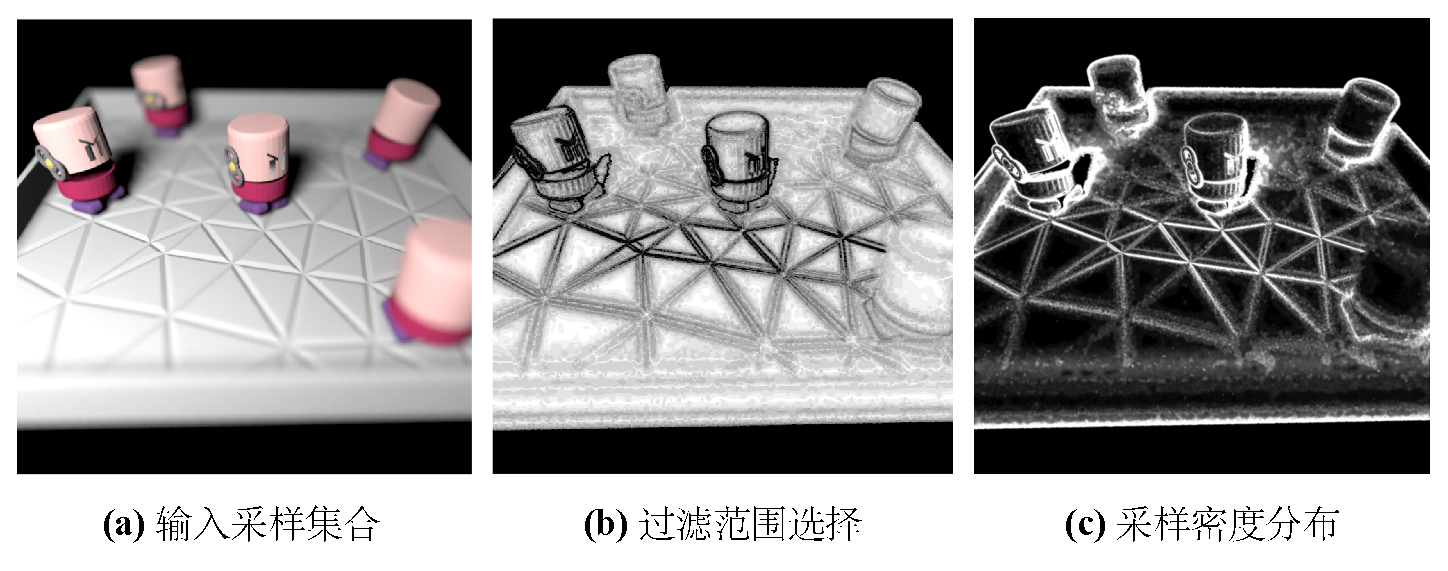
\includegraphics[width=1.0\textwidth]{figures/pt/denoising-results}
	\caption{过滤范围选择产生的每像素范围分布(d),以及对应的每像素采样数量分布图(c),该场景(a)同时包含景深效果和面积光源(图片来自\cite{a:AdaptiveRenderingaposteriorimethods})}
	\label{f:pt-denoising-results}
\end{figure}

在实践中通常使用相对均方差(relative MSE)\myindex{相对均方差}{relative MSE},设像素$p$处的相对均方差为$E(p)$,因为一个像素的方差跟它的样本数量是成反比的,即是增加一个样本会导致其(相对)方差减少$1/(1+n_p)$,这里$n_p$表示像素$p$的过滤范围内样本的数量,极为$E(p)/(1+n_p)$。由于像素$p$过滤范围内的样本均会对$p$方差的减少产生贡献,因此其加权的误差减少为:

\begin{equation}
	W(p)E(p)= \cfrac{\sum\nolimits_{N(p)}w(p,q)}{1+n_p}E(p)
\end{equation}

\noindent 上式表示每个像素增加一个样本产生的每像素的(相对)均方差减少分布,对于较大的值,意味着使用较多的样本可以使其均方差减少更多,因此上式可以作为采样密度分布图,又称为采样图(sampling map)\myindex{采样图}{sampling map},如图\ref{f:pt-denoising-results}(c)所示。

图\ref{f:pt-denoising-results}展示了过滤范围分布和采样密度分布的关系,该场景同时包含景深效果和面积光源。图\ref{f:pt-denoising-results}(b)中显式的是过滤范围选择的结果,黑色的区域对应更精细的过滤范围,即具有较小的过滤宽度,白色区域具有更大的过滤宽度,从图中可以看到处于焦点外或者比较平滑的区域具有较大的过滤范围,而焦点内的边缘部分则具有较小的过滤范围;在图\ref{f:pt-denoising-results}(c)表示的采样图中的分布则相反,我们在焦点内的边缘部分放置更多的采样,而在平滑和焦点外的区域设置更小的采样率。







\subsubsection{非局部均值过滤器 }\label{sec:pt-image-processing}
上一节讨论了图像空间降噪技术的一些基本原理和思路,在那里使用了一个简单的高斯过滤器,然而我们并没有讨论过滤过程中的一些细节,例如怎样计算每个像素的均方差,以及怎样估算过滤后图像残留的误差。这是因为在近几年工业实践中,单纯的高斯过滤器不能满足图像质量的需求,所以本节以工业中更流行的非局部均值过滤器为例来详细讨论过滤过程中的一些细节。

传统的高斯过滤器(gaussian filter)\myindex{高斯过滤器}{gaussian filter}仅考虑空间距离,在周围相邻的像素中,距离中心像素越远,则其被混合的权重越小,在空间上它是一个各向同性的分布,而图像的空间分布特征通常是各向异性的,因此仅考虑空间距离的高斯过滤器就会导致图像的物体边缘等颜色变化区域变得模糊,从而增加和过滤的偏差,如图\ref{f:pt-gaussian-and-bilateral-filters}(b)所示。

\begin{figure}
\sidecaption
	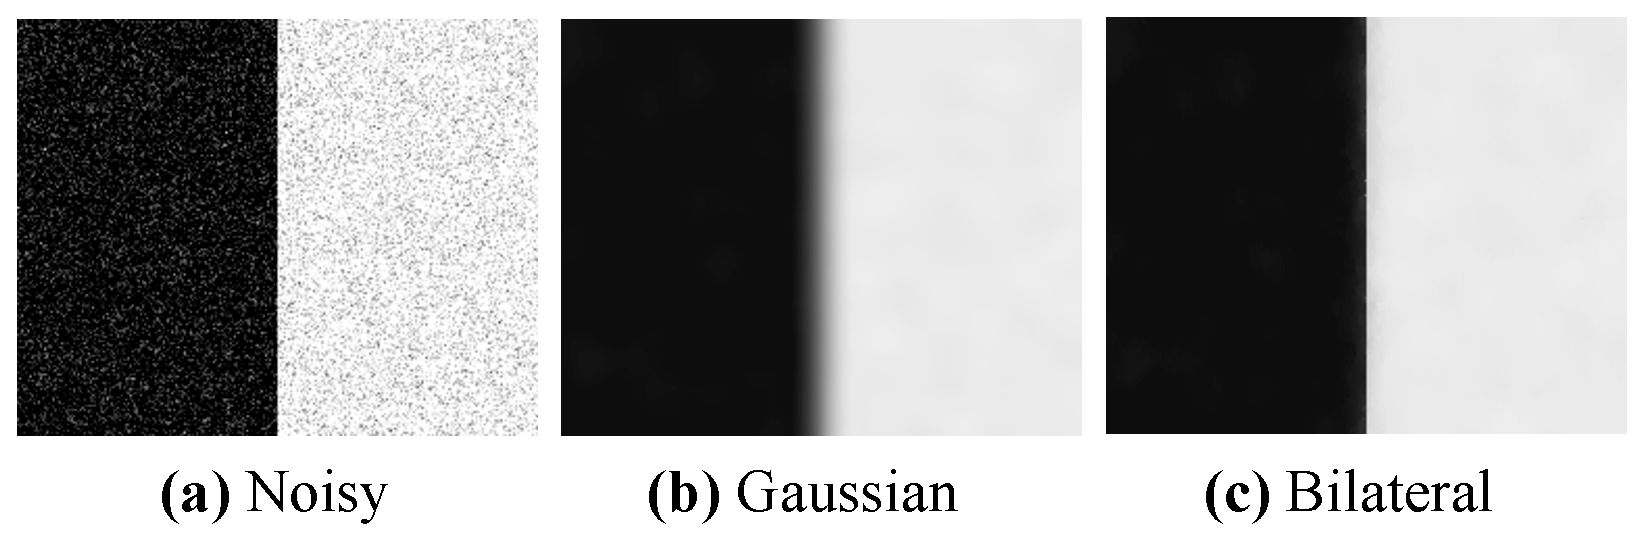
\includegraphics[width=0.65\textwidth]{figures/pt/gaussian-and-bilateral-filters}
	\caption{双面过滤器同时考虑空间和颜色距离,使得过滤后的图像能够很好的保留物体的边缘特征,而传统的高斯过滤器则仅考虑空间距离,边缘部分过于模糊,导致较大的偏差}
	\label{f:pt-gaussian-and-bilateral-filters}
\end{figure}

在图像处理(image processing)\myindex{图像处理}{image processing}领域,其中一种常用且简单的过滤器称为双边过滤器(bilateral filter)\cite{a:Bilateralfilteringforgrayandcolorimages,a:Ontheoriginofthebilateralfilterandwaystoimproveit},双边过滤器是一种能够有效识别图像中颜色边缘区域的过滤器,它将一些传统的过滤器(如高斯过滤器)同时作用到空间和颜色范围,其过滤权重系数形式如下:

\begin{equation}
	w_{bf}(p,q)=\text{exp}\Biggl(  \cfrac{-||p-q||^{2}}{2\sigma^{2}_{s}}\Biggl)\text{exp}\Biggl(  \cfrac{-||c_p-c_q||^{2}}{2\sigma^{2}_{r}}\Biggl)
\end{equation}

\noindent 这里$c_p$和$c_q$分别表示$p$和$q$点的颜色值,$\sigma^{2}_s$和$\sigma^{2}_r$是用来调节图像和颜色空间距离的参数,它们其实就是高斯曲线的方差。例如,当两个采样之间的空间距离或者颜色差异越大时,上述的权重系数就会越小,对颜色空间的过滤使得过滤器可以很好地识别图像的颜色边缘特征,如图\ref{f:pt-gaussian-and-bilateral-filters}(c)所示。

然而双边过滤器的一个问题是,由于颜色范围的距离计算直接引入了采样样本,这些样本本身是带有噪点(方差)的,所以其权重也受到了噪点的影响。为了降低颜色采样噪点对过滤权重的影响,一些方法\cite{a:AnovelMonteCarlonoisereductionoperator}通过首先对颜色空间使用一个低通过滤器以减少方差,然后再使用上述的公式进行计算,这里要讨论的是另一种称为非局部均值过滤器\cite{a:Areviewofimagedenoisingalgorithmswithanewone}的方法,它通过计算每个像素周围一定范围领域内(而不是单个)像素颜色距离的平均值来降低噪点的影响。

\begin{figure}
	\sidecaption
	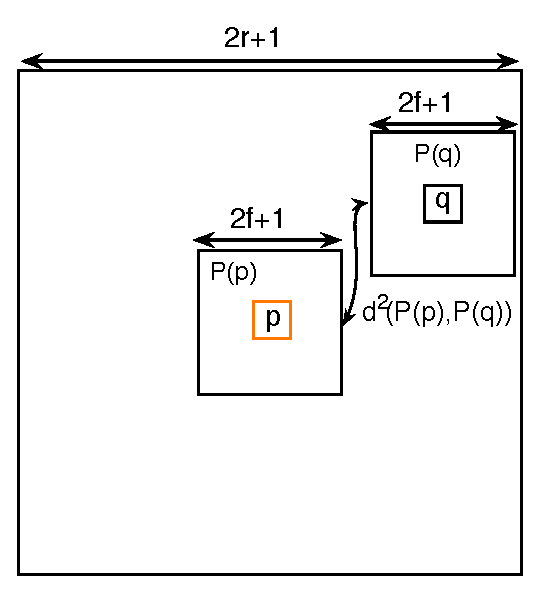
\includegraphics[width=0.45\textwidth]{figures/pt/nl-means}
	\caption{为了降低颜色采样的噪点对过滤权重计算的影响,非局部均值过滤器通过计算每个像素周围很小的一个领域块内像素的颜色距离的平均值来计算颜色距离}
	\label{f:pt-nl-means}
\end{figure}

非局部均值过滤器(non-local means filter, NL-Means)\myindex{non-local means filter}是双边过滤器的一般化,但是它计算的是围绕一个像素周围一个很小的块内部像素颜色之间距离的平均值,如图\ref{f:pt-nl-means}所示,非局部均值过滤器的权重计算公式如下:

\begin{equation}
	w_{nlm}(p,q)=\text{exp}\Biggl(  \cfrac{-||p-q||^{2}}{2\sigma^{2}_{s}}\Biggl)\text{exp}\Biggl(  \cfrac{-||\mathcal{P}_p-\mathcal{P}_q||^{2}}{k^22\sigma^{2}_{r}}\Biggl)
\end{equation}

\noindent 这里$k$是一个用来控制过滤强度的参数,其中基于块的颜色距离的平方定义为:

\begin{equation}
	||\mathcal{P}_p-\mathcal{P}_q||^{2}=\max\Biggl( 0,  \cfrac{1}{|\mathcal{P}|}\sum_{n\in\mathcal{P}_0} d(p+n,q+n)\Biggl)
\end{equation}

\noindent 其中,$\mathcal{P}_p$表示一个以$p$为中心的尺寸为$|\mathcal{P}|$(通常为$7\times 7$)的正方形块,$\mathcal{P}_0$表示块内各个相对于中心像素的偏移。这里的范围距离函数$d(p,q)$表示相应两个颜色之间的差异的平方,即:$d(p,q)=||c_p-c_q||^{2}$。

由此可以看出,与一般高斯过滤器仅考虑空间距离不同,非均值过滤器考察的是周围相邻像素颜色的相似性,每个像素与周围像素在进行比较和计算时,其实是比较它们周围一定区域内像素值的相似性,并以此相似性来决定混合权重值。因此参与过滤的周围像素值可能来自一个很大的范围,这就是非局部(non-local)的来源。




\paragraph{减小颜色采样噪点导致的偏差}
跟单纯计算空间距离的高斯过滤器不同,双边和非局部均值过滤器由于引入了颜色空间,而颜色是路径采样的结果,它们本身包含噪点,所以其参与计算的过滤器也会受到噪点的影响,导致颜色空间距离平方的估计是有偏的,其会造成对真实距离的平方值的过度估计。

为了消除过滤器与颜色样本的相关性导致的偏差,\cite{a:Areviewofimagedenoisingalgorithmswithanewone}提出了一种简单的方法,他们假设颜色样本是均匀分布的,所以可以通过直接减去两个像素的方差来实现:

\begin{equation}\label{e:pt-buades}
	d(p,q)=||c_p-c_q||^{2}-2\sigma^{2}_r
\end{equation}

\noindent 然而,蒙特卡洛估计通常导致不均匀的噪点分布,这些噪点的类型和幅度随着场景的几何复杂度,物体材质,光照传输,透镜效果等而变化。\cite{a:AdaptiveRenderingwithNonLocalMeansFiltering}在此基础上提出了一种改进方法:

\begin{equation}
	d(p,q)= \cfrac{||c_p-c_q||^{2}-(Var_p+Var_{p,q})}{ \cfrac{\epsilon+Var_p+Var_q}{2\sigma^{2}_r}}
\end{equation}

\noindent 这里$Var_p$表示$p$点的方差,它是一个过滤器过滤范围内所有样本计算出来的方差\footnote{非局部均值过滤器的过滤范围是由参数$r$决定的。},$Var_{p,q}=\min (Var_p,Var_q)$用于将$q$点的方差限制到最大值为$p$的方差,这可以防止附近光照强度更强的区域形成的更大的方差不会消除掉颜色距离的影响(毕竟颜色距离才是计算权重系数的重要依据),$\epsilon$是一个用于防止分母为0的一个很小的偏移。可以看出,当$Var_p=Var_q=\sigma^{2}$时,上式和式\ref{e:pt-buades}是等效的。

那么剩下的问题就是怎样估算过滤像素的均方差用于选择过滤范围。双边或者非局部均值过滤器由于引入了颜色样本,其过滤权重计算被引入偏差,为了考虑颜色样本噪点带来的影响,\cite{a:AdaptiveRenderingwithNonLocalMeansFiltering}创新性地引入了双缓冲过滤的技术用于解决很多由于颜色相关性带来的问题。






\paragraph{双缓存过滤}
由于引入了颜色值的计算,非局部均值过滤器的权重值是和其原始输入信号相关的,即它会受到噪点的影响,而后续与之过滤相关的计算(例如后面即将讨论的过滤后图像的误差估计)过程也会受到这种相关性的影响。为此,\cite{a:AdaptiveRenderingwithNonLocalMeansFiltering}引入了双缓存过滤技术用来解决这个问题。

输入信号虽然是有噪点的,但是这些样本本身是相互独立的。因此如果我们在每次迭代中将这些输入样本平均分成A和B两个图像缓存,它们分别用各自的样本计算出一组过滤器,然后对这些样本进行交叉过滤(cross filtering)\myindex{叉过滤}{cross filtering}:即用缓存A/B计算出的过滤器其对缓存B/A中对应位置的像素进行过滤,这样过滤器就与像素样本之间是独立的,因为该过滤器并不是通过使用参与过滤的那些颜色的值计算出来的(正如前面非局部均值过滤器的计算那样),这种技术称为双缓存过滤(dual-buffer filtering)\myindex{双缓存过滤}{dual-buffer filtering}。接下来我们将讨论双缓存过滤怎样被用来解决由于非局部均值过滤器引入颜色样本带来的相关性问题(过滤的过程保留的颜色样本噪点)。





\paragraph{过滤范围选择}
现在我们已经知道了非局部均值过滤器的表述形式(过滤权重系数公式),接下来我们要计算该过滤器作用于每个像素之后的均方差,进而用于指导选择适当范围的过滤器。

由于非局部均值过滤器考虑了颜色之间的距离,因为它比单纯考虑空间距离的高斯过滤器要好得多,例如在实践中,设置$k=0.5$几乎能够很好地作用于大部分场景而不需要选择过滤的范围,但是有时候更大范围的过滤器是更可取的,所以\cite{a:NonlinearlyWeightedFirstorderRegressionforDenoisingMonteCarloRenderings}选择在$k=\{0.5,1.0\}$之间执行过滤范围选择。

在后面的内容中,我们将介绍一些直接估算均方差的方法,例如SURE\cite{a:SUREbasedOptimizationforAdaptiveSamplingandReconstruction}能够直接对一个非线性过滤器进行均方差估计,但是它要求计算过滤器的导数;\cite{a:AdaptiveRenderingbasedonWeightedLocalRegression}能够直接估算方差和偏差,但是它假设过滤器的权重系数是没有噪点(noise-free)的,因此也不适用于非局部均值过滤器。因此,\cite{a:NonlinearlyWeightedFirstorderRegressionforDenoisingMonteCarloRenderings}提出一种利用前面的双缓存过滤机制的更一般的估算均方差的方法。

考虑过滤后像素的值$F$和输入的带噪点的值$C$之间距离的平方,再减去$C$的方差(这和前面消除噪点与过滤器相关性的原理类似),上述表达式的期望为:

\begin{equation}
	E[(C-F)^{2}-Var_C]=Bias^{2}_F+Var_F-2Cov_{C,F}
\end{equation}

\noindent 如果输入和过滤后的结果之间的无关的,则上式可以被用作对均方差的一个无偏估计。这对于非局部均值过滤器显然是不适应的,因为用于过滤的权重系数是和样本之间相关的,因此过滤的结果也是和样本相关的,但是这个问题却可以通过前面的双缓存过滤来解决。因此,使用前面讨论的交叉过滤,得到两个缓存的均方差估计:

\begin{equation}
	\begin{aligned}
		MSE_{F_1}=&(F_1-C_2)^{2}-Var_{C_2}\\
		MSE_{F_2}=&(F_2-C_1)^{2}-Var_{C_1}
	\end{aligned}
\end{equation}

\noindent 这里$Var_{C_1}=Var_{C_2}=2Var_C$,$Var_C$是所有两个缓存中样本的方差。在分别对两个缓存的均方差进行估计后,通过计算两个缓存的平均值来获得最终均方差,即:$F=(F_1+F_2)/2$。在这个合并的过程中,$F$的偏差是保持不变的,但是它们的方差减半了,所以最终的均方差估计为:

\begin{equation}
	MSE_F= \cfrac{MSE_{F_1}+MSE_{F_2}}{2}-Var_F
\end{equation}

\noindent 上述的估计是无偏的,因为两个缓存之间是相互独立的。虽然交叉过滤会引入一些相关性,但是实践中这个相关性很小。在对过滤器进行均方差估计之后,就可以按照前面的框架进行过滤范围的选择。







\subsubsection{过滤权重计算加入特征信息}\label{sec:pt-feature-filtering}
虽然样本颜色值能够有效识别图像的一些细节,但由于它本身含有较高噪点,因此单纯依靠颜色值的过滤是低效的;另一方面,像素的一些其他信息,例如法线,纹理,深度等,这些信息和渲染的图像是高度相关和低噪的\footnote{尽管特征信息相对于颜色值的噪点更小,在本节将看到它们仍然需要进行去噪处理。},这些信息能够更容易地区分图像的一些(如边缘等)特征,我们称这些每像素(per pixel)信息为特征缓存(feature buffers)\myindex{特征缓存}{feature buffers}或者辅助缓存(auxiliary buffers)\myindex{或者辅助缓存}{auxiliary buffers}。

特征信息通常是通过直接发射摄像机光线,然后对每个像素内的样本求平均值得到,这也是其噪点较少的原因\footnote{由此也可以看出,特征信息通常不能有效地分辨间接光阴影,焦散等涉及多次反射效果。},但是正如\cite{a:OnFilteringtheNoisefromtheRandomParametersinMonteCarloRendering}所分析,特征信息在一些特殊的效果(如聚焦)下也含有一定的噪点需要消除。特征缓存虽然高效,但是在该特征信息没有覆盖的区域(或者说特征信息与颜色信息相关度很低时),图像的过滤会导致过度模糊,因此,一些新的基于组合颜色值和特征缓存的过滤器被提出,它们根据图像分布在图像细节(颜色值)和特征信息之间取得平衡,本节我们就将讨论其中的一些解决方案和其思路。

在每个迭代的路径采样后,如果有额外的每像素特征信息可用,同颜色值一样,我们可以将特征信息加入到前面的双向或非局部均值过滤器权重计算当中,用来增强过滤的品质,这称为联合过滤(joint filtering)\myindex{联合过滤}{joint filtering},例如:

\begin{equation}
	\begin{aligned}
		w_{jbf}(p,q)=&w_{bf}(p,q)w_{aux}(p,q)\\
		w_{jnlm}(p,q)=&w_{nlm}(p,q)w_{aux}(p,q)
	\end{aligned}
\end{equation}

\noindent 这里$w_{aux}(p,q)$表示额外特征缓存的权重系数,给定$k$个特征缓存,$\mathbf{f}=(f_1,\cdots,f_k)$,该特征缓存的权重系数计算如下:

\begin{equation}
	w_{aux}(p,q)=\prod^{k}_{i=1}exp(-d_{f,i}(p,q))
\end{equation}

\noindent 这里:

\begin{equation}\label{e:pt-feature-distance}
	d_{f,i}(p,q)= \cfrac{||f_{i,p}-f_{i,q}||^{2}}{2\sigma^{2}_{i,p}}
\end{equation}

\noindent 由于特征缓存的噪点较小,所以通常直接使用双向过滤即可,不必使用如上面讨论的针对颜色值的非局部均值过滤。

尽管特征信息的引入,在权重计算的形式上看起来并不太复杂,然而它也引入了新的问题。首先,特征缓存也是具有噪点的,这需要适当的方法进行控制;怎样估算新的联合过滤器的误差,以及怎样在特征信息描述的底噪信息和颜色值描述的图像颜色细节之间进行平衡。本节后面我们首先讨论这些问题,在第\ref{sec:pt-first-order-regression}节则会讨论怎样利用特征信息用来进行更精确的局部多项式回归。







\paragraph{特征缓存的降噪处理}
\cite{a:OnFilteringtheNoisefromtheRandomParametersinMonteCarloRendering}指出,当处理如景深和运动模糊等效果时,这些特征缓存也有可能因为蒙特卡洛采样而引入噪点,因此其参与计算的权重系数也会使过滤后的图像误差更大。在那里,他们通过计算场景特征信息和蒙特卡洛随机数参数之间的依赖性(dependency),以及对高度依赖于随机数参数的特征样本设置更小的权重系数来解决这个问题。直观上,这其实仍然是在区分前面讨论的特征信息对图像细节的敏感性,例如在纹理边界或物体边缘部分,特征信息对蒙特卡洛随机数的依赖性更小,而在一些低频的区域(例如处于景深外和高度运动模糊的区域),特征信息会更容易受到随机数噪点的影响。然后\cite{a:OnFilteringtheNoisefromtheRandomParametersinMonteCarloRendering}的方法是在样本级别进行计算的,因此计算性能和内存占用都很高。

\cite{a:SUREbasedOptimizationforAdaptiveSamplingandReconstruction}提出了另一种近似方法,它将像素$p$和$q$之间的距离(式\ref{e:pt-feature-distance})除以两个像素内特征样本的方差,如下式:

\begin{equation}
	||f_{i,p}-f_{i,q}||=\sqrt{ \cfrac{||\bar{f}_{i,p}-\bar{f}_{i,q}||^{2}}{\sigma^{2}_{ip}+\sigma^{2}_{iq}}}
\end{equation}

\noindent 这里$\bar{f}$表示一个像素内多个特征样本的平均值,$\sigma^{2}_{ip}$和$\sigma^{2}_{iq}$分别表示像素$p$和$q$内对应特征样本的方差。直观上看,如果像素处于景深外或高度运动模糊区域,则这些像素的方差就会很大,所以权重系数就会减小,而颜色(或者位置)的权重会增加。这本质上和上述的思路是一致的,也是在减少颜色采样噪点大的区域内特征像素引入的权重系数。

与上述方法不同的是,考虑到特征缓存的噪点通常是较小的,即含有很小的方差,它可以很好地被过滤掉,因此\cite{a:RobustDenoisingusingFeatureandColorInformation}提出对特征缓存进行预过滤(prefiltering)。这里他们使用前面讨论的非局部均值过滤器对特征缓存进行过滤,其中对所有特征缓存使用的非局部均值过滤器的参数为$r=5$,$f=3$以及$k_c=1.0$。这样过滤的特征缓存将含有更少的噪点,然后再被用于过滤权重的计算,其预过滤计算的结果与未过滤的结果对比如图\ref{f:pt-prefiltering}所示。

\begin{figure}
	\sidecaption
	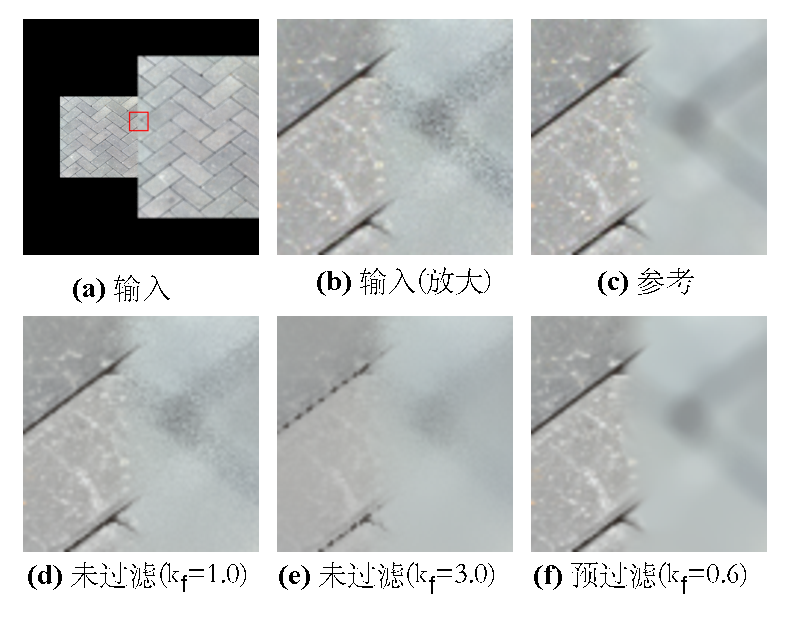
\includegraphics[width=0.65\textwidth]{figures/pt/prefiltering}
	\caption{(a)为一带有景深效果的场景,(b)为其景深交界处的放大图,(c)为参考图,图中左半部分处于焦点内,噪点较少,右半部分则处于焦点外,噪点较多;当未使用预过滤时,如果特征缓存使用的双向过滤器的过滤范围$k_f$过小(d),左边焦点内的细节被保留,但是右边焦点外的噪点很多,而过大的范围(e)又使得焦点内的图像细节丢失,(f)显示使用非局部均值预过滤的几何特征缓存能够有效消除处于景深外的噪点(图片来自\cite{a:RobustDenoisingusingFeatureandColorInformation})}
	\label{f:pt-prefiltering}
\end{figure}

由上面的内容可以看出,引入特征缓存的权重计算很重要的一点就是需要仔细分辨图像中各个局部区域内特征信息和颜色信息之间的相关性,因为特征信息一般只针对少数高频区域非常相关,而对于很多低频区域则包含更多噪点,此时颜色信息则能辨别更多图像细节。






\paragraph{范围选择}
上述的讨论使得在给定过滤范围的情况下,对特征缓存与颜色信息相关性的分析会使得权重系数的计算能够适应这种相关性,然而我们仍然需要去决定这些特征缓存使用的双向过滤器的过滤范围大小,这是一个非常棘手的问题。

前面讨论的非局部均值过滤器只包含一个参数,然而高维的特征缓存的带宽选择问题会更加复杂,并且更容易带来误差。\cite{a:RobustDenoisingusingFeatureandColorInformation}通过对所有特征信息使用相同的过滤范围,并选择过滤范围最小的一个来作为整个特征缓存的过滤范围,这样保留了特征缓存的精细部分,也避免了高维范围选择的复杂性,他们同时还更进一步地根据特征信息对图像细节的敏感度来将组合过滤器划分成三个类别:对图像细节敏感,对特征信息敏感以及两者适中,然后通过对三个类别的加权计算来更好地区分特征信息和图像信息的相关性。

关于特征缓存范围的选择,这里不会详细讨论,因为在近几年的工业中,特征缓存并不仅仅是作为一个普通额外的信息被简单地联合进权重系数的计算当中,而是将这些特征信息用来作为更精确的局部多项式回归的预测参数,这是我们接下来将要讨论的内容。






\subsubsection{局部多项式回归}\label{sec:pt-first-order-regression}
本书到目前为止,讨论了很多关于过滤(filtering)\mathindex{过滤}{filtering}的理论和运用,在第1章我们介绍它是一种根据已有离散采样进行函数重建(还原)的方法,在本章我们进一步说明过滤是一种减少随机数方差的方法,然而这些解释都没有触及过滤的数学本质,即过滤是一种关于回归分析的数学方法。

本节我们首先梳理一下回归理论的一些概念,然后介绍怎样使用回归理论来对路径采样进行更精确地适应性过滤。







\paragraph{回归分析理论基础}
回归分析(regression analysis)\mathindex{回归分析}{regression analysis}通常是指用一个或几个预测变量\footnote{或称为自变量。}(predictor variable)\mathindex{预测变量}{predictor variable}$\mathbf{x}$的函数形式来描绘响应变量\footnote{或称为因变量。}(response variable)\mathindex{因变量}{response variable}$y$平均值的统计方法。设$y$基于预测变量$\mathbf{x}$的条件均值记为$f(\mathbf{x})$,称为回归函数(regression function)\mathindex{回归函数}{regression function},回归的主要目标就是通过样本来估计总体回归函数$f(\mathbf{x})$。

一个一般的回归模型如下:

\begin{equation}
	y\approx f(\mathbf{x},\beta)
\end{equation}

\noindent 这里$y$为已知输入样本,$f$为未知的回归函数,为了进行回归分析,回归函数$f$的形式必须预先给出,它是用预测变量和参数$\beta$表述的一个函数形式,$\beta$可以根据一些已知的,不依赖于当前样本的$y$与$\mathbf{x}$之间的关系得出,上述的回归模型称为参数回归(parametric regression)。例如,假设因变量和预测变量之间存在线性关系,对于预测变量$\mathbf{x}$,有:

\begin{equation}
	f(\mathbf{x})=\alpha+\beta \mathbf{x}
\end{equation}

\noindent 或者,等效地:

\begin{equation}
	y=\alpha+\beta \mathbf{x}+\epsilon
\end{equation}

\noindent 这里方程中的误差项$\epsilon$的均值为0。具有一个预测变量的线性回归模型的示例如图\ref{f:pt-linear-regression}所示。在这一整套假设满足的条件下就得到我们常用的线性最小二乘法回归,即它使得每个预测变量$\mathbf{x}$处回归函数值与输入样本值的差(残差)的平方最小。

\begin{figure}
	\sidecaption
	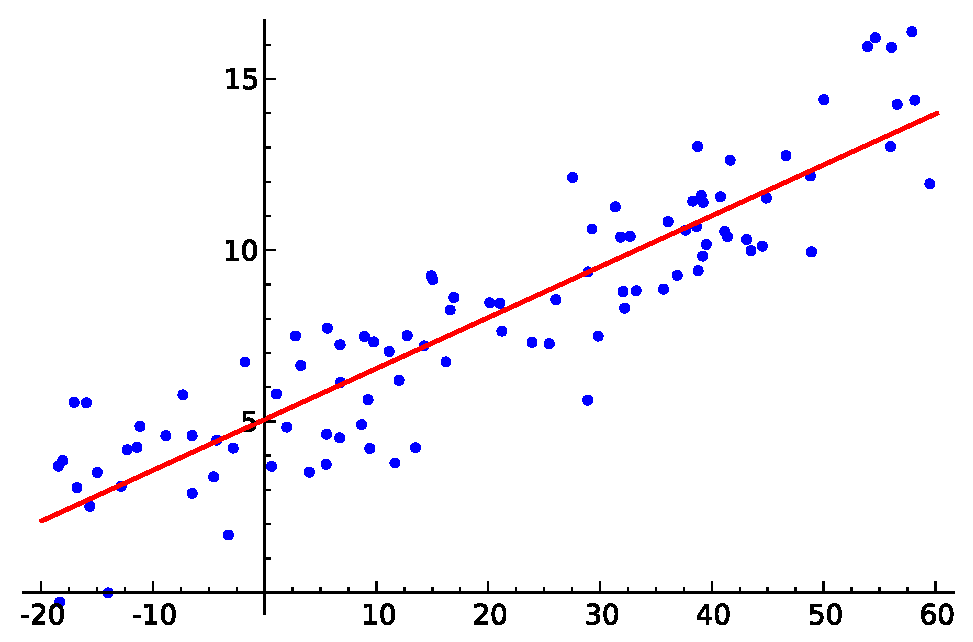
\includegraphics[width=0.65\textwidth]{figures/pt/linear-regression}
	\caption{一个简单的线性回归分析,这里只有一个独立的预测变量,其回归函数与预测变量之间呈线性关系,红色的回归函数使用最小二乘法回归得出(图片来自Wikipedia)}
	\label{f:pt-linear-regression}
\end{figure}

参数回归的回归函数仅由一些参数表达,形式通常比较简单明确,并且当模型的参数假设成立时,统计推断的精度较高,使用较少的样本就能比较准确地进行推断。然而,参会回归要求回归函数的形式必须是预先假定的,参数模型限制较多,它通常要求样本满足某种分布要求,并且模型的泛华能力较弱,当模型假设不成立时,拟合效果很差,需要修正或者更换模型。

非参数回归(nonparametric regression)\mathindex{非参数回归}{nonparametric regression}则弱化了这种假设限定,它不要求任何预定的回归函数形式,对数据的分布一般也不做任何要求,适应能力很强,并且模型的精度较高。非参数回归模型完全由样本数据驱动,因此也常称作散点图平滑(scatterplot smoothing)\mathindex{散点图平滑}{scatterplot smoothing},因为在典型的应用中,这一方法会在$y$关于$x$的散点图上绘出一条经过若干点的平滑曲线。

非参数回归方法中仅有单一的响应变量$y$和单一的预测变量$\mathbf{x}$(它不再包含任何描述回归函数形式的参数,回归函数的形式则唯一由样本数据推导而出,因此相对于参数回归,非参数回归的精确度往往依赖于大量的样本值),即:

\begin{equation}
	y=f(\mathbf{x})+\epsilon
\end{equation}

最简单的非参数回归方法是装箱法\cite{b:nonparametricregression}(Binning)\mathindex{装箱法}{Binning},它假设回归函数是一个离散函数,然后使用每个离散区间或者说箱(bins)内样本的平均值来近似回归函数。当箱很窄时,箱均值能够很好地估计回归函数。

非参数回归的进一步演化则是局部平均化(local averaging)\mathindex{局部平均化}{local averaging}。局部平均化的基本观点是,只要回归函数足够平滑,$x$取值位于焦点$x_0$附近的观测就会给$f(x_0)$提供丰富的信息。局部平均化与装箱法很相似,只是我们不再把数据切割为互相不重合的箱,而是通过在数据上连续移动一个箱(或者称为一个窗体)来计算进入窗体中观测的平均值,这个窗体(window)\myindex{窗体}{window}其实就是过滤使用的范围。我们可以以焦点值$x_0$为中心建立固定宽度为$w$的窗体,或者我们可以调整窗体的宽度使其能够固定容纳$m$个观测样本,这些观测样本称为焦点值的$m$个最近邻。

在估计$f(x_0)$的时候,一种可取的方法是给予接近焦点$x_0$的观测样本更高的权重,同时给予远离焦点的观测样本更低的权重。令$z_i=(x_i-x_0)/h$表示标尺化后第$i$个观测样本的$x$值与焦点$x_0$之间有符号的距离,标尺因子$h$--它被看做估计值的带宽(bandwidth)\myindex{带宽}{bandwidth},扮演了窗体宽度之于局部平均数的角色。这样的估计回归函数估计方法称为核估计(kernel estimate)\mathindex{核估计}{kernel estimate},它是一种局部加权平均化(local-weighted averaging)\mathindex{局部加权平均化}{local-weighted averaging},是局部平均化的一个扩展。

在核估计中,我们需要一个核函数$K(z)$来将最大的权重值赋予靠近焦点$x_0$的样本,然后随着$|z|$的增长令权重对称地平滑下降。只要能满足这一特征,究竟选择哪一种核函数并不十分重要。得到权重$w_i=K[(x_i-x_0)/h]$后,我们可以进一步通过加权局部平均化计算出$x_0$处的拟合值。常见的核函数如高斯(正态)核,三次方核以及矩形核等。相比局部平均化回归,核估计显得更加平滑,如前所述,核估计量不同的带宽能够被用来控制估计回归函数的平滑程度,较大的带宽带来更平滑的结果。

至此,我们将前面讨论的过滤与其数学本质联系了起来,它们是用已知离散样本值来拟合回归函数的一个回归分析问题,由于图像分布非常复杂,其回归函数很难进行参数化,因此它属于非参数回归方法,使用局部平滑的方式用局部区域的样本值来估算(加权平均)焦点位置的回归值。

然而,到目前为止,本节讨论的过滤都是假设回归函数焦点处的值是一个常数,为表述方便,我们这里将相关的符号针对图像作出调整:用$c_p$表示图像回归中的输入预测样本值,$\hat{c}_p$为回归函数在焦点$p$处的值,那么使用最小二乘法拟合(使加权残差平方和最小)回归函数,得:

\begin{equation}
	\hat{c}_p=\underset{\hat{c}_p}{\text{arg min}}\sum_{q\in\mathcal{N}_p}(c_q-\hat{c}_p)^{2}\tilde{w}_\mathbf{x}(p,q)
\end{equation}

\noindent 上述(节本节前面讨论的过滤技术)的回归可以称之为是零阶回归(zero-order regression)\mathindex{零阶回归}{zero-order regression}因为它们把局部领域的像素值当做一个常数来拟合回归函数,它仅考虑两个像素之间的颜色差异,而忽视了像素之间的变化特征(如梯度)。更精确的预测模型是使用多项式,它将核估计扩展为焦点$x_0$处使用核权数$w_i=K[(x_i-x_0)/h]$的多项式拟合,这样的回归方法称为局部多项式回归(local polynomial regression)\mathindex{局部多项式回归}{local polynomial regression},例如预测变量$x$的$n$阶多项式为:

\begin{equation}
	y=\alpha+\beta_1 x+\beta_2 x^{2}+\cdots+\beta_p x^{n}+\epsilon
\end{equation}

\noindent 当$n=1$时对应线性拟合,当$n=2$时对应二次函数拟合,以此类推。对常数项(即均值)的拟合则对应$n=0$。例如,针对图像使用最小二乘法拟合的的一阶回归(first-order regression)\mathindex{一阶回归}{first-order regression}公式为:

\begin{equation}\label{e:pt-first-order-regression}
	[\hat{c}_p,\nabla\hat{c}_p]=\underset{\hat{c}_p,\nabla\hat{c}_p}{\text{arg min}}\sum_{q\in\mathcal{N}_p}(c_q-\hat{c}_p-\nabla\hat{c}_p\cdot (\mathbf{y}_q-\mathbf{y}_p))^{2}\tilde{w}_\mathbf{x}(p,q)
\end{equation}

\noindent 这里$\mathbf{y}$和$\mathbf{x}$一样,是预测变量矢量。需要注意的是,一般情况下$\mathbf{y}=\mathbf{x}$,但并不总是这样,即我们可以使用预测变量不同的维度来计算过滤权重系数,而使用另一些维度来进行回归计算。

局部多项式回归引入了预测变量和响应变量之间的相关性,因而能够更精确地进行回归函数的估计。下面,我们就将讨论多项式回归怎样被运用于前面讨论的适应性过滤中,这也是目前工业中比较主流的方法。更多关于局部回归的知识,可以参阅\cite{b:LocalRegressionandLikelihood, b:nonparametricregression,a:SmoothingbyLocalRegression:PrinciplesandMethods}等。







\paragraph{局部回归在适应性过滤中的运用}
在图像空间的降噪技术领域,\cite{a:AdaptiveRenderingbasedonWeightedLocalRegression}比较早地引入局部回归方法用于图像重建,根据上面的内容,局部回归(local regression)\mathindex{局部回归}{local regression}是一种基于焦点$\mathbf{x}$一定领域内的样本输入用来拟合曲线或者曲面$f(\mathbf{x})$的一种平滑方法:

\begin{equation}
	y=f(\mathbf{x})+\epsilon
\end{equation}

\noindent 在本节讨论的图像过滤问题中,这里$y\in\mathbb{R}^{1}$是表示响应变量的一个标量,它表示蒙特卡洛采样输出的(即过滤阶段输入的)带噪点的图像;而$f(\mathbf{x})\in\mathbb{R}^{1}$表示要拟合的回归函数,其值仍为标量\footnote{注意,这里是分别对图像颜色值的三个通道进行拟合,所以以下不再单独说明每个通道。};$\mathbf{x}\in\mathbb{R}^{D}$是一个$D$维的特征矢量,它包括像素的位置,以及其他任何特征信息,如纹理,深度,法线等。

根据一阶泰勒多项式,以特征向量$\mathbf{x}^{c}$为焦点,邻近$\mathbf{x}$处的未知的拟合函数值$f(\mathbf{x})$可表示为:

\begin{equation}
	f(\mathbf{x})\approx f(\mathbf{x}^{c})+\nabla f(\mathbf{x}^{c})^{T}(\mathbf{x}-\mathbf{x}^{c})
\end{equation}

\noindent 因此,根据前面讨论的局部多项式回归,上式表述的回归函数可以使用式\ref{e:pt-first-order-regression}表示的最小二乘法一阶回归方程计算而出。在这里,使用最小二乘法可以求出回归函数在$p$点处的值$\hat{c}_p$,以及在$p$点处的梯度$\nabla \hat{c}_p$,剩下的重要的事情是对过滤器$\tilde{x}_x(p,q)$执行范围选择。

\cite{a:AdaptiveRenderingbasedonWeightedLocalRegression}通过在高维下计算各种类型的特征缓存的过滤范围来计算使得估计的均方差最小化,虽然精度较高,但是计算成本很高;\cite{a:AdaptiveRenderingwithLinearPredictions}在此基础上通过仅计算一些稀疏的像素来进行近似优化;\cite{a:AdaptivePolynomialRendering}则采用一种完全不同与过滤带宽选择的策略,它通过适应性地选择多相似的阶数来适应图像信号的特征,例如他们在高曲率的区域使用更高阶数的多项式来进行重建,在一些比较平滑的区域则选择低阶数的多项式;本节,我们则仅讨论\cite{a:NonlinearlyWeightedFirstorderRegressionforDenoisingMonteCarloRenderings}中使用的效率更高的方法,但是通过这种方法讨论,我们仍然能够明白局部回归方法的思路。

在时\ref{e:pt-first-order-regression}表示的一阶回归模型中,特征缓存梯度信息的引入大大提升了回归函数的精确度,然而高维的特征矢量却使得带宽选择的计算成本非常高。考虑到特征信息已经通过在一阶回归多项式中提升了回归函数的精确度,\cite{a:NonlinearlyWeightedFirstorderRegressionforDenoisingMonteCarloRenderings}提出仅使用前面讨论的非局部均值过滤器作为式\ref{e:pt-first-order-regression}中的回归核函数(即权重系数不考虑特征缓存),这样做有两个好处:首先,当特征缓存不能提供有效信息时(例如前面讨论的景深之外的特征信息噪点较大),颜色值可以提供更多的细节;其次,这使得过滤带宽的选择和前面非局部均值过滤器的带宽选择的成本一致,即只需要一个参数,大大降低了一阶回归带宽选择的计算成本。

虽然,非局部均值过滤器由于忽视特征缓存而可能丢失很多高频的特征信息,但是\cite{a:NonlinearlyWeightedFirstorderRegressionforDenoisingMonteCarloRenderings}说明在一阶回归中,选择非局部均值过滤器也能呈现较高的图像质量。直观上理解,一阶回归模型和非局部均值过滤器之间形成互补关系,式\ref{e:pt-first-order-regression}中的一阶回归模型允许更好地探索任何特征缓存也颜色值相关的区域,而非局部均值过滤器使得在这种相关性较弱的区域更好地体现图像的颜色细节。

尽管有前面讨论的预过滤技术来减少特征缓存的方差,但是特征缓存仍然是和颜色缓存的噪点具有一定的相关性,所以在\cite{a:NonlinearlyWeightedFirstorderRegressionforDenoisingMonteCarloRenderings}中,他们使用类似前面的交叉过滤技术来进行一阶回归:即使用A缓存中的特征信息来拟合B缓存中的回归函数值,通过这样来消除颜色缓存和特征缓存中噪点的相关性。










\section{梯度域渲染}\label{sec:pt-gradient-domian-path-tracing}
路径追踪本质上是一个蒙特卡洛方法问题,蒙特卡洛估计的收敛速度决定了路径追踪技术的低效。传统的方差缩减技术(第\ref{sec:Variance-Reduction}节)仍然可以被用于路径追踪技术中,例如前面讨论的双向路径追踪技术本质上就是复合重要性采样,而根据BRDF等分布进行采样对则对应于重要性采样,同样,拟蒙特卡洛方法也被大量应用于路径追踪技术中。

由于光照传输的复杂性,这些基本的采样方法显然是不够的,我们还需要根据光照传输的特征,挖掘一些更高级的采样技术。请注意,本书大体上将所有的路径采样技术分为两类:即基础路径采样技术以及本节讨论的高级路径采样技术。基础路径采样技术包括本节讨论的非双向和双向路径采样,第\ref{chp:pm}章讨论的光子映射以及第\ref{chp:mlt}章讨论的梅特波利斯光照传输,这些技术只是路径生成的方式不同,其核心并没有太大差异,即通过相互独立的随机路径的平均值来近似图像积分。

由于相互独立的路径无法分辨图像的局部分辨特征,因此这里的高级路径采样技术主要是指能够借助路径之间的相关性来辅助进行图像局部特征辨识的技术。这包括本节要讨论梯度域渲染,以及第\ref{chp:mlt}章会介绍的半矢量空间光照传输。另外,从这个角度来看,本节前面讨论的所有和频率域相关的技术其实也属于这个范畴,本质上它也是通过研究路径的局部特征来更好地对路径进行采样和过滤。




	
\subsection{基于梯度域的图像重建}
空间微分已经被大量运用于图像编辑中,例如其中一些主要的运用包括图像锐化,边缘检测和图像重建(例如克隆,部分区域提取等)等,而后者正是本节基于梯度域路径追踪技术的基础\footnote{尽管梯度域路径追踪使用和基于梯度的图像重建相同方法,但是我们将在本节看到它们本质上是两种不同的思路:后者通常取一个图像某部分的梯度来和另一个图像进行合成,因此可以实现克隆,部分图像提取等功能,而前者是利用梯度的高频低能量特性来对路径按照频率划分进行重要性采样。},因此,了解图像编辑中空间微分的一些基本概念将有助于我们学习本节的知识。

图像处理中的一阶微分使用梯度幅值来表示的,对于图像分布函数$f(x,y)$,$f$在坐标$(x,y)$处的梯度(gradient)\myindex{梯度}{gradient}定义为二维列向量:

\begin{equation}
	\nabla f\equiv grad(f)\equiv\mathbf{g}=\begin{bmatrix}
		g_x\\ g_y
	\end{bmatrix}=\begin{bmatrix}
		 \cfrac{{\rm \partial} f}{{\rm \partial} x} \\
		 \cfrac{{\rm \partial} f}{{\rm \partial} y}
	\end{bmatrix}
\end{equation}

\noindent 该向量指出了位置$(x,y)$处$f$的最大变化率的方向,在一个2D的图像中,这个变化发生的最短距离是在两相邻像素之间,所以图像的梯度的两个分量表示为两个像素之间的差值,定义为:

\begin{equation}
	\begin{aligned}
		 \cfrac{{\rm \partial} f}{{\rm \partial} x} &=f(x+1,y)-f(x,y)\\
		 \cfrac{{\rm \partial} f}{{\rm \partial} y} &=f(x,y+1)-f(x,y)
	\end{aligned}
\end{equation}

\noindent 在图像编辑中的图像重建问题可以归结为:求一个函数$f(x,y)$,使得其梯度$\nabla f(x,y)$尽可能地接近一个给定的梯度场(gradient field)\myindex{梯度场}{gradient field}$\mathbf{g}(x,y)$,这个问题通常可以通过求解如下积分的最小值(满足最小差异)来实现:

\begin{equation}\label{e:pt-image-reconstruction}
	{\rm \iint} ||\nabla f-\mathbf{g}||^{2}dxdy
\end{equation}

\noindent 在图像编辑中,梯度场$\mathbf{g}$通常来自于另一个图像(或者其部分图像),这可以用于实现如无缝克隆等功能,如图\ref{f:pt-image-reconstruction}所示,来自不同图像的部分图像区域被无缝插入到另一个图片中。

\begin{figure}
\begin{fullwidth}
	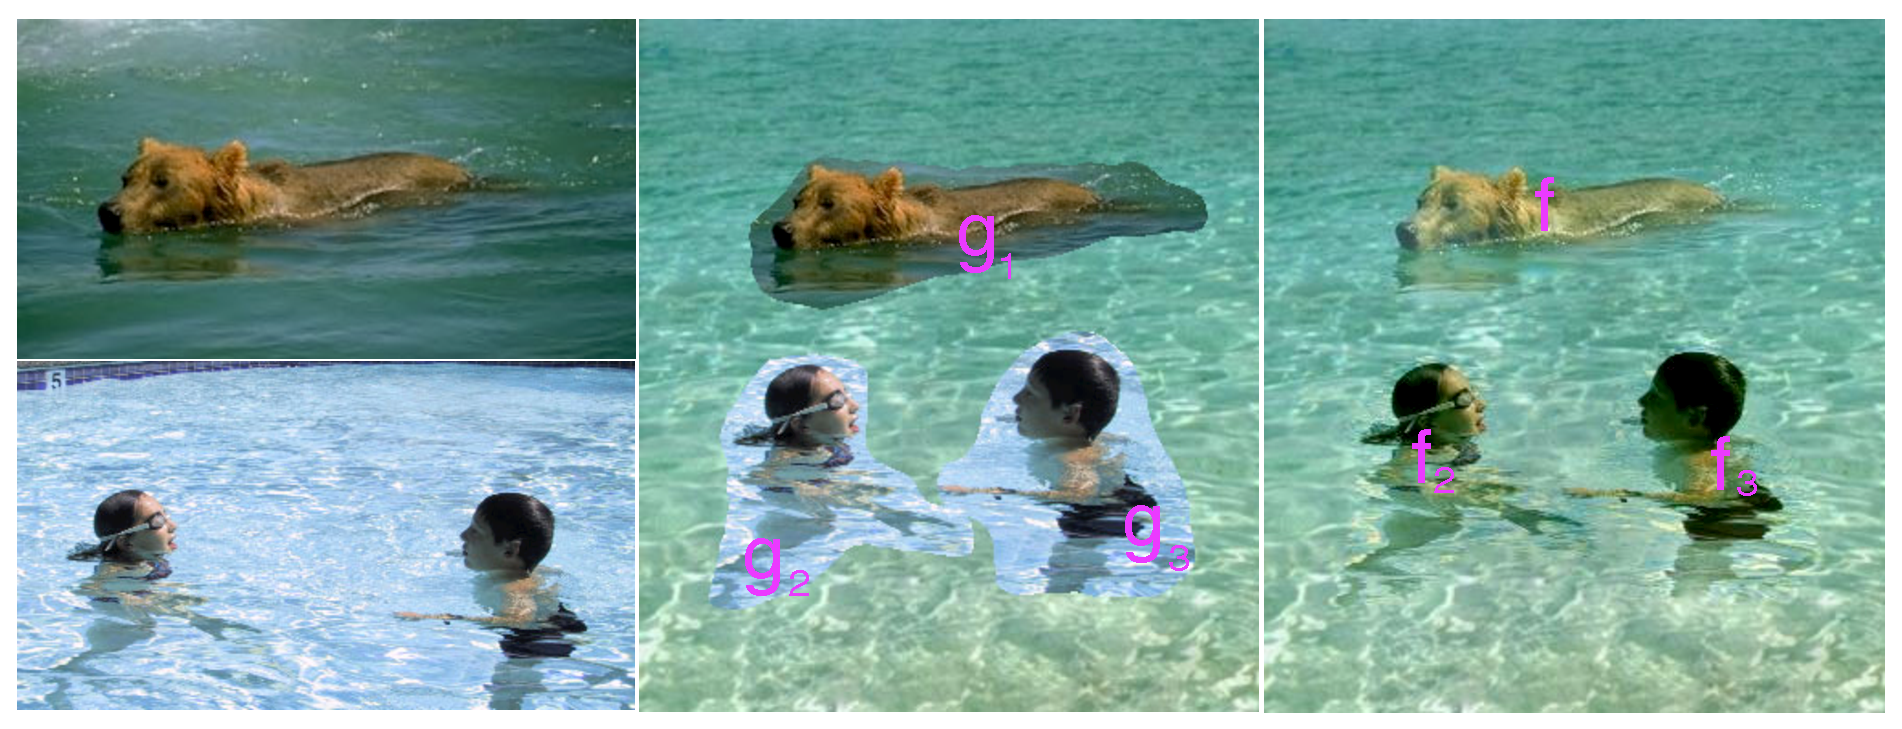
\includegraphics[width=1.0\thewidth]{figures/pt/image-reconstruction}
	\caption{在数字图像编辑中,梯度场被用于克隆,图像提取等编辑操作,图中从源图(左边上下两图)提取的梯度场($\mathbf{g}_1$,$\mathbf{g}_2$和$\mathbf{g}_3$)被用于右边的图中进行重建并计算出重建后的图像($f_1$,$f_2$和$f_3$)(图片来自\cite{a:PoissonImageEditing})}
	\label{f:pt-image-reconstruction}
\end{fullwidth}
\end{figure}

通过求解欧拉-拉格朗日方程(Euler-Lagrange equation)\myindex{欧拉-拉格朗日方程}{Euler-Lagrange equation},式\ref{e:pt-image-reconstruction}中的最优解$f$满足下述的泊松方程(Poisson equation)\myindex{泊松方程}{Poisson equation}:

\begin{equation}
	\nabla^{2}f=\nabla\cdot\mathbf{g}
\end{equation}

\noindent 这里$\nabla^{2}= \cfrac{{\rm \partial}^{2}}{{\rm \partial} x^{2}}+ \cfrac{{\rm \partial}^{2}}{{\rm \partial} y^{2}}$表示拉普拉斯算子(Laplace operator)\myindex{拉普拉斯算子}{Laplace operator},它是函数$f$的二阶偏微分,$\nabla= \cfrac{{\rm \partial}}{{\rm \partial} x}+ \cfrac{{\rm \partial}}{{\rm \partial} y}$称为梯度算子(gradient operator)\myindex{梯度算子}{gradient operator},如前所述,它是函数$f$的一阶微分。如果我们将偏微分用下标简记,则上式可以表示为:$f_{xx}+f_{yy}=g^{x}_x+g^{y}_y$(为了表述,这里将梯度矢量的分量标识移动到右上角了)。

式\ref{e:pt-image-reconstruction}直接将一个图像的梯度场插入到另一个图像中,这可能导致不正确的结果,例如图\ref{f:pt-image-reconstruction}中插入的梯度图和源图的颜色相差甚远,这是由于梯度场仅记录了图像的灰度变化,不包含任何源图的颜色信息,尽管如此,由于人眼视觉对于颜色变化比颜色本身更敏感,所以看起来不会有很大问题。

然而这引出另一个问题,即在式\ref{e:pt-image-reconstruction}的基础上增加一个供参考的数据函数$u(x,y)$,使得$f(x,y)$尽可能地接近于$u$,因此新的问题演变成求解下列方程的最小值:

\begin{equation}\label{e:screen-poisson-reconstruction}
	{\rm \iint} \alpha (f-u)^2+||\nabla f-\mathbf{g}||^2dxdy
\end{equation}

\noindent 这里$\alpha$是一个用于控制目标函数$f$在参考数据函数$u$和输入的梯度场$\mathbf{g}$之间逼真度的平衡常数。

参考\cite{a:FourierAnalysisofthe2DScreenedPoissonEquationforGradientDomainProblems},上述方程可以转换为求解下述方程:

\begin{equation}
	\alpha f-(f_{xx}+f_{yy})=\alpha u-(g^{x}_x+g^{y}_y)
\end{equation}

\noindent 或者下述的等效方程:

\begin{equation}
	\alpha f-\nabla^{2}f=\alpha u-\nabla\cdot\mathbf{g}
\end{equation}

\noindent 上述方程的左边称为筛选的泊松方程(screened Poisson equation)\myindex{筛选的泊松方程}{screened Poisson equation},通常运用于物理学中,当$\alpha=0$时,上式演变为泊松方程。

有了上述理论基础,我们就可以基于一个参考图像$u$和一个梯度场$\mathbf{g}$来重建一个图像$f$,如图\ref{sec:pt-screened-poisson-equation}所示,这就是本节梯度域路径追踪的基础。所以在梯度域路径追踪技术中,我们的目标就是要利用路径采样得到一个梯度场和一个参考图像。

\begin{figure}
	\sidecaption
	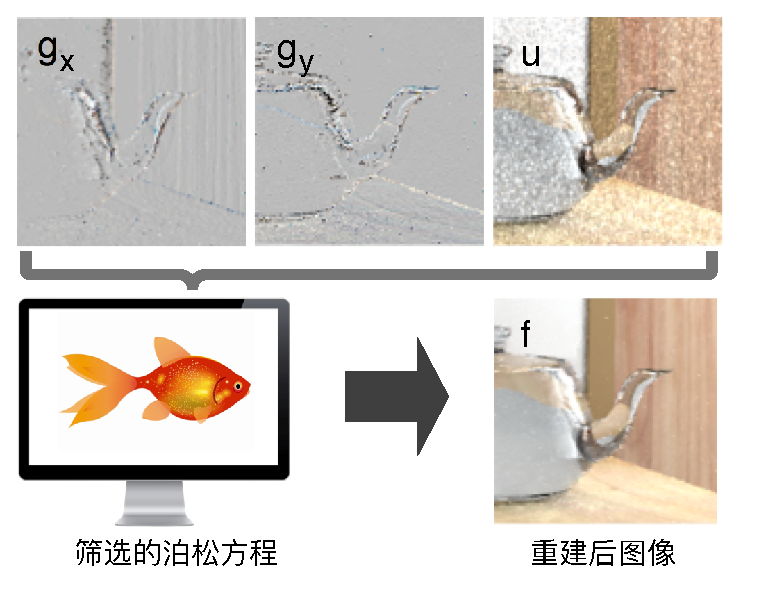
\includegraphics[width=0.55\textwidth]{figures/pt/screened-poisson-equation}
	\caption{在梯度场路径追踪技术中,最终图像可以通过一个梯度场图像和一个稀疏的参考图像来进行重建,这两个图像都是通过路径采样计算得到的,梯度场反映了图像傅里叶变换的高频部分,而稀疏参考图像对应于低频部分(图片来自\cite{a:GradientDomainPathTracing})}
	\label{sec:pt-screened-poisson-equation}
\end{figure}

然而由于这里的参考图像$u$和梯度场$\mathbf{g}$来自同一个图像$f$,所以直接对参考图像$u$使用梯度算子$\nabla$然后与$u$进行组合并没有什么意义,梯度域路径追踪技术的重点就在于梯度场和参考图像的计算方式上,它需要分析它们各自的特征来进行计算和选择。接下来本节将首先介绍路径积分形式下的梯度场表示(第\ref{sec:pt-gradient-form}节),然后分析该梯度场的特征(例如误差分析)并找出最优筛选泊松方程的平衡系数$\alpha$的形式(第\ref{sec:pt-gradient-analysis}节),最后我们讨论怎样使用移位映射计算梯度场(第\ref{sec:pt-gradient-mapping}节)以及梯度场在时间域上的运用。





\subsection{路径积分形式的梯度场}\label{sec:pt-gradient-form}
梯度域渲染的核心是在计算一个路径的像素值的同时,计算出该像素与其相邻像素的梯度,即相邻像素对之间的差异。梯度域渲染(gradient-domain rendering)\myindex{梯度域渲染}{gradient-domain rendering}最早由\cite{a:GradientDomainMetropolisLightTransport}提出并使用梅特波利斯算法来计算梯度场(这些内容我们将在第\ref{chp:mlt}章讨论),然而与之相反,\cite{a:GradientDomainPathTracing,a:Gradient-DomainBidirectionalPathTracing}将梯度域渲染运用于传统的(双向)路径追踪技术中。

为了计算梯度图像,我们需要精确定义路径积分下梯度的数学公式,根据本节前面的内容,路径积分下像素$j$的颜色值由以下公式决定:

\begin{equation}
	I_j=\bigg(h(x)\star{\rm \int}_\Omega f(x, \bar{p}){\rm d}\mu(\bar{p})  \bigg)(x_j)
\end{equation}

\noindent 为了简化本节的分析,我们将公式的形式进行了调整,这里$x$对应屏幕空间的坐标(即$(x,y)$),$(x,\bar{p})$表示一条路径,其中参数$\bar{p}$连接光源上的一个点和$x$对应的感应器上的点。$f$则为路径$(x,\bar{p})$的贡献值。 

我们定义两个像素之间的差异为$\Delta_{i,j}$,则根据上面的公式可以得出:

\begin{equation}
	\Delta_{i,j}=\bigg(h(x)\star{\rm \int}_\Omega f(x, \bar{p}){\rm d}\mu(\bar{p})  \bigg)(x_i)-\bigg(h(x)\star{\rm \int}_\Omega f(x, \bar{p}){\rm d}\mu(\bar{p})  \bigg)(x_j)
\end{equation}

\noindent 因为像素$x_i$和$x_j$刚好相隔一个像素的距离,因此它们可以使用相同的过滤函数$h(x)$。上述的梯度计算涉及两条独立无关路径积分的差值,然而这样的梯度值并没有意义,正如我们在后面的傅里叶分析中将会看到,参考图像和梯度图像应该分别对应图像分布频率域中的不同频率段,所以直接从两个独立无关相邻像素计算的梯度值就会导致参考图像和梯度图像处于相同的频率段,从而导致梯度域路径积分失去意义。

\begin{figure}
	\sidecaption
	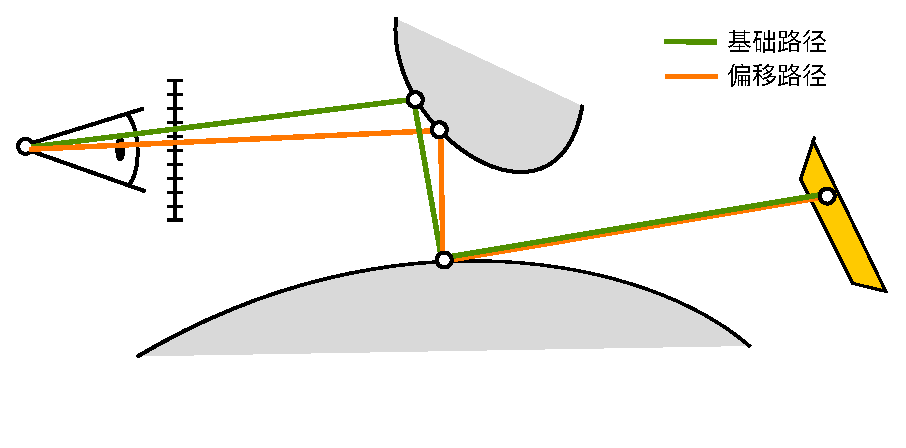
\includegraphics[width=0.65\textwidth]{figures/pt/shift-mapping.eps}
	\caption{梯度域渲染的核心就是在传统的路径采样的基础上,使用某种移位映射函数从基础路径产生一条偏移路径,然后以此计算两条路径之间的差异作为图像的梯度图像}
	\label{f:pt-shift-mapping}
\end{figure}

因此,我们需要使用另外的方式来计算梯度图像,当然这不应该使路径追踪的采样计算变得复杂。梯度域渲染使用一个移位映射(shift mapping)\myindex{移位映射}{shift mapping}来将一个基础路径(base path)\myindex{基础路径}{base path}映射到一个相邻像素的偏移路径(offset path)\myindex{偏移路径}{offset path},并以此来计算路径差异,如图\ref{f:pt-shift-mapping}所示(我们将在第\ref{sec:pt-gradient-analysis}节的傅里叶分析中看到移位映射应该尽可能使基础路径和偏移路径尽可能的相似,即使两者之间的差异更小来捕捉图像高频区域的变换特征,来使渲染的结果质量更好)。

移位映射使得上述的梯度计算变成一个单一路径的积分形式:

\begin{equation}\label{e:pt-gradient-equation}
\begin{aligned}
	\Delta_{i,j}&=\bigg( h(x)\star{\rm \int}_\Omega \bigg( f(x,\bar{p})-f(T_{ij}(x,\bar{p}))|T^{'}_{ij}| \bigg) {\rm d}\mu(\bar{p}) \bigg)(x_i)\\
	&=\bigg(h(x)\star{\rm \int}_\Omega g_{ij}(x, \bar{p}){\rm d}\mu(\bar{p}) \bigg)(x_i)
\end{aligned}
\end{equation}

\noindent 这里$T_{ij}$表示移位映射函数(shift mapping)\myindex{映射函数}{shift mapping},它使用确定性的方法将一个基础路径$(x,\bar{p})$映射为一个相邻的偏移路径$T_{ij}(x,\bar{p})$(移位映射相关的内容将在第\ref{sec:pt-gradient-mapping}节讨论),使得这两条路径足够的近似,并且它使得我们不需要增加额外的路径采样,如图\ref{f:pt-shift-mapping}所示。$|T^{'}|=|{\rm \partial} T/{\rm \partial} \bar{x}|$是移位映射函数$T$的雅可比行列式(Jacobian determinant)\myindex{雅可比行列式}{Jacobian determinant},它反映积分变量的变化。$g_{ij}(x,\bar{p})$表示一个路径差异函数(path difference function)\myindex{路径差异函数}{path difference function},用来作为梯度图像的被积函数。





\subsection{对称梯度和重要性采样}
可以证明,积分公式\ref{e:pt-gradient-equation}的估计是无偏的,当前仅对其移位映射是对称的。当一个基础路径与其偏移路径均可以被路径采样器采样时,我们称这样的一对基础-偏移路径对是对称的(symmetric)\myindex{对称的}{symmetric}。

很显然,实践上几乎不可能找到这样的移位映射函数使得所有路径对都是对称的。路径追踪技术保证路径空间的所有合法路径($f(x,\bar{p})>0$)都可以被采样,但是它不能保证这些基础路径的偏移路径也可以被采样,例如偏移路径可能被遮挡,导致其光照贡献值为0($f(T_{ij}(x,\bar{p})=0)$);另一方面,一些可以被采样的偏移路径($f(T_{ij}(x,\bar{p})>0$),其对应的基础路径可能贡献值为0($f(x,\bar{p})=0$),从而使得这种类型的偏移路径被完全忽略(因为传统路径追踪必须保证基础路径贡献值不为0),这就存在一些偏移路径无法被采样到,从而给梯度估计带来偏差。

由于路径采样的估计本身是无偏的,因此针对上述第二个问题,如果移位映射是可逆的(invertible)\myindex{可逆的}{invertible},则我们可以将路径采样得到的路径看做偏移路径,然后对其运用移位映射的逆来求其对应的基础路径。这种情况下,两个像素之间的梯度由两部分组成:由$i\to j$的前向移位映射(forward shift mapping)\myindex{前向移位映射}{forward shift mapping}和由$j\to i$的逆向移位映射(inverse shift mapping)\myindex{逆向移位映射}{inverse shift mapping},对这两个积分各自分配一个权重系数,\cite{a:ImprovedSamplingforGradientDomainMetropolisLightTransport}提出的新的对称梯度(symmetric gradient)\myindex{对称梯度}{symmetric gradient}公式为:

\begin{equation}\label{e:pt-symmetric-equation}
\begin{aligned}
	\Delta_{i,j}&=\bigg(h(x)\star{\rm \int}_\Omega w_{ij} g_{ij}(x, \bar{p}){\rm d}\mu(\bar{p}) \bigg)(x_i)\\
	&=\bigg(h(x)\star{\rm \int}_\Omega w_{ji} g_{ji}(x, \bar{p}){\rm d}\mu(\bar{p}) \bigg)(x_j)
\end{aligned}
\end{equation}

\noindent 我们暂时把权重系数$w_{ij}$和$w_{ji}$的计算放到稍后。上式意味着,对于路径采样得到的每一条路径,我们不仅需要将其当做基础路径求出水平和垂直两个方向上的偏移路径来求对应的梯度值,还需要将其当做偏移路径,并通过逆向移位映射来求出其对应的基础路径。因此,每个采样路径需要对周围4个像素进行梯度计算,其中两条偏移路径及两条逆向基础路径,如图\ref{f:pt-four-neighbors}所示。其计算的梯度对偏移距离为正值,对应式\ref{e:pt-symmetric-equation}中的第一项,对两条逆向基础路径为负值,对应式\ref{e:pt-symmetric-equation}中的第二项。

\begin{figure}
	\sidecaption
	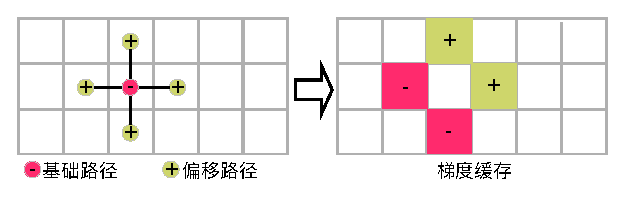
\includegraphics[width=0.65\textwidth]{figures/pt/four-neighbors}
	\caption{在对称梯度公式中,路径采样得到的每条路径需要对周围4个相邻像素计算梯度值,其中两条偏移路径和两条逆向映射基础路径}
	\label{f:pt-four-neighbors}
\end{figure}

对称梯度公式式\ref{e:pt-symmetric-equation}由两个积分公式组成,它表示梯度由两种不同的采样技术构成,对于多种不同的采样技术,一般我们需要使用复合重要性采样(multiple importance sampling)\myindex{复合重要性采样}{multiple importance sampling}方法将它们组合起来,即是根据某种规则将每种采样技术各自分配一个权重系数。在第\ref{sec:mc-balance-heuristic}节我们讨论了一般复合重要性采样技术的平衡启发式,由于移位映射的复杂性,本节我们将对式\ref{e:pt-symmetric-equation}表示的梯度公式使用另外一种启发式。

式\ref{e:pt-symmetric-equation}中的混合系数$w_{ij}$和$w_{ji}$非常复杂,\cite{a:ImprovedSamplingforGradientDomainMetropolisLightTransport}给出了详尽的解释。如图\ref{f:pt-symmetric-gradient}所示,$\Omega_i$和$\Omega_j$分别表示所有对相邻像素对$i$和$j$有贡献的路径空间,$T$表示$i$向$j$的移位映射,而$T^{-1}$表示$j$向$i$的逆向移位映射;$\Omega_{ij}$和$\Omega_{ji}$表示一对对称空间,在这个空间内的基础路径和偏移路径是互相对称的,即$\Omega_{ij}$内的基础路径对应的偏移路径位于$\Omega_{ji}$中,而$\Omega_{ji}$内的偏移路径对应的逆向基础路径位于$\Omega_{ij}$中(由此可以看出,当$\Omega_{ij}=\Omega_{ji}=0$时,梯度值变成两个相邻的基础路径之差,即回到式\ref{e:pt-gradient-equation});$\bar{\Omega}_i$和$\bar{\Omega}_j$表示非对称的空间,其中$\bar{\Omega}_i$内的基础路径对应的偏移路径对$j$的贡献为0,而$\bar{\Omega}_j$内的偏移路径对应的逆向基础路径对$i$的贡献为0。

\begin{figure}
	\sidecaption
	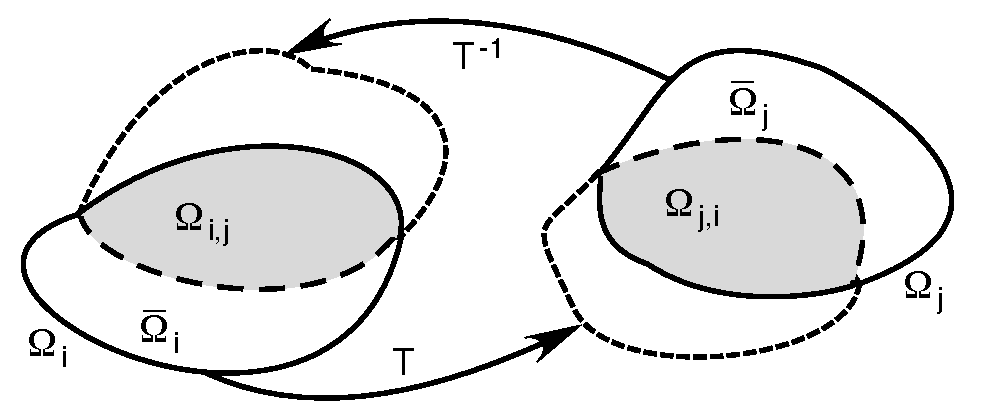
\includegraphics[width=0.55\textwidth]{figures/pt/symmetric-gradient}
	\caption{对称梯度相关的一些标记及概念:$\Omega_i$表示所有对像素$i$具有贡献的路径空间区域,区域$\bar{\Omega}_i$表示$\Omega_i$的子空间但是它不能够通过像素$j$的逆向移位映射采样,相反,$\Omega_{ij}$是能够被区域$\Omega_j$逆向映射到的}
	\label{f:pt-symmetric-gradient}
\end{figure}

通过上面的分析,式\ref{e:pt-symmetric-equation}中的权重系数$w_{ij}$和$w_{ji}$可以分为三种情况(当然首先满足$w_{ij}+w_{ji}=1$):

\begin{itemize}
	\item 偏移路径的贡献为0:即$\bar{\Omega}_i$空间内的基础路径,由于这些基础路径对应的偏移路径位于$\Omega_j$之外,所以$f(T(x,\bar{p}))=0$,这时我们设定$w_{ij}=1$,而$w_{ji}=0$。
	\item 基础路径的贡献为0:即$\bar{\Omega}_j$空间内的偏移路径,由于这些偏移路径对应的逆向基础路径位于$\Omega_i$之外,所以$f(x,\bar{p})=0$,这时我们设定$w_{ij}=0$,而$w_{ji}=1$。
	\item 基础路径和偏移路径的贡献均不为0:这即是对称路径所在的空间,即基础路径和偏移路径都可以被路径采样器采样得到,这种情况下我们使用下述的启发式。
\end{itemize}

对称空间内的基础-偏移对路径是对称的,即它们对梯度的贡献值均不为0,假设基础路径$\bar{x}$对应的概率密度函数为$p(\bar{x})$,则其对应的偏移路径的概率密度函数为$p(T_{ij}(\bar{x}))|T^{'}_{ij}|(\bar{x})$,所以根据复合重要性采样的平衡启发式(balance heuristic)\myindex{平衡启发式}{balance heuristic}可以得出$w_{ij}$的值(相应可以计算出$w_{ji}$的值)为:

\begin{equation}
	w_{ij}(\bar{x})= \cfrac{p(\bar{x})}{p(\bar{x})+p(T_{ij}(\bar{x}))|T^{'}_{ij}|(\bar{x})}
\end{equation}

\noindent 需要注意的是,上面的复合重要性采样还解决了另一个问题,即当移位映射的行列式$|T^{'}_{ij}(\bar{x})|$很大时,梯度估计的方差将会很大,上述公式使得这样的采样权重变为$1/|T^{'}_{ij}(\bar{x})|$,因此它取消了该部分梯度采样的巨大贡献,从而减小了梯度估计的方差。

根据本节内容,\cite{a:GradientDomainPathTracing}提供的梯度域路径追踪算法伪代码\footnote{\cite{a:GradientdomainpathtracingGPTandgradientdomainbidirectionalpathtracingGBDPTforMitsubarenderer}提供了基于Mitsuba渲染器的梯度域路径追踪算法实现。}如下:

\begin{lstlisting}[language=C++,mathescape]
//使用传统路径追踪采样算法得到所有基础路径
for all sampled base paths $\bar{x} = (x, \bar{p})$ {
	for all pixels $i$ where $h(x - x_i)$ > 0 {
		// 写入基础路径至主要图像中
		$I_i := I_i + h(x - x_i)f(\bar{x})/p(\bar{x} ̄)$
		for all neighbor pixels $j$ {
			$\bar{y}:= T_{ij} (\bar{x})$; 
			// 计算$w_{ij}(\bar{x})$
			$\Delta_{i,j}:=\Delta_{i,j}+w_{ij}(\bar{x})h(x-\bar{x})(f(\bar{x})-f(\bar{y})|T^{'}_{ij}|)$
		}
	}
}
	
for all $j$ 
	$I:=I/N; \Delta_{;j} := \Delta_{·,j}/N$
Reconstruct($I, \Delta_{.,.},\alpha$)
\end{lstlisting}

根据上述算法,我们已经讨论了怎样计算梯度图像,使用筛选的泊松方程重建图像还需要找出适当的梯度图像和参考图像的混合权重系数$\alpha$,这个最优的权重系数涉及对梯度域采样的傅里叶分析,我们将在下一节讨论。此外,我们还需要适当的移位映射算法来计算梯度值(第\ref{sec:pt-gradient-mapping}节)。






\subsection{梯度域的傅里叶分析}\label{sec:pt-gradient-analysis}
前面已经讨论了梯度域路径追踪算法的基本思路和过程,它实现起来也非常简单,只需要对已有路径追踪算法做少量修改即可实现。然而要想真正理解基于梯度场的图像重建带来的好处,我们必须对这个重建过程进行傅里叶分析,\cite{a:GradientDomainPathTracing}第一次提出了对梯度域渲染完整的傅里叶分析。

和传统路径追踪算法一样,梯度域渲染也是一个随机过程,因此衡量其估计质量的方法就是分析其估计误差。以下首先分析并比较梯度域图像和参考图像的均方差,然后分析重建图像的均方差并推导出最优的筛选泊松方差参数$\alpha$。





\subsubsection{梯度估计的误差分析}
为了简化分析过程,\cite{a:GradientDomainPathTracing}的傅里叶分析做了几个简化:

\begin{itemize}
	\item 假设分析图像是1D的,所以$x$代表了图像坐标空间的维度。
	\item 所有的路径空间积分参数都隐藏在路径$\bar{p}$中。
	\item 放大了方差计算,由于方差$V(x)=E[X^2]-(E[X])^2$,这里设期望$E[f(X)]=0$,因此方差被放大(即$V(x)=E[f(X)^2]$),这里$E[f(X)^2]$表示$f$的能量。
	\item 最后,这里的移位映射仅仅将图像坐标,即$x$,移动一个像素,而其他的所有参数保持不变,因此这里的$T$对应的雅可比矩阵为单位矩阵,其行列式值为1(即基础路径和偏移路径重合)。
\end{itemize}

这里由于$T(x,\bar{p})=(x-1,\bar{p})$,所以$g(x,\bar{p})=f(x,\bar{p})-f(x-,\bar{p})$,由此可以使用一个卷积来表示路径差异函数,即:$g(x,\bar{p})=(d\star f)(x,\bar{p})$,这里$d(x,\bar{p})=\delta(x)-\delta(x-1)$是一个差异算子(difference operator)\myindex{差异算子}{difference operator},它是两个脉冲函数的差。

空间域的卷积$g=d\star f$相当于频率域的乘积$G=DF$,$|G|^2$表示路径差异函数的能量谱(power spectrum)\myindex{能量谱}{power spectrum},它与$|F|^2$的关系\footnote{关于$d$的傅里叶变换可以参见\cite{a:SupplementalMaterialforGradientDomainPathTracing}的推导。}为:

\begin{equation}
\begin{aligned}
	|G(\omega_x,\omega_{\bar{p}})|^{2}&=(2-2\cos(2\pi\omega_x))|F(\omega_x,\omega_{\bar{p}})|^{2}\\
	&=|D(\omega_x,\omega_{\bar{p}})|^{2}|F(\omega_x,\omega_{\bar{p}})|^{2}
\end{aligned}
\end{equation}

\noindent \cite{a:GradientDomainPathTracing}通过将路径采样过程当做一个泊松过程,参考图像和梯度图的方差可以表示为:

\begin{equation}
	\begin{aligned}
		|\epsilon_F (\omega_x,\omega_{\bar{p}}) |^2 &= \cfrac{1}{n}||F||^2 \\
		|\epsilon_G (\omega_x,\omega_{\bar{p}}) |^2 &= \cfrac{1}{n}||G||^2
	\end{aligned}
\end{equation}

\noindent 它们反比于采样密度$n$,其中$||F||^2$和$||G||^2$均为常数,表示信号的总能量,即:

\begin{equation}
\begin{aligned}
	||F||^2 &={\rm \int} |F(\omega_x,\omega_{\bar{p}})|^{2}{\rm d}\omega_x {\rm d}\omega_{\bar{p}}\\
	||G||^2 &={\rm \int} (2-2\cos(2\pi\omega_x))|F(\omega_x,\omega_{\bar{p}})|^{2} {\rm d}\omega_{\bar{p}}	
\end{aligned}
\end{equation}

\noindent 由此可以看出,积分$||F||^2$和$||G||^2$的不同在于差异算子引入的系数$|D(\omega_x)|^2=(2-2\cos (2\pi\omega_x))$,因此像素误差$|\epsilon_F |^2$和$|\epsilon_G |^2$之间的差异取决于图像中低频和高频部分的相对数量。对于梯度图估计,$|D(\omega_x)|^2$的取值范围在$0-4$之间,在最好的情况下,所有的能量处于低频部分,由于$|D(\omega_x)|$系数很小,因此梯度能量可以变得任意小,即是梯度估计的误差变得任意小,如图\ref{f:pt-gradient-error}所示。

\begin{figure}
	\sidecaption
	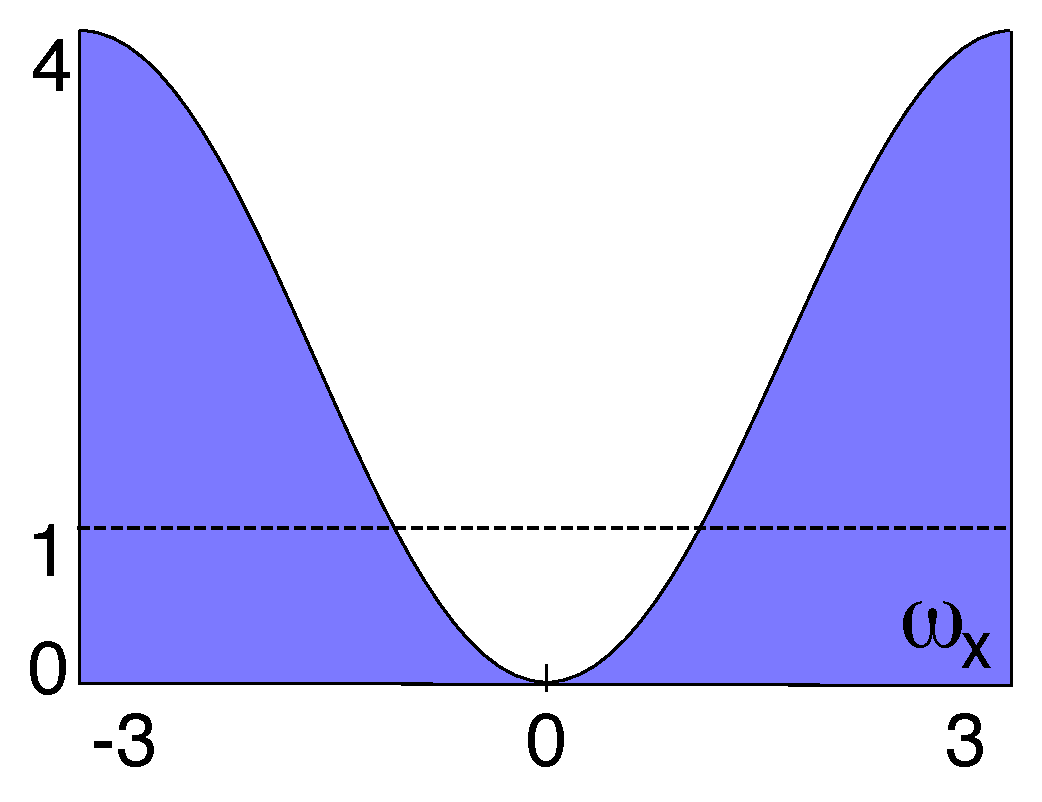
\includegraphics[width=0.45\textwidth]{figures/pt/gradient-error}
	\caption{梯度估计的误差在低频区域内最小,随着频率的增加而成余弦增加,虚线表示像素图像的误差$|\epsilon_F(\omega_x)|^2$,它在采样数量$n$给定的情况下为常数,梯度估计的误差最大为像素图像估计误差的4倍(纵轴表示像素图像误差的倍数)}
	\label{f:pt-gradient-error}
\end{figure}

而在给定采样数量$n$的情况下,像素图像的误差$|\epsilon_F(\omega_x)|^2$为一常数(如图\ref{f:pt-gradient-error}所中的虚线所示),在后面的图像重建分析中,我们就将进一步根据像素图像和梯度图像的误差特征来分析重建图像的误差。






\subsubsection{重建图像误差分析}
我们已经知道,梯度域路径追踪算法的思路就是在生成每条路径采样的时候,同时计算一个梯度图和一个像素图像,然后利用前面讨论的筛选泊松方程重建图像。在前面我们已经得出了像素图像和梯度图像的误差的表达式,根据筛选的泊松重建方程,我们可以得到重建图像的误差(使用梯度图像和像素图像的误差表述)为:

\begin{equation}
	|\epsilon_{R_{\alpha}}(\omega_x)|^2= \cfrac{1}{n} \cfrac{\alpha^4||F||^2 +|D(\omega_x)|^2||G||^2}{(\alpha^2 + |D(\omega_x)|^2 )^2}
\end{equation}

\noindent 在上式中,如果设$\alpha=\infty$,则此时相当于仅考虑像素图像,因此重建图像的误差变为$\epsilon_{R_\infty}=||F||^2/n$;我们更感兴趣的是如果设$\alpha=0$,此时意味着仅考虑梯度图像,则重建图像的误差变为:

\begin{equation}
\begin{aligned}
	|\epsilon_{R_0}(\omega_x)|^2 &=1/n\cdot||G||^2/|D(\omega_x)|^2\\
	&=1/n\cdot||G||^2/(2-2\cos(2\pi\omega_x) )
\end{aligned}
\end{equation}

上式表述的误差呈现两个特征:其误差的大小取决于常数$||G||^2$(即梯度图像的能量),而其误差的变化曲线取决于$1/|D(\omega_x)|^2$。对于后者,我们将图\ref{f:pt-gradient-error}除1得到图\ref{f:pt-reconstruction-error},因此如果我们仅使用梯度图像来重建真实图像,则与梯度图像本身的误差特征相反,它在高频区域的能量最低,因此估计的误差最低。因此,重建图像中能够从梯度估计中受益(误差比像素图像更低)的频率取决于梯度图像能量和像素图像能量的比值$||G||^2/||F||^2$,例如在图\ref{f:pt-reconstruction-error}中高频部分的误差比像素图像的误差要低得多,而低频部分则大于像素图像的误差(最大多至4倍)。

图\ref{f:pt-reconstruction-error}还呈现一个重要特征,那就是梯度图像部分贡献的误差在低频部分的范围很窄,它在经历短暂的低频高误差范围带之后,迅速进入高频低误差范围,使其拥有较大的低误差范围。实际上,大部分图像都由于阴影遮挡,物体边缘,颜色变化等等因素使得其图像分布呈现较大的高频带,因此梯度域追踪技术能够减小传统蒙特卡洛方法的方差。

\begin{figure}
	\sidecaption
	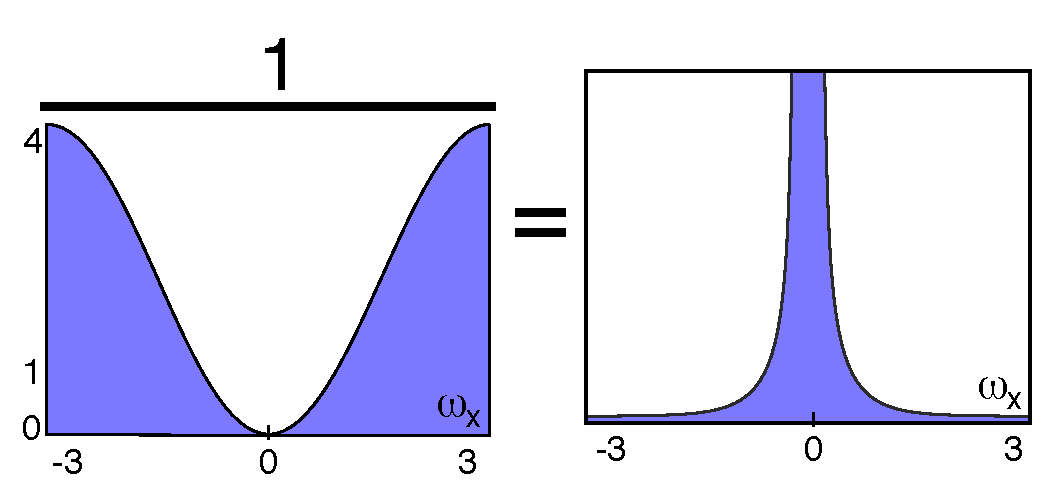
\includegraphics[width=0.6\textwidth]{figures/pt/reconstruction-error}
	\caption{和梯度图估计的误差分布相反,筛选泊松重建的图像在高频区域的误差最小,并且高误差在低频区域的范围很小,经历短暂的低频区域后迅速减少,大部分高频区域的误差都很低}
	\label{f:pt-reconstruction-error}
\end{figure}

根据目前的分析,在重建的图像中,像素图像(传统蒙特卡洛方法)部分贡献的误差为常数,梯度图像对误差的贡献在高频部分远远小于像素图像误差,而在低频部分大于像素图像误差。因此,理想情况下,我们希望对像素图像使用一个低通过滤器(low-pass filter),而对梯度图像使用一个高通过滤器(high-pass filter),这样就的组合就能够在高频部分大大减少误差,而在低频部分至少保持传统路径采样算法的误差,如图\ref{f:pt-screen-poisson-reconstruction}所示。

\begin{figure}
	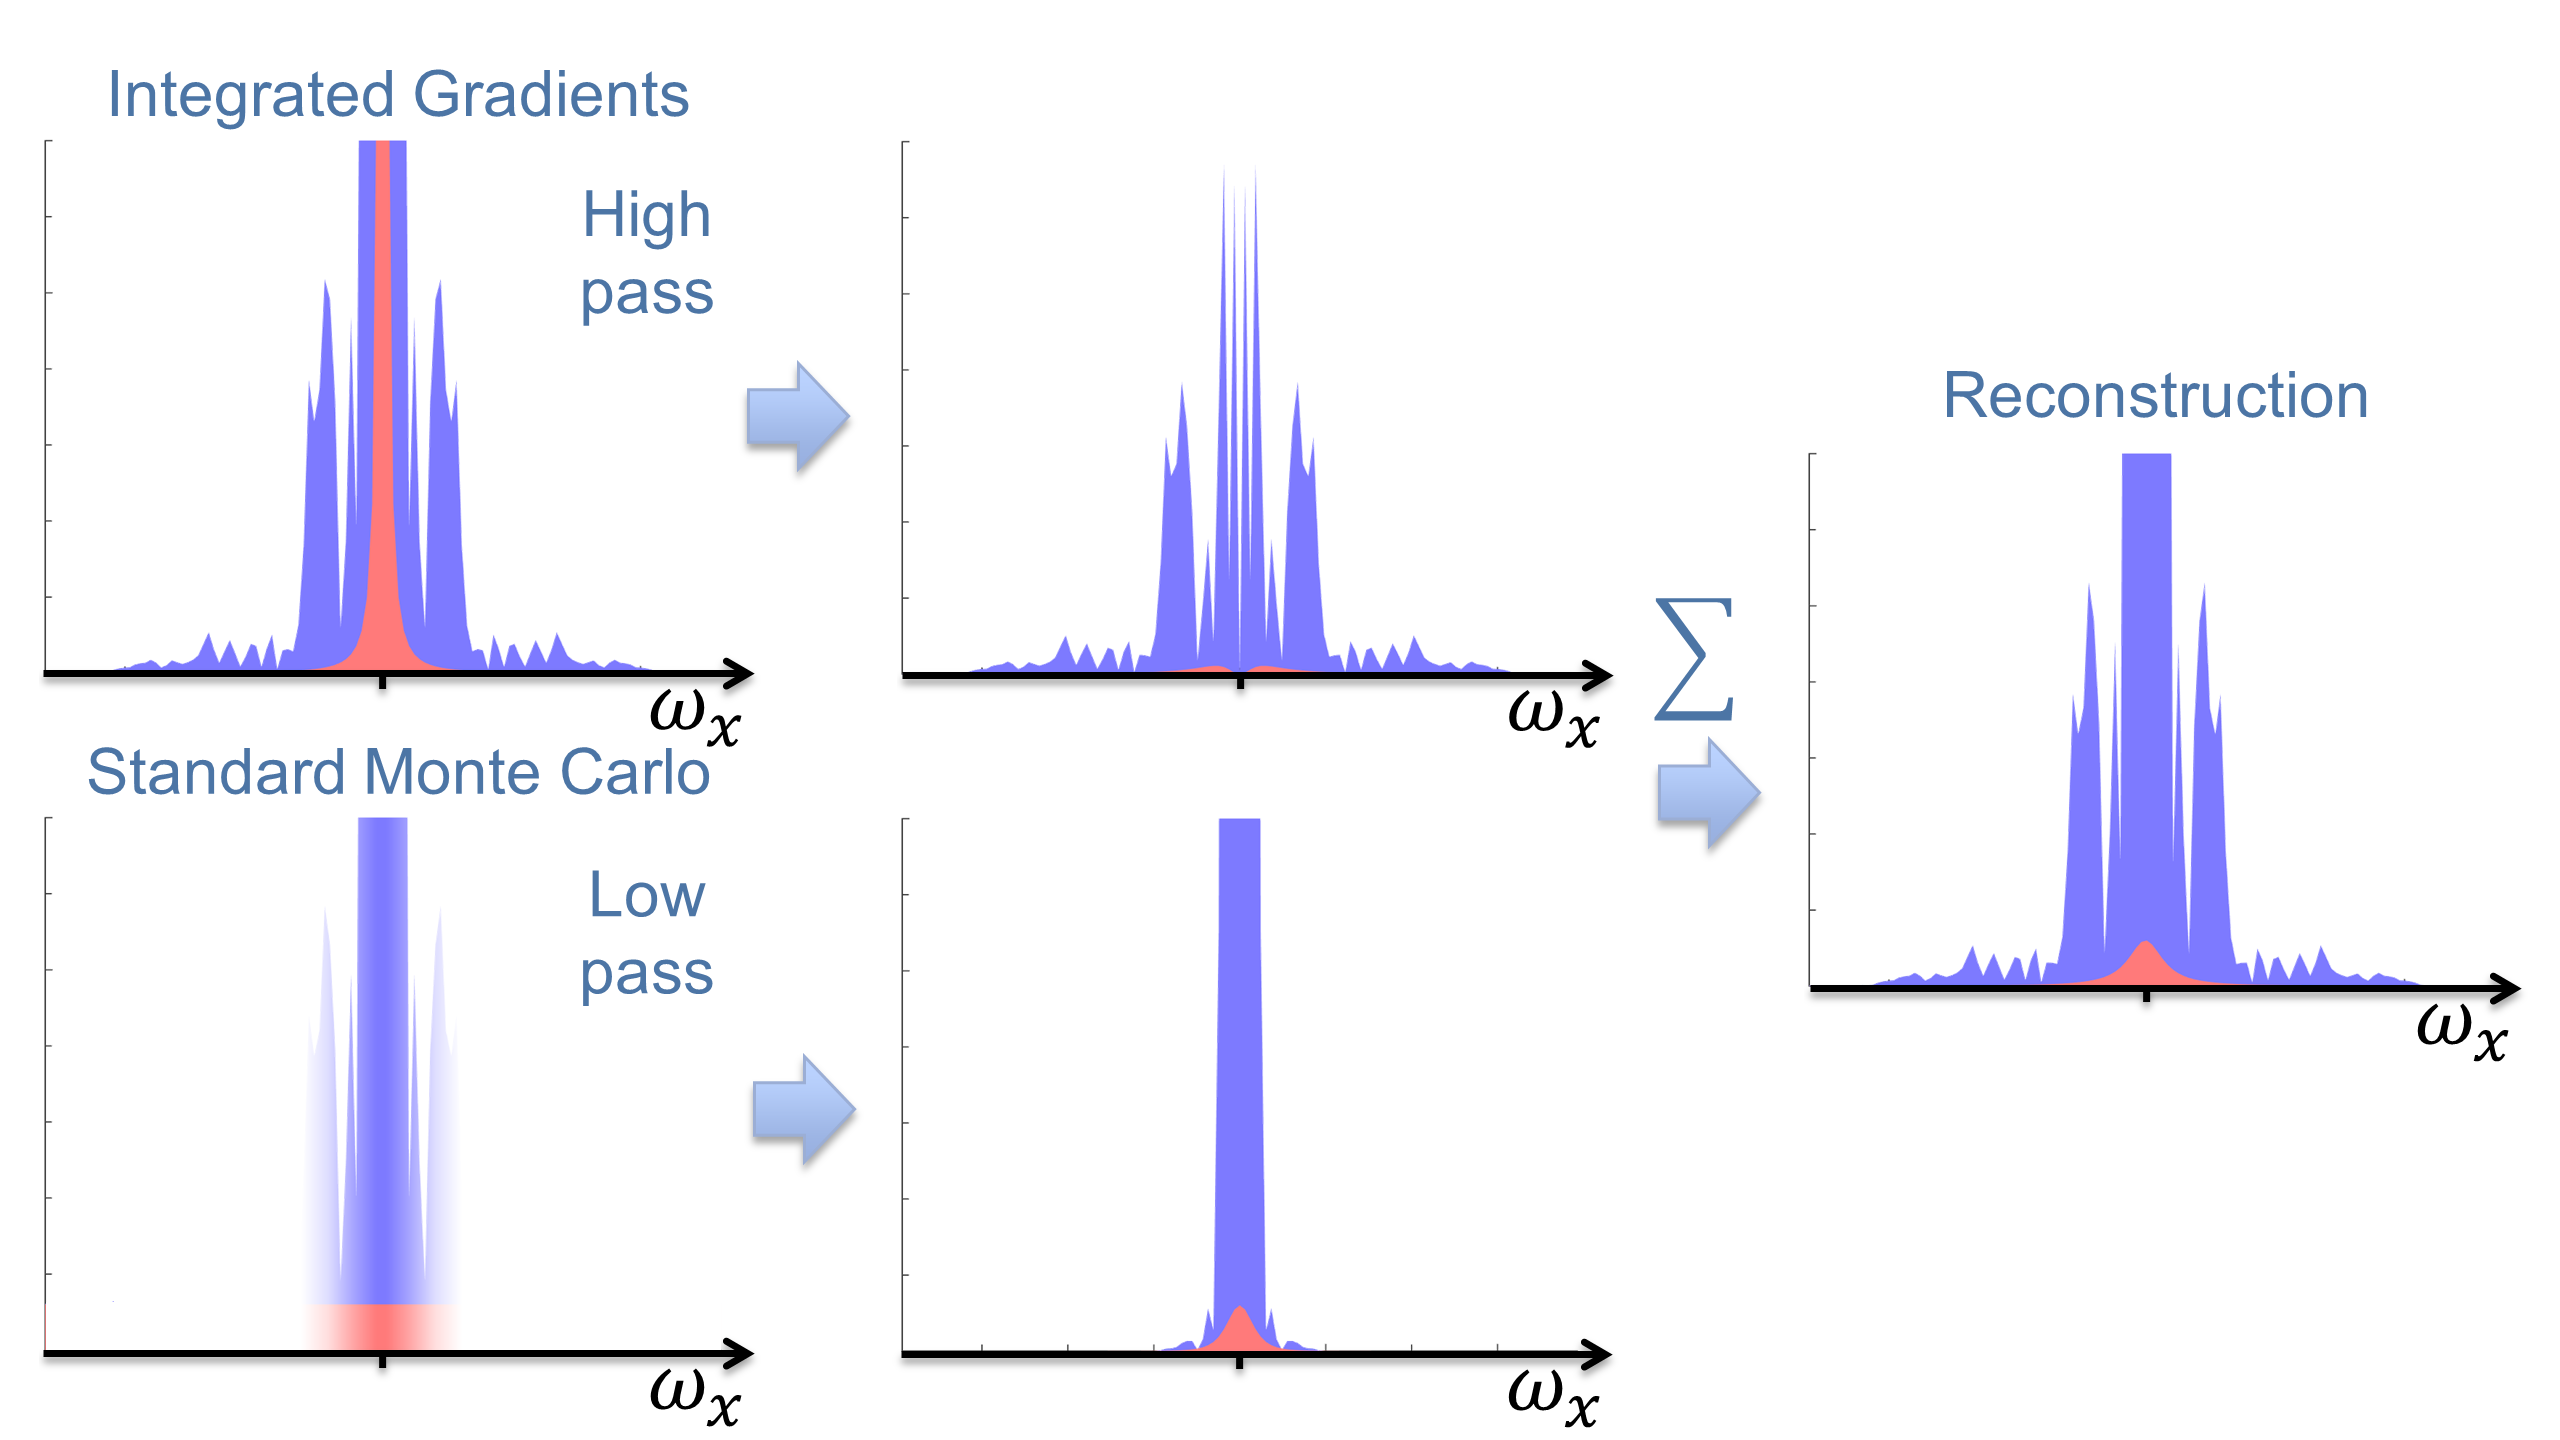
\includegraphics[width=1.\textwidth]{figures/pt/screen-poisson-reconstruction}
	\caption{根据梯度图像和像素图像在对基于筛选泊松方程重建图像误差的贡献,我们希望对像素图像使用低通过滤器,对梯度图像使用高通过滤器,来使重建图像的误差更低}
	\label{f:pt-screen-poisson-reconstruction}
\end{figure}

\cite{a:GradientDomainPathTracing}说明,图\ref{f:pt-screen-poisson-reconstruction}的过程正是式\ref{e:screen-poisson-reconstruction}所表示的筛选泊松重建图像在频率域空间的描述,并且最优的混合权重系数为$\alpha^{2}_{\star}(\omega_x)=||G||^2/||F||^2$,此时重建图像的误差用梯度图和像素图像的能量表示为:

\begin{equation}
	|\epsilon_{R_{\alpha_{\star}}}(\omega_x)|^2= \cfrac{1}{n} \cfrac{||G||^2 ||F||^2}{||F||^2|D(\omega_x)|^2+||G||^2}
\end{equation}

\noindent 重建图像误差的另一个特征在于其大小取决于常数$||G||^2$(即梯度图像的能量),因此梯度图像的能量必须尽可能$||G||^2$小,其实就是用于产生偏移路径的移位映射函数必须使得两条路径尽可能地相似,这样就是梯度图像的总能量越小。并且基础路径和偏移路径越相似,梯度图像越能捕捉更多高频区域,因此进一步减小了方差,下一节我们就将讨论一种比较高效的移位映射函数。





\subsection{移位映射}\label{sec:pt-gradient-mapping}
从上一节的傅里叶分析中可以看出,梯度域渲染的质量依赖于其使用的移位映射函数,其产生的偏移路径和基础路径越相似,则生成的梯度图像的能量$||G||^2$越低,因此重建图像的误差越低。\cite{a:GradientDomainMetropolisLightTransport,a:ImprovedSamplingforGradientDomainMetropolisLightTransport}使用本章后面第\ref{sec:pt-manifold}节讨论的基于流形突变的光照传输技术来生成偏移路径,其生成偏移路径的成本相对较高,\cite{a:GradientDomainPathTracing}使用一个更简单高效的策略来生成偏移路径。

两条(顶点数量相同的)路径越相似,则它们在空间几何上越相似,并且每个对应顶点的BSDF反射系数变化不大。因此最自然的想法是尽可能地重用基础路径中的顶点,即从一个偏移像素位置开始的偏移路径应该尽可能早地与基础路径的顶点连接重合。然而在重合的过程中需要注意,当表面为光泽面时,其BSDF随方向的变化较大,直接连接可能产生较大的差异。

\begin{figure}
	\sidecaption
	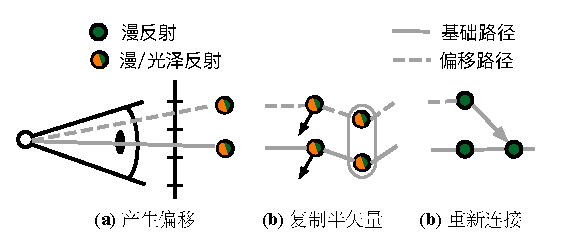
\includegraphics[width=0.65\textwidth]{figures/pt/copy-shift-mapping}
	\caption{一个简单的移位映射:(a)首先在屏幕空间偏移一个像素产生偏移路径,(b)对于光泽面,直接复制基础路径对应的半矢量用来决定光泽反射的方向;(c)对于漫反射表面,直接连接偏移路径的当前顶点和基础路径的下一个顶点}
	\label{f:pt-copy-shift-mapping}
\end{figure}

\cite{a:GradientDomainPathTracing}使用的移位映射函数具有以下三个步骤:

\begin{enumerate}
	\item 首先从摄像机开始,在屏幕空间从基础路径偏移一个像素产生偏移路径,这产生一个场景表面中的顶点,如图\ref{f:pt-copy-shift-mapping}(a)所示。
	\item 如果基础路径当前或者下一个顶点位于光泽面,为了避免产生较大差异,则根据BSDF重新生成一个新的路径方向,如图\ref{f:pt-copy-shift-mapping}(b)所示。但是为了避免使用光线追踪方法产生新顶点的成本,这里直接复制对应基础路径中顶点的半矢量(half vector)\myindex{半矢量}{half vector}用来决定下一个顶点的方向。该过程需要注意的是检查路径的可逆性,因为如果该操作不可逆则会给估计带来偏差,这通过两方面来满足:首先,如果偏移路径的下一个新的顶点和其对应的基础路径具有不同的表面属性,则该映射是不可逆的;其次,折射方向经过移位映射后位于全反射方向时,该映射也是不可逆的。对于这些不可逆的映射,偏移路径被直接丢掉,即基础路径的权重$w_{ij}=1$。
	\item 如果偏移路径的当前顶点,以及基础路径的当前和下一个顶点均位于漫反射表面,则直接连接偏移路径当前顶点和基础路径下一个顶点。
\end{enumerate}

这种简单的移位映射算法实际上主要是基于路径每个顶点的局部特征,即每个顶点局部很小范围内的顶点在几何特征及BSDF反射函数变化不大,因此直接复制半矢量并不会导致过大的差异,同时该移位映射算法仍然满足对称性。


\cite{a:GradientDomainPathTracing}还提供了上述移位映射函数雅可比行列式(Jacobian determinant)\myindex{雅可比行列式}{Jacobian determinant}的计算,这里不再复写。\cite{a:GradientdomainpathtracingGPTandgradientdomainbidirectionalpathtracingGBDPTforMitsubarenderer}提供了基于Mitsuba渲染器的梯度域路径追踪的实现代码。此外,\cite{a:Gradient-DomainBidirectionalPathTracing}还提供了基于双向路径追踪算法的梯度域路径追踪算法,由于该算法的移位映射函数采用与\cite{a:ImprovedSamplingforGradientDomainMetropolisLightTransport}类似的基于流形突变的映射方法,我们将这部分内容放在第\ref{chp:mlt}章讨论。




	


\begin{comment}
	

\subsection{采样技术}
Some very promising importance sampling techniques have re- cently been developed specifically for path tracing: “hero” wavelengths [99, 136] can be used for e cient spectral rendering (i.e. simulating more wavelengths than the usual red, green, and blue components), and advanced next-event estimation [42] can reduce noise in caustics. The images in Figure 5.2 illustrate these two techniques; both images were rendered with Weta’s in-house renderer Manuka. There has also been a wealth of new sampling techniques developed specifically for volumes, which we discuss in Section 5.3.2.

\subsection{采样模式}
简要介绍,clumpling导致收敛慢

\end{comment}









\section{提高光线追踪算法的效率}\label{sec:pt-efficiency}
到目前为止,我们的焦点都是在路径采样算法本身上。本章最后一部分,我们将抛开采样算法,简单讨论一下这些算法在硬件层面的执行和优化。

毫无疑问,路径追踪算法的计算量非常大,它需要非常巨量的路径数量来减少方差,而每条路径要经过多次遮挡计算,直接光采样,BSDF反射计算,纹理采样等,计算成本非常高。然而抛开这些固有的因素,在硬件算法执行层面,路径追踪算法的低效很大程度上与其基本算法的结构相关。例如光线树形成的递归路径采样既不符合现代处理器的管线执行模型,同时在读取内存时也不能有效地隐藏低带宽和高延迟。

本节将通过分析和调整基础路径追踪算法的基础结构,使之符合现代处理器的一些特征,来提升路径追踪算法的执行效率,这些处理器层面的算法优化对于现代工业中路径追踪渲染器的效率非常关键,例如Disney的Hyperion渲染器,有些路径追踪渲染器甚至可以在某些几何复杂度下达到实时渲染的性能。






\subsection{处理器执行模型小结}
本节首先对以下会用到的处理器执行模型进行简单总结,更详细的知识请读者复习第2章的内容。

现代处理器几乎都以冯·诺依曼提出的处理器结构为基础,在该结构中,处理器由四部分组成:一个用于进行二进制运算的算术逻辑单元,一个用来高速存储指令和数据的寄存器组,一个用来控制指令读取的控制单元,以及一个用于存储所有指令和数据的内存。

在冯·诺依曼模型中,处理器从内存中将指令和数据(包括地址)读取到寄存器 并解码,然后执行该指令。寄存器在物理设计上靠近处理器,它是计算机所有存储设 备中具有最快存取速度(通常 1 个 CPU 时钟周期)的存储设备,但是它通常只有有 限的容量 (几千 byte),所以当寄存器中的指令或数据执行完毕后,就需要向主存读取数据。

这个模型看起来并不复杂,然而在现代处理器的发展当中,算术逻辑单元的计算速度得到了非常大的发展,例如现代处理器的运行速度通常可以高达4GHz,而内存的发展则主要集中在容量而不是传输速度上,这就导致处理器需要花费更多时间用于等待寄存器从内存读取数据,其导致了资源和时间浪费。

现代处理器使用多种系统或机制来弥补由于内存传输速度带来的瓶颈,这些系统或机制也成为任何针对处理器硬件进行算法优化的重要方面,本节首先列出这些因素,然后在后面的讨论中能够更好地理解针对这些因素进行算法优化的原理和思路。




\paragraph{内存读取}
高速存储芯片非常昂贵,为了在制造成本和读取速度之间取得平衡,现代处理器使用一个多级的缓存系统来克服数据传输带来的延迟。在这个多级缓存系统当中,越靠近寄存器的缓存具有更快的速度,同时也具有更小的存储空间,例如L1缓存的大小通常只有16KB或32KB大小,但是读取速度只有几个CPU时钟周期,L3级缓存则可能多达几兆字节大小,但是往往需要几百个时钟周期的读取时间。

缓存系统的主要工作原理包括局部性原理和预取技术。首先,局部性原理包括时间局部性和空间局部性,例如当前指令的相邻后续指令要访问的数据,可能正位于当前内存数据在内存地址的附近,这就是空间局部性;而当前访问的数据很可能还要被后续相邻的指令访问,例如在一个函数内的局部变量,或者一个循环体内的数组,这就是时间局部性。利用局部性原理,我们可以一次性从下一级缓存中读取相对较大的一块数据,它可以被尽可能多的指令使用,这样就避免每条指令的执行都需要寄存器从主存中读取数据,并且通过后面的预取技术,理想情况下,可以保证寄存器想要的数据始终处于L1级缓存上。

当需要读取的数据不在最近一级的缓存上时,就需要从更下一级缓存读取数据,这称为缓存失效,它带来更大的数据传输延迟,因此是需要极力避免的。缓存系统的第二大工作原理即预取技术就是用来尽量避免缓存失效的几率。各级缓存是按照一个固定大小从下一级缓存一次性读取数据的,这称为一个缓存行,预取技术通常根据局部性原理提前读取当前数据附近的数据到缓存中,同时它也会根据一些规则(如最近最少使用算法)替换一些被认为不重要的缓存数据,通过这样来减少缓存失效的几率,这样整个缓存系统就在动态地根据指令调整数据,以隐藏数据直接由主存到寄存器的传输延迟。

上述的缓存系统对算法结构要求访问的数据应该尽可能连续,线性或相邻的数据访问顺序能够大大减少数据传输的延迟,减少处理器等待的时间,大大提高处理器的利用率。然而,在光线追踪算法中,一条光线经过与表面交互后可能反射或折射到任意方向,这就造成对数据读取的严重不连续,因此本节讨论的很多方法就是用于改善这种情况。





\paragraph{指令执行}
程序指令和数据在内存系统中的最后一站称为寄存器,它有着最快的读取速度(通常一个CPU时钟周期)和最小的存储空间(其大小通常按位计算)。

一个处理器通常有多个不同类型的寄存器,这个类型是根据其包含的数据类型或者执行于该数据上的指令类型划分的。例如,数据寄存器(data registers)\myindex{数据寄存器}{data registers}可以用来存储整形或浮点型等数据类型的数据,地址寄存器(address registers)\myindex{地址寄存器}{address registers}专门用于存储一个可以直接被指令访问的内存地址,而指令寄存器(instruction register)\myindex{指令寄存器}{instruction register}存储当前正在被执行的指令数据,更多关于寄存器的知识可以参考脚注资源\footnote{\url{https://en.wikipedia.org/wiki/Processor_register}}。

矢量寄存器(vector registers)\myindex{矢量寄存器}{vector registers}是一组特殊的寄存器,它们存储一个某个基础类型的矢量数据供SIMD指令执行。SIMD(single instruction, multiple data)是一类弗林分类法\footnote{\url{https://en.wikipedia.org/wiki/Flynn\%27s\_taxonomy}}(Flynn's taxonomy)\myindex{弗林分类法}{Flynn's taxonomy}中的并行处理器架构,它将一个相同的指令同时并行地执行于多个相同数据类型的数据之上,因此它能够实现数据级别的并行,SIMD指令对于矢量操作非常高效,它大大减少了寄存器从缓存读取或存储数据的时间。

矢量寄存器存储的基础数据分量的个数通常是4个,8个或更多,例如在OpenGL中一个矢量通常是由4个分量组成,一共128位,每个分量是一个32位的浮点值。算法通常要根据处理器支持的矢量寄存器分量的个数来调整数据结构,使之能够充分利用SIMD指令的计算效率。
 
除了SIMD指令之外,由于现代处理器指令执行通常是管线化的,因此当出现条件分支时,如果预测判断失败则将导致指令执行的浪费,从而影响计算性能。而对于GPU,由于它并不是为了执行串行代码而设计的,而是为了高效执行大量的并行计算,因此并没有如CPU那样复杂的硬件实现分支预测功能,这回导致GPU会对每个分支都完整的执行,从而导致每个时钟周期都有部分处理器资源被浪费。例如,当一条SIMD指令同时计算多个顶点的着色,如果这些顶点使用不同的材质,则可能导致分支。所以,好的分支处理也是算法优化的重要方面。

此外,由于路径追踪算法中的每条路径都是相互独立的,所以线程级别的并行通常比较简单,例如大部分都基于屏幕空间的划分来分配线程,而指令级别的并行要复杂得多,它涉及对算法基础结构的修改,所以本章后面并不对线程级别的并行做太多讨论。






\subsection{加速遍历的基元结构}
 为了计算一条光线与场景中物体表面的交点,每条光线需要遍历场景中的所有基元(primitives)\myindex{基元}{primitives},例如所有物体网格的所有三角形面,若场景中所有的基元数量为$N$,则每条光线相交计算的复杂度为$O(N)$。因此,路径追踪算法中光线/基元相交计算的成本非常高,针对光线相交计算的基元加速数据结构成为光线追踪算法中重要的组件。

场景所有基元的加速结构可以分为两大类:空间细分(spatial subdivisions)\myindex{空间细分}{spatial subdivisions}和物体层次结构(object hierarchies)\myindex{物体层次结构}{object hierarchies}。空间细分是对基元所在的空间进行递归地划分,与某个空间相交的基元则被存储到该部分空间区域对应的结构中。在这种情况下,一个基元(或物体)可能被存储到多个细分空间中,同时某些空间也可能不包含任何基元。

常见的基于空间细分的加速结构包括:

\begin{itemize}
  \item \textbf{八叉树}(OCTREES)\myindex{八叉树}{OCTREES}:如图\ref{f:pt-spatial-subdivisions}(a)所示(这里显示的是一个八叉树的一个2D平面),一棵八叉树从包围整个场景的一个立方体开始,递归地将每个立方体细分为8个子立方体,直到满足某个终止条件。
  \item \textbf{二叉空间分割}(BSPS)\myindex{二叉空间分割}{BSPS}:如图\ref{f:pt-spatial-subdivisions}(b)所示,二叉空间分割递归地每次使用一个分割平面将空间细分为两个部分,虽然分割平面的方向是没有限制的,但是实践中通常将该平面与坐标轴对齐,这种坐标对齐的二叉空间分割称为k-d树(k-dtree)\myindex{k-d树}{k-d tree},如图\ref{f:pt-spatial-subdivisions}(c)所示(我们将在下一章第\ref{sec:pm-photon-storing}节更详细地讨论k-d树)。
\end{itemize}

\begin{figure}
	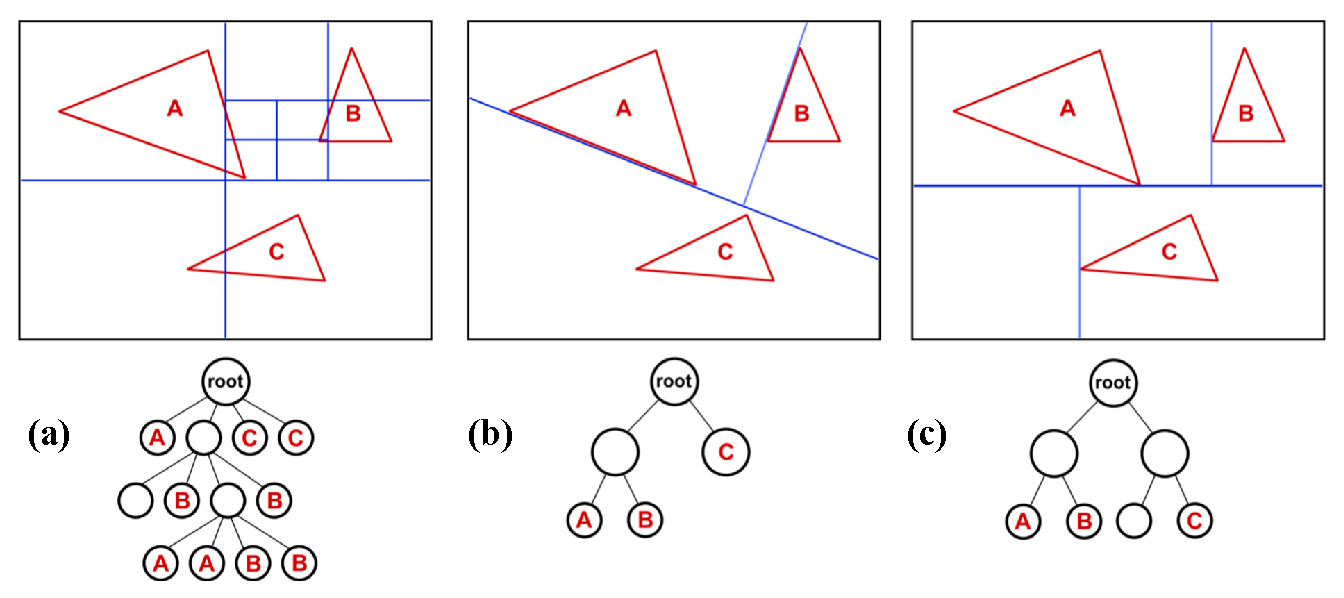
\includegraphics[width=1.\textwidth]{figures/pt/path-17-1}
	\caption{几种常见的空间细分方法,这里仅展示2D平面中的效果:(a)八叉树,(b)二叉空间分割及(c)k-d树}
	\label{f:pt-spatial-subdivisions}
\end{figure}

物体层次结构则是对基元(而不是空间)进行划分,在这种情况下,处于不同节点的基元所在的空间可能具有重叠部分。常见的物体层次结构划分如:

\begin{itemize}
	\item \textbf{包围盒层次结构}(Bounding volume hierarchy,BVH)\myindex{包围盒层次结构}{Bounding volume hierarchy},如图\ref{f:pt-object-subdivisions}(a)所示,BVH递归地对基元(或物体)列表进行划分,并在每一层级存储子树的AABB包围空间,这些分割面通常是与坐标轴对齐的(axis-aligned)。处于同一级的相邻两个节点的包围空间是可能会重叠的,但是每个节点内的基元数量不会为空。大部分实现使用将BVH实现为一个二叉树(binary tree)\myindex{二叉树}{binary tree},但是其他一些实现使用更大宽度的BVH,例如本章后面将会讨论的一些算法使BVH的宽度与处理器SIMD指令的长度一致,来利用SIMD指令对节点进行高效遍历。
	\item \textbf{包围间隔层次结构}(Bounding Interval Hierarchy,BIH)\myindex{包围间隔层次结构}{Bounding Interval Hierarchy}, 如图\ref{f:pt-object-subdivisions}(b)所示,BIH和BVH有些类似,但是与BVH存储一个完整的包围盒不同,BIH仅存储某个轴方向上的一个间隔。
\end{itemize}

\begin{figure}
	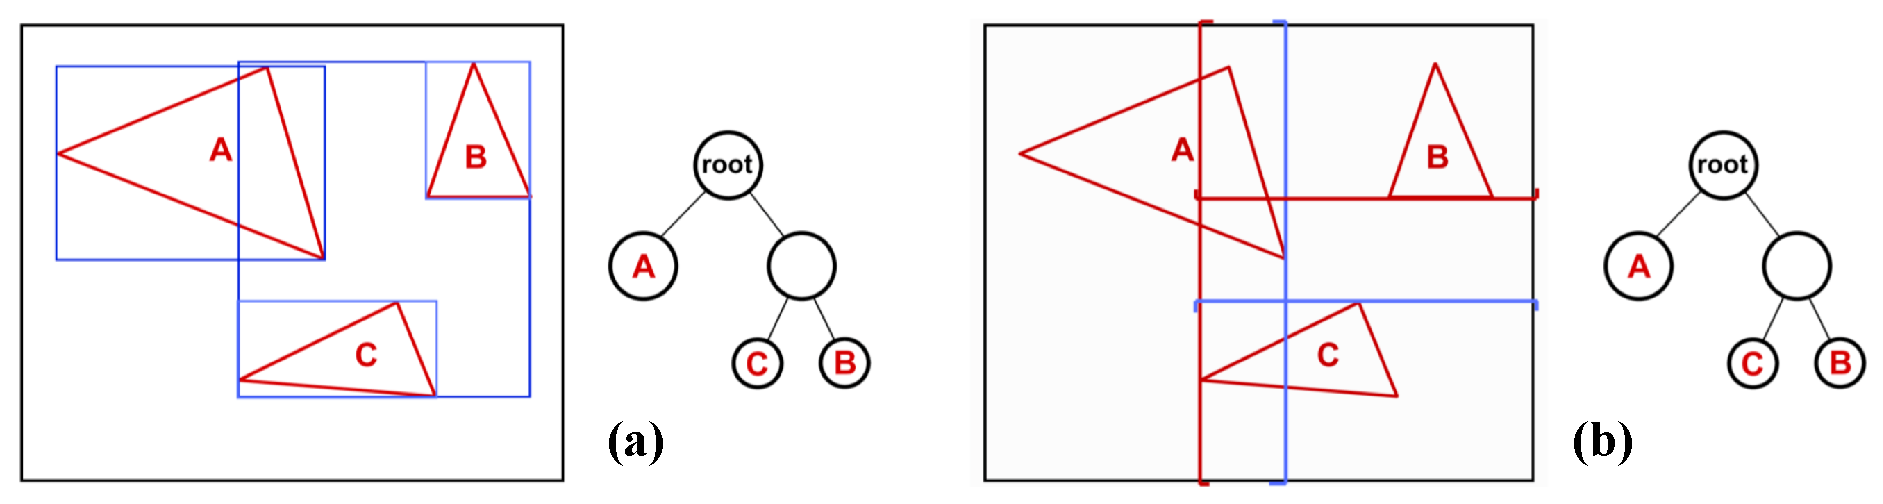
\includegraphics[width=1.\textwidth]{figures/pt/path-17-2}
	\caption{物体层次结构:(a)包围盒层次结构和(b)包围间隔层次结构}
	\label{f:pt-object-subdivisions}
\end{figure}

由于k-d树直接存储空间关系,因此对于静态的场景,它往往具有更快的光线相交计算的速度。但是在实践中,BVH的使用更普遍,这有两点原因:首先因为大部分场景使用一个物体层级结构来描述场景中的物体及其空间关系,因此这些物体本身的包围盒成为很好的细分的依据,这使得BVH结构的构建要比k-d树要高效得多;其次,每个物体可以表示为BVH的一个节点,所以这使得我们可以很容易地对BVH结构进行动态更新,如\cite{a:RayTracingDeformableScenesUsingDynamicBoundingVolumeHierarchies}等。

当然,实践中,基于空间的细分和基于物体的细分都有广泛的使用,也很难通过一些单一的因素来评估孰优孰劣,本章后面的内容我们将仅讨论BVH相关的内容,感兴趣的请读者自行查阅空间细分相关的资料。

另外需要注意的是,尽管看起来对象级别的层次划分对于BVH结构的建立有帮助,但是实际上BVH仅存储和基元相关的信息,它可能甚至不知道每个基元属于哪个对象。








\subsubsection{BVH的构建}
一个BVH结构可以拥有任意数量的分支因子(branching factor)\myindex{分支因子}{branching factor},尽管有一些比较通用的BVH构建方法,实践中大部分解决方案都是先生成最简单的分支因子为2的BVH,称为BVH2,然后使用后面会讨论的收缩和分离方法将此BVH2转化为分支因子为n的BVHn结构。

跟树形结构的搜索算法一样,树形层次结构的构造影响着光线追踪的效率。对于BVH结构,各个基元可以按照不同的方式进行分割,每种分割方法都将导致不同的计算时间。这里我们介绍一种比较简单同时也是使用比较广泛的一种分割方法\cite{a:RayTracingDeformableScenesUsingDynamicBoundingVolumeHierarchies},称之为表面面积启发式(surface area heuristic,SAH)\myindex{表面面积启发式}{surface area heuristic}。

SAH基于一个假设,即光线是均匀分布的,并且基元之间是不相交的,这样BVH中每个节点进行相交计算的时间成本正比于它的包围盒的面积。为了确定最优的分割位置,\cite{a:Automaticcreationofobjecthierarchiesforraytracing,a:Heuristicsforraytracingusingspacesubdivision}使用一个表面面积启发式成本函数来度量一种分割方法的计算时间:

\begin{equation}
	T=2T_{AABB}+ \cfrac{A(S_1)}{A(S)}N(S_1)T_{tri}+ \cfrac{A(S_2)}{A(S)}N(S_2)T_{tri}
\end{equation}

\noindent 这里$S$表示父节点,$S_1$和$S_2$分别表示其两个子(或叶)节点,$A(S)$表示父节点内包围所有基元的包围盒的面积,$N(S)$为$S$内所有基元的数量,$T_{AABB}$为一次光线和一个AABB包围盒相交计算的成本,$T_{tri}$为光线和一个基元相交计算的成本。这里$T_{AABB}$和$T_{tri}$只需要取一种相对(而不是绝对)的值,例如\cite{b:pbrt}中取$T_{tri}=1$,而$T_{AABB}=1/8$。

为了寻找成本最低的分割位置,\cite{a:Ray-Tracing-Deterministic-3-DFractals}首先对所有基元的质心按照某个坐标轴方向进行排序,然后遍历并比较全部分割位置处的成本,选取成本最小的分割位置;\cite{b:pbrt}则首先使用一个固定的更粗粒度的间距对父节点的包围盒今后划分,然后通过遍历这个更粗粒度的间隔范围(而不是基元数量)来近似计算成本,这使得在较浅的层级计算效率更高。

上述构建BVH的方法非常高效,然而由于BVH内节点之间在空间上可能相交,这增加了光线遍历的成本,因为穿过这些重叠区域的光线不得不遍历该重叠区域涉及的所有节点。在BVH中,越接近根部的节点,其可能发生重叠的区域的面积越大。因此,一些方法试图减少这种BVH构建的重叠区域,图\ref{f:pt-sbvh}展示了几种不同的方法对基元进行分割,其中图\ref{f:pt-sbvh}(b)\cite{a:EarlySplitClippingforBoundingVolumeHierarchies}的ESC和\ref{f:pt-sbvh}(c)\cite{a:TheEdgeVolumeHeuristicRobustTriangleSubdivisionforImprovedBVHPer-formance}的EVH方法使用一些预处理过程来得到一些不同于包围盒面积的分割方法,我们这里主要讨论\cite{a:SpatialSplitsinBoundingVolumeHierarchies}提供的空间分离方法,如图\ref{f:pt-sbvh}(d)所示。

\begin{figure}
	\includegraphics[width=1.0\textwidth]{figures/pt/sbvh}
	\caption{通过空间分离来减少重叠,(a)表示没有空间分离的原始SAH得到的BVH节点,(b)使用ESC和(c)使用EVH进行空间分离,(d)使用的SBVH分离方法能够最大限度地减少重叠区域}
	\label{f:pt-sbvh}
\end{figure}

图\ref{f:pt-sbvh}(b)和(c)都在某种程度上对一个包围盒进行空间分割,但是它们都是独立的对各自的基元进行分割,因此很容易导致与其他基元形成重叠区域。图\ref{f:pt-sbvh}(d)则通过考虑整个集合的基元来进行空间分割,以最大限度减少空间重叠。

\cite{a:SpatialSplitsinBoundingVolumeHierarchies}提出的方法称为分割包围盒层次结构(Split Bounding Volume Hierarchy,SBVH)\myindex{分割包围盒层次结构}{Split Bounding Volume Hierarchy},它结合了上述讨论的一般的BVH构建和空间分离的思路,因为本质上空间分割方法如k-d树能够避免重叠。

在SBVH方法中,一个节点或基元称为一个引用(reference),它其实表示该节点对应的AABB包围盒,初始的时候,每个引用对应一个节点或基元,但是在BVH的构建过程中,一个引用可以被分割(split),新生成的引用的AABB包围盒被更新以仅仅地包围各自对应基元的所有部分。因此,当整个SBVH构建完成时,它等效于一个以引用为基元的BVH结构。

SBVH的基本构建算法可以分为三步:

\begin{itemize}
	\item 寻找候选的物体分割:这和前面讨论的基本BVH构建方法一样,比如使用基于SAH成本函数的分割方法。
	\item 寻找候选空间分割:这类似于k-d树构建过程中的分割方法,它对空间进行分割。
	\item 选择上述两种分割中成本最小的分割方法作为该节点最终的分割方法(这里的成本计算同样是基于SAH成本函数)。
\end{itemize}

为了提高空间分割的效率,实践上通常使用装箱法(binning)\myindex{装箱法}{binning},即将AABB包围盒分割为固定数量的等间距的箱(bins),记为一个新的引用(直观上看,它是将新分割出来的引用装入一个容纳它的AABB包围盒中),每个引用对应的AABB包围盒则重新计算使之刚好能够紧紧包围住该区域部分的基元。

为了进一步提升计算性能,SBVH还是有一种称为引用分割取消(reference unsplitting)\myindex{引用分割取消}{reference unsplitting}的方法来减少成本函数的值,如图\ref{f:pt-unsplitting}所示,当一个空间分割平面被选择后,它对每个被分割的基元执行一个成本比较:即被分割或被全部放入其中一个分割产生的子节点,如果将其全部直接放入一个子节点的成本更低,则直接取消该基元的分割。这样虽然增加了重叠,但是总的计算效率得到提升。注意,这里并不会修改红色基元的分割位置,而仅仅是增加后后边子节点的包围盒范围,但是右边包围盒并不包括红色基元的重叠部分。

\begin{figure}
	\sidecaption
	\includegraphics[width=0.65\textwidth]{figures/pt/unsplitting}
	\caption{红色的基元被使用空间分割并被放入两个子节点的包围盒,而蓝色的基元的分割被取消,其整个基元被放入右边的子节点中,这虽然增加了重叠,但是提升了计算性能}
	\label{f:pt-unsplitting}
\end{figure}

由于引用分割导致了内存占用的增加以及BVH树深度的增加,为了解决这个矛盾,SBVH选择仅在获益最大的部分(例如靠近根节点的节点)使用空间分割,这是根据一个近似选择标准来实现的。首先,针对所有节点优先使用SAH分割方法,然后定义该分割产生的重叠部分的包围盒面积为:

\begin{equation}
	\lambda=SA(B_1\cap B_2)
\end{equation}

\noindent 这里$B_1,B_2$分别是两个子节点的包围盒,然后通过计算该重叠面积与总面积的相对值与一个用户定义的常数$\alpha$进行比较:

\begin{equation}
	 \cfrac{\lambda}{SA(B_{root})}>\alpha
\end{equation}

\noindent 如果上述条件不满足,则空间分割步骤被忽略。这将导致大部分的空间分割发生于靠近根部的节点,在接近叶节点的部分则几乎总是使用物体分割。实践上,他们选取$\alpha=10^{-5}$为一个比较优化的值。







\paragraph{多分支BVH}
如本章后面的内容所见,在光线遍历中,我们有两种方法对BVH进行遍历:深度优先(depth-first)\myindex{深度优先}{depth-first}和广度优先(breadth-first)\myindex{广度优先}{breadth-first},其中深度优先遍历对应于使用多条光线同时对BVH的一个节点进行相交计算,这里的光线数量对应于SIMD指令的宽度;而广度优先则对应于使用一条单独的光线同时对多个节点进行遍历,这里的节点数量对应SIMD指令的宽度,这就需要构建多分支的BVH结构。多分支BVH不仅能够充分提升SIMD指令的执行效率,它还通过减少了BVH的深度从而减少了内存传输带宽的占用。

由于BVH2结构构建的高效性,所以实践中通常首先生成BVH2结构,然后再将其转化为多分支BVH,例如BVH4或BVH16。直观上看,有两种方法可以用于这种转化操作:分离法(splitting)\myindex{分离法}{splitting}和收缩法(collapsing)\myindex{收缩法}{collapsing}。其中收缩法通常比较简单,例如对于BVH4结构\cite{a:EfficientRayTracingKernelsforModernCPUArchitectures},只需要将一个父节点被其两个子节点替换即可,但是根据原始BVH2结构叶节点的数量,其BVH4叶节点的数量可能在$2~4$之间。

但对于分支大于4的BVH结构(例如BVH16),收缩的操作稍微复杂一点,为了尽可能使中间的节点达到最大分支数量,\cite{a:GettingRidofPackets}首先执行一个单节点合并操作:对于某个父节点$n$及其子节点$c_i$,如果:

\begin{equation}
	N(n)-1+N(c_i)\leq 16
\end{equation}

\noindent 则直接将$c_i$的所有子节点直接替换$c_i$,通过这样使中间节点分指数尽可能最大。知道不能进行单节点合并之后,才使用一般的方法直接对每相邻的两个子(或叶)节点进行合并。

同时需要注意的是,节点之间的合并也是要依据SAH进行成本比较的。

分离法相对也比较简单,它首先从根节点开始递归地对每个节点进行分割。在分割的过程中,首先寻找面积最大的节点进行分割,直达每一级深度的子节点数量达到预定BVH分支数量的要求即可。






%\paragraph{错误处理}
%\cite{a:RobustBVHRayTraversal-revised}


\subsection{加速光线遍历}\label{sec:pt-ray-trversal}
一个基础的光线追踪算法可以被划分为两个部分或组件:

\begin{itemize}
	\item \textbf{光线/基元相交计算}:对于每一条光线,遍历整个场景的网格数据,并求出光线与哪个物体的哪一个网格面相交。
	\item \textbf{顶点着色计算}:当经过相交计算求出光线与物体表面的交点之后,接下来就需要根据表面的属性计算着色的过程,这包括根据BSDF模型计算光线的反射或折射方向,以及对纹理进行采样,计算漫反射或光泽反射的反射率等。
\end{itemize}

目前路径追踪算法的优化大部分也是根据这两部分来划分,其中光线和表面的相交计算主要涉及几何场景的数据结构及其各种高效的遍历方法,这将在本节讨论,而顶点着色计算部分将在第\ref{sec:pt-shading}节讨论。


当光线在BVH树形结构中进行遍历的时候,对于每一个叶节点,光线首先与该叶节点对应的包围盒进行相交测试,如果相交然后再对该叶节点对应的一个或多个基元进行相交测试;如果是内部节点,则直接对其包围盒进行相交测试,如果相交则再分别对其子节点进行相交测试,这个过程递归进行。

尽管这个过程看起来非常简单,然而它既不能充分利用SIMD指令,也无法高效使用缓存系统。由于光线经过一个表面后可能反射或折射到任意一个方向,这可能导致整个场景的BVH节点都是可能被访问的,无法满足数据局部性要求,全局范围内的数据被随机范围将导致缓存带宽被严重占用,执行时间被延迟大量占用;另一方面,相邻光线的方向是任意的,无法满足指令并行,因此无法使用SIMD指令,即使在指令管线内部也极容易形成分支,导致指令执行非常低效。

 为了改善这种情况,原理上其实很简单,就是前面讨论的数据局部性和指令并行性。本节我们就来介绍几种近几年行业比较流行的方法和原理,这些方法主要是按光线是否连贯来进行划分的,但是它们之间也交叉存在着其其他一些细微的区分方式,例如以单束或者多束光线执行一条指令,以宽度优先或者深度优先方式进行遍历等,我们要注意去区分这些技术的思路,从而可以更系统地理解它们。





\subsubsection{有序遍历}
与空间细分结构不同的是,基于物体分割的树形结构,其节点之间往往存在复杂的重叠关系,因此不易于区分一条光线穿过多个物体包围盒的顺序,而这个顺序对于遍历效率的提升非常重要。在一般的光线遍历算法中,通常按与光线起点的位置为度量使用从前之后(front-to-back)\myindex{从前至后}{front-to-back}的顺序遍历节点,这样可以减少后续节点可能不必要的遍历计算。因此,有序遍历(ordered traversal)\myindex{有序遍历}{ordered traversal}对于连贯和非连贯光线都是非常重要的部分。

在BVH结构中,如果节点之间存在重叠,则很难严格地确定遍历的顺序\footnote{例如对于光线与包围盒的相交测试结果为$A$近于$B$,但是实际上光线与A和B内基元的相交测试结果却可能是$B_{tri}$近于$A_{tri}$。},因此通常使用一些启发式\footnote{启发式是指一些不太严格的模型,在这里启发式的预测虽然可能出现错误,但是在后面我们将会看到它不会影响遍历的正确计算。}(heuristic)\myindex{启发式}{heuristic}来决定节点遍历的顺序。常用的启发式包括基于节点包围盒到光线起点的距离(DIST-H)和基于光线方向符号(SIGN-H)的启发式。DIST-H首先计算光线与每个节点的包围盒的角度,然后对每个交点的距离进行排序来决定遍历顺序,DIST-H启发式的缺点是排序的计算量很大(每条光线都需要计算),尤其是当BVH结构的分支数量很大时。目前比较流行和本节将要重点讨论的是SIGN-H启发式。

为了便于描述,这里首先给出后面所有关于光线遍历算法会使用的BVH4的内存布局\cite{a:EfficientRayTracingKernelsforModernCPUArchitectures},如图\ref{f:pt-bvh4}所示,每个节点包含4个部分:child表示指向所有子节点中第一个子节点的索引值,index表示每个节点在所有兄弟节点中的相对位置,active是一个位掩码(bit mask)\myindex{位掩码}{bit mask},它用来标识在遍历过程中一个节点是否与光线相交,perm对节点之间的几何位置进行编码以便于后面讲述的节点排序,如果节点为叶节点,则child指向一个基元列表,perm则表示基元的数量。每个父节点下的所有子节点形成一个簇(cluster)\myindex{簇}{cluster},每个簇前面则是该簇内所有节点的包围盒形成的一个包围盒数组结构体。

\begin{figure}
	\includegraphics[width=1.\textwidth]{figures/pt/bvh4}
	\caption{本节关于光线遍历算法使用的BVH4结构的内存布局,由于后面大多数时候都会使用一条光线与4个节点进行SIMD指令相交计算,所以这里主要特点是将每个父节点下所有子节点的包围盒数据布置为数组结构(SOA)的形式(图片信息来自\cite{a:EfficientRayTracingKernelsforModernCPUArchitectures})}
	\label{f:pt-bvh4}
\end{figure}

与基于距离的启发式(如DIST-H)不同,设想如果一个簇内所有节点的几何位置是固定的,如上述BVH4结构中perm字段所示,那么如果已知光线的方向,则可以决定光线穿过这些节点包围盒的顺序(当然这里并不一定与每个节点都会相交),也就是说,这个顺序不需要进行实际的相交测试就可以得出。\cite{a:RayTracingDeformableScenesUsingDynamicBoundingVolumeHierarchies}介绍了使用光线方向符号来计算遍历BVH2节点的顺序的方法,这些计算对于每一条光线都要执行一次,\cite{a:EfficientRayTracingKernelsforModernCPUArchitectures}进一步将所有可能的结果预计算到一个表中,然后这个顺序计算过程转化为一个查表的操作,大大提高了光线遍历的性能。

在图\ref{f:pt-bvh4}中,index表示了每个节点在内存中的索引值,perm字段用来表示节点之间的几何关系,那么这到底是一个什么样的值呢?它表示的实际上是对4个节点在空间上的划分方法\footnote{这里的划分可以为是4个代表各自包围盒的点的划分,例如每个包围盒的质心,因此不存在重叠,它们有明显的方向次序,这样做可行的目的是因为即时启发式预测失败,在遍历过程中仍然不会导致错误计算。},例如在每一个坐标轴方向上,可以有两类划分方式:平衡类型(balanced type)\myindex{平衡类型}{balanced type}和非平衡类型(unbalanced type)\myindex{非平衡类型}{unbalanced type},平衡类型首先从中间分隔形成两个各自包含2个节点的细分,然后每个细分在从中间分隔,这样的划分是对称的,所以只包含一种拓扑结构;非平衡类型则首先从第1个或第3个位置分隔,形成一个包含一个节点和一个包含3个节点的细分,而后者再被使用两种方法进行分隔,因此非平衡划分形成4种拓扑结构。即每个坐标关系具有5种划分拓扑结构。而参考坐标关系有$3\times 3\times 3=27$种变种。

拓扑划分是固定的,最后还要根据光线的方向来计算正确的遍历顺序,例如如果4个节点按x-轴正方向看的划分是2130,那么如果光线方向是与x-轴相反的,则正确的顺序应该是0312。为了将这种根据光线方向进行计算的过程编码进查询表,每个拓扑划分还需要对应$2_{3}=8$种光线方向的变种,所以这形成一个元素数量为$5\times 27 \times 8=1080$的查询表orderLUT。

\begin{figure}
	\sidecaption
	\includegraphics[width=0.65\textwidth]{figures/pt/ordered-traversal}
	\caption{基于光线方向的遍历顺序查表的机制,这里包含0,1,2和3四个节点,以及一个x-轴符号为负,y-轴符号为正的光线,光线的符号signs和节点之间的几何关系字段perm决定了节点遍历的顺序;在使用一个具体光线与节点相交测试的激活掩码值,可以进一步排除非相交的节点,得到连续有序的相交节点列表(图片信息来自\cite{a:EfficientRayTracingKernelsforModernCPUArchitectures})}
	\label{f:pt-ordered-traversal}
\end{figure}

通过orderLUT,便可以使用光线方向符号signs和节点几何关系germ值作为索引,查得给定光线方向下从前至后遍历节点的顺序,它一共有24种($4!$)可能的顺序,如图\ref{f:pt-ordered-traversal}所示。

上述计算的结果可能包含未相交的节点,因此这会导致后续的一些计算需要做一些条件判断,为了进一步提高效率,\cite{a:EfficientRayTracingKernelsforModernCPUArchitectures}使用了第二个查询表compactLUT用来返回仅包含相交节点的有序节点列表,如图\ref{f:pt-ordered-traversal}所示。activeMask是一条光线与4个节点进行相交计算之后用来标识每个节点是否与光线相交的位掩码,例如图\ref{f:pt-ordered-traversal}中光线相交得到的结果为1011。每个顺序对应的激活掩码的组合有16种,因此compactLUT的元素的数量为$24\times 16=384$。\cite{a:EfficientRayTracingKernelsforModernCPUArchitectures}中提供了生成这些表的算法。






\subsubsection{连贯光线}\label{sec:coherent-ray-tracing}
多束光线的连贯性(coherence)\myindex{连贯性}{coherence}是指在遍历的过程中,其中的每一条单束光线都遵循相同的BVH树遍历路径以及与同一基元相交的趋势,理想的连贯光线包括摄像机光线和阴影光线,镜面或光泽面反射或折射的光线等。由于理想的连贯光线在整个遍历过程中几乎执行相同的指令,所以它们能够充分利用SIMD指令的效率。

因此,对于连贯光线,一种最简单的方法便是以SIMD指令支持的矢量数据的分量数量n为单位,每次让n束光同时对一个节点进行相交计算,其中这n束光称为一个光线包(ray packets)\myindex{光线包}{ray packets},因为光线包内数量的连贯性很好,因此SIMD指令的执行效率可以非常高。

尽管上述方法相对于传统单束光与单个节点的相交计算要高效,但是\cite{a:RayTracingDeformableScenesUsingDynamicBoundingVolumeHierarchies}提出一种针对连贯光线更高效的遍历算法,称为大光线包遍历(larger packets traversal)\myindex{大光线包遍历}{larger packets traversal},与上述方法不同的是,它使用一个数量可能远大于n的光线包,例如$16\times 16=256$条光线组成的大光线包,然而通过充分利用光线的连贯性却可以做到仅使用更少量的光线与节点进行相交测试计算,这使其进一步成为了几乎是最高效的连贯光线遍历算法。

大光线包遍历是基于多个概念建立的一个统一的遍历算法,为了说明这些概念之间的联系和作用,我们首先从最基本的单束光遍历讲起,如下是一般的基于BVH2结构的单束光遍历算法:

\begin{lstlisting}[language=C++]
void traverse(Ray ray){
	node = root;
	while (true) {
		if (node is inner node) {
			firstChild = traversalOrder (node, ray); //最近节点索引值
			stack.push (node.child[1-firstChild]);   //较远的节点入栈
			node = node.child[firstChild]; //先遍历较近节点
			continue;
		}
		else {
			//与基元进行相交计算
		}
			
		if(stack.empty()) return;
		node = stack.pop(); //处理下一节点
	}
}
\end{lstlisting}

与一般的树遍历算法不一样的是,一束光线并不会遍历整棵树的全部节点,而是只会遍历其中的一条或几条节点组成的路径,因此光线遍历的重要特征是使用一个栈来记录接下来要访问的节点。如上面的算法所示,对于BVH2结构,它首先将较远的节点放入栈中等待当前节点处理完毕之后再处理,然后继续遍历较近节点的两个子节点,如此递归。

接下来我们描述怎样将大光线包遍历算法涉及的一些概念一个一个添加到上述的基本光线遍历算法中。这里我们主要聚焦于概念和原理描述,请读者阅读\cite{a:EfficientRayTracingKernelsforModernCPUArchitectures}参考详细算法。





\paragraph{有序遍历}
光线对同一父节点下所有子节点的遍历顺序非常重要,如前面所述,从前至后的遍历顺序能够避免后续可能不必要的相交计算。虽然\cite{a:RayTracingDeformableScenesUsingDynamicBoundingVolumeHierarchies}使用单个光线与单个节点进行相交计算,\cite{a:EfficientRayTracingKernelsforModernCPUArchitectures}则使用一条光线同时与4个子节点进行相交计算,如前所述,光线与4个节点相交计算后产生一个activeMask位掩码,再根据光线符号以及节点的perm字段就可以通过查询orderLUT和compactLUT得到最终相交节点的遍历顺序。








\paragraph{保守提前未命中}
在大光线包遍历中,一个重要的遍历优化概念称为保守提前未命中(conservative early miss)\myindex{保守提前未命中}{conservative early miss},它尝试快速的排除那些与整个光线包中的任何光线都不相交的节点。当然要想严格地进行未命中排除计算是非常复杂的,所以这些方法称为保守性的,是因为它们基本上都是使用一些计算成本非常低的保守的预测,这意味着有些使用保守提前未命中方法没有被排除的节点仍然有可能与任何光线都不相交,例如\ref{f:pt-conservative-early-miss}(b),(c)和(d)。但是尽管如此,由于连贯光线的连贯性非常好,保守提前未命中技术可以很好地避免大量节点的遍历,尤其在靠近根节点附近。

大光线包遍历算法中采用的最广泛的保守提前未命中方法称为区间算术运算(interval arithmetic,IA)\mathindex{区间算术运算}{interval arithmetic},IA是一种被广泛使用的数学方法,与一般的算术运算(每个数都是一个单一的数字)不同的是,IA使用一个区间来描述一个变量,例如一个光线包可以表述为$O+TV$,这里大写字母$X$表明$X$是一个区间量(interval)\mathindex{区间量}{interval},例如$O_x=[1,3]$就表明该光线包在x-轴的起点的范围在1-3之间。IA方法定义了各种操作数,例如加法,倒数,求负数,乘法等,这样就可以将常规的算术运算转化为区间算术运算。区间算术本质上是集合操作(set operations)\myindex{集合操作}{set operations},而集合操作通过关系比较可以转化为true/false的结果,进一步可以用来进行相应的判断。

例如在给定光线包和包围盒的区间表述后,我们可以通过以下式求出其相交的区间(这里仅列出x-轴的区间):

\begin{equation}
	T_x=(B_x-O_x) \cfrac{1}{V_x}
\end{equation}

\noindent 上式中$T$表示光线中与包围盒相交的位置,$B$表示包围盒区间,而$O$表示光线起点区间,$V$表示光线的方向变化区间。在求出每个轴方向的交点区间之后,就可以通过集合操作判断光线包是否与包围盒相交:即$T\cap T_x \cap T_y \cap T_z=\phi$是否成立,如果为真则表明光线包与包围盒不相交,当前节点可以被直接忽略掉。

上述的操作也将整个光线包的未命中测试转化为一个类似单个光线的相交测试,光线包表述中的所有区间需要在构造光线包的时候提前计算出来,关于IA在光线遍历中几何剔除方面更详细的讨论可以参考\cite{a:GeometricandArithmeticCullingMethodsforEntireRayPackets}。

\begin{figure}
	\includegraphics[width=1.0\textwidth]{figures/pt/conservative-early-miss}
	\caption{蓝色矩形表示与某个轴对齐的2D包围盒面,黑点表示光线包中的光线,蓝色实线表示平截头体的截面,红色虚线表示IA区间(图片来自\cite{a:RayTracingDeformableScenesUsingDynamicBoundingVolumeHierarchies})}
	\label{f:pt-conservative-early-miss}
\end{figure}

如图\ref{f:pt-conservative-early-miss}所示,IA方法会显得过于保守,例如蓝色实线和红色虚线之间的区域仍然是应该排除的,所以\cite{a:RayTracingDeformableScenesUsingDynamicBoundingVolumeHierarchies}预先为每个光线包计算了一个平截头体(frustum)\myindex{平截头体}{frustum},然后用这个平截头体来执行更叫严格的提前未命中测试,然而,实践中这样的计算成本通常更高。









\paragraph{提前命中}
大光线包遍历的核心思想,就是基于光线的连贯性假设,如果其中一条光线与某个节点相交,因为光线包中的光线遵循几乎一致的光线路径,所以整个光线包中的光线几乎也总是会和该节点相交,所以就可以忽略光线包内其他光线与该节点的相交测试。理想情况下,光线包内的光线几乎只在靠近叶节点附近发散,这大大节省了所有其他光线在内部节点的遍历时间。

提前命中(early hit),表示在开始对一个节点开始遍历时,它首先使用光线包中的激活光线(active ray)对当前节点的4个子节点进行SIMD相交测试,如果某个节点相交测试成功,则忽略其他所有光线的相交测试,并将相交的节点按由后之前的顺序入栈。




\paragraph{最后判断}
如上所述,对于每一个节点,我们首先执行保守提前未命中测试,如果测试成功则直接抛弃节点,否则使用光线包中的激活光线进行提前命中测试。

但是由于一条光线并不能精确代表整个光线包,所以会存在激活光线与当前节点不相交,但是光线包中的其他节点却可能和当前节点相交,所以如果激活光线与节点的提前相交测试失败,算法需要在剩下光线中遍历,直到找到某条光线与该节点相交或者整个光线包都与该节点都不相交,这称为最后判断(last resort)\myindex{最后判断}{last resort}。






\paragraph{激活光线跟踪}
激活光线跟踪(active ray tracking)\myindex{激活光线跟踪}{active ray tracking}对于提前命中测试和最后判断都是很重要的,因为如果一条光线与某个节点的提前相交测试失败,则它将不会与该节点下所有子节点相交,所以有必要标记处这些光线以减少不必要的相交测试。

为了实现激活光线追踪,我们对每个节点存储一个光线包内存布局中第一个与该节点相交的光线,这条光线称之为激活光线(active ray)\myindex{激活光线(active ray)},它通常是在上述的最后判断过程中计算出来的,因为最后判断过程会遍历所有光线知道找到第一个与该节点相交的光线。

有了激活光线,对其所有子节点的提前命中测试和最后判断都直接跳过该激活光线之前的光线,这样能在一定程度上避免一部分光线相交测试计算。





\paragraph{已命中修剪}
最后一个算法优化概念称为已命中修剪(early-hit pruning)\myindex{已命中修剪}{early-hit pruning},由于最后判断会遍历其他所有光线,如果一条光线已经和基元(叶节点)相交,由于我们使用了从前至后的顺序遍历节点,这意味着该光线不再需要进行任何相交测试。

\cite{a:EfficientRayTracingKernelsforModernCPUArchitectures}会对已经和基元相交的光线存储一个距离值,如果这个距离值比该光线与当前节点的相交点的距离值更小时,则直接忽略该节点及其所有子节点的遍历。

需要注意的是,由于节点的遍历顺序是使用启发式计算得出的,所以如果节点之间存在重叠区域是,它并不是严格正确的,所以这里仍然需要进行比较运算,这样能保证最终的结果总是正确的。







\subsubsection{非连贯光线}
随着光线的传播,当光线在路径中经历多次反弹(尤其是经过漫反射表面)后,光线包将会变得非常发散,连贯性完全丧失,而上述的针对连贯光线的方法将会非常低效。

对于非连贯光线(non-coherent rays)\myindex{非连贯光线}{non-coherent rays},目前业界大概有三大类方法,第一类也是最简单的一类方法尝试提升单条光线的效率,它们往往将一般的BVH2结构扩展为BVHn,其中n为SIMD指令支持的数据量。在光线包光线数量少,并且极度不连贯的情况下,单光线遍历是唯一一种相对比较高效的方法。

单光线遍历的一个缺点是,由于光线非常发散,大量光线数据可能随时被读取,因此光线数据的读取几乎完全占用了内存带宽。所以,第二类方法尝试直接增大光线包的数量,例如4096条光线,然后在每次遍历节点之前对光线进行排序,以提取连贯性。连贯的光线使得局部内的光线数据能够遍历更多的节点,因此内存带宽占用的情况得到改善,然而光线排序的过程增加了大量的开支,并且频繁的光线排序操作依赖于CPU架构中分散/聚集直接内存访问\footnote{在DMA传输数据的过程中,一般要求源物理地址和目标物理地址必须是连续的,否则传输要分成多次完成,连续的块之间形成中断,传输性能很低;scatter/gather DMA的方式则不同,它用一个链表描述物理不连续的存储器,然后scatter/gather DMA在传输完一块物理连续的数据后,就不用再发中断,而是根据链表传输下一块物理连续的数据,最后发起一次中断。}(scatter/gather DMA)\myindex{分散/聚集直接内存访问}{scatter/gather DMA}的支持。

第三类也是本节将会讨论的方法称为光线流过滤(ray stream filtering)\cite{a:DynamicRayStreamTraversal,a:EfficientRayTracingKernelsforModernCPUArchitectures},这类方法和第二类方法很有些相似,都是尝试抽取光线的连贯性,然而与前面的方法不同的是,光线流过滤通过光线的遍历过程来实现隐式的连贯性提取,由于它们在实现思路上差异很大,因此我们将其归为单独一类方法。并且我们将看到,结合隐式连贯性抽取的机制和对光线按方向符号进行分类,可以大大减小对于分散/聚集DMA操作的依赖。






\paragraph{隐式连贯性提取}
在一般的单光线遍历中,很重要的一个元素是它需要一个栈来维护一个后续需要遍历的节点列表,如果一个光线同时与多个节点的包围盒相交,则这些节点应该按照由后向前的方式进栈,使之能够被由前向后的顺序遍历,减少较远处可能被较近的基元遮挡的节点的遍历。

对于前面讨论的大光线包遍历方法,它以整个光线包作为整体进行遍历,因此一个光线包仅需要一个栈。然而对于非连贯光线,每个单独的光线都需要一个独立的栈来维持这些节点,如图\ref{f:pt-ray-stack}中左边小图所示,因此这大大增加了内存占用及其相关的开支。

\begin{figure}
	\includegraphics[width=1.\textwidth]{figures/pt/ray-stack}
	\caption{光线流过滤方法的核心思路,即将多个单束光线的栈进行合并,这样间接地对光线按照相似的遍历路径进行了划分,其中$N_{a..d}$表示节点,$R_{a..d}$表示光线(图片来自\cite{a:DynamicRayStreamTraversal})}
	\label{f:pt-ray-stack}
\end{figure}

考虑如果多条光线同时与一个节点进行相交测试,则某些光线对应的栈可能包含相同的节点,因此我们有可能通过仅使用一个栈,而每个栈元素存储的是这些与相同节点相交的光线的指针,如图\ref{f:pt-ray-stack}右边小图所示,这样我们就可以实现隐式的连贯性提取,因为每个栈元素内的光线列表具有潜在的连贯性(相似的遍历路径)。这个观察是光线流过滤方法的重要基础,这里的过滤即指通过遍历将光线分组到不同的节点当中。

光线流过滤方法定义一个较大数量的光线集合,我们称之为光线流(ray stream)\myindex{光线流}{ray stream},例如一个光线流中的光线可能来自一个$16\times 16$像素块内的光线。在光线流过滤方法中,一个光线流栈被该光线流内的所有光线共享。光线流中单个光线的遍历和一般的单光线遍历相似,但是不同数量的光线被隐式分配到不同的节点中,光线的连贯性随着节点遍历的推进不断得到提取。






\paragraph{栈节点分配和管理}
怎样有效地分配和管理光线流栈中的元素及其对应的光线指针列表,是光线流过滤方法中最重要的内容。如前所述,有序遍历能够大大提高光线遍历的效率,又由于多个光线共享一个节点,这就增加了光线流栈元素分配的复杂性。

为了保留每条光线对节点的有序遍历,我们以BVH2为例分析一下可能发生的情况。由于BVH2每个父节点包含两个子节点,因此可能出现以下可能的结果:

\begin{enumerate}
	\item 光线不与任何子节点相交,此时不需要添加任何元素到栈中。
	\item 光线与左子节点相交。
	\item 光线与右子节点相交。
	\item 光线先与左子节点相交,然后与右子节点相交。
	\item 光线先与右子节点相交,然后与左子节点相交。
\end{enumerate}

通过分析,可以使用三个栈元素来保留上述可能出现的不同情况,如图\ref{f:pt-ray-stack-items}所示,根据每条光线遍历路径的不同(如仅左,仅右,从左到右,从右到左),其会被分配到不同的一个或多个栈元素中,其中这些原始按照$\Romannum{3},\Romannum{2}$和$\Romannum{1}$的顺序入栈,因此$\Romannum{1}$存储的是最近的节点。例如,对于光线$R_a$,它仅仅与左子节点相交,因此其直接放入$\Romannum{1}$中;而对于光线$R_c$,它同时与左右两个子节点相交,因此同时被存储到两个节点按顺序对应的栈元素中,即,$\Romannum{2}$和$\Romannum{3}$的。

\begin{figure}
	\sidecaption
	\includegraphics[width=0.65\textwidth]{figures/pt/ray-stack-items}
	\caption{多条光线与单个节点相交,其可能出现的结果及其遍历顺序可以使用三个栈元素($\Romannum{1},\Romannum{2}$和$\Romannum{3}$)来实现(图片来自\cite{a:DynamicRayStreamTraversal})}
	\label{f:pt-ray-stack-items}
\end{figure}


将BVH2推广到BVH4,\cite{a:DynamicRayStreamTraversal}根据按平衡类型划分,同样按照上述的思路可以使用最少9个光线流栈来存储,仅使用平衡类型划分使得部分遍历顺序被忽略,并且光线被分散到更多的栈中,形成更多的碎片(fragmentation)。\cite{a:EfficientRayTracingKernelsforModernCPUArchitectures}利用其高效的查表机制可以实现全部顺序的遍历,并且将其栈数量减少到4个。







\paragraph{针对方向符号的优化}
在上述\cite{a:DynamicRayStreamTraversal}的实现中,节点的遍历顺序是依靠其在栈元素中的位置分配来实现的,即栈同时承担了保存节点以及排序的任务,因此对于BVH4来说,它需要多达9个栈来保存4个节点的遍历顺序。

而\cite{a:EfficientRayTracingKernelsforModernCPUArchitectures}将节点的遍历顺序按照光线方向编码进一个查询表中,因此它可以仅使用4个栈来存储即将遍历的节点。

这里简要介绍一下实现原理和过程,由于查询表使用光线方向对遍历顺序进行分类并以此来查询正确的遍历顺序,所以它很自然地将所有光线按照方向进行了分组(batching),因此首先需要对整个光线流中的光线按照8个方向进行分类,每个组中的光线都可以使用相同的方向索引进行查询。

接着以组为单位对其所有的光线进行遍历,这里每次选取4个组,分别对应4个栈,每个组中的每条光线同时对当前节点的4个子节点进行遍历,并将其放入对应相交节点的栈中,由于每个组内的光线都已经按照方向进行排序了,所以不再需要栈来进行特征的排序管理,直接放入即可,这大大减少了栈的管理数量,同时也减少了光线的碎片化。详细算法请阅读\cite{a:EfficientRayTracingKernelsforModernCPUArchitectures}。





\paragraph{组合不同的方法}
当然光线流过滤方法依赖于大量的光线数量,实践中它通常和单光线遍历方法联合使用\cite{a:CombiningSingleandPacketRayTracingforArbitraryRayDistributionsontheIntelRMICArchitecture,a:DynamicRayStreamTraversal,a:EfficientRayTracingKernelsforModernCPUArchitectures},例如\cite{a:DynamicRayStreamTraversal}在单个节点的光线数量少于一定的激活光线数量n时切换到单光线遍历,对于BVH2,n为8,对于BVH4,n为16。








\subsection{着色优化}\label{sec:pt-shading}
除了光线的遍历,在工业级的产品中,着色计算的复杂度可能会远大于光线遍历,因为每个着色器可能包含非常复杂的逻辑,因此着色计算的优化至关重要。

需要注意的是,前面的针对遍历进行优化的方法可能对着色计算的优化帮助不大:一方面它们对数据的局部性要求是不一样的,光线遍历主要寻求的是光线方向的连贯性,因为相同的方向具有类似的遍历路径;而着色计算是以纹理为单位的,每个纹理拥有不同的着色器,因此它要求针对纹理进行排序或者提前连贯性。另一方面,对于非连贯光线的遍历,到接近叶节点附近都偏向于单光线遍历,因此其可能也存在很大的发散,增加了纹理数据访问缓存命中失败的几率。

目前行业中针对着色优化的研究并不如光线遍历的多,它们大概可以归为两类:第一类方法在单个,全局的光线流上提取着色相关的连贯性,例如\cite{a:SortedDeferredShadingforProductionPathTracing},这类方法具有比较高的吞吐率,然而全局范围内的内存共享依赖于并发控制,较高的内存占用等,对于CPU架构并不是最优化的;所以第二类方法使用更小的光线流,每个光线流被分发到CPU的一个线程上执行,通过在局部的光线流上提取连贯性提高CPU上执行的性能,如\cite{a:LocalShadingCoherenceExtractionforSIMD-EfficientPathTracingonCPUs},以下我们主要介绍Disney的基于全局排序的方法,请读者自行参考第二种方法,两种思路其实都比较简单,主要都是围绕着色上下文进行连贯性提取。






\subsubsection{全局排序} 
在2013年,Disney提出了称为\textit{sorted deferred shading}\cite{a:SortedDeferredShadingforProductionPathTracing}的技术并用在其内部渲染器Hyperion中,该渲染器第一次被用于动画片《超能陆战队》的渲染制作。在这篇论文中,他们使用了一个具有两个阶段的光线排序架构:首先,对所有光线按照方向进行排序以提取连贯性;其次,当光线与基元相交后,他们在执行着色计算之前对这些顶点按照纹理上下文进行排序,以提高着色计算的性能。

\begin{figure}
\sidecaption
	\includegraphics[width=0.65\textwidth]{figures/pt/path-10}
	\caption{左图显示了两个光线排序的阶段及其架构,右图展示光线被分享及存储方面的原理(图片来自\cite{a:SortedDeferredShadingforProductionPathTracing})}
	\label{f:pt-sorted-deferred-shading}
\end{figure}

该技术的基本架构如图\ref{f:pt-sorted-deferred-shading}所示,从摄像机光线开始,每一次在进行遍历之前首先对所有光线进行排序。为了提取连贯性,这些光线被按照6个坐标轴方向进行分箱(binning),然后每个箱内的光线再按照方向进行排序,这个排序过程首先根据光线起点位置选取一定数量的光线,然后在对其按照方向排序。由于光线数量巨大,这些箱内的光线被操作系统的流写入到SSD硬盘中。由于内存的限制,每个箱内的光线被分成多个数量固定的组,例如每个组包含30-60M光线,当一个分组填充满之后就初始化另一个组存储剩下的光线。为了便于存储读取,这些组内的数据还会被进行压缩以进行存储,并在读取的时候解压缩。

光线的遍历阶段可以选择前面讲述的任何光线遍历的方法,在遍历的时候每次读取一个组的光线进行遍历计算,由于这些经过排序的光线具有比较好的连贯性,因此遍历比较高效。光线遍历的结果输出一些光线与场景物体的交点(hit point),在对这些顶点执行着色计算之前,还需要对这些交点进行排序。

着色计算存在于每个材质对应的着色器中,因此为了提高并行性能及缓存利用率,交点需要根据着色上下文进行排序。一个着色上下文通常是由纹理,着色器及物体决定的,理想情况下我们希望着色计算中尽可能少出现分支,所以这就需要尽可能针对相同的物体以及相同的纹理使用独立的着色计算。

\begin{figure}
	\sidecaption
	\includegraphics[width=0.65\textwidth]{figures/pt/path-12}
	\caption{使用Ptex来描述物体表面的着色属性,其中每个基元都被记录对应的mesh ID和face ID,此外基元之间的相邻关系也被记录以便于对网格进行细分和对纹理进行过滤(图片来自\cite{a:SortedDeferredShadingforProductionPathTracing})}
	\label{f:ptex}
\end{figure}

任何能够有效减少着色计算分支处理的标准都可以用于这些交点的排序计算,在Disney的渲染器中,每个物体网格对应一个Ptex文件\cite{a:Ptex:PerFaceTextureMappingforProductionRendering},每个基元都记录了一个表示所属物体的mesh ID和表示基元的face ID。因此排序的过程首先对交点按照mesh ID进行分组,然后在每个组内按照face ID进行排序。在着色计算的时候,每个线程处理一个不同的物体(即mesh ID),这样在一个线程内所有的着色输入数据都只被读取一次,大大节省了内存带宽的占用,使得在着色计算期间内存带宽可以更多地被遍历期间光线的排序使用。

\begin{comment}
	
\begin{myshaded}
	Explicit parameterization of subdivision surfaces for texture mapping adds significant cost and complexity to film production. Most parameterization methods currently in use require setup effort, and none are completely general. We propose a new texture mapping method for Catmull-Clark subdivision surfaces that requires no explicit parameterization. Our method, Ptex, stores a separate texture per quad face of the subdivision control mesh, along with a novel per-face adjacency map, in a single texture file per surface. Ptex uses the adjacency data to perform seamless anisotropic filtering of multi-resolution textures across surfaces of arbitrary topology. Just as importantly, Ptex requires no manual setup and scales to models of arbitrary mesh complexity and texture detail. Ptex has been successfully used to texture all of the models in an animated theatrical short and is currently being applied to an entire animated feature. Ptex has eliminated UV assignment from our studio and significantly increased the efficiency of our pipeline.
\end{myshaded}


\end{comment}


这项技术连同其他一些技术被集成进Disney的最新渲染器Hyperion中,Hyperion第一次被用于制作动画片《超能陆战队》,在这部电影中,被称为San Fransokyo的虚拟城市拥有83000做程序构建的建筑,以及相当数量的一些树和其他道具,整个城市拥有216000多个街灯。


\begin{comment}
	





\subsubsection{局部连贯性提取}
We show that operating on small independent ray streams instead of a large global stream is sufficient to achieve high SIMD utilization in shading (90\% on average) for complex scenes, while avoiding unnecessary memory traffic and synchronization.

\end{comment}
\begin{comment}
	

\subsection{GPU光线追踪}

\mathindex{哈哈}{Hello}

\subsection{光线追踪硬件}\label{sec:pt-hardware}

Several high performance ray tracing systems exist for both CPUs and GPUs [Wald et al. 2002; Bigler et al. 2006]. OptiX is a state-of- the-art system designed to simplify development of new renderers for GPUs [Parker et al. 2010]. OptiX consists of low level kernels, a programmable ray tracing pipeline, a domain specific program- ming model and compiler, and a scene graph specification. Much of this infrastructure is needed to transparently split work between the CPU and GPU, schedule work items across cores, and page data between memory on the host and GPU. In contrast, a key design goal for Embree is to accelerate ray tracing in existing renderers for CPUs, with maximal flexibility and minimal programmer ef- fort. This design goal leads to a low-level kernel framework rather than a complete system.



PowerVR ray tracing

[Heitz14] Eric Heitz, Eugene D'Eon "Importance Sampling Microfacet-Based BSDFs using the Distribution of Visible Normals" https://hal.inria.fr/hal-00996995
[Hermanns15] Lukas Hermanns "Screen space cone tracing for glossy reflections" http://publica.fraunhofer.de/documents/N-336466.html
[Karis13] Brian Karis "Real Shading in Unreal Engine 4" http://blog.selfshadow.com/publications/s2013-shading-course/
[Karis14] Brian Karis "High-quality Temporal Supersampling" http://advances.realtimerendering.com/s2014/
[McGuire14] Morgan McGuire, Michael Mara "Efficient GPU Screen-Space Ray Tracing" http://jcgt.org/published/0003/04/04/
[Pearce15] William Pearce "Screen Space Glossy Reflections" http://roar11.com/2015/07/screen-space-glossy-reflections/
[Tokuyoshi15] Yusuke Tokuyoshi "Specular Lobe-Aware Filtering and Upsampling for Interactive Indirect Illumination" http://www.jp.square-enix.com/info/library/
[Uludag14] Yasin Uludag "Hi-Z Screen-Space Cone-Traced Reflections" GPU Pro 5
[Valient14] Michal Valient "Reflections And Volumetrics Of Killzone Shadow Fall" http://advances.realtimerendering.com/s2014/

\end{comment}
